\documentclass[11pt,a4paper]{article}

\usepackage[utf8]{inputenc} % use utf8 file encoding for TeX sources
\usepackage[T1]{fontenc} % avoid garbled Unicode text in pdf
\usepackage[german]{babel} % german hyphenation, quotes, etc
\usepackage{float}
\usepackage{color}
\usepackage{ifthen}
\usepackage{ifpdf}
\usepackage[headings]{fullpage}
\usepackage{listings}
\lstset{language=Java,breaklines=true}
\ifpdf \usepackage[pdftex, pdfpagemode={UseOutlines},bookmarks,colorlinks,linkcolor={blue},plainpages=false,pdfpagelabels,citecolor={red},breaklinks=true]{hyperref}
  \usepackage[pdftex]{graphicx}
  \pdfcompresslevel=9
  \DeclareGraphicsRule{*}{mps}{*}{}
\else
  \usepackage[dvips]{graphicx}
\fi

\newcommand{\entityintro}[3]{%
  \hbox to \hsize{%
    \vbox{%
      \hbox to .2in{}%
    }%
    {\bf  #1}%
    \dotfill\pageref{#2}%
  }
  \makebox[\hsize]{%
    \parbox{.4in}{}%
    \parbox[l]{5in}{%
      \vspace{1mm}%
      #3%
      \vspace{1mm}%
    }%
  }%
}
\newcommand{\refdefined}[1]{
\expandafter\ifx\csname r@#1\endcsname\relax
\relax\else
{$($in \ref{#1}, page \pageref{#1}$)$}\fi}
\date{23.12.2018}
%\title{Entwurfsheft}
%\author{Michel Bodé, Max Braun, Sophie Bräuniger, Simon Hügel, Zezhong Tong}

\chardef\textbackslash=`\\


\usepackage{graphicx}
\graphicspath{{Diagramme/}{Diagramme/Sequenzdiagramme/}}

%Pachages für Pseudocode
%\usepackage{listings}
%
%\definecolor{dkgreen}{rgb}{0,0.6,0}
%\definecolor{gray}{rgb}{0.5,0.5,0.5}
%\definecolor{mauve}{rgb}{0.58,0,0.82}
%
%\lstset{frame=tb,
%  language=Java,
%  aboveskip=3mm,
%  belowskip=3mm,
%  showstringspaces=false,
%  columns=flexible,
%  basicstyle={\small\ttfamily},
%  numbers=none,
%  numberstyle=\tiny\color{gray},
%  keywordstyle=\color{blue},
%  commentstyle=\color{dkgreen},
%  stringstyle=\color{mauve},
%  breaklines=true,
%  breakatwhitespace=true,
%  tabsize=3
%}
\lstset{numbers=none}


{
\title{\fontsize{40}{48} \selectfont \textsc{Entwurfsheft}\\
{\fontsize{18}{18} \selectfont Simulator für wiederholte Spiele}}
}

\author {Michel Bodé, Max Braun, Sophie Bräuniger, Simon Hügel, Zezhong Tong}


\begin{document}
\maketitle
\sloppy
\addtocontents{toc}{\protect\markboth{Contents}{Contents}}
\newpage
\tableofcontents
%TODO vor Fertigstellung des Entwurfsdokuments geschrieben; nicht Umgesetztes/Fehlendes ggf. streichen/ändern/ergänzen
%TODO Einbindung in Hauptdokument
\section{Einleitung}

Sswis ist ein forschungsorientiertes Softwareprodukt, mit dem wiederholte Spiele ("`repeated games"') als Teilgebiet der Spieltheorie näher untersucht werden können.

Im Prozess, dieses Projekt zu realisieren, wurden durch das Pflichtenheft als Artefakt der Planungsphase die geforderten sowie die gewünschten Anforderungen an das Softwareprodukt detailliert. Ziel dieses Entwurfsdokuments ist es, hieran anzuschließen und die Ergebnisse der Entwurfsphase offenzulegen. Das bedeutet, dem Leser werden die groben und feinen Zusammenhänge des Programms verdeutlicht, beispielhafte Objektinteraktionen präsentiert und gewisse Aspekte der Programmlogik in Form von konkreten Algorithmen erläutert.

Im Entwurf galt als eines der obersten Design-Kriterien weiterhin die Modularität des Softwareprodukts. Neu ist im Vergleich zum Pflichtenheft ein Fokus auch auf einen Entwurf, der eine einfache Parallelisierung zulässt.//
Diesen beiden Anforderungen wird im Grobentwurf resp. Feinentwurf Rechnung getragen, in denen auf die Paket- bzw. Klassenstruktur eingegangen wird. An entsprechender Stelle wird die Umsetzung hervorgehoben.

Durch Sequenzdiagramme wird ein beispielhafter Simulationsablauf beschrieben.

In den Ausführungen zur Programmlogik wurde den Paarungs- und Bewertungsalgorithmen besondere Aufmerksamkeit gewidmet.

Schließlich findet sich im Anhang ein UML-Diagramm des gesamten Programms.


Dieses Dokument wurde verfasst, um als Grundlage für die Implementierung von Sswis zu dienen, sodass Entscheidungen, die die grundlegende Struktur betreffen, in dieser Phase nicht mehr getroffen werden müssen.
\section{Systemarchitektur}

\subsection{Grobentwurf}

Sswis baut auf einem MVC-Model auf, welches um ein ViewModel erweitert wurde, was ein vollständiges Abkoppeln von Model und View ermöglicht.

Die Benutzerinteraktion erfolgt über die View. Im ViewModel werden die Benutzereingaben zwischengespeichert und auf Korrektheit überprüft. Des Weiteren schreibt der Controller diejenigen Informationen in das ViewModel, die auf der Benutzeroberfläche angezeigt werden sollen.

Der Controller ist für die Programmflusssteuerung zuständig. Die ActionListener der Benutzeroberfläche sind im Controller implementiert. Hierdurch können etwa neue Benutzeroberflächen unter Wiederverwendung der ActionListener erstellt werden.
Außerdem dient der Controller zur Kommunikation zwischen View und Model.

Im Model sind die Objekte der Simulation abgebildet. Auch ist hier die gesamte Business Logic implementiert.

\begin{figure}[H] 
  \centering
     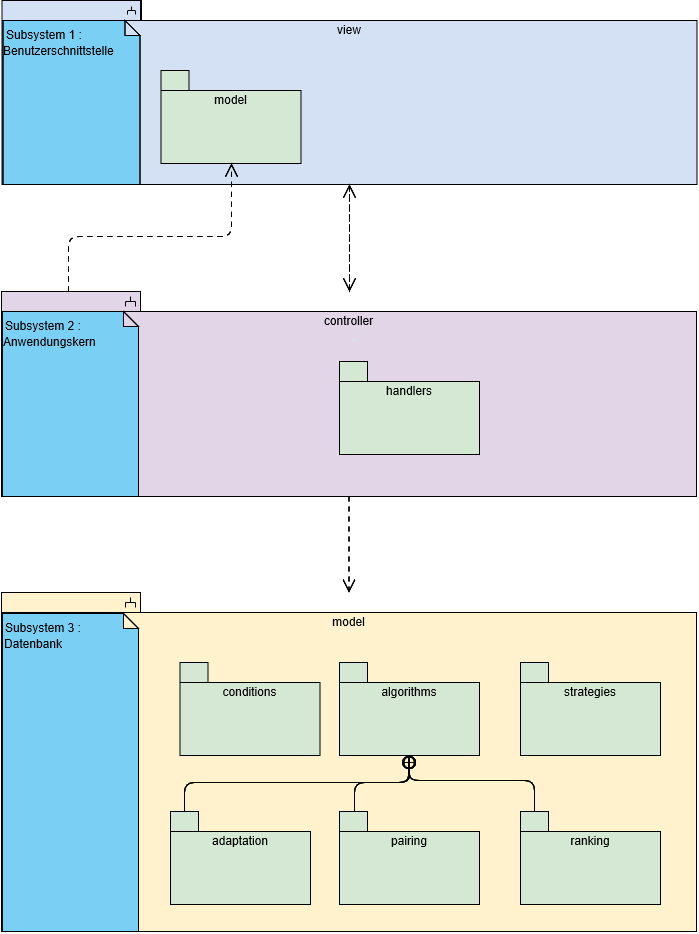
\includegraphics[width=1.1\textwidth]{UMLzuGrobentwurf}
\end{figure}

\subsection{Controller}

\noindent
\makebox[\textwidth]{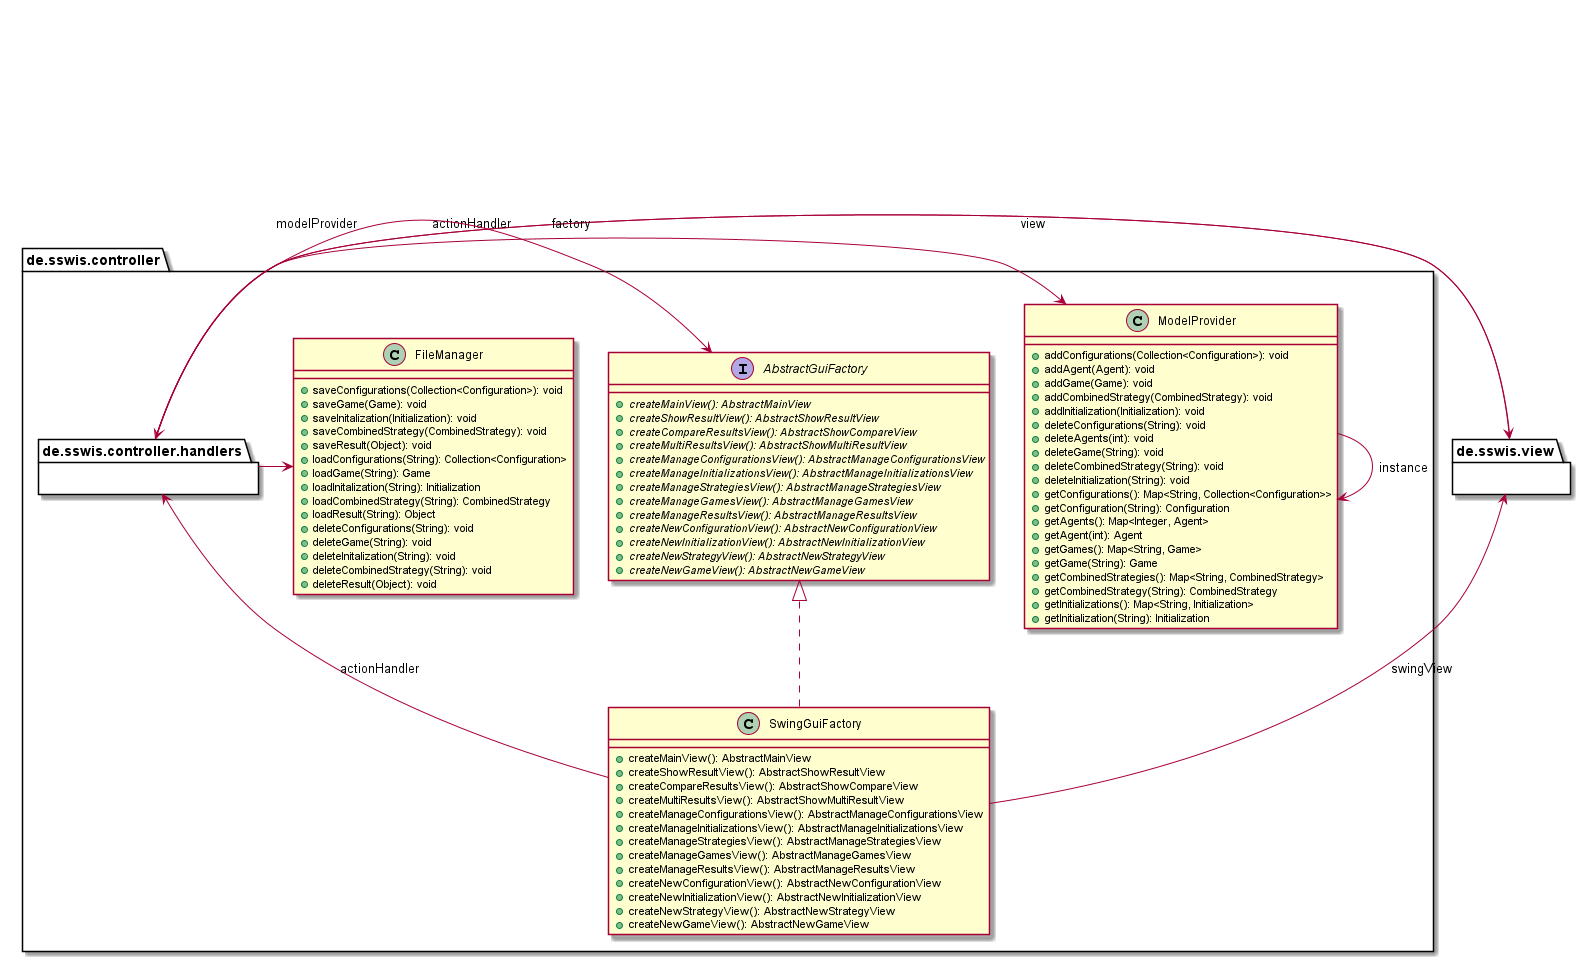
\includegraphics[scale=0.36]{Controller_package}}

Zur Erfüllung der oben angedeuteten Aufgaben steht dem Controller eine Reihe an weiteren Klassen neben den ActionListener-Klassen, die sich im Paket Handlers befinden, zur Verfügung.

Zum einen müssen die GUI-Objekte, d.h. alle Fenster mit denen der Benutzer interagiert, erstellt werden. Dies wird durch das Fabrik-Entwurfsmuster realisiert. Das AbstractGuiFactory-Interface gibt alle nötigen Ansichten vor und bietet weiterhin die oben beschriebene Möglichkeit, das Programm zu einem späteren Zeitpunkt komfortabel um neue Benutzeroberflächen zu erweitern.
Die SwingGuiFactory-Klasse erstellt die Objekte der von diesem Entwicklerteam angebotenen, Swing-basierten Benutzeroberfläche.

Bei dem ModelProvider handelt es sich um ein Einzelstück, das als zentrale Anlaufstelle für alle Model-Objekte dient. Das Einzelstück-Entwurfsmuster wurde verwendet, um Inkonsistenzen vorzubeugen.

Im FileManager werden Methoden zum Speichern, Laden und Löschen von Objekten bereitgestellt, die gesicherte Benutzereingaben und Ergebnisse darstellen. Das Bearbeiten dieser Objekte geschieht durch ein Laden und anschließendes Speichern des gegebenen Objekts.
Die Objekte werden in einem programminternen Verzeichnis gespeichert.

Die vom Programm angebotenen "Dienstleistungen", darunter fallen die diversen Algorithmentypen\footnote{Adaptionsalgorithmen, Paarungsalgorithmen und Bewertungsalgorithmen} sowie die verfügbaren Bedingungen und Basis-Strategien, können durch den ModelServiceLoader zur Verfügung gestellt werden.
Dies ist nötig, da sie auf Entwicklerebene um weitere Ausprägungen ergänzt werden können und diese ebenfalls an allen relevanten Stellen, z.B. im Auswahlfenster für den Benutzer, sichtbar sein sollen.

Der ModelParser überträgt das ViewModel in das Model. Konkret werden die im ViewModel auf Korrektheit überprüften Benutzereingaben in Objekte umgewandelt, mit denen eine Simulation durchgeführt werden kann. Andersherum werden die Daten abgelaufener Simulationen in ein Format konvertiert, das die View darstellen kann.

Schließlich können durch das Interface Simulationen überwacht werden, wobei der ViewNotifier die Benutzeroberfläche benachrichtigt, sobald eine Simulation abgeschlossen ist. Es findet eine Parallelisierung statt, wodurch die Benutzeroberfläche auch während einer Simulation aktiv bleibt.

\subsection{Model}

\noindent
\makebox[\textwidth]{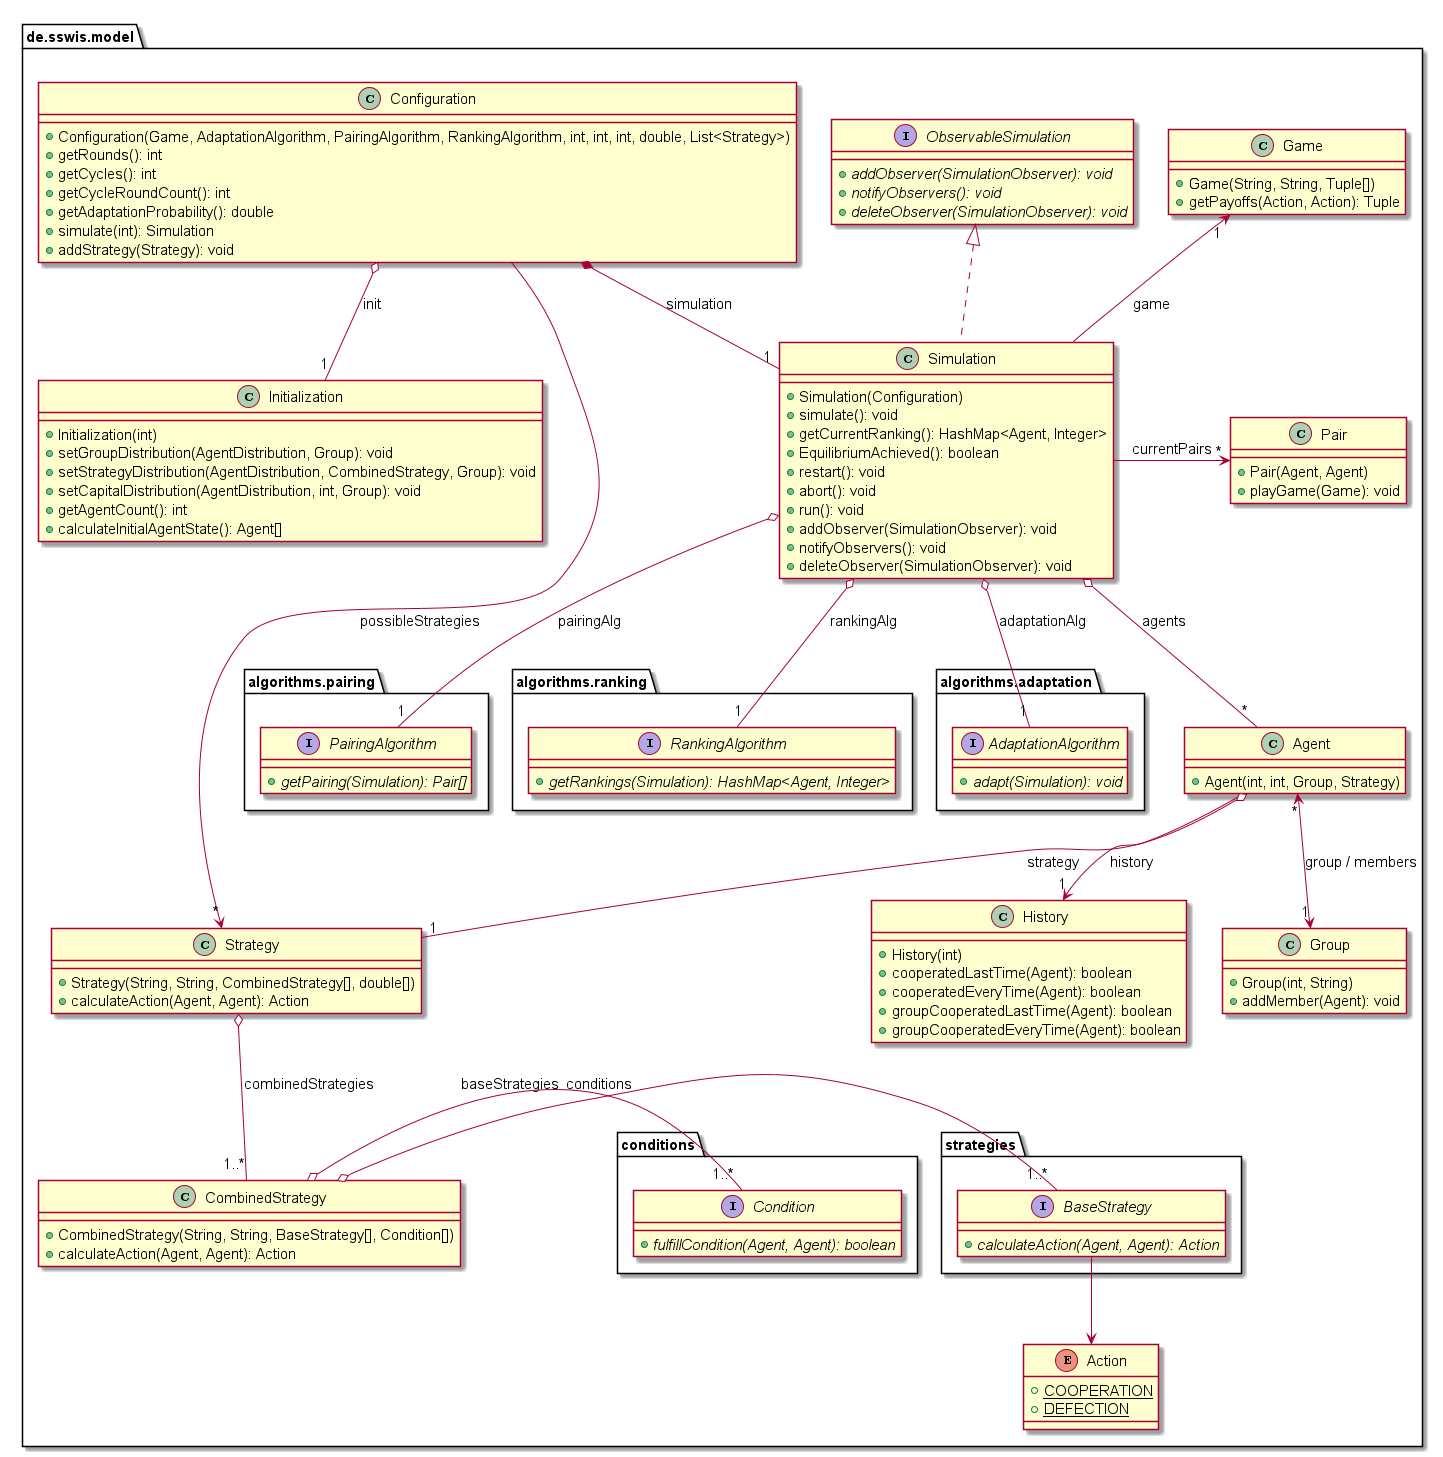
\includegraphics[scale=0.4]{model_classDiagramm}}


Im Model liegen alle Konfigurationen welche eine Simulation beschreiben. Jede Konfiguration besitzt eine Initialisierung, in der die initialen Zustände der Agenten beschrieben werden. \\

Eine Simulation implementiert eine Schnittstelle OberservableSimulation, um ein Observer zur Simulation hinzuzufügen. Hier wird das Entwurfsmuster Beobachter verwendet. Wenn eine Simulation terminiert, d.h. einen Gleichgewichtszustand oder die maximale Zyklenanzahl erreicht, sendet sie eine Nachricht an alle Observer.

In der Simulation werden zwei Agenten durch einen PairingAlgorithm gepaart, diese Paare spielen das ausgewählte Stufenspiel gegeneinander.

Es gibt drei Algorithmen Pakete im Model, welche die Simulation verwendet. Diese sind: 
\begin{itemize}
\item $algorithms.pairing$
\item $algorithms.ranking$
\item $algorithms.adaptation$
\end{itemize}
$algorithms.pairing$ bietet die verschiedenen Algorithmen für die Paarung vom Agenten. In $algorithms.ranking$ liegen die Algorithmen für die Bewertung der Agenten am Ende eines Zyklus. $algorithms.adaptation$ enthält die Algorithmen, welche die Strategien der Agenten am Ende eines Zyklus basierend auf dem Ranking anpassen. Bei den drei Paketen verwendet wir das Entwurfsmuster Strategie, um die Algorithmen während der Laufzeit dynamisch zu binden.

In den Paketen $strategies$ und $condition$ stehen die Basisstrategien und Bedingungen zur Verfügung. Mit diesen lassen sich kombinierte Strategien definieren, hier wird ebenfalls ein Strategie Entwurfsmuster verwendet. Die Klasse Strategy wiederum beschreibt eine gemischte Strategie, welche sich aus mehreren kombinierten Strategien zusammensetzt.

Ein History Objekt merkt sich die in einem Zyklus erreichten Punkte eines Agenten, sowie welche Agenten welche Aktionen gegen ihn gespielt haben. History Objekte werden dazu verwendet, um die Aktion in der aktuellen Runde eines Agenten zu ermitteln und Informationen über den Simulationsverlauf auf der Benutzeroberfläche anzuzeigen.


\subsection{View}

\noindent
\makebox[\textwidth]{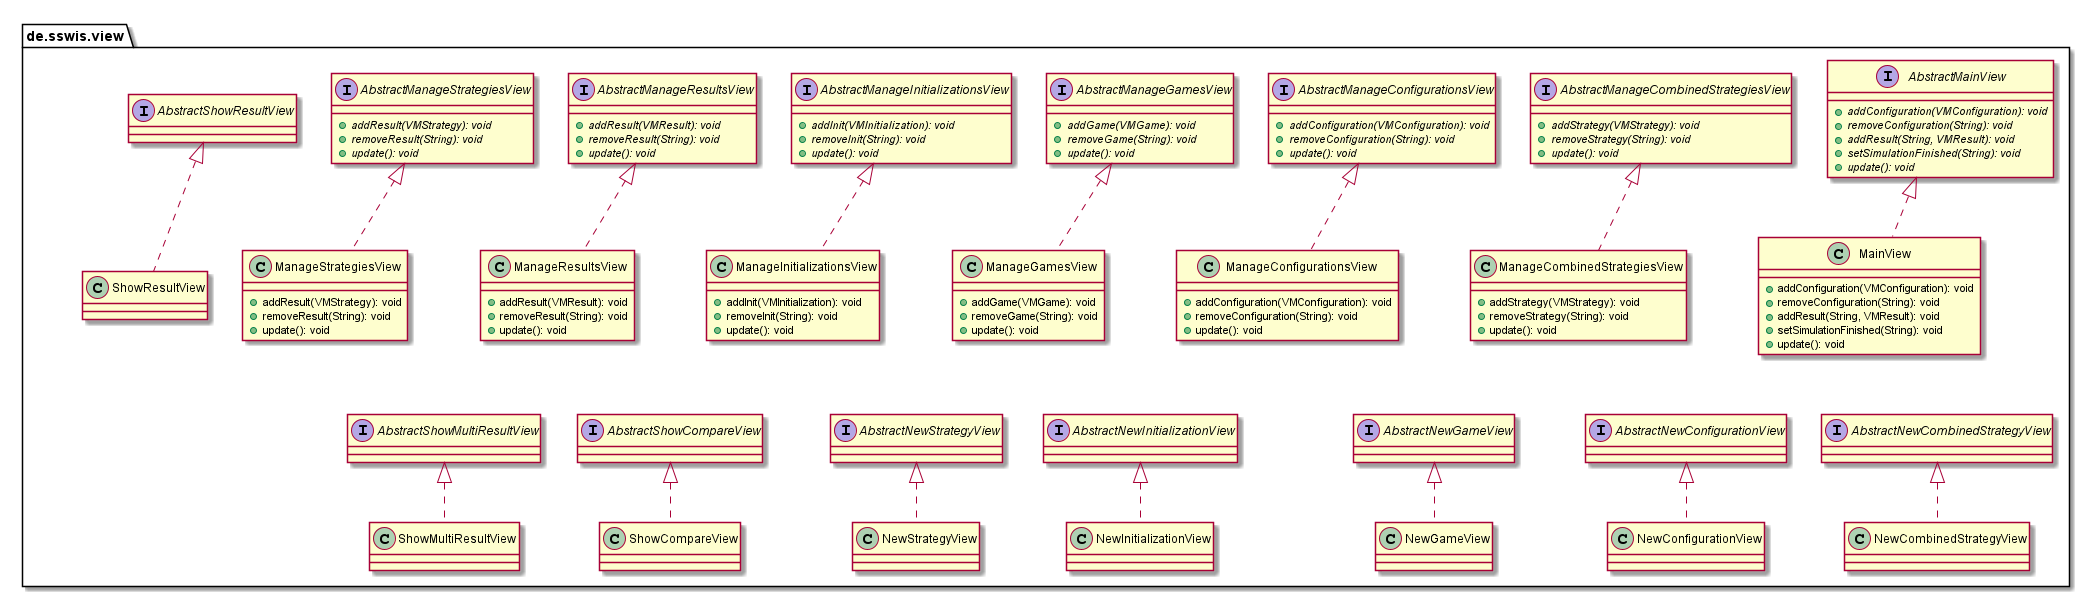
\includegraphics[scale=0.4]{view_classDiagramm}}

Für die Implementierung der Benutzeroberfläche wird die Java Swing Bibliothek und IntelliJ GUI Forms verwendet. In der View stehen alle Fenster, mit denen der Benutzer interagiert, als eigene Klasse zur Verfügung. Zur Übersicht sind nur drei dieser Klassen in dem Bild dargestellt, um das Zusammenspiel von View und View Model Objekten anschaulich zu machen.

Die Fenster enthalten Buttons und Menuitems, mit denen der Nutzer interagieren kann. Für diese werden die Handler aus dem Controller als ActionListener gesetzt.

Das Interface AbstractView enthält die grundlegendsten Methoden für ein GUI Fenster, um dieses anzeigen und schließen zu lassen. Jedes Fenster der Benutzeroberfläche implementiert ein eigenes Interface, das von AbtractView erbt und öffentliche Methoden, wie zum Beispiel zum Setzen der Actionlistener, enthält.

MainView ist das Hauptfenster des Programms. Es zeigt alle Konfigurationen an und über Buttons kann eine ausgewählte Konfiguration gestartet und die Ergebnisse angezeigt und gespeichert werden. Dafür besitzt das Fenster eine Liste aller gespeicherten VMConfiguration Objekte.
Über das Menü kann der Nutzer sich alle Fenster zum Verwalten und Erstellen von Konfigurationen, Initialisierungen, Stufenspielen und gemischten und kombinierten Strategien öffnen lassen.

ManageGamesView ist ein Fenster zum Verwalten von Stufenspielen. Über Buttons können Stufenspiele bearbeitet, gelöscht und erstellt werden. Damit Informationen zu allen Stufenspielen angezeigt werden können, besitzt das Fenster eine Liste aller gespeicherten VMGame Objekte. 

NewGameView ist ein Fenster zum Erstellen oder Bearbeiten eines Stufenspiels. Es besitzt ein VMGame Objekt, in das die Nutzereingaben übertragen werden. Das VMGame Objekt prüft dabei die Eingaben auf Korrektheit. 


\newpage
\section{Class Hierarchy}{

\subsection{Classes}
{\raggedright
\hspace{0.0cm} $\bullet$ java.lang.Object {\tiny \refdefined{java.lang.Object}} \\
\hspace{1.0cm} $\bullet$ de.sswis.controller.FileManager {\tiny \refdefined{de.sswis.controller.FileManager}} \\
\hspace{1.0cm} $\bullet$ de.sswis.controller.ModelParser {\tiny \refdefined{de.sswis.controller.ModelParser}} \\
\hspace{1.0cm} $\bullet$ de.sswis.controller.ModelProvider {\tiny \refdefined{de.sswis.controller.ModelProvider}} \\
\hspace{1.0cm} $\bullet$ de.sswis.controller.ModelServiceLoader {\tiny \refdefined{de.sswis.controller.ModelServiceLoader}} \\
\hspace{1.0cm} $\bullet$ de.sswis.controller.SwingGuiFactory {\tiny \refdefined{de.sswis.controller.SwingGuiFactory}} \\
\hspace{1.0cm} $\bullet$ de.sswis.controller.ViewNotifier {\tiny \refdefined{de.sswis.controller.ViewNotifier}} \\
\hspace{1.0cm} $\bullet$ de.sswis.controller.handlers.CancleHandler {\tiny \refdefined{de.sswis.controller.handlers.CancleHandler}} \\
\hspace{1.0cm} $\bullet$ de.sswis.controller.handlers.CompareResultsHandler {\tiny \refdefined{de.sswis.controller.handlers.CompareResultsHandler}} \\
\hspace{1.0cm} $\bullet$ de.sswis.controller.handlers.DeleteCombinedStrategyHandler {\tiny \refdefined{de.sswis.controller.handlers.DeleteCombinedStrategyHandler}} \\
\hspace{1.0cm} $\bullet$ de.sswis.controller.handlers.DeleteConfigurationHandler {\tiny \refdefined{de.sswis.controller.handlers.DeleteConfigurationHandler}} \\
\hspace{1.0cm} $\bullet$ de.sswis.controller.handlers.DeleteGameHandler {\tiny \refdefined{de.sswis.controller.handlers.DeleteGameHandler}} \\
\hspace{1.0cm} $\bullet$ de.sswis.controller.handlers.DeleteInitializationHandler {\tiny \refdefined{de.sswis.controller.handlers.DeleteInitializationHandler}} \\
\hspace{1.0cm} $\bullet$ de.sswis.controller.handlers.DeleteResultHandler {\tiny \refdefined{de.sswis.controller.handlers.DeleteResultHandler}} \\
\hspace{1.0cm} $\bullet$ de.sswis.controller.handlers.DeleteStrategyHandler {\tiny \refdefined{de.sswis.controller.handlers.DeleteStrategyHandler}} \\
\hspace{1.0cm} $\bullet$ de.sswis.controller.handlers.EditCombinedStrategyHandler {\tiny \refdefined{de.sswis.controller.handlers.EditCombinedStrategyHandler}} \\
\hspace{1.0cm} $\bullet$ de.sswis.controller.handlers.EditConfigurationHandler {\tiny \refdefined{de.sswis.controller.handlers.EditConfigurationHandler}} \\
\hspace{1.0cm} $\bullet$ de.sswis.controller.handlers.EditGameHandler {\tiny \refdefined{de.sswis.controller.handlers.EditGameHandler}} \\
\hspace{1.0cm} $\bullet$ de.sswis.controller.handlers.EditInitializationHandler {\tiny \refdefined{de.sswis.controller.handlers.EditInitializationHandler}} \\
\hspace{1.0cm} $\bullet$ de.sswis.controller.handlers.EditStrategyHandler {\tiny \refdefined{de.sswis.controller.handlers.EditStrategyHandler}} \\
\hspace{1.0cm} $\bullet$ de.sswis.controller.handlers.ManageCombinedStrategiesHandler {\tiny \refdefined{de.sswis.controller.handlers.ManageCombinedStrategiesHandler}} \\
\hspace{1.0cm} $\bullet$ de.sswis.controller.handlers.ManageConfigurationsHandler {\tiny \refdefined{de.sswis.controller.handlers.ManageConfigurationsHandler}} \\
\hspace{1.0cm} $\bullet$ de.sswis.controller.handlers.ManageGamesHandler {\tiny \refdefined{de.sswis.controller.handlers.ManageGamesHandler}} \\
\hspace{1.0cm} $\bullet$ de.sswis.controller.handlers.ManageInitializationHandler {\tiny \refdefined{de.sswis.controller.handlers.ManageInitializationHandler}} \\
\hspace{1.0cm} $\bullet$ de.sswis.controller.handlers.ManageResultsHandler {\tiny \refdefined{de.sswis.controller.handlers.ManageResultsHandler}} \\
\hspace{1.0cm} $\bullet$ de.sswis.controller.handlers.ManageStrategiesHandler {\tiny \refdefined{de.sswis.controller.handlers.ManageStrategiesHandler}} \\
\hspace{1.0cm} $\bullet$ de.sswis.controller.handlers.NewCombinedStrategyHandler {\tiny \refdefined{de.sswis.controller.handlers.NewCombinedStrategyHandler}} \\
\hspace{1.0cm} $\bullet$ de.sswis.controller.handlers.NewCombinedStrategyViewHandler {\tiny \refdefined{de.sswis.controller.handlers.NewCombinedStrategyViewHandler}} \\
\hspace{1.0cm} $\bullet$ de.sswis.controller.handlers.NewConfigurationHandler {\tiny \refdefined{de.sswis.controller.handlers.NewConfigurationHandler}} \\
\hspace{1.0cm} $\bullet$ de.sswis.controller.handlers.NewConfigurationViewHandler {\tiny \refdefined{de.sswis.controller.handlers.NewConfigurationViewHandler}} \\
\hspace{1.0cm} $\bullet$ de.sswis.controller.handlers.NewGameHandler {\tiny \refdefined{de.sswis.controller.handlers.NewGameHandler}} \\
\hspace{1.0cm} $\bullet$ de.sswis.controller.handlers.NewGameViewHandler {\tiny \refdefined{de.sswis.controller.handlers.NewGameViewHandler}} \\
\hspace{1.0cm} $\bullet$ de.sswis.controller.handlers.NewInitializationHandler {\tiny \refdefined{de.sswis.controller.handlers.NewInitializationHandler}} \\
\hspace{1.0cm} $\bullet$ de.sswis.controller.handlers.NewInitializationViewHandler {\tiny \refdefined{de.sswis.controller.handlers.NewInitializationViewHandler}} \\
\hspace{1.0cm} $\bullet$ de.sswis.controller.handlers.NewStrategyHandler {\tiny \refdefined{de.sswis.controller.handlers.NewStrategyHandler}} \\
\hspace{1.0cm} $\bullet$ de.sswis.controller.handlers.NewStrategyViewHandler {\tiny \refdefined{de.sswis.controller.handlers.NewStrategyViewHandler}} \\
\hspace{1.0cm} $\bullet$ de.sswis.controller.handlers.SaveAndQuitHandler {\tiny \refdefined{de.sswis.controller.handlers.SaveAndQuitHandler}} \\
\hspace{1.0cm} $\bullet$ de.sswis.controller.handlers.SaveCombinedStrategiesHandler {\tiny \refdefined{de.sswis.controller.handlers.SaveCombinedStrategiesHandler}} \\
\hspace{1.0cm} $\bullet$ de.sswis.controller.handlers.SaveConfigurationsHandler {\tiny \refdefined{de.sswis.controller.handlers.SaveConfigurationsHandler}} \\
\hspace{1.0cm} $\bullet$ de.sswis.controller.handlers.SaveGamesHandler {\tiny \refdefined{de.sswis.controller.handlers.SaveGamesHandler}} \\
\hspace{1.0cm} $\bullet$ de.sswis.controller.handlers.SaveInitializationsHandler {\tiny \refdefined{de.sswis.controller.handlers.SaveInitializationsHandler}} \\
\hspace{1.0cm} $\bullet$ de.sswis.controller.handlers.SaveResultsHandler {\tiny \refdefined{de.sswis.controller.handlers.SaveResultsHandler}} \\
\hspace{1.0cm} $\bullet$ de.sswis.controller.handlers.SaveStrategiesHandler {\tiny \refdefined{de.sswis.controller.handlers.SaveStrategiesHandler}} \\
\hspace{1.0cm} $\bullet$ de.sswis.controller.handlers.ShowResultsHandler {\tiny \refdefined{de.sswis.controller.handlers.ShowResultsHandler}} \\
\hspace{1.0cm} $\bullet$ de.sswis.controller.handlers.StartSimulationHandler {\tiny \refdefined{de.sswis.controller.handlers.StartSimulationHandler}} \\
\hspace{1.0cm} $\bullet$ de.sswis.controller.handlers.StopSimulationHandler {\tiny \refdefined{de.sswis.controller.handlers.StopSimulationHandler}} \\
\hspace{1.0cm} $\bullet$ de.sswis.model.Agent {\tiny \refdefined{de.sswis.model.Agent}} \\
\hspace{1.0cm} $\bullet$ de.sswis.model.CombinedStrategy {\tiny \refdefined{de.sswis.model.CombinedStrategy}} \\
\hspace{1.0cm} $\bullet$ de.sswis.model.Configuration {\tiny \refdefined{de.sswis.model.Configuration}} \\
\hspace{1.0cm} $\bullet$ de.sswis.model.Game {\tiny \refdefined{de.sswis.model.Game}} \\
\hspace{1.0cm} $\bullet$ de.sswis.model.Game.Tuple {\tiny \refdefined{de.sswis.model.Game.Tuple}} \\
\hspace{1.0cm} $\bullet$ de.sswis.model.Group {\tiny \refdefined{de.sswis.model.Group}} \\
\hspace{1.0cm} $\bullet$ de.sswis.model.History {\tiny \refdefined{de.sswis.model.History}} \\
\hspace{1.0cm} $\bullet$ de.sswis.model.Initialization {\tiny \refdefined{de.sswis.model.Initialization}} \\
\hspace{1.0cm} $\bullet$ de.sswis.model.Pair {\tiny \refdefined{de.sswis.model.Pair}} \\
\hspace{1.0cm} $\bullet$ de.sswis.model.Simulation {\tiny \refdefined{de.sswis.model.Simulation}} \\
\hspace{1.0cm} $\bullet$ de.sswis.model.Strategy {\tiny \refdefined{de.sswis.model.Strategy}} \\
\hspace{1.0cm} $\bullet$ de.sswis.model.algorithms.adaptation.MixedLinearInterpolation {\tiny \refdefined{de.sswis.model.algorithms.adaptation.MixedLinearInterpolation}} \\
\hspace{1.0cm} $\bullet$ de.sswis.model.algorithms.adaptation.MixedSum {\tiny \refdefined{de.sswis.model.algorithms.adaptation.MixedSum}} \\
\hspace{1.0cm} $\bullet$ de.sswis.model.algorithms.adaptation.RandomAdaptation {\tiny \refdefined{de.sswis.model.algorithms.adaptation.RandomAdaptation}} \\
\hspace{1.0cm} $\bullet$ de.sswis.model.algorithms.adaptation.RankPercentage {\tiny \refdefined{de.sswis.model.algorithms.adaptation.RankPercentage}} \\
\hspace{1.0cm} $\bullet$ de.sswis.model.algorithms.adaptation.ReplicatorDynamicRank {\tiny \refdefined{de.sswis.model.algorithms.adaptation.ReplicatorDynamicRank}} \\
\hspace{1.0cm} $\bullet$ de.sswis.model.algorithms.adaptation.ReplicatorDynamicScore {\tiny \refdefined{de.sswis.model.algorithms.adaptation.ReplicatorDynamicScore}} \\
\hspace{1.0cm} $\bullet$ de.sswis.model.algorithms.pairing.BruteForcePairing {\tiny \refdefined{de.sswis.model.algorithms.pairing.BruteForcePairing}} \\
\hspace{1.0cm} $\bullet$ de.sswis.model.algorithms.pairing.BruteForcePairingHeuristic {\tiny \refdefined{de.sswis.model.algorithms.pairing.BruteForcePairingHeuristic}} \\
\hspace{1.0cm} $\bullet$ de.sswis.model.algorithms.pairing.MaximumWeightMatching {\tiny \refdefined{de.sswis.model.algorithms.pairing.MaximumWeightMatching}} \\
\hspace{1.0cm} $\bullet$ de.sswis.model.algorithms.pairing.RandomPairing {\tiny \refdefined{de.sswis.model.algorithms.pairing.RandomPairing}} \\
\hspace{1.0cm} $\bullet$ de.sswis.model.algorithms.ranking.AverageRank {\tiny \refdefined{de.sswis.model.algorithms.ranking.AverageRank}} \\
\hspace{1.0cm} $\bullet$ de.sswis.model.algorithms.ranking.CurrentCycleScore {\tiny \refdefined{de.sswis.model.algorithms.ranking.CurrentCycleScore}} \\
\hspace{1.0cm} $\bullet$ de.sswis.model.algorithms.ranking.CustomCycleScore {\tiny \refdefined{de.sswis.model.algorithms.ranking.CustomCycleScore}} \\
\hspace{1.0cm} $\bullet$ de.sswis.model.algorithms.ranking.Score {\tiny \refdefined{de.sswis.model.algorithms.ranking.Score}} \\
\hspace{1.0cm} $\bullet$ de.sswis.model.conditions.Always {\tiny \refdefined{de.sswis.model.conditions.Always}} \\
\hspace{1.0cm} $\bullet$ de.sswis.model.conditions.Delta {\tiny \refdefined{de.sswis.model.conditions.Delta}} \\
\hspace{1.0cm} $\bullet$ de.sswis.model.conditions.OwnGroup {\tiny \refdefined{de.sswis.model.conditions.OwnGroup}} \\
\hspace{1.0cm} $\bullet$ de.sswis.model.conditions.Poorer {\tiny \refdefined{de.sswis.model.conditions.Poorer}} \\
\hspace{1.0cm} $\bullet$ de.sswis.model.conditions.Probability {\tiny \refdefined{de.sswis.model.conditions.Probability}} \\
\hspace{1.0cm} $\bullet$ de.sswis.model.conditions.Richer {\tiny \refdefined{de.sswis.model.conditions.Richer}} \\
\hspace{1.0cm} $\bullet$ de.sswis.model.conditions.SpecificGroup {\tiny \refdefined{de.sswis.model.conditions.SpecificGroup}} \\
\hspace{1.0cm} $\bullet$ de.sswis.model.strategies.AlwaysCooperate {\tiny \refdefined{de.sswis.model.strategies.AlwaysCooperate}} \\
\hspace{1.0cm} $\bullet$ de.sswis.model.strategies.GrimEverybody {\tiny \refdefined{de.sswis.model.strategies.GrimEverybody}} \\
\hspace{1.0cm} $\bullet$ de.sswis.model.strategies.GrimIndividual {\tiny \refdefined{de.sswis.model.strategies.GrimIndividual}} \\
\hspace{1.0cm} $\bullet$ de.sswis.model.strategies.GroupGrim {\tiny \refdefined{de.sswis.model.strategies.GroupGrim}} \\
\hspace{1.0cm} $\bullet$ de.sswis.model.strategies.GroupTitForTat {\tiny \refdefined{de.sswis.model.strategies.GroupTitForTat}} \\
\hspace{1.0cm} $\bullet$ de.sswis.model.strategies.NeverCooperate {\tiny \refdefined{de.sswis.model.strategies.NeverCooperate}} \\
\hspace{1.0cm} $\bullet$ de.sswis.model.strategies.Random {\tiny \refdefined{de.sswis.model.strategies.Random}} \\
\hspace{1.0cm} $\bullet$ de.sswis.model.strategies.TitForTatEverybody {\tiny \refdefined{de.sswis.model.strategies.TitForTatEverybody}} \\
\hspace{1.0cm} $\bullet$ de.sswis.model.strategies.TitForTatIndividual {\tiny \refdefined{de.sswis.model.strategies.TitForTatIndividual}} \\
\hspace{1.0cm} $\bullet$ de.sswis.util.AgentDistribution {\tiny \refdefined{de.sswis.util.AgentDistribution}} \\
\hspace{1.0cm} $\bullet$ de.sswis.util.InputValidator {\tiny \refdefined{de.sswis.util.InputValidator}} \\
\hspace{1.0cm} $\bullet$ de.sswis.view.MainView {\tiny \refdefined{de.sswis.view.MainView}} \\
\hspace{1.0cm} $\bullet$ de.sswis.view.ManageCombinedStrategiesView {\tiny \refdefined{de.sswis.view.ManageCombinedStrategiesView}} \\
\hspace{1.0cm} $\bullet$ de.sswis.view.ManageConfigurationsView {\tiny \refdefined{de.sswis.view.ManageConfigurationsView}} \\
\hspace{1.0cm} $\bullet$ de.sswis.view.ManageGamesView {\tiny \refdefined{de.sswis.view.ManageGamesView}} \\
\hspace{1.0cm} $\bullet$ de.sswis.view.ManageInitializationsView {\tiny \refdefined{de.sswis.view.ManageInitializationsView}} \\
\hspace{1.0cm} $\bullet$ de.sswis.view.ManageResultsView {\tiny \refdefined{de.sswis.view.ManageResultsView}} \\
\hspace{1.0cm} $\bullet$ de.sswis.view.ManageStrategiesView {\tiny \refdefined{de.sswis.view.ManageStrategiesView}} \\
\hspace{1.0cm} $\bullet$ de.sswis.view.NewCombinedStrategyView {\tiny \refdefined{de.sswis.view.NewCombinedStrategyView}} \\
\hspace{1.0cm} $\bullet$ de.sswis.view.NewConfigurationView {\tiny \refdefined{de.sswis.view.NewConfigurationView}} \\
\hspace{1.0cm} $\bullet$ de.sswis.view.NewGameView {\tiny \refdefined{de.sswis.view.NewGameView}} \\
\hspace{1.0cm} $\bullet$ de.sswis.view.NewInitializationView {\tiny \refdefined{de.sswis.view.NewInitializationView}} \\
\hspace{1.0cm} $\bullet$ de.sswis.view.NewStrategyView {\tiny \refdefined{de.sswis.view.NewStrategyView}} \\
\hspace{1.0cm} $\bullet$ de.sswis.view.ShowCompareView {\tiny \refdefined{de.sswis.view.ShowCompareView}} \\
\hspace{1.0cm} $\bullet$ de.sswis.view.ShowMultiResultView {\tiny \refdefined{de.sswis.view.ShowMultiResultView}} \\
\hspace{1.0cm} $\bullet$ de.sswis.view.ShowResultView {\tiny \refdefined{de.sswis.view.ShowResultView}} \\
\hspace{1.0cm} $\bullet$ de.sswis.view.model.VMCombinedStrategy {\tiny \refdefined{de.sswis.view.model.VMCombinedStrategy}} \\
\hspace{1.0cm} $\bullet$ de.sswis.view.model.VMConfiguration {\tiny \refdefined{de.sswis.view.model.VMConfiguration}} \\
\hspace{1.0cm} $\bullet$ de.sswis.view.model.VMGame {\tiny \refdefined{de.sswis.view.model.VMGame}} \\
\hspace{1.0cm} $\bullet$ de.sswis.view.model.VMGroup {\tiny \refdefined{de.sswis.view.model.VMGroup}} \\
\hspace{1.0cm} $\bullet$ de.sswis.view.model.VMInitialization {\tiny \refdefined{de.sswis.view.model.VMInitialization}} \\
\hspace{1.0cm} $\bullet$ de.sswis.view.model.VMResult {\tiny \refdefined{de.sswis.view.model.VMResult}} \\
\hspace{1.0cm} $\bullet$ de.sswis.view.model.VMStrategy {\tiny \refdefined{de.sswis.view.model.VMStrategy}} \\
\hspace{1.0cm} $\bullet$ java.lang.Enum {\tiny \refdefined{java.lang.Enum}} \\
\hspace{2.0cm} $\bullet$ de.sswis.model.Action {\tiny \refdefined{de.sswis.model.Action}} \\
}
\subsection{Interfaces}
\hspace{0.0cm} $\bullet$ de.sswis.controller.AbstractGuiFactory {\tiny \refdefined{de.sswis.controller.AbstractGuiFactory}} \\
\hspace{0.0cm} $\bullet$ de.sswis.controller.SimulationObserver {\tiny \refdefined{de.sswis.controller.SimulationObserver}} \\
\hspace{0.0cm} $\bullet$ de.sswis.model.ObservableSimulation {\tiny \refdefined{de.sswis.model.ObservableSimulation}} \\
\hspace{0.0cm} $\bullet$ de.sswis.model.algorithms.adaptation.AdaptationAlgorithm {\tiny \refdefined{de.sswis.model.algorithms.adaptation.AdaptationAlgorithm}} \\
\hspace{0.0cm} $\bullet$ de.sswis.model.algorithms.pairing.PairingAlgorithm {\tiny \refdefined{de.sswis.model.algorithms.pairing.PairingAlgorithm}} \\
\hspace{0.0cm} $\bullet$ de.sswis.model.algorithms.ranking.RankingAlgorithm {\tiny \refdefined{de.sswis.model.algorithms.ranking.RankingAlgorithm}} \\
\hspace{0.0cm} $\bullet$ de.sswis.model.conditions.Condition {\tiny \refdefined{de.sswis.model.conditions.Condition}} \\
\hspace{0.0cm} $\bullet$ de.sswis.model.strategies.BaseStrategy {\tiny \refdefined{de.sswis.model.strategies.BaseStrategy}} \\
\hspace{0.0cm} $\bullet$ de.sswis.view.AbstractView {\tiny \refdefined{de.sswis.view.AbstractView}} \\
\hspace{1.0cm} $\bullet$ de.sswis.view.AbstractMainView {\tiny \refdefined{de.sswis.view.AbstractMainView}} \\
\hspace{1.0cm} $\bullet$ de.sswis.view.AbstractManageCombinedStrategiesView {\tiny \refdefined{de.sswis.view.AbstractManageCombinedStrategiesView}} \\
\hspace{1.0cm} $\bullet$ de.sswis.view.AbstractManageConfigurationsView {\tiny \refdefined{de.sswis.view.AbstractManageConfigurationsView}} \\
\hspace{1.0cm} $\bullet$ de.sswis.view.AbstractManageGamesView {\tiny \refdefined{de.sswis.view.AbstractManageGamesView}} \\
\hspace{1.0cm} $\bullet$ de.sswis.view.AbstractManageInitializationsView {\tiny \refdefined{de.sswis.view.AbstractManageInitializationsView}} \\
\hspace{1.0cm} $\bullet$ de.sswis.view.AbstractManageResultsView {\tiny \refdefined{de.sswis.view.AbstractManageResultsView}} \\
\hspace{1.0cm} $\bullet$ de.sswis.view.AbstractManageStrategiesView {\tiny \refdefined{de.sswis.view.AbstractManageStrategiesView}} \\
\hspace{1.0cm} $\bullet$ de.sswis.view.AbstractNewCombinedStrategyView {\tiny \refdefined{de.sswis.view.AbstractNewCombinedStrategyView}} \\
\hspace{1.0cm} $\bullet$ de.sswis.view.AbstractNewConfigurationView {\tiny \refdefined{de.sswis.view.AbstractNewConfigurationView}} \\
\hspace{1.0cm} $\bullet$ de.sswis.view.AbstractNewGameView {\tiny \refdefined{de.sswis.view.AbstractNewGameView}} \\
\hspace{1.0cm} $\bullet$ de.sswis.view.AbstractNewInitializationView {\tiny \refdefined{de.sswis.view.AbstractNewInitializationView}} \\
\hspace{1.0cm} $\bullet$ de.sswis.view.AbstractNewStrategyView {\tiny \refdefined{de.sswis.view.AbstractNewStrategyView}} \\
\hspace{1.0cm} $\bullet$ de.sswis.view.AbstractShowCompareView {\tiny \refdefined{de.sswis.view.AbstractShowCompareView}} \\
\hspace{1.0cm} $\bullet$ de.sswis.view.AbstractShowMultiResultView {\tiny \refdefined{de.sswis.view.AbstractShowMultiResultView}} \\
\hspace{1.0cm} $\bullet$ de.sswis.view.AbstractShowResultView {\tiny \refdefined{de.sswis.view.AbstractShowResultView}} \\
}
\section{Package de.sswis.controller}{
\label{de.sswis.controller}\hypertarget{de.sswis.controller}{}
\hskip -.05in
\hbox to \hsize{\textit{ Package Contents\hfil Page}}
\vskip .13in
\hbox{{\bf  Interfaces}}
\entityintro{AbstractGuiFactory}{de.sswis.controller.AbstractGuiFactory}{Eine Fabrik zum Erzeugen von GUIs.}
\entityintro{SimulationObserver}{de.sswis.controller.SimulationObserver}{Observer zum Beobachten von \texttt{\small \hyperlink{de.sswis.model.Simulation}{Simulationen}}{\small 
\refdefined{de.sswis.model.Simulation}}.}
\vskip .13in
\hbox{{\bf  Classes}}
\entityintro{FileManager}{de.sswis.controller.FileManager}{Verwaltet \texttt{\small ViewModel} Objekte in Dateien.}
\entityintro{ModelParser}{de.sswis.controller.ModelParser}{Übersetzt Objekte zwischen dem \texttt{\small ViewModel} und dem \texttt{\small Model}.}
\entityintro{ModelProvider}{de.sswis.controller.ModelProvider}{Verwaltet die Model-Objekte.}
\entityintro{ModelServiceLoader}{de.sswis.controller.ModelServiceLoader}{Ein Dienstleister zur Bereitstellung von Listen mit allen Ausprägungen eines bestimmten Algorithmentyps sowie von Bedingungen und Basis-Strategien.}
\entityintro{SwingGuiFactory}{de.sswis.controller.SwingGuiFactory}{Eine Fabrik zum Erzeugen von GUIs mit \texttt{\small Swing}.}
\entityintro{ViewNotifier}{de.sswis.controller.ViewNotifier}{Benachrichtigt die View über beendete \texttt{\small Simulationen}.}
\vskip .1in
\vskip .1in
\subsection{\label{de.sswis.controller.AbstractGuiFactory}Interface AbstractGuiFactory}{
\hypertarget{de.sswis.controller.AbstractGuiFactory}{}\vskip .1in 
Eine Fabrik zum Erzeugen von GUIs. Der Nutzer dieser Schnittstelle kann sich alle Benutzeroberflächen erzeugen lassen, die in Sswis verwendet werden können. Die Methoden liefern alle eine Schnittstelle zurück, welches das zu erzeugende Fenster beschreibt. In den Methoden werden die Instanzen der jeweiligen Klassen mit den entsprechenden Schnittstellen erzeugt und die benötigten \texttt{\small ActionListener} gesetzt. Bestimmte Implementierungen von Benutzeroberflächen können weitere oder andere Parameter benötigen.\mbox{}\newline Das \texttt{\small AbstractGuiFactory} Interface enthält eine Methode, um das Hauptfenster zu erzeugen.\mbox{}\newline Das \texttt{\small AbstractGuiFactory} Interface enthält eine Methode, um das Ergebnisansichtsfenster zu erzeugen.\mbox{}\newline Das \texttt{\small AbstractGuiFactory} Interface enthält fünf Methoden, um die Fenster zum Verwalten von Konfigurationen, Initialisierungen, Strategien, Spielen und Ergebnissen zu erzeugen.\mbox{}\newline Das \texttt{\small AbstractGuiFactory} Interface enthält vier Methoden, um die Fenster zum Erstellen von neuen Konfigurationen, Initialisierungen, Strategien und Spielen zu erzeugen.\vskip .1in 
\subsubsection{Declaration}{
\begin{lstlisting}[frame=none]
public interface AbstractGuiFactory
\end{lstlisting}
\subsubsection{All known subinterfaces}{SwingGuiFactory\small{\refdefined{de.sswis.controller.SwingGuiFactory}}}
\subsubsection{All classes known to implement interface}{SwingGuiFactory\small{\refdefined{de.sswis.controller.SwingGuiFactory}}}
\subsubsection{Methods}{
\vskip -2em
\begin{itemize}
\item{ 
\index{createCompareResultsView()}
\hypertarget{de.sswis.controller.AbstractGuiFactory.createCompareResultsView()}{{\bf  createCompareResultsView}\\}
\begin{lstlisting}[frame=none]
de.sswis.view.AbstractShowCompareView createCompareResultsView()\end{lstlisting} %end signature
\begin{itemize}
\item{
{\bf  Description}

Erstellt eine Ergebnisansicht zum Vergleichen von Simulationen.
}
\item{{\bf  Returns} -- 
eine Ergebnisansicht zum Vergleichen von Simulationen 
}%end item
\end{itemize}
}%end item
\item{ 
\index{createMainView()}
\hypertarget{de.sswis.controller.AbstractGuiFactory.createMainView()}{{\bf  createMainView}\\}
\begin{lstlisting}[frame=none]
de.sswis.view.AbstractMainView createMainView()\end{lstlisting} %end signature
\begin{itemize}
\item{
{\bf  Description}

Erstellt ein Hauptfenster.
}
\item{{\bf  Returns} -- 
ein Hauptfenster 
}%end item
\end{itemize}
}%end item
\item{ 
\index{createManageCombinedStrategiesView()}
\hypertarget{de.sswis.controller.AbstractGuiFactory.createManageCombinedStrategiesView()}{{\bf  createManageCombinedStrategiesView}\\}
\begin{lstlisting}[frame=none]
de.sswis.view.AbstractManageCombinedStrategiesView createManageCombinedStrategiesView()\end{lstlisting} %end signature
\begin{itemize}
\item{
{\bf  Description}

Erstellt ein Strategieverwaltungsfenster für kombinierte Strategien.
}
\item{{\bf  Returns} -- 
ein Strategieverwaltungsfenster für kombinierte Strategien 
}%end item
\end{itemize}
}%end item
\item{ 
\index{createManageConfigurationsView()}
\hypertarget{de.sswis.controller.AbstractGuiFactory.createManageConfigurationsView()}{{\bf  createManageConfigurationsView}\\}
\begin{lstlisting}[frame=none]
de.sswis.view.AbstractManageConfigurationsView createManageConfigurationsView()\end{lstlisting} %end signature
\begin{itemize}
\item{
{\bf  Description}

Erstellt ein Konfigurationsverwaltungsfenster.
}
\item{{\bf  Returns} -- 
ein Konfigurationsverwaltungsfenster 
}%end item
\end{itemize}
}%end item
\item{ 
\index{createManageGamesView()}
\hypertarget{de.sswis.controller.AbstractGuiFactory.createManageGamesView()}{{\bf  createManageGamesView}\\}
\begin{lstlisting}[frame=none]
de.sswis.view.AbstractManageGamesView createManageGamesView()\end{lstlisting} %end signature
\begin{itemize}
\item{
{\bf  Description}

Erstellt ein Spieleverwaltungsfenster.
}
\item{{\bf  Returns} -- 
ein Spieleverwaltungsfenster 
}%end item
\end{itemize}
}%end item
\item{ 
\index{createManageInitializationsView()}
\hypertarget{de.sswis.controller.AbstractGuiFactory.createManageInitializationsView()}{{\bf  createManageInitializationsView}\\}
\begin{lstlisting}[frame=none]
de.sswis.view.AbstractManageInitializationsView createManageInitializationsView()\end{lstlisting} %end signature
\begin{itemize}
\item{
{\bf  Description}

Erstellt ein Initialisierungsverwaltungsfenster.
}
\item{{\bf  Returns} -- 
ein Initialisierungsverwaltungsfenster 
}%end item
\end{itemize}
}%end item
\item{ 
\index{createManageResultsView()}
\hypertarget{de.sswis.controller.AbstractGuiFactory.createManageResultsView()}{{\bf  createManageResultsView}\\}
\begin{lstlisting}[frame=none]
de.sswis.view.AbstractManageResultsView createManageResultsView()\end{lstlisting} %end signature
\begin{itemize}
\item{
{\bf  Description}

Erstellt ein Ergebnisverwaltungsfenster.
}
\item{{\bf  Returns} -- 
ein Ergebnisverwaltungsfenster 
}%end item
\end{itemize}
}%end item
\item{ 
\index{createManageStrategiesView()}
\hypertarget{de.sswis.controller.AbstractGuiFactory.createManageStrategiesView()}{{\bf  createManageStrategiesView}\\}
\begin{lstlisting}[frame=none]
de.sswis.view.AbstractManageStrategiesView createManageStrategiesView()\end{lstlisting} %end signature
\begin{itemize}
\item{
{\bf  Description}

Erstellt ein Strategieverwaltungsfenster für gemischte Strategien.
}
\item{{\bf  Returns} -- 
ein Strategieverwaltungsfenster gür gemischte Strategien 
}%end item
\end{itemize}
}%end item
\item{ 
\index{createMultiResultsView()}
\hypertarget{de.sswis.controller.AbstractGuiFactory.createMultiResultsView()}{{\bf  createMultiResultsView}\\}
\begin{lstlisting}[frame=none]
de.sswis.view.AbstractShowMultiResultView createMultiResultsView()\end{lstlisting} %end signature
\begin{itemize}
\item{
{\bf  Description}

Erstellt eine Ergebnisansicht mit allen Simulationen einer Multikonfiguration.
}
\item{{\bf  Returns} -- 
eine Ergebnisansicht mit allen Simulationen einer Multikonfiguration 
}%end item
\end{itemize}
}%end item
\item{ 
\index{createNewCombinedStrategyView()}
\hypertarget{de.sswis.controller.AbstractGuiFactory.createNewCombinedStrategyView()}{{\bf  createNewCombinedStrategyView}\\}
\begin{lstlisting}[frame=none]
de.sswis.view.AbstractNewCombinedStrategyView createNewCombinedStrategyView()\end{lstlisting} %end signature
\begin{itemize}
\item{
{\bf  Description}

Erstellt ein Fenster zum Erstellen von kombinierten Strategien.
}
\item{{\bf  Returns} -- 
ein Fenster zum Erstellen von kombinierten Strategien 
}%end item
\end{itemize}
}%end item
\item{ 
\index{createNewConfigurationView()}
\hypertarget{de.sswis.controller.AbstractGuiFactory.createNewConfigurationView()}{{\bf  createNewConfigurationView}\\}
\begin{lstlisting}[frame=none]
de.sswis.view.AbstractNewConfigurationView createNewConfigurationView()\end{lstlisting} %end signature
\begin{itemize}
\item{
{\bf  Description}

Erstellt ein Fenster zum Erstellen von Konfigurationen.
}
\item{{\bf  Returns} -- 
ein Fenster zum Erstellen von Konfigurationen 
}%end item
\end{itemize}
}%end item
\item{ 
\index{createNewGameView()}
\hypertarget{de.sswis.controller.AbstractGuiFactory.createNewGameView()}{{\bf  createNewGameView}\\}
\begin{lstlisting}[frame=none]
de.sswis.view.AbstractNewGameView createNewGameView()\end{lstlisting} %end signature
\begin{itemize}
\item{
{\bf  Description}

Erstellt ein Fenster zum Erstellen von Spielen.
}
\item{{\bf  Returns} -- 
ein Fenster zum Erstellen von Spielen 
}%end item
\end{itemize}
}%end item
\item{ 
\index{createNewInitializationView()}
\hypertarget{de.sswis.controller.AbstractGuiFactory.createNewInitializationView()}{{\bf  createNewInitializationView}\\}
\begin{lstlisting}[frame=none]
de.sswis.view.AbstractNewInitializationView createNewInitializationView()\end{lstlisting} %end signature
\begin{itemize}
\item{
{\bf  Description}

Erstellt ein Fenster zum Erstellen von Initialisierungen.
}
\item{{\bf  Returns} -- 
ein Fenster zum Erstellen von Initialisierungen 
}%end item
\end{itemize}
}%end item
\item{ 
\index{createNewStrategyView()}
\hypertarget{de.sswis.controller.AbstractGuiFactory.createNewStrategyView()}{{\bf  createNewStrategyView}\\}
\begin{lstlisting}[frame=none]
de.sswis.view.AbstractNewStrategyView createNewStrategyView()\end{lstlisting} %end signature
\begin{itemize}
\item{
{\bf  Description}

Erstellt ein Fenster zum Erstellen von gemischten Strategien.
}
\item{{\bf  Returns} -- 
ein Fenster zum Erstellen von gemischten Strategien 
}%end item
\end{itemize}
}%end item
\item{ 
\index{createShowResultView()}
\hypertarget{de.sswis.controller.AbstractGuiFactory.createShowResultView()}{{\bf  createShowResultView}\\}
\begin{lstlisting}[frame=none]
de.sswis.view.AbstractShowResultView createShowResultView()\end{lstlisting} %end signature
\begin{itemize}
\item{
{\bf  Description}

Erstellt ein Ergebnisansichtsfenster.
}
\item{{\bf  Returns} -- 
ein Ergebnisansichtsfenster 
}%end item
\end{itemize}
}%end item
\end{itemize}
}
}
\subsection{\label{de.sswis.controller.SimulationObserver}Interface SimulationObserver}{
\hypertarget{de.sswis.controller.SimulationObserver}{}\vskip .1in 
Observer zum Beobachten von \texttt{\small \hyperlink{de.sswis.model.Simulation}{Simulationen}}{\small 
\refdefined{de.sswis.model.Simulation}}. Sobald eine \texttt{\small Simulation} terminiert hat, benachrichtigt sie alle ihre \texttt{\small SimulationObserver}.\mbox{}\newline Hinweis: Wir verwenden hier nicht das \texttt{\small Observer} Interface von Java, da es als \texttt{\small Deprecated} markiert wurde.\vskip .1in 
\subsubsection{Declaration}{
\begin{lstlisting}[frame=none]
public interface SimulationObserver
\end{lstlisting}
\subsubsection{All known subinterfaces}{ViewNotifier\small{\refdefined{de.sswis.controller.ViewNotifier}}}
\subsubsection{All classes known to implement interface}{ViewNotifier\small{\refdefined{de.sswis.controller.ViewNotifier}}}
\subsubsection{Methods}{
\vskip -2em
\begin{itemize}
\item{ 
\index{update(Simulation)}
\hypertarget{de.sswis.controller.SimulationObserver.update(de.sswis.model.Simulation)}{{\bf  update}\\}
\begin{lstlisting}[frame=none]
void update(de.sswis.model.Simulation sim)\end{lstlisting} %end signature
\begin{itemize}
\item{
{\bf  Description}

Wird von der beobachteten \texttt{\small Simulation} aufgerufen, sobald sie einen Gleichgewichtszustand oder die maximale Zyklenanzahl erreicht hat.
}
\item{
{\bf  Parameters}
  \begin{itemize}
   \item{
\texttt{sim} -- die beendete \texttt{\small Simulation}}
  \end{itemize}
}%end item
\end{itemize}
}%end item
\end{itemize}
}
}
\subsection{\label{de.sswis.controller.FileManager}Class FileManager}{
\hypertarget{de.sswis.controller.FileManager}{}\vskip .1in 
Verwaltet \texttt{\small ViewModel} Objekte in Dateien. Dies beinhaltet das Speichern, Löschen, Laden eines Objekts und Laden aller Objekte eines Typs. Die \texttt{\small ViewModel} Objekte werden alle in einer eigenen Datei als Json-String gespeichert. Der Dateiname ist definiert als \texttt{\small \_.sswis}. Das Speicherverzeichnis befindet sich in der jar-Datei und kann nicht geändert werden.\vskip .1in 
\subsubsection{Declaration}{
\begin{lstlisting}[frame=none]
public class FileManager
 extends java.lang.Object\end{lstlisting}
\subsubsection{Constructors}{
\vskip -2em
\begin{itemize}
\item{ 
\index{FileManager()}
\hypertarget{de.sswis.controller.FileManager()}{{\bf  FileManager}\\}
\begin{lstlisting}[frame=none]
public FileManager()\end{lstlisting} %end signature
\begin{itemize}
\item{
{\bf  Description}

Standardkonstruktor
}
\end{itemize}
}%end item
\end{itemize}
}
\subsubsection{Methods}{
\vskip -2em
\begin{itemize}
\item{ 
\index{deleteCombinedStrategy(String)}
\hypertarget{de.sswis.controller.FileManager.deleteCombinedStrategy(java.lang.String)}{{\bf  deleteCombinedStrategy}\\}
\begin{lstlisting}[frame=none]
public void deleteCombinedStrategy(java.lang.String name)\end{lstlisting} %end signature
\begin{itemize}
\item{
{\bf  Description}

Löscht die gespeicherte \texttt{\small VMCombinedStrategy} mit dem angegebenen Namen. Der Name wird vom Benutzer beim Erstellen der kombinierten Strategie festegelegt.
}
\item{
{\bf  Parameters}
  \begin{itemize}
   \item{
\texttt{name} -- der Name der \texttt{\small VMCombinedStrategy}}
  \end{itemize}
}%end item
\end{itemize}
}%end item
\item{ 
\index{deleteConfiguration(String)}
\hypertarget{de.sswis.controller.FileManager.deleteConfiguration(java.lang.String)}{{\bf  deleteConfiguration}\\}
\begin{lstlisting}[frame=none]
public void deleteConfiguration(java.lang.String name)\end{lstlisting} %end signature
\begin{itemize}
\item{
{\bf  Description}

Löscht die gespeicherte \texttt{\small VMConfiguration} mit dem angegebenen Namen. Der Name wird vom Benutzer beim Erstellen der Konfiguration festegelegt.
}
\item{
{\bf  Parameters}
  \begin{itemize}
   \item{
\texttt{name} -- der Name der \texttt{\small VMConfiguration}}
  \end{itemize}
}%end item
\end{itemize}
}%end item
\item{ 
\index{deleteGame(String)}
\hypertarget{de.sswis.controller.FileManager.deleteGame(java.lang.String)}{{\bf  deleteGame}\\}
\begin{lstlisting}[frame=none]
public void deleteGame(java.lang.String name)\end{lstlisting} %end signature
\begin{itemize}
\item{
{\bf  Description}

Löscht das gespeicherte \texttt{\small VMGame} mit dem angegebenen Namen. Der Name wird vom Benutzer beim Erstellen des Stufenspiels festegelegt.
}
\item{
{\bf  Parameters}
  \begin{itemize}
   \item{
\texttt{name} -- der Name des \texttt{\small VMGame}}
  \end{itemize}
}%end item
\end{itemize}
}%end item
\item{ 
\index{deleteInitalization(String)}
\hypertarget{de.sswis.controller.FileManager.deleteInitalization(java.lang.String)}{{\bf  deleteInitalization}\\}
\begin{lstlisting}[frame=none]
public void deleteInitalization(java.lang.String name)\end{lstlisting} %end signature
\begin{itemize}
\item{
{\bf  Description}

Löscht die gespeicherte \texttt{\small VMInitialisation} mit dem angegebenen Namen. Der Name wird vom Benutzer beim Erstellen der Initialisierung festegelegt.
}
\item{
{\bf  Parameters}
  \begin{itemize}
   \item{
\texttt{name} -- der Name der \texttt{\small VMInitialisation}}
  \end{itemize}
}%end item
\end{itemize}
}%end item
\item{ 
\index{deleteResult(String)}
\hypertarget{de.sswis.controller.FileManager.deleteResult(java.lang.String)}{{\bf  deleteResult}\\}
\begin{lstlisting}[frame=none]
public void deleteResult(java.lang.String name)\end{lstlisting} %end signature
\begin{itemize}
\item{
{\bf  Description}

Löscht das gespeicherte \texttt{\small VMResult} mit dem angegebenen Namen. Der Name entspricht der zugehörigen \texttt{\small Configuration} aus deren Simulation das Ergebnis entstanden ist.
}
\item{
{\bf  Parameters}
  \begin{itemize}
   \item{
\texttt{name} -- der Name des \texttt{\small VMResult}}
  \end{itemize}
}%end item
\end{itemize}
}%end item
\item{ 
\index{loadAllCombinedStrategies()}
\hypertarget{de.sswis.controller.FileManager.loadAllCombinedStrategies()}{{\bf  loadAllCombinedStrategies}\\}
\begin{lstlisting}[frame=none]
public java.util.Collection loadAllCombinedStrategies()\end{lstlisting} %end signature
\begin{itemize}
\item{
{\bf  Description}

Lädt alle vorhandenen \texttt{\small VMCombinedStrategy} Objekte.
}
\item{{\bf  Returns} -- 
eine \texttt{\small Collection} von \texttt{\small VMCombinedStrategy} 
}%end item
\end{itemize}
}%end item
\item{ 
\index{loadAllConfigurations()}
\hypertarget{de.sswis.controller.FileManager.loadAllConfigurations()}{{\bf  loadAllConfigurations}\\}
\begin{lstlisting}[frame=none]
public java.util.Collection loadAllConfigurations()\end{lstlisting} %end signature
\begin{itemize}
\item{
{\bf  Description}

Lädt alle vorhandenen \texttt{\small VMConfiguration} Objekte.
}
\item{{\bf  Returns} -- 
eine \texttt{\small Collection} von \texttt{\small VMConfigurations} 
}%end item
\end{itemize}
}%end item
\item{ 
\index{loadAllGames()}
\hypertarget{de.sswis.controller.FileManager.loadAllGames()}{{\bf  loadAllGames}\\}
\begin{lstlisting}[frame=none]
public java.util.Collection loadAllGames()\end{lstlisting} %end signature
\begin{itemize}
\item{
{\bf  Description}

Lädt alle vorhandenen \texttt{\small VMGame} Objekte.
}
\item{{\bf  Returns} -- 
eine \texttt{\small Collection} von \texttt{\small VMGame} 
}%end item
\end{itemize}
}%end item
\item{ 
\index{loadAllInitializations()}
\hypertarget{de.sswis.controller.FileManager.loadAllInitializations()}{{\bf  loadAllInitializations}\\}
\begin{lstlisting}[frame=none]
public java.util.Collection loadAllInitializations()\end{lstlisting} %end signature
\begin{itemize}
\item{
{\bf  Description}

Lädt alle vorhandenen \texttt{\small VMInitialization} Objekte.
}
\item{{\bf  Returns} -- 
eine \texttt{\small Collection} von \texttt{\small VMInitialization} 
}%end item
\end{itemize}
}%end item
\item{ 
\index{loadAllResults()}
\hypertarget{de.sswis.controller.FileManager.loadAllResults()}{{\bf  loadAllResults}\\}
\begin{lstlisting}[frame=none]
public java.util.Collection loadAllResults()\end{lstlisting} %end signature
\begin{itemize}
\item{
{\bf  Description}

Lädt alle vorhandenen \texttt{\small VMResult} Objekte.
}
\item{{\bf  Returns} -- 
eine \texttt{\small Collection} von \texttt{\small VMResult} 
}%end item
\end{itemize}
}%end item
\item{ 
\index{loadCombinedStrategy(String)}
\hypertarget{de.sswis.controller.FileManager.loadCombinedStrategy(java.lang.String)}{{\bf  loadCombinedStrategy}\\}
\begin{lstlisting}[frame=none]
public de.sswis.view.model.VMCombinedStrategy loadCombinedStrategy(java.lang.String name)\end{lstlisting} %end signature
\begin{itemize}
\item{
{\bf  Description}

Lädt die \texttt{\small VMCombinedStrategy} mit dem angegebenen Namen. Der Name wird vom Benutzer beim Erstellen der kombinierten Strategie festegelegt.
}
\item{
{\bf  Parameters}
  \begin{itemize}
   \item{
\texttt{name} -- der Name der \texttt{\small VMCombinedStrategy}}
  \end{itemize}
}%end item
\item{{\bf  Returns} -- 
die \texttt{\small VMCombinedStrategy} mit dem angegebenen Namen 
}%end item
\end{itemize}
}%end item
\item{ 
\index{loadConfiguration(String)}
\hypertarget{de.sswis.controller.FileManager.loadConfiguration(java.lang.String)}{{\bf  loadConfiguration}\\}
\begin{lstlisting}[frame=none]
public de.sswis.view.model.VMConfiguration loadConfiguration(java.lang.String name)\end{lstlisting} %end signature
\begin{itemize}
\item{
{\bf  Description}

Lädt die \texttt{\small VMConfiguration} mit dem angegebenen Namen. Der Name wird vom Benutzer beim Erstellen der Konfiguration festegelegt.
}
\item{
{\bf  Parameters}
  \begin{itemize}
   \item{
\texttt{name} -- der Name der \texttt{\small VMConfiguration}}
  \end{itemize}
}%end item
\item{{\bf  Returns} -- 
die \texttt{\small VMConfiguration} mit dem angegebenen Namen 
}%end item
\end{itemize}
}%end item
\item{ 
\index{loadGame(String)}
\hypertarget{de.sswis.controller.FileManager.loadGame(java.lang.String)}{{\bf  loadGame}\\}
\begin{lstlisting}[frame=none]
public de.sswis.view.model.VMGame loadGame(java.lang.String name)\end{lstlisting} %end signature
\begin{itemize}
\item{
{\bf  Description}

Lädt das \texttt{\small VMGame} mit dem angegebenen Namen. Der Name wird vom Benutzer beim Erstellen des Stufenspiels festegelegt.
}
\item{
{\bf  Parameters}
  \begin{itemize}
   \item{
\texttt{name} -- der Name des \texttt{\small VMGame}}
  \end{itemize}
}%end item
\item{{\bf  Returns} -- 
das \texttt{\small VMGame} mit dem angegebenen Namen 
}%end item
\end{itemize}
}%end item
\item{ 
\index{loadInitalization(String)}
\hypertarget{de.sswis.controller.FileManager.loadInitalization(java.lang.String)}{{\bf  loadInitalization}\\}
\begin{lstlisting}[frame=none]
public de.sswis.view.model.VMInitialization loadInitalization(java.lang.String name)\end{lstlisting} %end signature
\begin{itemize}
\item{
{\bf  Description}

Lädt die \texttt{\small VMInitialization} mit dem angegebenen Namen. Der Name wird vom Benutzer beim Erstellen der Initialisierung festegelegt.
}
\item{
{\bf  Parameters}
  \begin{itemize}
   \item{
\texttt{name} -- der Name der \texttt{\small VMInitialization}}
  \end{itemize}
}%end item
\item{{\bf  Returns} -- 
die \texttt{\small VMInitialization} mit dem angegebenen Namen 
}%end item
\end{itemize}
}%end item
\item{ 
\index{loadResult(String)}
\hypertarget{de.sswis.controller.FileManager.loadResult(java.lang.String)}{{\bf  loadResult}\\}
\begin{lstlisting}[frame=none]
public de.sswis.view.model.VMResult loadResult(java.lang.String name)\end{lstlisting} %end signature
\begin{itemize}
\item{
{\bf  Description}

Lädt das \texttt{\small VMResult} mit dem angegebenen Namen. Der Name entspricht der zugehörigen \texttt{\small Configuration} aus deren Simulation das Ergebnis entstanden ist.
}
\item{
{\bf  Parameters}
  \begin{itemize}
   \item{
\texttt{name} -- der Name des \texttt{\small VMResult}}
  \end{itemize}
}%end item
\item{{\bf  Returns} -- 
das \texttt{\small VMResult} mit dem angegebenen Namen 
}%end item
\end{itemize}
}%end item
\item{ 
\index{saveCombinedStrategy(VMCombinedStrategy)}
\hypertarget{de.sswis.controller.FileManager.saveCombinedStrategy(de.sswis.view.model.VMCombinedStrategy)}{{\bf  saveCombinedStrategy}\\}
\begin{lstlisting}[frame=none]
public void saveCombinedStrategy(de.sswis.view.model.VMCombinedStrategy combinedStrategy)\end{lstlisting} %end signature
\begin{itemize}
\item{
{\bf  Description}

Speichert die gegebende \texttt{\small VMCombinedStrategy} in einer Datei.
}
\item{
{\bf  Parameters}
  \begin{itemize}
   \item{
\texttt{combinedStrategy} -- die zu speichernde \texttt{\small VMCombinedStrategy}}
  \end{itemize}
}%end item
\end{itemize}
}%end item
\item{ 
\index{saveConfiguration(VMConfiguration)}
\hypertarget{de.sswis.controller.FileManager.saveConfiguration(de.sswis.view.model.VMConfiguration)}{{\bf  saveConfiguration}\\}
\begin{lstlisting}[frame=none]
public void saveConfiguration(de.sswis.view.model.VMConfiguration configuration)\end{lstlisting} %end signature
\begin{itemize}
\item{
{\bf  Description}

Speichert die gegebende \texttt{\small VMConfiguration} in einer Datei.
}
\item{
{\bf  Parameters}
  \begin{itemize}
   \item{
\texttt{configuration} -- die zu speichernde \texttt{\small VMConfiguration}}
  \end{itemize}
}%end item
\end{itemize}
}%end item
\item{ 
\index{saveGame(VMGame)}
\hypertarget{de.sswis.controller.FileManager.saveGame(de.sswis.view.model.VMGame)}{{\bf  saveGame}\\}
\begin{lstlisting}[frame=none]
public void saveGame(de.sswis.view.model.VMGame game)\end{lstlisting} %end signature
\begin{itemize}
\item{
{\bf  Description}

Speichert das gegebende \texttt{\small VMGame} in einer Datei.
}
\item{
{\bf  Parameters}
  \begin{itemize}
   \item{
\texttt{game} -- das zu speichernde \texttt{\small VMGame}}
  \end{itemize}
}%end item
\end{itemize}
}%end item
\item{ 
\index{saveInitalization(VMInitialization)}
\hypertarget{de.sswis.controller.FileManager.saveInitalization(de.sswis.view.model.VMInitialization)}{{\bf  saveInitalization}\\}
\begin{lstlisting}[frame=none]
public void saveInitalization(de.sswis.view.model.VMInitialization initialization)\end{lstlisting} %end signature
\begin{itemize}
\item{
{\bf  Description}

Speichert die gegebende \texttt{\small VMInitialization} in einer Datei.
}
\item{
{\bf  Parameters}
  \begin{itemize}
   \item{
\texttt{initialization} -- die zu speichernde \texttt{\small VMInitialization}}
  \end{itemize}
}%end item
\end{itemize}
}%end item
\item{ 
\index{saveResult(VMResult)}
\hypertarget{de.sswis.controller.FileManager.saveResult(de.sswis.view.model.VMResult)}{{\bf  saveResult}\\}
\begin{lstlisting}[frame=none]
public void saveResult(de.sswis.view.model.VMResult result)\end{lstlisting} %end signature
\begin{itemize}
\item{
{\bf  Description}

Speichert das gegebende \texttt{\small VMResult} in einer Datei.
}
\item{
{\bf  Parameters}
  \begin{itemize}
   \item{
\texttt{result} -- das zu speichernde \texttt{\small VMResult}}
  \end{itemize}
}%end item
\end{itemize}
}%end item
\end{itemize}
}
}
\subsection{\label{de.sswis.controller.ModelParser}Class ModelParser}{
\hypertarget{de.sswis.controller.ModelParser}{}\vskip .1in 
Übersetzt Objekte zwischen dem \texttt{\small ViewModel} und dem \texttt{\small Model}. Dies dient primär dem Umsetzen von Benutzereingaben in eine lauffähige Simulation. Außerdem können Ergebnisse abgelaufener Simulationen für die Ergebnisansicht aufbereitet werden.\vskip .1in 
\subsubsection{Declaration}{
\begin{lstlisting}[frame=none]
public class ModelParser
 extends java.lang.Object\end{lstlisting}
\subsubsection{Constructors}{
\vskip -2em
\begin{itemize}
\item{ 
\index{ModelParser()}
\hypertarget{de.sswis.controller.ModelParser()}{{\bf  ModelParser}\\}
\begin{lstlisting}[frame=none]
public ModelParser()\end{lstlisting} %end signature
}%end item
\end{itemize}
}
\subsubsection{Methods}{
\vskip -2em
\begin{itemize}
\item{ 
\index{parseSimulationToVMResult(Simulation)}
\hypertarget{de.sswis.controller.ModelParser.parseSimulationToVMResult(de.sswis.model.Simulation)}{{\bf  parseSimulationToVMResult}\\}
\begin{lstlisting}[frame=none]
public de.sswis.view.model.VMResult parseSimulationToVMResult(de.sswis.model.Simulation simulation)\end{lstlisting} %end signature
\begin{itemize}
\item{
{\bf  Description}

Übersetzt das \texttt{\small Simulation}-Objekt einer abgeschlossenen Simulation in ein \texttt{\small VMResult}-Objekt. Dabei werden die Daten der Simulation in ein für die Ergebnisansicht konformes Format konvertiert.
}
\item{
{\bf  Parameters}
  \begin{itemize}
   \item{
\texttt{simulation} -- die abgeschlossene Simulation}
  \end{itemize}
}%end item
\item{{\bf  Returns} -- 
die für die Ergebnisansicht aufbereiteten Ergebnisse 
}%end item
\end{itemize}
}%end item
\item{ 
\index{parseVMCombinedStrategyToCombinedStrategy(VMCombinedStrategy)}
\hypertarget{de.sswis.controller.ModelParser.parseVMCombinedStrategyToCombinedStrategy(de.sswis.view.model.VMCombinedStrategy)}{{\bf  parseVMCombinedStrategyToCombinedStrategy}\\}
\begin{lstlisting}[frame=none]
public de.sswis.model.CombinedStrategy parseVMCombinedStrategyToCombinedStrategy(de.sswis.view.model.VMCombinedStrategy vmCombinedStrategy)\end{lstlisting} %end signature
\begin{itemize}
\item{
{\bf  Description}

Übersetzt ein \texttt{\small VMCombinedStrategy}-Objekt in ein \texttt{\small CombinedStrategy}-Objekt.
}
\item{
{\bf  Parameters}
  \begin{itemize}
   \item{
\texttt{vmCombinedStrategy} -- die zu übersetzende \texttt{\small VMCombinedStrategy}}
  \end{itemize}
}%end item
\item{{\bf  Returns} -- 
die übersetzte \texttt{\small CombinedStrategy} 
}%end item
\end{itemize}
}%end item
\item{ 
\index{parseVMConfigurationToConfigurations(VMConfiguration)}
\hypertarget{de.sswis.controller.ModelParser.parseVMConfigurationToConfigurations(de.sswis.view.model.VMConfiguration)}{{\bf  parseVMConfigurationToConfigurations}\\}
\begin{lstlisting}[frame=none]
public java.util.Collection parseVMConfigurationToConfigurations(de.sswis.view.model.VMConfiguration vmConfig)\end{lstlisting} %end signature
\begin{itemize}
\item{
{\bf  Description}

Übersetzt ein \texttt{\small VMConfiguration}-Objekt in eine Sammlung an \texttt{\small Configuration}-Objekten. Im Falle einer Mehrfachkonfiguration enthält die zurückgegebene Sammlung die \texttt{\small n} Einzelkonfigurationen.
}
\item{
{\bf  Parameters}
  \begin{itemize}
   \item{
\texttt{vmConfig} -- die zu übersetzende \texttt{\small VMConfiguration}}
  \end{itemize}
}%end item
\item{{\bf  Returns} -- 
die übersetzte \texttt{\small Collection} 
}%end item
\end{itemize}
}%end item
\item{ 
\index{parseVMGameToGame(VMGame)}
\hypertarget{de.sswis.controller.ModelParser.parseVMGameToGame(de.sswis.view.model.VMGame)}{{\bf  parseVMGameToGame}\\}
\begin{lstlisting}[frame=none]
public de.sswis.model.Game parseVMGameToGame(de.sswis.view.model.VMGame vmGame)\end{lstlisting} %end signature
\begin{itemize}
\item{
{\bf  Description}

Übersetzt ein \texttt{\small VMGame}-Objekt in ein \texttt{\small Game}-Objekt.
}
\item{
{\bf  Parameters}
  \begin{itemize}
   \item{
\texttt{vmGame} -- das zu übersetzende \texttt{\small VMGame}}
  \end{itemize}
}%end item
\item{{\bf  Returns} -- 
das übersetzte \texttt{\small Game} 
}%end item
\end{itemize}
}%end item
\item{ 
\index{parseVMGroupToGroup(VMGroup)}
\hypertarget{de.sswis.controller.ModelParser.parseVMGroupToGroup(de.sswis.view.model.VMGroup)}{{\bf  parseVMGroupToGroup}\\}
\begin{lstlisting}[frame=none]
public de.sswis.model.Group parseVMGroupToGroup(de.sswis.view.model.VMGroup vmGroup)\end{lstlisting} %end signature
\begin{itemize}
\item{
{\bf  Description}

Übersetzt ein \texttt{\small VMGroup}-Objekt in ein \texttt{\small Group}-Objekt.
}
\item{
{\bf  Parameters}
  \begin{itemize}
   \item{
\texttt{vmGroup} -- die zu übersetzende \texttt{\small VMGroup}}
  \end{itemize}
}%end item
\item{{\bf  Returns} -- 
die übersetzte \texttt{\small Group} 
}%end item
\end{itemize}
}%end item
\item{ 
\index{parseVMInitializationToInitialization(VMInitialization)}
\hypertarget{de.sswis.controller.ModelParser.parseVMInitializationToInitialization(de.sswis.view.model.VMInitialization)}{{\bf  parseVMInitializationToInitialization}\\}
\begin{lstlisting}[frame=none]
public java.util.Collection parseVMInitializationToInitialization(de.sswis.view.model.VMInitialization vmInitialization)\end{lstlisting} %end signature
\begin{itemize}
\item{
{\bf  Description}

Übersetzt ein \texttt{\small VMInitialization}-Objekt in eine Sammlung an \texttt{\small Initialization}-Objekten. Im Falle einer Mehrfachinitialisierung enthält die zurückgegebene Sammlung die \texttt{\small n} Einzelinitialisierungen.
}
\item{
{\bf  Parameters}
  \begin{itemize}
   \item{
\texttt{vmInitialization} -- die zu übersetzende \texttt{\small VMInitialization}}
  \end{itemize}
}%end item
\item{{\bf  Returns} -- 
die übersetzte \texttt{\small Collection} 
}%end item
\end{itemize}
}%end item
\item{ 
\index{parseVMStrategyToStrategy(VMStrategy)}
\hypertarget{de.sswis.controller.ModelParser.parseVMStrategyToStrategy(de.sswis.view.model.VMStrategy)}{{\bf  parseVMStrategyToStrategy}\\}
\begin{lstlisting}[frame=none]
public de.sswis.model.Strategy parseVMStrategyToStrategy(de.sswis.view.model.VMStrategy vmStrategy)\end{lstlisting} %end signature
\begin{itemize}
\item{
{\bf  Description}

Übersetzt ein \texttt{\small VMStrategy}-Objekt in ein \texttt{\small Strategy}-Objekt.
}
\item{
{\bf  Parameters}
  \begin{itemize}
   \item{
\texttt{vmStrategy} -- die zu übersetzende \texttt{\small VMStrategy}}
  \end{itemize}
}%end item
\item{{\bf  Returns} -- 
die übersetzte \texttt{\small Strategy} 
}%end item
\end{itemize}
}%end item
\end{itemize}
}
}
\subsection{\label{de.sswis.controller.ModelProvider}Class ModelProvider}{
\hypertarget{de.sswis.controller.ModelProvider}{}\vskip .1in 
Verwaltet die Model-Objekte. Alle erstellten \texttt{\small \hyperlink{de.sswis.model.Configuration}{Configurations}}{\small 
\refdefined{de.sswis.model.Configuration}}, \texttt{\small \hyperlink{de.sswis.model.Game}{Games}}{\small 
\refdefined{de.sswis.model.Game}}, \texttt{\small \hyperlink{de.sswis.model.CombinedStrategy}{CombinedStrategies}}{\small 
\refdefined{de.sswis.model.CombinedStrategy}} und \texttt{\small \hyperlink{de.sswis.model.Initialization}{Initializatoins}}{\small 
\refdefined{de.sswis.model.Initialization}} werden hier gespeichert, damit andere Controller-Objekte auf sie zugreifen können. Alle Objekte werden über ihren zugewiesenen Namen indentifiziert.\vskip .1in 
\subsubsection{Declaration}{
\begin{lstlisting}[frame=none]
public class ModelProvider
 extends java.lang.Object\end{lstlisting}
\subsubsection{Methods}{
\vskip -2em
\begin{itemize}
\item{ 
\index{addCombinedStrategy(CombinedStrategy)}
\hypertarget{de.sswis.controller.ModelProvider.addCombinedStrategy(de.sswis.model.CombinedStrategy)}{{\bf  addCombinedStrategy}\\}
\begin{lstlisting}[frame=none]
public void addCombinedStrategy(de.sswis.model.CombinedStrategy combStrategy)\end{lstlisting} %end signature
\begin{itemize}
\item{
{\bf  Description}

Fügt eine \texttt{\small CombinedStrategy} hinzu.
}
\item{
{\bf  Parameters}
  \begin{itemize}
   \item{
\texttt{combStrategy} -- die zu speichernde \texttt{\small CombinedStrategy}}
  \end{itemize}
}%end item
\end{itemize}
}%end item
\item{ 
\index{addConfigurations(Configuration)}
\hypertarget{de.sswis.controller.ModelProvider.addConfigurations(de.sswis.model.Configuration)}{{\bf  addConfigurations}\\}
\begin{lstlisting}[frame=none]
public void addConfigurations(de.sswis.model.Configuration configuration)\end{lstlisting} %end signature
\begin{itemize}
\item{
{\bf  Description}

Fügt eine \texttt{\small Collection} hinzu.
}
\item{
{\bf  Parameters}
  \begin{itemize}
   \item{
\texttt{configuration} -- die zu speichernde \texttt{\small Configurations}}
  \end{itemize}
}%end item
\end{itemize}
}%end item
\item{ 
\index{addGame(Game)}
\hypertarget{de.sswis.controller.ModelProvider.addGame(de.sswis.model.Game)}{{\bf  addGame}\\}
\begin{lstlisting}[frame=none]
public void addGame(de.sswis.model.Game game)\end{lstlisting} %end signature
\begin{itemize}
\item{
{\bf  Description}

Fügt ein \texttt{\small Game} hinzu.
}
\item{
{\bf  Parameters}
  \begin{itemize}
   \item{
\texttt{game} -- das zu speichernde \texttt{\small Game}}
  \end{itemize}
}%end item
\end{itemize}
}%end item
\item{ 
\index{addInitialization(Initialization)}
\hypertarget{de.sswis.controller.ModelProvider.addInitialization(de.sswis.model.Initialization)}{{\bf  addInitialization}\\}
\begin{lstlisting}[frame=none]
public void addInitialization(de.sswis.model.Initialization initialization)\end{lstlisting} %end signature
\begin{itemize}
\item{
{\bf  Description}

Fügt eine \texttt{\small Initialization} hinzu.
}
\item{
{\bf  Parameters}
  \begin{itemize}
   \item{
\texttt{initialization} -- die zu speichernde \texttt{\small Initialization}}
  \end{itemize}
}%end item
\end{itemize}
}%end item
\item{ 
\index{addStrategy(Strategy)}
\hypertarget{de.sswis.controller.ModelProvider.addStrategy(de.sswis.model.Strategy)}{{\bf  addStrategy}\\}
\begin{lstlisting}[frame=none]
public void addStrategy(de.sswis.model.Strategy strategy)\end{lstlisting} %end signature
\begin{itemize}
\item{
{\bf  Description}

Fügt eine \texttt{\small Strategy} hinzu
}
\item{
{\bf  Parameters}
  \begin{itemize}
   \item{
\texttt{strategy} -- die zu speichernde \texttt{\small Strategy}}
  \end{itemize}
}%end item
\end{itemize}
}%end item
\item{ 
\index{deleteCombinedStrategy(String)}
\hypertarget{de.sswis.controller.ModelProvider.deleteCombinedStrategy(java.lang.String)}{{\bf  deleteCombinedStrategy}\\}
\begin{lstlisting}[frame=none]
public void deleteCombinedStrategy(java.lang.String name)\end{lstlisting} %end signature
\begin{itemize}
\item{
{\bf  Description}

Löscht eine \texttt{\small CombinedStrategy}. Die \texttt{\small CombinedStrategy} wird über ihren Namen identifiziert. Löschen kann nicht rückgängig gemacht werden.
}
\item{
{\bf  Parameters}
  \begin{itemize}
   \item{
\texttt{name} -- Name der zu löschenden \texttt{\small CombinedStrategy}}
  \end{itemize}
}%end item
\end{itemize}
}%end item
\item{ 
\index{deleteConfiguration(String)}
\hypertarget{de.sswis.controller.ModelProvider.deleteConfiguration(java.lang.String)}{{\bf  deleteConfiguration}\\}
\begin{lstlisting}[frame=none]
public void deleteConfiguration(java.lang.String name)\end{lstlisting} %end signature
\begin{itemize}
\item{
{\bf  Description}

Löscht eine \texttt{\small Configuration}. Die \texttt{\small Configuration} wird über ihren Namen identifiziert. Löschen kann nicht rückgängig gemacht werden.
}
\item{
{\bf  Parameters}
  \begin{itemize}
   \item{
\texttt{name} -- Name der zu löschenden \texttt{\small Configuration}}
  \end{itemize}
}%end item
\end{itemize}
}%end item
\item{ 
\index{deleteGame(String)}
\hypertarget{de.sswis.controller.ModelProvider.deleteGame(java.lang.String)}{{\bf  deleteGame}\\}
\begin{lstlisting}[frame=none]
public void deleteGame(java.lang.String name)\end{lstlisting} %end signature
\begin{itemize}
\item{
{\bf  Description}

Löscht ein \texttt{\small Game}. Das \texttt{\small Game} wird über seinen Namen identifiziert. Löschen kann nicht rückgängig gemacht werden.
}
\item{
{\bf  Parameters}
  \begin{itemize}
   \item{
\texttt{name} -- Name des zu löschende \texttt{\small Game}}
  \end{itemize}
}%end item
\end{itemize}
}%end item
\item{ 
\index{deleteInitialization(String)}
\hypertarget{de.sswis.controller.ModelProvider.deleteInitialization(java.lang.String)}{{\bf  deleteInitialization}\\}
\begin{lstlisting}[frame=none]
public void deleteInitialization(java.lang.String name)\end{lstlisting} %end signature
\begin{itemize}
\item{
{\bf  Description}

Löscht eine \texttt{\small Initialization}. Die \texttt{\small Initialization} wird über ihren Namen identifiziert. Löschen kann nicht rückgängig geamacht werden.
}
\item{
{\bf  Parameters}
  \begin{itemize}
   \item{
\texttt{name} -- Name der zu löschenden \texttt{\small Initialization}}
  \end{itemize}
}%end item
\end{itemize}
}%end item
\item{ 
\index{deleteStrategy(String)}
\hypertarget{de.sswis.controller.ModelProvider.deleteStrategy(java.lang.String)}{{\bf  deleteStrategy}\\}
\begin{lstlisting}[frame=none]
public void deleteStrategy(java.lang.String name)\end{lstlisting} %end signature
\begin{itemize}
\item{
{\bf  Description}

Löscht eine \texttt{\small Strategy}. Die \texttt{\small Strategy} wird über ihren Namen identifiziert. Löschen kann nicht rückgängig gemacht werden.
}
\item{
{\bf  Parameters}
  \begin{itemize}
   \item{
\texttt{name} -- Name der zu löschenden \texttt{\small Strategy}}
  \end{itemize}
}%end item
\end{itemize}
}%end item
\item{ 
\index{getInstance()}
\hypertarget{de.sswis.controller.ModelProvider.getInstance()}{{\bf  getInstance}\\}
\begin{lstlisting}[frame=none]
public static ModelProvider getInstance()\end{lstlisting} %end signature
\begin{itemize}
\item{
{\bf  Description}

Gibt die Instanz dieser Klasse zurück. Es wird immer die gleiche Instanz zurück gegeben.
}
\item{{\bf  Returns} -- 
die Instanz dieser Klasse 
}%end item
\end{itemize}
}%end item
\end{itemize}
}
}
\subsection{\label{de.sswis.controller.ModelServiceLoader}Class ModelServiceLoader}{
\hypertarget{de.sswis.controller.ModelServiceLoader}{}\vskip .1in 
Ein Dienstleister zur Bereitstellung von Listen mit allen Ausprägungen eines bestimmten Algorithmentyps sowie von Bedingungen und Basis-Strategien. Die Algorithmentypen umfassen Adaptionsalgorithmen, Paarungsalgorithmen und Bewertungsalgorithmen.\vskip .1in 
\subsubsection{Declaration}{
\begin{lstlisting}[frame=none]
public class ModelServiceLoader
 extends java.lang.Object\end{lstlisting}
\subsubsection{Constructors}{
\vskip -2em
\begin{itemize}
\item{ 
\index{ModelServiceLoader()}
\hypertarget{de.sswis.controller.ModelServiceLoader()}{{\bf  ModelServiceLoader}\\}
\begin{lstlisting}[frame=none]
public ModelServiceLoader()\end{lstlisting} %end signature
}%end item
\end{itemize}
}
\subsubsection{Methods}{
\vskip -2em
\begin{itemize}
\item{ 
\index{getAdaptAlgorithmList()}
\hypertarget{de.sswis.controller.ModelServiceLoader.getAdaptAlgorithmList()}{{\bf  getAdaptAlgorithmList}\\}
\begin{lstlisting}[frame=none]
public java.util.List getAdaptAlgorithmList()\end{lstlisting} %end signature
\begin{itemize}
\item{
{\bf  Description}

Liefert eine Liste mit allen Algorithmen, die das \texttt{\small AdaptationAlgorithm}-Interface implementieren.
}
\item{{\bf  Returns} -- 
eine Liste mit allen Adaptionsalgorithmen 
}%end item
\end{itemize}
}%end item
\item{ 
\index{getBaseStrategyList()}
\hypertarget{de.sswis.controller.ModelServiceLoader.getBaseStrategyList()}{{\bf  getBaseStrategyList}\\}
\begin{lstlisting}[frame=none]
public java.util.List getBaseStrategyList()\end{lstlisting} %end signature
\begin{itemize}
\item{
{\bf  Description}

Liefert eine Liste mit allen Strategien, die das \texttt{\small BaseStrategy}-Interface implementieren.
}
\item{{\bf  Returns} -- 
eine Liste mit allen Basis-Strategien 
}%end item
\end{itemize}
}%end item
\item{ 
\index{getConditionList()}
\hypertarget{de.sswis.controller.ModelServiceLoader.getConditionList()}{{\bf  getConditionList}\\}
\begin{lstlisting}[frame=none]
public java.util.List getConditionList()\end{lstlisting} %end signature
\begin{itemize}
\item{
{\bf  Description}

Liefert eine Liste mit allen Bedingungen, die das \texttt{\small Condition}-Interface implementieren.
}
\item{{\bf  Returns} -- 
eine Liste mit allen Bedingungen 
}%end item
\end{itemize}
}%end item
\item{ 
\index{getPairAlgorithmList()}
\hypertarget{de.sswis.controller.ModelServiceLoader.getPairAlgorithmList()}{{\bf  getPairAlgorithmList}\\}
\begin{lstlisting}[frame=none]
public java.util.List getPairAlgorithmList()\end{lstlisting} %end signature
\begin{itemize}
\item{
{\bf  Description}

Liefert eine Liste mit allen Algorithmen, die das \texttt{\small PairingAlgorithm}-Interface implementieren.
}
\item{{\bf  Returns} -- 
eine Liste mit allen Paarungsalgorithmen 
}%end item
\end{itemize}
}%end item
\item{ 
\index{getRankAlgorithmList()}
\hypertarget{de.sswis.controller.ModelServiceLoader.getRankAlgorithmList()}{{\bf  getRankAlgorithmList}\\}
\begin{lstlisting}[frame=none]
public java.util.List getRankAlgorithmList()\end{lstlisting} %end signature
\begin{itemize}
\item{
{\bf  Description}

Liefert eine Liste mit allen Algorithmen, die das \texttt{\small RankingAlgorithm}-Interface implementieren.
}
\item{{\bf  Returns} -- 
eine Liste mit allen Bewertungsalgorithmen 
}%end item
\end{itemize}
}%end item
\end{itemize}
}
}
\subsection{\label{de.sswis.controller.SwingGuiFactory}Class SwingGuiFactory}{
\hypertarget{de.sswis.controller.SwingGuiFactory}{}\vskip .1in 
Eine Fabrik zum Erzeugen von GUIs mit \texttt{\small Swing}. Diese Fabrik erzeugt Benutzeroberflächen, welche ausschließlich aus Swing-Elementen bestehen. Die Benutzeroberflächen erhalten \texttt{\small \hyperlink{java.awt.event.ActionListener}{ActionListener}}{\small 
\refdefined{java.awt.event.ActionListener}}, die das Verhalten der GUI-Elemente beschreiben.\vskip .1in 
\subsubsection{See also}{}

  \begin{list}{-- }{\setlength{\itemsep}{0cm}\setlength{\parsep}{0cm}}
\item{ \texttt{\hyperlink{de.sswis.controller.AbstractGuiFactory}{AbstractGuiFactory}} {\small 
\refdefined{de.sswis.controller.AbstractGuiFactory}}%end
} 
  \end{list}
\subsubsection{Declaration}{
\begin{lstlisting}[frame=none]
public class SwingGuiFactory
 extends java.lang.Object implements AbstractGuiFactory\end{lstlisting}
\subsubsection{Constructors}{
\vskip -2em
\begin{itemize}
\item{ 
\index{SwingGuiFactory()}
\hypertarget{de.sswis.controller.SwingGuiFactory()}{{\bf  SwingGuiFactory}\\}
\begin{lstlisting}[frame=none]
public SwingGuiFactory()\end{lstlisting} %end signature
}%end item
\end{itemize}
}
\subsubsection{Methods}{
\vskip -2em
\begin{itemize}
\item{ 
\index{createCompareResultsView()}
\hypertarget{de.sswis.controller.SwingGuiFactory.createCompareResultsView()}{{\bf  createCompareResultsView}\\}
\begin{lstlisting}[frame=none]
de.sswis.view.AbstractShowCompareView createCompareResultsView()\end{lstlisting} %end signature
\begin{itemize}
\item{
{\bf  Description copied from \hyperlink{de.sswis.controller.AbstractGuiFactory}{AbstractGuiFactory}{\small \refdefined{de.sswis.controller.AbstractGuiFactory}} }

Erstellt eine Ergebnisansicht zum Vergleichen von Simulationen.
}
\item{{\bf  Returns} -- 
eine Ergebnisansicht zum Vergleichen von Simulationen 
}%end item
\end{itemize}
}%end item
\item{ 
\index{createMainView()}
\hypertarget{de.sswis.controller.SwingGuiFactory.createMainView()}{{\bf  createMainView}\\}
\begin{lstlisting}[frame=none]
de.sswis.view.AbstractMainView createMainView()\end{lstlisting} %end signature
\begin{itemize}
\item{
{\bf  Description copied from \hyperlink{de.sswis.controller.AbstractGuiFactory}{AbstractGuiFactory}{\small \refdefined{de.sswis.controller.AbstractGuiFactory}} }

Erstellt ein Hauptfenster.
}
\item{{\bf  Returns} -- 
ein Hauptfenster 
}%end item
\end{itemize}
}%end item
\item{ 
\index{createManageCombinedStrategiesView()}
\hypertarget{de.sswis.controller.SwingGuiFactory.createManageCombinedStrategiesView()}{{\bf  createManageCombinedStrategiesView}\\}
\begin{lstlisting}[frame=none]
de.sswis.view.AbstractManageCombinedStrategiesView createManageCombinedStrategiesView()\end{lstlisting} %end signature
\begin{itemize}
\item{
{\bf  Description copied from \hyperlink{de.sswis.controller.AbstractGuiFactory}{AbstractGuiFactory}{\small \refdefined{de.sswis.controller.AbstractGuiFactory}} }

Erstellt ein Strategieverwaltungsfenster für kombinierte Strategien.
}
\item{{\bf  Returns} -- 
ein Strategieverwaltungsfenster für kombinierte Strategien 
}%end item
\end{itemize}
}%end item
\item{ 
\index{createManageConfigurationsView()}
\hypertarget{de.sswis.controller.SwingGuiFactory.createManageConfigurationsView()}{{\bf  createManageConfigurationsView}\\}
\begin{lstlisting}[frame=none]
de.sswis.view.AbstractManageConfigurationsView createManageConfigurationsView()\end{lstlisting} %end signature
\begin{itemize}
\item{
{\bf  Description copied from \hyperlink{de.sswis.controller.AbstractGuiFactory}{AbstractGuiFactory}{\small \refdefined{de.sswis.controller.AbstractGuiFactory}} }

Erstellt ein Konfigurationsverwaltungsfenster.
}
\item{{\bf  Returns} -- 
ein Konfigurationsverwaltungsfenster 
}%end item
\end{itemize}
}%end item
\item{ 
\index{createManageGamesView()}
\hypertarget{de.sswis.controller.SwingGuiFactory.createManageGamesView()}{{\bf  createManageGamesView}\\}
\begin{lstlisting}[frame=none]
de.sswis.view.AbstractManageGamesView createManageGamesView()\end{lstlisting} %end signature
\begin{itemize}
\item{
{\bf  Description copied from \hyperlink{de.sswis.controller.AbstractGuiFactory}{AbstractGuiFactory}{\small \refdefined{de.sswis.controller.AbstractGuiFactory}} }

Erstellt ein Spieleverwaltungsfenster.
}
\item{{\bf  Returns} -- 
ein Spieleverwaltungsfenster 
}%end item
\end{itemize}
}%end item
\item{ 
\index{createManageInitializationsView()}
\hypertarget{de.sswis.controller.SwingGuiFactory.createManageInitializationsView()}{{\bf  createManageInitializationsView}\\}
\begin{lstlisting}[frame=none]
de.sswis.view.AbstractManageInitializationsView createManageInitializationsView()\end{lstlisting} %end signature
\begin{itemize}
\item{
{\bf  Description copied from \hyperlink{de.sswis.controller.AbstractGuiFactory}{AbstractGuiFactory}{\small \refdefined{de.sswis.controller.AbstractGuiFactory}} }

Erstellt ein Initialisierungsverwaltungsfenster.
}
\item{{\bf  Returns} -- 
ein Initialisierungsverwaltungsfenster 
}%end item
\end{itemize}
}%end item
\item{ 
\index{createManageResultsView()}
\hypertarget{de.sswis.controller.SwingGuiFactory.createManageResultsView()}{{\bf  createManageResultsView}\\}
\begin{lstlisting}[frame=none]
de.sswis.view.AbstractManageResultsView createManageResultsView()\end{lstlisting} %end signature
\begin{itemize}
\item{
{\bf  Description copied from \hyperlink{de.sswis.controller.AbstractGuiFactory}{AbstractGuiFactory}{\small \refdefined{de.sswis.controller.AbstractGuiFactory}} }

Erstellt ein Ergebnisverwaltungsfenster.
}
\item{{\bf  Returns} -- 
ein Ergebnisverwaltungsfenster 
}%end item
\end{itemize}
}%end item
\item{ 
\index{createManageStrategiesView()}
\hypertarget{de.sswis.controller.SwingGuiFactory.createManageStrategiesView()}{{\bf  createManageStrategiesView}\\}
\begin{lstlisting}[frame=none]
de.sswis.view.AbstractManageStrategiesView createManageStrategiesView()\end{lstlisting} %end signature
\begin{itemize}
\item{
{\bf  Description copied from \hyperlink{de.sswis.controller.AbstractGuiFactory}{AbstractGuiFactory}{\small \refdefined{de.sswis.controller.AbstractGuiFactory}} }

Erstellt ein Strategieverwaltungsfenster für gemischte Strategien.
}
\item{{\bf  Returns} -- 
ein Strategieverwaltungsfenster gür gemischte Strategien 
}%end item
\end{itemize}
}%end item
\item{ 
\index{createMultiResultsView()}
\hypertarget{de.sswis.controller.SwingGuiFactory.createMultiResultsView()}{{\bf  createMultiResultsView}\\}
\begin{lstlisting}[frame=none]
de.sswis.view.AbstractShowMultiResultView createMultiResultsView()\end{lstlisting} %end signature
\begin{itemize}
\item{
{\bf  Description copied from \hyperlink{de.sswis.controller.AbstractGuiFactory}{AbstractGuiFactory}{\small \refdefined{de.sswis.controller.AbstractGuiFactory}} }

Erstellt eine Ergebnisansicht mit allen Simulationen einer Multikonfiguration.
}
\item{{\bf  Returns} -- 
eine Ergebnisansicht mit allen Simulationen einer Multikonfiguration 
}%end item
\end{itemize}
}%end item
\item{ 
\index{createNewCombinedStrategyView()}
\hypertarget{de.sswis.controller.SwingGuiFactory.createNewCombinedStrategyView()}{{\bf  createNewCombinedStrategyView}\\}
\begin{lstlisting}[frame=none]
de.sswis.view.AbstractNewCombinedStrategyView createNewCombinedStrategyView()\end{lstlisting} %end signature
\begin{itemize}
\item{
{\bf  Description copied from \hyperlink{de.sswis.controller.AbstractGuiFactory}{AbstractGuiFactory}{\small \refdefined{de.sswis.controller.AbstractGuiFactory}} }

Erstellt ein Fenster zum Erstellen von kombinierten Strategien.
}
\item{{\bf  Returns} -- 
ein Fenster zum Erstellen von kombinierten Strategien 
}%end item
\end{itemize}
}%end item
\item{ 
\index{createNewConfigurationView()}
\hypertarget{de.sswis.controller.SwingGuiFactory.createNewConfigurationView()}{{\bf  createNewConfigurationView}\\}
\begin{lstlisting}[frame=none]
de.sswis.view.AbstractNewConfigurationView createNewConfigurationView()\end{lstlisting} %end signature
\begin{itemize}
\item{
{\bf  Description copied from \hyperlink{de.sswis.controller.AbstractGuiFactory}{AbstractGuiFactory}{\small \refdefined{de.sswis.controller.AbstractGuiFactory}} }

Erstellt ein Fenster zum Erstellen von Konfigurationen.
}
\item{{\bf  Returns} -- 
ein Fenster zum Erstellen von Konfigurationen 
}%end item
\end{itemize}
}%end item
\item{ 
\index{createNewGameView()}
\hypertarget{de.sswis.controller.SwingGuiFactory.createNewGameView()}{{\bf  createNewGameView}\\}
\begin{lstlisting}[frame=none]
de.sswis.view.AbstractNewGameView createNewGameView()\end{lstlisting} %end signature
\begin{itemize}
\item{
{\bf  Description copied from \hyperlink{de.sswis.controller.AbstractGuiFactory}{AbstractGuiFactory}{\small \refdefined{de.sswis.controller.AbstractGuiFactory}} }

Erstellt ein Fenster zum Erstellen von Spielen.
}
\item{{\bf  Returns} -- 
ein Fenster zum Erstellen von Spielen 
}%end item
\end{itemize}
}%end item
\item{ 
\index{createNewInitializationView()}
\hypertarget{de.sswis.controller.SwingGuiFactory.createNewInitializationView()}{{\bf  createNewInitializationView}\\}
\begin{lstlisting}[frame=none]
de.sswis.view.AbstractNewInitializationView createNewInitializationView()\end{lstlisting} %end signature
\begin{itemize}
\item{
{\bf  Description copied from \hyperlink{de.sswis.controller.AbstractGuiFactory}{AbstractGuiFactory}{\small \refdefined{de.sswis.controller.AbstractGuiFactory}} }

Erstellt ein Fenster zum Erstellen von Initialisierungen.
}
\item{{\bf  Returns} -- 
ein Fenster zum Erstellen von Initialisierungen 
}%end item
\end{itemize}
}%end item
\item{ 
\index{createNewStrategyView()}
\hypertarget{de.sswis.controller.SwingGuiFactory.createNewStrategyView()}{{\bf  createNewStrategyView}\\}
\begin{lstlisting}[frame=none]
de.sswis.view.AbstractNewStrategyView createNewStrategyView()\end{lstlisting} %end signature
\begin{itemize}
\item{
{\bf  Description copied from \hyperlink{de.sswis.controller.AbstractGuiFactory}{AbstractGuiFactory}{\small \refdefined{de.sswis.controller.AbstractGuiFactory}} }

Erstellt ein Fenster zum Erstellen von gemischten Strategien.
}
\item{{\bf  Returns} -- 
ein Fenster zum Erstellen von gemischten Strategien 
}%end item
\end{itemize}
}%end item
\item{ 
\index{createShowResultView()}
\hypertarget{de.sswis.controller.SwingGuiFactory.createShowResultView()}{{\bf  createShowResultView}\\}
\begin{lstlisting}[frame=none]
de.sswis.view.AbstractShowResultView createShowResultView()\end{lstlisting} %end signature
\begin{itemize}
\item{
{\bf  Description copied from \hyperlink{de.sswis.controller.AbstractGuiFactory}{AbstractGuiFactory}{\small \refdefined{de.sswis.controller.AbstractGuiFactory}} }

Erstellt ein Ergebnisansichtsfenster.
}
\item{{\bf  Returns} -- 
ein Ergebnisansichtsfenster 
}%end item
\end{itemize}
}%end item
\end{itemize}
}
}
\subsection{\label{de.sswis.controller.ViewNotifier}Class ViewNotifier}{
\hypertarget{de.sswis.controller.ViewNotifier}{}\vskip .1in 
Benachrichtigt die View über beendete \texttt{\small Simulationen}. Wird eine Simulation beendet benachrichtigt dieser \texttt{\small SimulationObserver} die View. Dazu wird die entsprechende \texttt{\small Simulation} im Hauptfenster als abgeschlossen markiert.\vskip .1in 
\subsubsection{Declaration}{
\begin{lstlisting}[frame=none]
public class ViewNotifier
 extends java.lang.Object implements SimulationObserver\end{lstlisting}
\subsubsection{Constructors}{
\vskip -2em
\begin{itemize}
\item{ 
\index{ViewNotifier(AbstractMainView)}
\hypertarget{de.sswis.controller.ViewNotifier(de.sswis.view.AbstractMainView)}{{\bf  ViewNotifier}\\}
\begin{lstlisting}[frame=none]
public ViewNotifier(de.sswis.view.AbstractMainView mainView)\end{lstlisting} %end signature
\begin{itemize}
\item{
{\bf  Description}

Konstruktor von \texttt{\small ViewNotifier}
}
\item{
{\bf  Parameters}
  \begin{itemize}
   \item{
\texttt{mainView} -- das Hauptfenster, das benachrichtigt wird}
  \end{itemize}
}%end item
\end{itemize}
}%end item
\end{itemize}
}
\subsubsection{Methods}{
\vskip -2em
\begin{itemize}
\item{ 
\index{update(Simulation)}
\hypertarget{de.sswis.controller.ViewNotifier.update(de.sswis.model.Simulation)}{{\bf  update}\\}
\begin{lstlisting}[frame=none]
void update(de.sswis.model.Simulation sim)\end{lstlisting} %end signature
\begin{itemize}
\item{
{\bf  Description copied from \hyperlink{de.sswis.controller.SimulationObserver}{SimulationObserver}{\small \refdefined{de.sswis.controller.SimulationObserver}} }

Wird von der beobachteten \texttt{\small Simulation} aufgerufen, sobald sie einen Gleichgewichtszustand oder die maximale Zyklenanzahl erreicht hat.
}
\item{
{\bf  Parameters}
  \begin{itemize}
   \item{
\texttt{sim} -- die beendete \texttt{\small Simulation}}
  \end{itemize}
}%end item
\end{itemize}
}%end item
\end{itemize}
}
}
}
\section{Package de.sswis.controller.handlers}{
\label{de.sswis.controller.handlers}\hypertarget{de.sswis.controller.handlers}{}
\hskip -.05in
\hbox to \hsize{\textit{ Package Contents\hfil Page}}
\vskip .13in
\hbox{{\bf  Classes}}
\entityintro{CancleHandler}{de.sswis.controller.handlers.CancleHandler}{Ein \texttt{\small ActionListener} zum Schließen einer View.}
\entityintro{CompareResultsHandler}{de.sswis.controller.handlers.CompareResultsHandler}{Öffnet die View zum Vergleichen von Ergebnissen.}
\entityintro{DeleteCombinedStrategyHandler}{de.sswis.controller.handlers.DeleteCombinedStrategyHandler}{Löscht die ausgewählte \texttt{\small kombinierte Strategie}.}
\entityintro{DeleteConfigurationHandler}{de.sswis.controller.handlers.DeleteConfigurationHandler}{Löscht die ausgewählte \texttt{\small Konfiguration}.}
\entityintro{DeleteGameHandler}{de.sswis.controller.handlers.DeleteGameHandler}{Löscht das ausgewählte \texttt{\small Spiel}.}
\entityintro{DeleteInitializationHandler}{de.sswis.controller.handlers.DeleteInitializationHandler}{Löscht die ausgewählte \texttt{\small Initialisierung}.}
\entityintro{DeleteResultHandler}{de.sswis.controller.handlers.DeleteResultHandler}{Löscht das ausgewählte \texttt{\small Ergebnis}.}
\entityintro{DeleteStrategyHandler}{de.sswis.controller.handlers.DeleteStrategyHandler}{Löscht die ausgewählte \texttt{\small gemischte Strategie}.}
\entityintro{EditCombinedStrategyHandler}{de.sswis.controller.handlers.EditCombinedStrategyHandler}{Öffnet die View zum Bearbeiten einer \texttt{\small kombinierten Strategie}.}
\entityintro{EditConfigurationHandler}{de.sswis.controller.handlers.EditConfigurationHandler}{Öffnet die View zum Bearbeiten einer \texttt{\small Konfiguration}.}
\entityintro{EditGameHandler}{de.sswis.controller.handlers.EditGameHandler}{Öffnet die View zum Bearbeiten eines \texttt{\small Spiels}.}
\entityintro{EditInitializationHandler}{de.sswis.controller.handlers.EditInitializationHandler}{Öffnet die View zum Bearbeiten einer \texttt{\small Initialisierung}.}
\entityintro{EditStrategyHandler}{de.sswis.controller.handlers.EditStrategyHandler}{Öffnet die View zum Bearbeiten einer \texttt{\small gemischten Strategie}.}
\entityintro{ManageCombinedStrategiesHandler}{de.sswis.controller.handlers.ManageCombinedStrategiesHandler}{Öffnet die View zum Verwalten der \texttt{\small kombinierten Strategien}.}
\entityintro{ManageConfigurationsHandler}{de.sswis.controller.handlers.ManageConfigurationsHandler}{Öffnet die View zum Verwalten der \texttt{\small Konfigurationen}.}
\entityintro{ManageGamesHandler}{de.sswis.controller.handlers.ManageGamesHandler}{Öffnet die View zum Verwalten der \texttt{\small Spiele}.}
\entityintro{ManageInitializationHandler}{de.sswis.controller.handlers.ManageInitializationHandler}{Öffnet die View zum Verwalten der \texttt{\small Initialisierungen}.}
\entityintro{ManageResultsHandler}{de.sswis.controller.handlers.ManageResultsHandler}{Öffnet die View zum Verwalten der \texttt{\small Ergebnisse}.}
\entityintro{ManageStrategiesHandler}{de.sswis.controller.handlers.ManageStrategiesHandler}{Öffnet die View zum Verwalten der \texttt{\small gemischten Strategien}.}
\entityintro{NewCombinedStrategyHandler}{de.sswis.controller.handlers.NewCombinedStrategyHandler}{Erstellt eine neue kombinierte Strategie.}
\entityintro{NewCombinedStrategyViewHandler}{de.sswis.controller.handlers.NewCombinedStrategyViewHandler}{Öffnet eine View zum Erstellen einer \texttt{\small kombinierte Strategie}.}
\entityintro{NewConfigurationHandler}{de.sswis.controller.handlers.NewConfigurationHandler}{Erstellt eine neuen Konfiguration.}
\entityintro{NewConfigurationViewHandler}{de.sswis.controller.handlers.NewConfigurationViewHandler}{Öffnet eine View zum Erstellen einer \texttt{\small Konfiguration}.}
\entityintro{NewGameHandler}{de.sswis.controller.handlers.NewGameHandler}{Erstellt ein neues Spiel.}
\entityintro{NewGameViewHandler}{de.sswis.controller.handlers.NewGameViewHandler}{Öffnet eine View zum Erstellen eines \texttt{\small Spiels}.}
\entityintro{NewInitializationHandler}{de.sswis.controller.handlers.NewInitializationHandler}{Erstellt eine neue Initialisierung.}
\entityintro{NewInitializationViewHandler}{de.sswis.controller.handlers.NewInitializationViewHandler}{Öffnet eine View zum Erstellen einer \texttt{\small Initialisierung}.}
\entityintro{NewStrategyHandler}{de.sswis.controller.handlers.NewStrategyHandler}{Erstellt eine neue kombinierte Strategie.}
\entityintro{NewStrategyViewHandler}{de.sswis.controller.handlers.NewStrategyViewHandler}{Öffnet eine View zum Erstellen einer \texttt{\small gemischten Strategie}.}
\entityintro{SaveAndQuitHandler}{de.sswis.controller.handlers.SaveAndQuitHandler}{Speichert die ViewModel-Objekte in der View und schließt die View.}
\entityintro{SaveCombinedStrategiesHandler}{de.sswis.controller.handlers.SaveCombinedStrategiesHandler}{Speichert die erstellte \texttt{\small kombinierte Strategie}.}
\entityintro{SaveConfigurationsHandler}{de.sswis.controller.handlers.SaveConfigurationsHandler}{Speichert die erstellte \texttt{\small Konfiguration}.}
\entityintro{SaveGamesHandler}{de.sswis.controller.handlers.SaveGamesHandler}{Speichert das erstellte \texttt{\small Spiel}.}
\entityintro{SaveInitializationsHandler}{de.sswis.controller.handlers.SaveInitializationsHandler}{Speichert die erstellte \texttt{\small Initialisierung}.}
\entityintro{SaveResultsHandler}{de.sswis.controller.handlers.SaveResultsHandler}{Speichert die erstellten \texttt{\small Ergebnisse}.}
\entityintro{SaveStrategiesHandler}{de.sswis.controller.handlers.SaveStrategiesHandler}{Speichert die erstellte \texttt{\small gemischte Strategie}.}
\entityintro{ShowResultsHandler}{de.sswis.controller.handlers.ShowResultsHandler}{Öffnet die View mit der Ergebnissansicht der ausgewählten \texttt{\small Konfigurationen}.}
\entityintro{StartSimulationHandler}{de.sswis.controller.handlers.StartSimulationHandler}{Startet die ausgewählten \texttt{\small Simulationen}.}
\entityintro{StopSimulationHandler}{de.sswis.controller.handlers.StopSimulationHandler}{Bricht die ausgewählte \texttt{\small Simulation} ab.}
\vskip .1in
\vskip .1in
\subsection{\label{de.sswis.controller.handlers.CancleHandler}Class CancleHandler}{
\hypertarget{de.sswis.controller.handlers.CancleHandler}{}\vskip .1in 
Ein \texttt{\small ActionListener} zum Schließen einer View.\vskip .1in 
\subsubsection{Declaration}{
\begin{lstlisting}[frame=none]
public class CancleHandler
 extends java.lang.Object implements java.awt.event.ActionListener\end{lstlisting}
\subsubsection{Constructors}{
\vskip -2em
\begin{itemize}
\item{ 
\index{CancleHandler(AbstractView)}
\hypertarget{de.sswis.controller.handlers.CancleHandler(de.sswis.view.AbstractView)}{{\bf  CancleHandler}\\}
\begin{lstlisting}[frame=none]
public CancleHandler(de.sswis.view.AbstractView view)\end{lstlisting} %end signature
\begin{itemize}
\item{
{\bf  Parameters}
  \begin{itemize}
   \item{
\texttt{view} -- die zu schließende View}
  \end{itemize}
}%end item
\end{itemize}
}%end item
\end{itemize}
}
\subsubsection{Methods}{
\vskip -2em
\begin{itemize}
\item{ 
\index{actionPerformed(ActionEvent)}
\hypertarget{de.sswis.controller.handlers.CancleHandler.actionPerformed(java.awt.event.ActionEvent)}{{\bf  actionPerformed}\\}
\begin{lstlisting}[frame=none]
void actionPerformed(java.awt.event.ActionEvent arg0)\end{lstlisting} %end signature
}%end item
\end{itemize}
}
}
\subsection{\label{de.sswis.controller.handlers.CompareResultsHandler}Class CompareResultsHandler}{
\hypertarget{de.sswis.controller.handlers.CompareResultsHandler}{}\vskip .1in 
Öffnet die View zum Vergleichen von Ergebnissen.\vskip .1in 
\subsubsection{Declaration}{
\begin{lstlisting}[frame=none]
public class CompareResultsHandler
 extends java.lang.Object implements java.awt.event.ActionListener\end{lstlisting}
\subsubsection{Constructors}{
\vskip -2em
\begin{itemize}
\item{ 
\index{CompareResultsHandler(AbstractGuiFactory)}
\hypertarget{de.sswis.controller.handlers.CompareResultsHandler(de.sswis.controller.AbstractGuiFactory)}{{\bf  CompareResultsHandler}\\}
\begin{lstlisting}[frame=none]
public CompareResultsHandler(de.sswis.controller.AbstractGuiFactory factory)\end{lstlisting} %end signature
\begin{itemize}
\item{
{\bf  Parameters}
  \begin{itemize}
   \item{
\texttt{factory} -- Fabrik zum Erstellen der View}
  \end{itemize}
}%end item
\end{itemize}
}%end item
\end{itemize}
}
\subsubsection{Methods}{
\vskip -2em
\begin{itemize}
\item{ 
\index{actionPerformed(ActionEvent)}
\hypertarget{de.sswis.controller.handlers.CompareResultsHandler.actionPerformed(java.awt.event.ActionEvent)}{{\bf  actionPerformed}\\}
\begin{lstlisting}[frame=none]
void actionPerformed(java.awt.event.ActionEvent arg0)\end{lstlisting} %end signature
}%end item
\end{itemize}
}
}
\subsection{\label{de.sswis.controller.handlers.DeleteCombinedStrategyHandler}Class DeleteCombinedStrategyHandler}{
\hypertarget{de.sswis.controller.handlers.DeleteCombinedStrategyHandler}{}\vskip .1in 
Löscht die ausgewählte \texttt{\small kombinierte Strategie}.\vskip .1in 
\subsubsection{Declaration}{
\begin{lstlisting}[frame=none]
public class DeleteCombinedStrategyHandler
 extends java.lang.Object implements java.awt.event.ActionListener\end{lstlisting}
\subsubsection{Constructors}{
\vskip -2em
\begin{itemize}
\item{ 
\index{DeleteCombinedStrategyHandler(AbstractManageCombinedStrategiesView)}
\hypertarget{de.sswis.controller.handlers.DeleteCombinedStrategyHandler(de.sswis.view.AbstractManageCombinedStrategiesView)}{{\bf  DeleteCombinedStrategyHandler}\\}
\begin{lstlisting}[frame=none]
public DeleteCombinedStrategyHandler(de.sswis.view.AbstractManageCombinedStrategiesView manageStrategiesView)\end{lstlisting} %end signature
\begin{itemize}
\item{
{\bf  Parameters}
  \begin{itemize}
   \item{
\texttt{manageStrategiesView} -- View, welche die zu löschende \texttt{\small CombinedStrategy} beinhaltet}
  \end{itemize}
}%end item
\end{itemize}
}%end item
\end{itemize}
}
\subsubsection{Methods}{
\vskip -2em
\begin{itemize}
\item{ 
\index{actionPerformed(ActionEvent)}
\hypertarget{de.sswis.controller.handlers.DeleteCombinedStrategyHandler.actionPerformed(java.awt.event.ActionEvent)}{{\bf  actionPerformed}\\}
\begin{lstlisting}[frame=none]
void actionPerformed(java.awt.event.ActionEvent arg0)\end{lstlisting} %end signature
}%end item
\end{itemize}
}
}
\subsection{\label{de.sswis.controller.handlers.DeleteConfigurationHandler}Class DeleteConfigurationHandler}{
\hypertarget{de.sswis.controller.handlers.DeleteConfigurationHandler}{}\vskip .1in 
Löscht die ausgewählte \texttt{\small Konfiguration}.\vskip .1in 
\subsubsection{Declaration}{
\begin{lstlisting}[frame=none]
public class DeleteConfigurationHandler
 extends java.lang.Object implements java.awt.event.ActionListener\end{lstlisting}
\subsubsection{Constructors}{
\vskip -2em
\begin{itemize}
\item{ 
\index{DeleteConfigurationHandler(AbstractManageConfigurationsView)}
\hypertarget{de.sswis.controller.handlers.DeleteConfigurationHandler(de.sswis.view.AbstractManageConfigurationsView)}{{\bf  DeleteConfigurationHandler}\\}
\begin{lstlisting}[frame=none]
public DeleteConfigurationHandler(de.sswis.view.AbstractManageConfigurationsView manageConfigurationsView)\end{lstlisting} %end signature
\begin{itemize}
\item{
{\bf  Parameters}
  \begin{itemize}
   \item{
\texttt{manageConfigurationsView} -- View, welche die zu löschende \texttt{\small Configuration} beinhaltet}
  \end{itemize}
}%end item
\end{itemize}
}%end item
\end{itemize}
}
\subsubsection{Methods}{
\vskip -2em
\begin{itemize}
\item{ 
\index{actionPerformed(ActionEvent)}
\hypertarget{de.sswis.controller.handlers.DeleteConfigurationHandler.actionPerformed(java.awt.event.ActionEvent)}{{\bf  actionPerformed}\\}
\begin{lstlisting}[frame=none]
void actionPerformed(java.awt.event.ActionEvent arg0)\end{lstlisting} %end signature
}%end item
\end{itemize}
}
}
\subsection{\label{de.sswis.controller.handlers.DeleteGameHandler}Class DeleteGameHandler}{
\hypertarget{de.sswis.controller.handlers.DeleteGameHandler}{}\vskip .1in 
Löscht das ausgewählte \texttt{\small Spiel}.\vskip .1in 
\subsubsection{Declaration}{
\begin{lstlisting}[frame=none]
public class DeleteGameHandler
 extends java.lang.Object implements java.awt.event.ActionListener\end{lstlisting}
\subsubsection{Constructors}{
\vskip -2em
\begin{itemize}
\item{ 
\index{DeleteGameHandler(AbstractManageGamesView)}
\hypertarget{de.sswis.controller.handlers.DeleteGameHandler(de.sswis.view.AbstractManageGamesView)}{{\bf  DeleteGameHandler}\\}
\begin{lstlisting}[frame=none]
public DeleteGameHandler(de.sswis.view.AbstractManageGamesView manageGamesView)\end{lstlisting} %end signature
\begin{itemize}
\item{
{\bf  Parameters}
  \begin{itemize}
   \item{
\texttt{manageGamesView} -- View, welche das zu löschende \texttt{\small Game} beinhaltet}
  \end{itemize}
}%end item
\end{itemize}
}%end item
\end{itemize}
}
\subsubsection{Methods}{
\vskip -2em
\begin{itemize}
\item{ 
\index{actionPerformed(ActionEvent)}
\hypertarget{de.sswis.controller.handlers.DeleteGameHandler.actionPerformed(java.awt.event.ActionEvent)}{{\bf  actionPerformed}\\}
\begin{lstlisting}[frame=none]
void actionPerformed(java.awt.event.ActionEvent arg0)\end{lstlisting} %end signature
}%end item
\end{itemize}
}
}
\subsection{\label{de.sswis.controller.handlers.DeleteInitializationHandler}Class DeleteInitializationHandler}{
\hypertarget{de.sswis.controller.handlers.DeleteInitializationHandler}{}\vskip .1in 
Löscht die ausgewählte \texttt{\small Initialisierung}.\vskip .1in 
\subsubsection{Declaration}{
\begin{lstlisting}[frame=none]
public class DeleteInitializationHandler
 extends java.lang.Object implements java.awt.event.ActionListener\end{lstlisting}
\subsubsection{Constructors}{
\vskip -2em
\begin{itemize}
\item{ 
\index{DeleteInitializationHandler(AbstractManageInitializationsView)}
\hypertarget{de.sswis.controller.handlers.DeleteInitializationHandler(de.sswis.view.AbstractManageInitializationsView)}{{\bf  DeleteInitializationHandler}\\}
\begin{lstlisting}[frame=none]
public DeleteInitializationHandler(de.sswis.view.AbstractManageInitializationsView manageInitializationsView)\end{lstlisting} %end signature
\begin{itemize}
\item{
{\bf  Parameters}
  \begin{itemize}
   \item{
\texttt{manageInitializationsView} -- View, welche die zu löschende \texttt{\small Initialization} beinhaltet}
  \end{itemize}
}%end item
\end{itemize}
}%end item
\end{itemize}
}
\subsubsection{Methods}{
\vskip -2em
\begin{itemize}
\item{ 
\index{actionPerformed(ActionEvent)}
\hypertarget{de.sswis.controller.handlers.DeleteInitializationHandler.actionPerformed(java.awt.event.ActionEvent)}{{\bf  actionPerformed}\\}
\begin{lstlisting}[frame=none]
void actionPerformed(java.awt.event.ActionEvent arg0)\end{lstlisting} %end signature
}%end item
\end{itemize}
}
}
\subsection{\label{de.sswis.controller.handlers.DeleteResultHandler}Class DeleteResultHandler}{
\hypertarget{de.sswis.controller.handlers.DeleteResultHandler}{}\vskip .1in 
Löscht das ausgewählte \texttt{\small Ergebnis}.\vskip .1in 
\subsubsection{Declaration}{
\begin{lstlisting}[frame=none]
public class DeleteResultHandler
 extends java.lang.Object implements java.awt.event.ActionListener\end{lstlisting}
\subsubsection{Constructors}{
\vskip -2em
\begin{itemize}
\item{ 
\index{DeleteResultHandler(AbstractMainView)}
\hypertarget{de.sswis.controller.handlers.DeleteResultHandler(de.sswis.view.AbstractMainView)}{{\bf  DeleteResultHandler}\\}
\begin{lstlisting}[frame=none]
public DeleteResultHandler(de.sswis.view.AbstractMainView mainView)\end{lstlisting} %end signature
\begin{itemize}
\item{
{\bf  Parameters}
  \begin{itemize}
   \item{
\texttt{mainView} -- View, welche das zu löschende \texttt{\small Result} beinhaltet}
  \end{itemize}
}%end item
\end{itemize}
}%end item
\end{itemize}
}
\subsubsection{Methods}{
\vskip -2em
\begin{itemize}
\item{ 
\index{actionPerformed(ActionEvent)}
\hypertarget{de.sswis.controller.handlers.DeleteResultHandler.actionPerformed(java.awt.event.ActionEvent)}{{\bf  actionPerformed}\\}
\begin{lstlisting}[frame=none]
void actionPerformed(java.awt.event.ActionEvent arg0)\end{lstlisting} %end signature
}%end item
\end{itemize}
}
}
\subsection{\label{de.sswis.controller.handlers.DeleteStrategyHandler}Class DeleteStrategyHandler}{
\hypertarget{de.sswis.controller.handlers.DeleteStrategyHandler}{}\vskip .1in 
Löscht die ausgewählte \texttt{\small gemischte Strategie}.\vskip .1in 
\subsubsection{Declaration}{
\begin{lstlisting}[frame=none]
public class DeleteStrategyHandler
 extends java.lang.Object implements java.awt.event.ActionListener\end{lstlisting}
\subsubsection{Constructors}{
\vskip -2em
\begin{itemize}
\item{ 
\index{DeleteStrategyHandler(AbstractManageStrategiesView)}
\hypertarget{de.sswis.controller.handlers.DeleteStrategyHandler(de.sswis.view.AbstractManageStrategiesView)}{{\bf  DeleteStrategyHandler}\\}
\begin{lstlisting}[frame=none]
public DeleteStrategyHandler(de.sswis.view.AbstractManageStrategiesView manageStrategiesView)\end{lstlisting} %end signature
\begin{itemize}
\item{
{\bf  Parameters}
  \begin{itemize}
   \item{
\texttt{manageStrategiesView} -- View, welche die zu löschende \texttt{\small Strategy} beinhaltet}
  \end{itemize}
}%end item
\end{itemize}
}%end item
\end{itemize}
}
\subsubsection{Methods}{
\vskip -2em
\begin{itemize}
\item{ 
\index{actionPerformed(ActionEvent)}
\hypertarget{de.sswis.controller.handlers.DeleteStrategyHandler.actionPerformed(java.awt.event.ActionEvent)}{{\bf  actionPerformed}\\}
\begin{lstlisting}[frame=none]
void actionPerformed(java.awt.event.ActionEvent arg0)\end{lstlisting} %end signature
}%end item
\end{itemize}
}
}
\subsection{\label{de.sswis.controller.handlers.EditCombinedStrategyHandler}Class EditCombinedStrategyHandler}{
\hypertarget{de.sswis.controller.handlers.EditCombinedStrategyHandler}{}\vskip .1in 
Öffnet die View zum Bearbeiten einer \texttt{\small kombinierten Strategie}.\vskip .1in 
\subsubsection{Declaration}{
\begin{lstlisting}[frame=none]
public class EditCombinedStrategyHandler
 extends java.lang.Object implements java.awt.event.ActionListener\end{lstlisting}
\subsubsection{Constructors}{
\vskip -2em
\begin{itemize}
\item{ 
\index{EditCombinedStrategyHandler(AbstractGuiFactory)}
\hypertarget{de.sswis.controller.handlers.EditCombinedStrategyHandler(de.sswis.controller.AbstractGuiFactory)}{{\bf  EditCombinedStrategyHandler}\\}
\begin{lstlisting}[frame=none]
public EditCombinedStrategyHandler(de.sswis.controller.AbstractGuiFactory factory)\end{lstlisting} %end signature
\begin{itemize}
\item{
{\bf  Parameters}
  \begin{itemize}
   \item{
\texttt{factory} -- Fabrik zum Erstellen der View}
  \end{itemize}
}%end item
\end{itemize}
}%end item
\end{itemize}
}
\subsubsection{Methods}{
\vskip -2em
\begin{itemize}
\item{ 
\index{actionPerformed(ActionEvent)}
\hypertarget{de.sswis.controller.handlers.EditCombinedStrategyHandler.actionPerformed(java.awt.event.ActionEvent)}{{\bf  actionPerformed}\\}
\begin{lstlisting}[frame=none]
void actionPerformed(java.awt.event.ActionEvent arg0)\end{lstlisting} %end signature
}%end item
\end{itemize}
}
}
\subsection{\label{de.sswis.controller.handlers.EditConfigurationHandler}Class EditConfigurationHandler}{
\hypertarget{de.sswis.controller.handlers.EditConfigurationHandler}{}\vskip .1in 
Öffnet die View zum Bearbeiten einer \texttt{\small Konfiguration}.\vskip .1in 
\subsubsection{Declaration}{
\begin{lstlisting}[frame=none]
public class EditConfigurationHandler
 extends java.lang.Object implements java.awt.event.ActionListener\end{lstlisting}
\subsubsection{Constructors}{
\vskip -2em
\begin{itemize}
\item{ 
\index{EditConfigurationHandler(AbstractGuiFactory)}
\hypertarget{de.sswis.controller.handlers.EditConfigurationHandler(de.sswis.controller.AbstractGuiFactory)}{{\bf  EditConfigurationHandler}\\}
\begin{lstlisting}[frame=none]
public EditConfigurationHandler(de.sswis.controller.AbstractGuiFactory factory)\end{lstlisting} %end signature
\begin{itemize}
\item{
{\bf  Parameters}
  \begin{itemize}
   \item{
\texttt{factory} -- Fabrik zum Erstellen der View}
  \end{itemize}
}%end item
\end{itemize}
}%end item
\end{itemize}
}
\subsubsection{Methods}{
\vskip -2em
\begin{itemize}
\item{ 
\index{actionPerformed(ActionEvent)}
\hypertarget{de.sswis.controller.handlers.EditConfigurationHandler.actionPerformed(java.awt.event.ActionEvent)}{{\bf  actionPerformed}\\}
\begin{lstlisting}[frame=none]
void actionPerformed(java.awt.event.ActionEvent arg0)\end{lstlisting} %end signature
}%end item
\end{itemize}
}
}
\subsection{\label{de.sswis.controller.handlers.EditGameHandler}Class EditGameHandler}{
\hypertarget{de.sswis.controller.handlers.EditGameHandler}{}\vskip .1in 
Öffnet die View zum Bearbeiten eines \texttt{\small Spiels}.\vskip .1in 
\subsubsection{Declaration}{
\begin{lstlisting}[frame=none]
public class EditGameHandler
 extends java.lang.Object implements java.awt.event.ActionListener\end{lstlisting}
\subsubsection{Constructors}{
\vskip -2em
\begin{itemize}
\item{ 
\index{EditGameHandler(AbstractGuiFactory)}
\hypertarget{de.sswis.controller.handlers.EditGameHandler(de.sswis.controller.AbstractGuiFactory)}{{\bf  EditGameHandler}\\}
\begin{lstlisting}[frame=none]
public EditGameHandler(de.sswis.controller.AbstractGuiFactory factory)\end{lstlisting} %end signature
\begin{itemize}
\item{
{\bf  Parameters}
  \begin{itemize}
   \item{
\texttt{factory} -- Fabrik zum Erstellen der View}
  \end{itemize}
}%end item
\end{itemize}
}%end item
\end{itemize}
}
\subsubsection{Methods}{
\vskip -2em
\begin{itemize}
\item{ 
\index{actionPerformed(ActionEvent)}
\hypertarget{de.sswis.controller.handlers.EditGameHandler.actionPerformed(java.awt.event.ActionEvent)}{{\bf  actionPerformed}\\}
\begin{lstlisting}[frame=none]
void actionPerformed(java.awt.event.ActionEvent arg0)\end{lstlisting} %end signature
}%end item
\end{itemize}
}
}
\subsection{\label{de.sswis.controller.handlers.EditInitializationHandler}Class EditInitializationHandler}{
\hypertarget{de.sswis.controller.handlers.EditInitializationHandler}{}\vskip .1in 
Öffnet die View zum Bearbeiten einer \texttt{\small Initialisierung}.\vskip .1in 
\subsubsection{Declaration}{
\begin{lstlisting}[frame=none]
public class EditInitializationHandler
 extends java.lang.Object implements java.awt.event.ActionListener\end{lstlisting}
\subsubsection{Constructors}{
\vskip -2em
\begin{itemize}
\item{ 
\index{EditInitializationHandler(AbstractGuiFactory)}
\hypertarget{de.sswis.controller.handlers.EditInitializationHandler(de.sswis.controller.AbstractGuiFactory)}{{\bf  EditInitializationHandler}\\}
\begin{lstlisting}[frame=none]
public EditInitializationHandler(de.sswis.controller.AbstractGuiFactory factory)\end{lstlisting} %end signature
\begin{itemize}
\item{
{\bf  Parameters}
  \begin{itemize}
   \item{
\texttt{factory} -- Fabrik zum Erstellen der View}
  \end{itemize}
}%end item
\end{itemize}
}%end item
\end{itemize}
}
\subsubsection{Methods}{
\vskip -2em
\begin{itemize}
\item{ 
\index{actionPerformed(ActionEvent)}
\hypertarget{de.sswis.controller.handlers.EditInitializationHandler.actionPerformed(java.awt.event.ActionEvent)}{{\bf  actionPerformed}\\}
\begin{lstlisting}[frame=none]
void actionPerformed(java.awt.event.ActionEvent arg0)\end{lstlisting} %end signature
}%end item
\end{itemize}
}
}
\subsection{\label{de.sswis.controller.handlers.EditStrategyHandler}Class EditStrategyHandler}{
\hypertarget{de.sswis.controller.handlers.EditStrategyHandler}{}\vskip .1in 
Öffnet die View zum Bearbeiten einer \texttt{\small gemischten Strategie}.\vskip .1in 
\subsubsection{Declaration}{
\begin{lstlisting}[frame=none]
public class EditStrategyHandler
 extends java.lang.Object implements java.awt.event.ActionListener\end{lstlisting}
\subsubsection{Constructors}{
\vskip -2em
\begin{itemize}
\item{ 
\index{EditStrategyHandler(AbstractGuiFactory)}
\hypertarget{de.sswis.controller.handlers.EditStrategyHandler(de.sswis.controller.AbstractGuiFactory)}{{\bf  EditStrategyHandler}\\}
\begin{lstlisting}[frame=none]
public EditStrategyHandler(de.sswis.controller.AbstractGuiFactory factory)\end{lstlisting} %end signature
\begin{itemize}
\item{
{\bf  Parameters}
  \begin{itemize}
   \item{
\texttt{factory} -- Fabrik zum Erstellen der View}
  \end{itemize}
}%end item
\end{itemize}
}%end item
\end{itemize}
}
\subsubsection{Methods}{
\vskip -2em
\begin{itemize}
\item{ 
\index{actionPerformed(ActionEvent)}
\hypertarget{de.sswis.controller.handlers.EditStrategyHandler.actionPerformed(java.awt.event.ActionEvent)}{{\bf  actionPerformed}\\}
\begin{lstlisting}[frame=none]
void actionPerformed(java.awt.event.ActionEvent arg0)\end{lstlisting} %end signature
}%end item
\end{itemize}
}
}
\subsection{\label{de.sswis.controller.handlers.ManageCombinedStrategiesHandler}Class ManageCombinedStrategiesHandler}{
\hypertarget{de.sswis.controller.handlers.ManageCombinedStrategiesHandler}{}\vskip .1in 
Öffnet die View zum Verwalten der \texttt{\small kombinierten Strategien}.\vskip .1in 
\subsubsection{Declaration}{
\begin{lstlisting}[frame=none]
public class ManageCombinedStrategiesHandler
 extends java.lang.Object implements java.awt.event.ActionListener\end{lstlisting}
\subsubsection{Constructors}{
\vskip -2em
\begin{itemize}
\item{ 
\index{ManageCombinedStrategiesHandler(AbstractGuiFactory)}
\hypertarget{de.sswis.controller.handlers.ManageCombinedStrategiesHandler(de.sswis.controller.AbstractGuiFactory)}{{\bf  ManageCombinedStrategiesHandler}\\}
\begin{lstlisting}[frame=none]
public ManageCombinedStrategiesHandler(de.sswis.controller.AbstractGuiFactory factory)\end{lstlisting} %end signature
\begin{itemize}
\item{
{\bf  Parameters}
  \begin{itemize}
   \item{
\texttt{factory} -- Fabrik zum Erstellen der View}
  \end{itemize}
}%end item
\end{itemize}
}%end item
\end{itemize}
}
\subsubsection{Methods}{
\vskip -2em
\begin{itemize}
\item{ 
\index{actionPerformed(ActionEvent)}
\hypertarget{de.sswis.controller.handlers.ManageCombinedStrategiesHandler.actionPerformed(java.awt.event.ActionEvent)}{{\bf  actionPerformed}\\}
\begin{lstlisting}[frame=none]
void actionPerformed(java.awt.event.ActionEvent arg0)\end{lstlisting} %end signature
}%end item
\end{itemize}
}
}
\subsection{\label{de.sswis.controller.handlers.ManageConfigurationsHandler}Class ManageConfigurationsHandler}{
\hypertarget{de.sswis.controller.handlers.ManageConfigurationsHandler}{}\vskip .1in 
Öffnet die View zum Verwalten der \texttt{\small Konfigurationen}.\vskip .1in 
\subsubsection{Declaration}{
\begin{lstlisting}[frame=none]
public class ManageConfigurationsHandler
 extends java.lang.Object implements java.awt.event.ActionListener\end{lstlisting}
\subsubsection{Constructors}{
\vskip -2em
\begin{itemize}
\item{ 
\index{ManageConfigurationsHandler(AbstractGuiFactory)}
\hypertarget{de.sswis.controller.handlers.ManageConfigurationsHandler(de.sswis.controller.AbstractGuiFactory)}{{\bf  ManageConfigurationsHandler}\\}
\begin{lstlisting}[frame=none]
public ManageConfigurationsHandler(de.sswis.controller.AbstractGuiFactory factory)\end{lstlisting} %end signature
\begin{itemize}
\item{
{\bf  Parameters}
  \begin{itemize}
   \item{
\texttt{factory} -- Fabrik zum Erstellen der View}
  \end{itemize}
}%end item
\end{itemize}
}%end item
\end{itemize}
}
\subsubsection{Methods}{
\vskip -2em
\begin{itemize}
\item{ 
\index{actionPerformed(ActionEvent)}
\hypertarget{de.sswis.controller.handlers.ManageConfigurationsHandler.actionPerformed(java.awt.event.ActionEvent)}{{\bf  actionPerformed}\\}
\begin{lstlisting}[frame=none]
void actionPerformed(java.awt.event.ActionEvent arg0)\end{lstlisting} %end signature
}%end item
\end{itemize}
}
}
\subsection{\label{de.sswis.controller.handlers.ManageGamesHandler}Class ManageGamesHandler}{
\hypertarget{de.sswis.controller.handlers.ManageGamesHandler}{}\vskip .1in 
Öffnet die View zum Verwalten der \texttt{\small Spiele}.\vskip .1in 
\subsubsection{Declaration}{
\begin{lstlisting}[frame=none]
public class ManageGamesHandler
 extends java.lang.Object implements java.awt.event.ActionListener\end{lstlisting}
\subsubsection{Constructors}{
\vskip -2em
\begin{itemize}
\item{ 
\index{ManageGamesHandler(AbstractGuiFactory)}
\hypertarget{de.sswis.controller.handlers.ManageGamesHandler(de.sswis.controller.AbstractGuiFactory)}{{\bf  ManageGamesHandler}\\}
\begin{lstlisting}[frame=none]
public ManageGamesHandler(de.sswis.controller.AbstractGuiFactory factory)\end{lstlisting} %end signature
\begin{itemize}
\item{
{\bf  Parameters}
  \begin{itemize}
   \item{
\texttt{factory} -- Fabrik zum Erstellen der View}
  \end{itemize}
}%end item
\end{itemize}
}%end item
\end{itemize}
}
\subsubsection{Methods}{
\vskip -2em
\begin{itemize}
\item{ 
\index{actionPerformed(ActionEvent)}
\hypertarget{de.sswis.controller.handlers.ManageGamesHandler.actionPerformed(java.awt.event.ActionEvent)}{{\bf  actionPerformed}\\}
\begin{lstlisting}[frame=none]
void actionPerformed(java.awt.event.ActionEvent arg0)\end{lstlisting} %end signature
}%end item
\end{itemize}
}
}
\subsection{\label{de.sswis.controller.handlers.ManageInitializationHandler}Class ManageInitializationHandler}{
\hypertarget{de.sswis.controller.handlers.ManageInitializationHandler}{}\vskip .1in 
Öffnet die View zum Verwalten der \texttt{\small Initialisierungen}.\vskip .1in 
\subsubsection{Declaration}{
\begin{lstlisting}[frame=none]
public class ManageInitializationHandler
 extends java.lang.Object implements java.awt.event.ActionListener\end{lstlisting}
\subsubsection{Constructors}{
\vskip -2em
\begin{itemize}
\item{ 
\index{ManageInitializationHandler(AbstractGuiFactory)}
\hypertarget{de.sswis.controller.handlers.ManageInitializationHandler(de.sswis.controller.AbstractGuiFactory)}{{\bf  ManageInitializationHandler}\\}
\begin{lstlisting}[frame=none]
public ManageInitializationHandler(de.sswis.controller.AbstractGuiFactory factory)\end{lstlisting} %end signature
\begin{itemize}
\item{
{\bf  Parameters}
  \begin{itemize}
   \item{
\texttt{factory} -- Fabrik zum Erstellen der View}
  \end{itemize}
}%end item
\end{itemize}
}%end item
\end{itemize}
}
\subsubsection{Methods}{
\vskip -2em
\begin{itemize}
\item{ 
\index{actionPerformed(ActionEvent)}
\hypertarget{de.sswis.controller.handlers.ManageInitializationHandler.actionPerformed(java.awt.event.ActionEvent)}{{\bf  actionPerformed}\\}
\begin{lstlisting}[frame=none]
void actionPerformed(java.awt.event.ActionEvent arg0)\end{lstlisting} %end signature
}%end item
\end{itemize}
}
}
\subsection{\label{de.sswis.controller.handlers.ManageResultsHandler}Class ManageResultsHandler}{
\hypertarget{de.sswis.controller.handlers.ManageResultsHandler}{}\vskip .1in 
Öffnet die View zum Verwalten der \texttt{\small Ergebnisse}.\vskip .1in 
\subsubsection{Declaration}{
\begin{lstlisting}[frame=none]
public class ManageResultsHandler
 extends java.lang.Object implements java.awt.event.ActionListener\end{lstlisting}
\subsubsection{Constructors}{
\vskip -2em
\begin{itemize}
\item{ 
\index{ManageResultsHandler(AbstractGuiFactory)}
\hypertarget{de.sswis.controller.handlers.ManageResultsHandler(de.sswis.controller.AbstractGuiFactory)}{{\bf  ManageResultsHandler}\\}
\begin{lstlisting}[frame=none]
public ManageResultsHandler(de.sswis.controller.AbstractGuiFactory factory)\end{lstlisting} %end signature
\begin{itemize}
\item{
{\bf  Parameters}
  \begin{itemize}
   \item{
\texttt{factory} -- Fabrik zum Erstellen der View}
  \end{itemize}
}%end item
\end{itemize}
}%end item
\end{itemize}
}
\subsubsection{Methods}{
\vskip -2em
\begin{itemize}
\item{ 
\index{actionPerformed(ActionEvent)}
\hypertarget{de.sswis.controller.handlers.ManageResultsHandler.actionPerformed(java.awt.event.ActionEvent)}{{\bf  actionPerformed}\\}
\begin{lstlisting}[frame=none]
void actionPerformed(java.awt.event.ActionEvent arg0)\end{lstlisting} %end signature
}%end item
\end{itemize}
}
}
\subsection{\label{de.sswis.controller.handlers.ManageStrategiesHandler}Class ManageStrategiesHandler}{
\hypertarget{de.sswis.controller.handlers.ManageStrategiesHandler}{}\vskip .1in 
Öffnet die View zum Verwalten der \texttt{\small gemischten Strategien}.\vskip .1in 
\subsubsection{Declaration}{
\begin{lstlisting}[frame=none]
public class ManageStrategiesHandler
 extends java.lang.Object implements java.awt.event.ActionListener\end{lstlisting}
\subsubsection{Constructors}{
\vskip -2em
\begin{itemize}
\item{ 
\index{ManageStrategiesHandler(AbstractGuiFactory)}
\hypertarget{de.sswis.controller.handlers.ManageStrategiesHandler(de.sswis.controller.AbstractGuiFactory)}{{\bf  ManageStrategiesHandler}\\}
\begin{lstlisting}[frame=none]
public ManageStrategiesHandler(de.sswis.controller.AbstractGuiFactory factory)\end{lstlisting} %end signature
\begin{itemize}
\item{
{\bf  Parameters}
  \begin{itemize}
   \item{
\texttt{factory} -- Fabrik zum Erstellen der View}
  \end{itemize}
}%end item
\end{itemize}
}%end item
\end{itemize}
}
\subsubsection{Methods}{
\vskip -2em
\begin{itemize}
\item{ 
\index{actionPerformed(ActionEvent)}
\hypertarget{de.sswis.controller.handlers.ManageStrategiesHandler.actionPerformed(java.awt.event.ActionEvent)}{{\bf  actionPerformed}\\}
\begin{lstlisting}[frame=none]
void actionPerformed(java.awt.event.ActionEvent arg0)\end{lstlisting} %end signature
}%end item
\end{itemize}
}
}
\subsection{\label{de.sswis.controller.handlers.NewCombinedStrategyHandler}Class NewCombinedStrategyHandler}{
\hypertarget{de.sswis.controller.handlers.NewCombinedStrategyHandler}{}\vskip .1in 
Erstellt eine neue kombinierte Strategie. In der View zum Verwalten der \texttt{\small kombinierten Strategien} wird eine neue \texttt{\small kombinierte Strategie} hinzugefügt und es öffnet sich die View zum Bearbeiten der neuen \texttt{\small kombinierte Strategie}.\vskip .1in 
\subsubsection{Declaration}{
\begin{lstlisting}[frame=none]
public class NewCombinedStrategyHandler
 extends java.lang.Object implements java.awt.event.ActionListener\end{lstlisting}
\subsubsection{Constructors}{
\vskip -2em
\begin{itemize}
\item{ 
\index{NewCombinedStrategyHandler(AbstractGuiFactory)}
\hypertarget{de.sswis.controller.handlers.NewCombinedStrategyHandler(de.sswis.controller.AbstractGuiFactory)}{{\bf  NewCombinedStrategyHandler}\\}
\begin{lstlisting}[frame=none]
public NewCombinedStrategyHandler(de.sswis.controller.AbstractGuiFactory factory)\end{lstlisting} %end signature
\begin{itemize}
\item{
{\bf  Parameters}
  \begin{itemize}
   \item{
\texttt{factory} -- Fabrik zum Erstellen der View}
  \end{itemize}
}%end item
\end{itemize}
}%end item
\end{itemize}
}
\subsubsection{Methods}{
\vskip -2em
\begin{itemize}
\item{ 
\index{actionPerformed(ActionEvent)}
\hypertarget{de.sswis.controller.handlers.NewCombinedStrategyHandler.actionPerformed(java.awt.event.ActionEvent)}{{\bf  actionPerformed}\\}
\begin{lstlisting}[frame=none]
void actionPerformed(java.awt.event.ActionEvent arg0)\end{lstlisting} %end signature
}%end item
\end{itemize}
}
}
\subsection{\label{de.sswis.controller.handlers.NewCombinedStrategyViewHandler}Class NewCombinedStrategyViewHandler}{
\hypertarget{de.sswis.controller.handlers.NewCombinedStrategyViewHandler}{}\vskip .1in 
Öffnet eine View zum Erstellen einer \texttt{\small kombinierte Strategie}.\vskip .1in 
\subsubsection{Declaration}{
\begin{lstlisting}[frame=none]
public class NewCombinedStrategyViewHandler
 extends java.lang.Object implements java.awt.event.ActionListener\end{lstlisting}
\subsubsection{Constructors}{
\vskip -2em
\begin{itemize}
\item{ 
\index{NewCombinedStrategyViewHandler(AbstractGuiFactory)}
\hypertarget{de.sswis.controller.handlers.NewCombinedStrategyViewHandler(de.sswis.controller.AbstractGuiFactory)}{{\bf  NewCombinedStrategyViewHandler}\\}
\begin{lstlisting}[frame=none]
public NewCombinedStrategyViewHandler(de.sswis.controller.AbstractGuiFactory factory)\end{lstlisting} %end signature
\begin{itemize}
\item{
{\bf  Parameters}
  \begin{itemize}
   \item{
\texttt{factory} -- Fabrik zum Erstellen der View}
  \end{itemize}
}%end item
\end{itemize}
}%end item
\end{itemize}
}
\subsubsection{Methods}{
\vskip -2em
\begin{itemize}
\item{ 
\index{actionPerformed(ActionEvent)}
\hypertarget{de.sswis.controller.handlers.NewCombinedStrategyViewHandler.actionPerformed(java.awt.event.ActionEvent)}{{\bf  actionPerformed}\\}
\begin{lstlisting}[frame=none]
void actionPerformed(java.awt.event.ActionEvent arg0)\end{lstlisting} %end signature
}%end item
\end{itemize}
}
}
\subsection{\label{de.sswis.controller.handlers.NewConfigurationHandler}Class NewConfigurationHandler}{
\hypertarget{de.sswis.controller.handlers.NewConfigurationHandler}{}\vskip .1in 
Erstellt eine neuen Konfiguration. In der View zum Verwalten der \texttt{\small Konfigurationen} wird eine neue \texttt{\small Konfiguration} hinzugefügt und es öffnet sich die View zum Bearbeiten der neuen \texttt{\small Konfiguration}.\vskip .1in 
\subsubsection{Declaration}{
\begin{lstlisting}[frame=none]
public class NewConfigurationHandler
 extends java.lang.Object implements java.awt.event.ActionListener\end{lstlisting}
\subsubsection{Constructors}{
\vskip -2em
\begin{itemize}
\item{ 
\index{NewConfigurationHandler(AbstractGuiFactory)}
\hypertarget{de.sswis.controller.handlers.NewConfigurationHandler(de.sswis.controller.AbstractGuiFactory)}{{\bf  NewConfigurationHandler}\\}
\begin{lstlisting}[frame=none]
public NewConfigurationHandler(de.sswis.controller.AbstractGuiFactory factory)\end{lstlisting} %end signature
\begin{itemize}
\item{
{\bf  Parameters}
  \begin{itemize}
   \item{
\texttt{factory} -- Fabrik zum Erstellen der View}
  \end{itemize}
}%end item
\end{itemize}
}%end item
\end{itemize}
}
\subsubsection{Methods}{
\vskip -2em
\begin{itemize}
\item{ 
\index{actionPerformed(ActionEvent)}
\hypertarget{de.sswis.controller.handlers.NewConfigurationHandler.actionPerformed(java.awt.event.ActionEvent)}{{\bf  actionPerformed}\\}
\begin{lstlisting}[frame=none]
void actionPerformed(java.awt.event.ActionEvent arg0)\end{lstlisting} %end signature
}%end item
\end{itemize}
}
}
\subsection{\label{de.sswis.controller.handlers.NewConfigurationViewHandler}Class NewConfigurationViewHandler}{
\hypertarget{de.sswis.controller.handlers.NewConfigurationViewHandler}{}\vskip .1in 
Öffnet eine View zum Erstellen einer \texttt{\small Konfiguration}.\vskip .1in 
\subsubsection{Declaration}{
\begin{lstlisting}[frame=none]
public class NewConfigurationViewHandler
 extends java.lang.Object implements java.awt.event.ActionListener\end{lstlisting}
\subsubsection{Constructors}{
\vskip -2em
\begin{itemize}
\item{ 
\index{NewConfigurationViewHandler(AbstractGuiFactory)}
\hypertarget{de.sswis.controller.handlers.NewConfigurationViewHandler(de.sswis.controller.AbstractGuiFactory)}{{\bf  NewConfigurationViewHandler}\\}
\begin{lstlisting}[frame=none]
public NewConfigurationViewHandler(de.sswis.controller.AbstractGuiFactory factory)\end{lstlisting} %end signature
\begin{itemize}
\item{
{\bf  Parameters}
  \begin{itemize}
   \item{
\texttt{factory} -- Fabrik zum Erstellen der View}
  \end{itemize}
}%end item
\end{itemize}
}%end item
\end{itemize}
}
\subsubsection{Methods}{
\vskip -2em
\begin{itemize}
\item{ 
\index{actionPerformed(ActionEvent)}
\hypertarget{de.sswis.controller.handlers.NewConfigurationViewHandler.actionPerformed(java.awt.event.ActionEvent)}{{\bf  actionPerformed}\\}
\begin{lstlisting}[frame=none]
void actionPerformed(java.awt.event.ActionEvent arg0)\end{lstlisting} %end signature
}%end item
\end{itemize}
}
}
\subsection{\label{de.sswis.controller.handlers.NewGameHandler}Class NewGameHandler}{
\hypertarget{de.sswis.controller.handlers.NewGameHandler}{}\vskip .1in 
Erstellt ein neues Spiel. In der View zum Verwalten der \texttt{\small Spiele} wird ein neues \texttt{\small Spiel} hinzugefügt und es öffnet sich die View zum Bearbeiten der neuen \texttt{\small Spiele}.\vskip .1in 
\subsubsection{Declaration}{
\begin{lstlisting}[frame=none]
public class NewGameHandler
 extends java.lang.Object implements java.awt.event.ActionListener\end{lstlisting}
\subsubsection{Constructors}{
\vskip -2em
\begin{itemize}
\item{ 
\index{NewGameHandler(AbstractGuiFactory)}
\hypertarget{de.sswis.controller.handlers.NewGameHandler(de.sswis.controller.AbstractGuiFactory)}{{\bf  NewGameHandler}\\}
\begin{lstlisting}[frame=none]
public NewGameHandler(de.sswis.controller.AbstractGuiFactory factory)\end{lstlisting} %end signature
\begin{itemize}
\item{
{\bf  Parameters}
  \begin{itemize}
   \item{
\texttt{factory} -- Fabrik zum Erstellen der View}
  \end{itemize}
}%end item
\end{itemize}
}%end item
\end{itemize}
}
\subsubsection{Methods}{
\vskip -2em
\begin{itemize}
\item{ 
\index{actionPerformed(ActionEvent)}
\hypertarget{de.sswis.controller.handlers.NewGameHandler.actionPerformed(java.awt.event.ActionEvent)}{{\bf  actionPerformed}\\}
\begin{lstlisting}[frame=none]
void actionPerformed(java.awt.event.ActionEvent arg0)\end{lstlisting} %end signature
}%end item
\end{itemize}
}
}
\subsection{\label{de.sswis.controller.handlers.NewGameViewHandler}Class NewGameViewHandler}{
\hypertarget{de.sswis.controller.handlers.NewGameViewHandler}{}\vskip .1in 
Öffnet eine View zum Erstellen eines \texttt{\small Spiels}.\vskip .1in 
\subsubsection{Declaration}{
\begin{lstlisting}[frame=none]
public class NewGameViewHandler
 extends java.lang.Object implements java.awt.event.ActionListener\end{lstlisting}
\subsubsection{Constructors}{
\vskip -2em
\begin{itemize}
\item{ 
\index{NewGameViewHandler(AbstractGuiFactory)}
\hypertarget{de.sswis.controller.handlers.NewGameViewHandler(de.sswis.controller.AbstractGuiFactory)}{{\bf  NewGameViewHandler}\\}
\begin{lstlisting}[frame=none]
public NewGameViewHandler(de.sswis.controller.AbstractGuiFactory factory)\end{lstlisting} %end signature
\begin{itemize}
\item{
{\bf  Parameters}
  \begin{itemize}
   \item{
\texttt{factory} -- Fabrik zum Erstellen der View}
  \end{itemize}
}%end item
\end{itemize}
}%end item
\end{itemize}
}
\subsubsection{Methods}{
\vskip -2em
\begin{itemize}
\item{ 
\index{actionPerformed(ActionEvent)}
\hypertarget{de.sswis.controller.handlers.NewGameViewHandler.actionPerformed(java.awt.event.ActionEvent)}{{\bf  actionPerformed}\\}
\begin{lstlisting}[frame=none]
void actionPerformed(java.awt.event.ActionEvent arg0)\end{lstlisting} %end signature
}%end item
\end{itemize}
}
}
\subsection{\label{de.sswis.controller.handlers.NewInitializationHandler}Class NewInitializationHandler}{
\hypertarget{de.sswis.controller.handlers.NewInitializationHandler}{}\vskip .1in 
Erstellt eine neue Initialisierung. In der View zum Verwalten der \texttt{\small Initialisierungen} wird eine neue \texttt{\small Initialisierung} hinzugefügt und es öffnet sich die View zum Bearbeiten der neuen \texttt{\small Initialisierung}.\vskip .1in 
\subsubsection{Declaration}{
\begin{lstlisting}[frame=none]
public class NewInitializationHandler
 extends java.lang.Object implements java.awt.event.ActionListener\end{lstlisting}
\subsubsection{Constructors}{
\vskip -2em
\begin{itemize}
\item{ 
\index{NewInitializationHandler(AbstractGuiFactory)}
\hypertarget{de.sswis.controller.handlers.NewInitializationHandler(de.sswis.controller.AbstractGuiFactory)}{{\bf  NewInitializationHandler}\\}
\begin{lstlisting}[frame=none]
public NewInitializationHandler(de.sswis.controller.AbstractGuiFactory factory)\end{lstlisting} %end signature
\begin{itemize}
\item{
{\bf  Parameters}
  \begin{itemize}
   \item{
\texttt{factory} -- Fabrik zum Erstellen der View}
  \end{itemize}
}%end item
\end{itemize}
}%end item
\end{itemize}
}
\subsubsection{Methods}{
\vskip -2em
\begin{itemize}
\item{ 
\index{actionPerformed(ActionEvent)}
\hypertarget{de.sswis.controller.handlers.NewInitializationHandler.actionPerformed(java.awt.event.ActionEvent)}{{\bf  actionPerformed}\\}
\begin{lstlisting}[frame=none]
void actionPerformed(java.awt.event.ActionEvent arg0)\end{lstlisting} %end signature
}%end item
\end{itemize}
}
}
\subsection{\label{de.sswis.controller.handlers.NewInitializationViewHandler}Class NewInitializationViewHandler}{
\hypertarget{de.sswis.controller.handlers.NewInitializationViewHandler}{}\vskip .1in 
Öffnet eine View zum Erstellen einer \texttt{\small Initialisierung}.\vskip .1in 
\subsubsection{Declaration}{
\begin{lstlisting}[frame=none]
public class NewInitializationViewHandler
 extends java.lang.Object implements java.awt.event.ActionListener\end{lstlisting}
\subsubsection{Constructors}{
\vskip -2em
\begin{itemize}
\item{ 
\index{NewInitializationViewHandler(AbstractGuiFactory)}
\hypertarget{de.sswis.controller.handlers.NewInitializationViewHandler(de.sswis.controller.AbstractGuiFactory)}{{\bf  NewInitializationViewHandler}\\}
\begin{lstlisting}[frame=none]
public NewInitializationViewHandler(de.sswis.controller.AbstractGuiFactory factory)\end{lstlisting} %end signature
\begin{itemize}
\item{
{\bf  Parameters}
  \begin{itemize}
   \item{
\texttt{factory} -- Fabrik zum Erstellen der View}
  \end{itemize}
}%end item
\end{itemize}
}%end item
\end{itemize}
}
\subsubsection{Methods}{
\vskip -2em
\begin{itemize}
\item{ 
\index{actionPerformed(ActionEvent)}
\hypertarget{de.sswis.controller.handlers.NewInitializationViewHandler.actionPerformed(java.awt.event.ActionEvent)}{{\bf  actionPerformed}\\}
\begin{lstlisting}[frame=none]
void actionPerformed(java.awt.event.ActionEvent arg0)\end{lstlisting} %end signature
}%end item
\end{itemize}
}
}
\subsection{\label{de.sswis.controller.handlers.NewStrategyHandler}Class NewStrategyHandler}{
\hypertarget{de.sswis.controller.handlers.NewStrategyHandler}{}\vskip .1in 
Erstellt eine neue kombinierte Strategie. In der View zum Verwalten der \texttt{\small gemischten Strategien} wird eine neue \texttt{\small gemischte Strategie} hinzugefügt und es öffnet sich die View zum Bearbeiten der neuen \texttt{\small gemischten Strategie}.\vskip .1in 
\subsubsection{Declaration}{
\begin{lstlisting}[frame=none]
public class NewStrategyHandler
 extends java.lang.Object implements java.awt.event.ActionListener\end{lstlisting}
\subsubsection{Constructors}{
\vskip -2em
\begin{itemize}
\item{ 
\index{NewStrategyHandler(AbstractGuiFactory)}
\hypertarget{de.sswis.controller.handlers.NewStrategyHandler(de.sswis.controller.AbstractGuiFactory)}{{\bf  NewStrategyHandler}\\}
\begin{lstlisting}[frame=none]
public NewStrategyHandler(de.sswis.controller.AbstractGuiFactory factory)\end{lstlisting} %end signature
\begin{itemize}
\item{
{\bf  Parameters}
  \begin{itemize}
   \item{
\texttt{factory} -- Fabrik zum Erstellen der View}
  \end{itemize}
}%end item
\end{itemize}
}%end item
\end{itemize}
}
\subsubsection{Methods}{
\vskip -2em
\begin{itemize}
\item{ 
\index{actionPerformed(ActionEvent)}
\hypertarget{de.sswis.controller.handlers.NewStrategyHandler.actionPerformed(java.awt.event.ActionEvent)}{{\bf  actionPerformed}\\}
\begin{lstlisting}[frame=none]
void actionPerformed(java.awt.event.ActionEvent arg0)\end{lstlisting} %end signature
}%end item
\end{itemize}
}
}
\subsection{\label{de.sswis.controller.handlers.NewStrategyViewHandler}Class NewStrategyViewHandler}{
\hypertarget{de.sswis.controller.handlers.NewStrategyViewHandler}{}\vskip .1in 
Öffnet eine View zum Erstellen einer \texttt{\small gemischten Strategie}.\vskip .1in 
\subsubsection{Declaration}{
\begin{lstlisting}[frame=none]
public class NewStrategyViewHandler
 extends java.lang.Object implements java.awt.event.ActionListener\end{lstlisting}
\subsubsection{Constructors}{
\vskip -2em
\begin{itemize}
\item{ 
\index{NewStrategyViewHandler(AbstractGuiFactory)}
\hypertarget{de.sswis.controller.handlers.NewStrategyViewHandler(de.sswis.controller.AbstractGuiFactory)}{{\bf  NewStrategyViewHandler}\\}
\begin{lstlisting}[frame=none]
public NewStrategyViewHandler(de.sswis.controller.AbstractGuiFactory factory)\end{lstlisting} %end signature
\begin{itemize}
\item{
{\bf  Parameters}
  \begin{itemize}
   \item{
\texttt{factory} -- Fabrik zum Erstellen der View}
  \end{itemize}
}%end item
\end{itemize}
}%end item
\end{itemize}
}
\subsubsection{Methods}{
\vskip -2em
\begin{itemize}
\item{ 
\index{actionPerformed(ActionEvent)}
\hypertarget{de.sswis.controller.handlers.NewStrategyViewHandler.actionPerformed(java.awt.event.ActionEvent)}{{\bf  actionPerformed}\\}
\begin{lstlisting}[frame=none]
void actionPerformed(java.awt.event.ActionEvent arg0)\end{lstlisting} %end signature
}%end item
\end{itemize}
}
}
\subsection{\label{de.sswis.controller.handlers.SaveAndQuitHandler}Class SaveAndQuitHandler}{
\hypertarget{de.sswis.controller.handlers.SaveAndQuitHandler}{}\vskip .1in 
Speichert die ViewModel-Objekte in der View und schließt die View.\vskip .1in 
\subsubsection{Declaration}{
\begin{lstlisting}[frame=none]
public class SaveAndQuitHandler
 extends java.lang.Object implements java.awt.event.ActionListener\end{lstlisting}
\subsubsection{Constructors}{
\vskip -2em
\begin{itemize}
\item{ 
\index{SaveAndQuitHandler(AbstractView)}
\hypertarget{de.sswis.controller.handlers.SaveAndQuitHandler(de.sswis.view.AbstractView)}{{\bf  SaveAndQuitHandler}\\}
\begin{lstlisting}[frame=none]
public SaveAndQuitHandler(de.sswis.view.AbstractView view)\end{lstlisting} %end signature
\begin{itemize}
\item{
{\bf  Parameters}
  \begin{itemize}
   \item{
\texttt{view} -- die zu schließende View}
  \end{itemize}
}%end item
\end{itemize}
}%end item
\end{itemize}
}
\subsubsection{Methods}{
\vskip -2em
\begin{itemize}
\item{ 
\index{actionPerformed(ActionEvent)}
\hypertarget{de.sswis.controller.handlers.SaveAndQuitHandler.actionPerformed(java.awt.event.ActionEvent)}{{\bf  actionPerformed}\\}
\begin{lstlisting}[frame=none]
void actionPerformed(java.awt.event.ActionEvent arg0)\end{lstlisting} %end signature
}%end item
\end{itemize}
}
}
\subsection{\label{de.sswis.controller.handlers.SaveCombinedStrategiesHandler}Class SaveCombinedStrategiesHandler}{
\hypertarget{de.sswis.controller.handlers.SaveCombinedStrategiesHandler}{}\vskip .1in 
Speichert die erstellte \texttt{\small kombinierte Strategie}. Die View, die diesen \texttt{\small ActionListener} verwendet muss eine \texttt{\small kombinierte Strategie} besitzen.\vskip .1in 
\subsubsection{Declaration}{
\begin{lstlisting}[frame=none]
public class SaveCombinedStrategiesHandler
 extends java.lang.Object implements java.awt.event.ActionListener\end{lstlisting}
\subsubsection{Constructors}{
\vskip -2em
\begin{itemize}
\item{ 
\index{SaveCombinedStrategiesHandler(AbstractNewStrategyView)}
\hypertarget{de.sswis.controller.handlers.SaveCombinedStrategiesHandler(de.sswis.view.AbstractNewStrategyView)}{{\bf  SaveCombinedStrategiesHandler}\\}
\begin{lstlisting}[frame=none]
public SaveCombinedStrategiesHandler(de.sswis.view.AbstractNewStrategyView strategyView)\end{lstlisting} %end signature
\begin{itemize}
\item{
{\bf  Parameters}
  \begin{itemize}
   \item{
\texttt{strategyView} -- die View mit der zu speichernden \texttt{\small kombinierten Strategie}}
  \end{itemize}
}%end item
\end{itemize}
}%end item
\end{itemize}
}
\subsubsection{Methods}{
\vskip -2em
\begin{itemize}
\item{ 
\index{actionPerformed(ActionEvent)}
\hypertarget{de.sswis.controller.handlers.SaveCombinedStrategiesHandler.actionPerformed(java.awt.event.ActionEvent)}{{\bf  actionPerformed}\\}
\begin{lstlisting}[frame=none]
void actionPerformed(java.awt.event.ActionEvent arg0)\end{lstlisting} %end signature
}%end item
\end{itemize}
}
}
\subsection{\label{de.sswis.controller.handlers.SaveConfigurationsHandler}Class SaveConfigurationsHandler}{
\hypertarget{de.sswis.controller.handlers.SaveConfigurationsHandler}{}\vskip .1in 
Speichert die erstellte \texttt{\small Konfiguration}. Die View, die diesen \texttt{\small ActionListener} verwendet muss eine \texttt{\small Konfiguration} besitzen.\vskip .1in 
\subsubsection{Declaration}{
\begin{lstlisting}[frame=none]
public class SaveConfigurationsHandler
 extends java.lang.Object implements java.awt.event.ActionListener\end{lstlisting}
\subsubsection{Constructors}{
\vskip -2em
\begin{itemize}
\item{ 
\index{SaveConfigurationsHandler(AbstractNewConfigurationView)}
\hypertarget{de.sswis.controller.handlers.SaveConfigurationsHandler(de.sswis.view.AbstractNewConfigurationView)}{{\bf  SaveConfigurationsHandler}\\}
\begin{lstlisting}[frame=none]
public SaveConfigurationsHandler(de.sswis.view.AbstractNewConfigurationView configurationView)\end{lstlisting} %end signature
\begin{itemize}
\item{
{\bf  Parameters}
  \begin{itemize}
   \item{
\texttt{configurationView} -- die View mit der zu speichernden \texttt{\small Konfiguration}}
  \end{itemize}
}%end item
\end{itemize}
}%end item
\end{itemize}
}
\subsubsection{Methods}{
\vskip -2em
\begin{itemize}
\item{ 
\index{actionPerformed(ActionEvent)}
\hypertarget{de.sswis.controller.handlers.SaveConfigurationsHandler.actionPerformed(java.awt.event.ActionEvent)}{{\bf  actionPerformed}\\}
\begin{lstlisting}[frame=none]
void actionPerformed(java.awt.event.ActionEvent arg0)\end{lstlisting} %end signature
}%end item
\end{itemize}
}
}
\subsection{\label{de.sswis.controller.handlers.SaveGamesHandler}Class SaveGamesHandler}{
\hypertarget{de.sswis.controller.handlers.SaveGamesHandler}{}\vskip .1in 
Speichert das erstellte \texttt{\small Spiel}. Die View, die diesen \texttt{\small ActionListener} verwendet muss ein \texttt{\small Spiel} besitzen.\vskip .1in 
\subsubsection{Declaration}{
\begin{lstlisting}[frame=none]
public class SaveGamesHandler
 extends java.lang.Object implements java.awt.event.ActionListener\end{lstlisting}
\subsubsection{Constructors}{
\vskip -2em
\begin{itemize}
\item{ 
\index{SaveGamesHandler(AbstractNewGameView)}
\hypertarget{de.sswis.controller.handlers.SaveGamesHandler(de.sswis.view.AbstractNewGameView)}{{\bf  SaveGamesHandler}\\}
\begin{lstlisting}[frame=none]
public SaveGamesHandler(de.sswis.view.AbstractNewGameView gameView)\end{lstlisting} %end signature
\begin{itemize}
\item{
{\bf  Parameters}
  \begin{itemize}
   \item{
\texttt{gameView} -- die View mit dem zu speichernden \texttt{\small Spiel}}
  \end{itemize}
}%end item
\end{itemize}
}%end item
\end{itemize}
}
\subsubsection{Methods}{
\vskip -2em
\begin{itemize}
\item{ 
\index{actionPerformed(ActionEvent)}
\hypertarget{de.sswis.controller.handlers.SaveGamesHandler.actionPerformed(java.awt.event.ActionEvent)}{{\bf  actionPerformed}\\}
\begin{lstlisting}[frame=none]
void actionPerformed(java.awt.event.ActionEvent arg0)\end{lstlisting} %end signature
}%end item
\end{itemize}
}
}
\subsection{\label{de.sswis.controller.handlers.SaveInitializationsHandler}Class SaveInitializationsHandler}{
\hypertarget{de.sswis.controller.handlers.SaveInitializationsHandler}{}\vskip .1in 
Speichert die erstellte \texttt{\small Initialisierung}. Die View, die diesen \texttt{\small ActionListener} verwendet muss eine \texttt{\small Initialisierung} besitzen.\vskip .1in 
\subsubsection{Declaration}{
\begin{lstlisting}[frame=none]
public class SaveInitializationsHandler
 extends java.lang.Object implements java.awt.event.ActionListener\end{lstlisting}
\subsubsection{Constructors}{
\vskip -2em
\begin{itemize}
\item{ 
\index{SaveInitializationsHandler(AbstractNewInitializationView)}
\hypertarget{de.sswis.controller.handlers.SaveInitializationsHandler(de.sswis.view.AbstractNewInitializationView)}{{\bf  SaveInitializationsHandler}\\}
\begin{lstlisting}[frame=none]
public SaveInitializationsHandler(de.sswis.view.AbstractNewInitializationView initializationView)\end{lstlisting} %end signature
\begin{itemize}
\item{
{\bf  Parameters}
  \begin{itemize}
   \item{
\texttt{initializationView} -- die View mit der zu speichernden Initialisierung}
  \end{itemize}
}%end item
\end{itemize}
}%end item
\end{itemize}
}
\subsubsection{Methods}{
\vskip -2em
\begin{itemize}
\item{ 
\index{actionPerformed(ActionEvent)}
\hypertarget{de.sswis.controller.handlers.SaveInitializationsHandler.actionPerformed(java.awt.event.ActionEvent)}{{\bf  actionPerformed}\\}
\begin{lstlisting}[frame=none]
void actionPerformed(java.awt.event.ActionEvent arg0)\end{lstlisting} %end signature
}%end item
\end{itemize}
}
}
\subsection{\label{de.sswis.controller.handlers.SaveResultsHandler}Class SaveResultsHandler}{
\hypertarget{de.sswis.controller.handlers.SaveResultsHandler}{}\vskip .1in 
Speichert die erstellten \texttt{\small Ergebnisse}. Die View, die diesen \texttt{\small ActionListener} verwendet muss \texttt{\small Ergebnisse} besitzen.\vskip .1in 
\subsubsection{Declaration}{
\begin{lstlisting}[frame=none]
public class SaveResultsHandler
 extends java.lang.Object implements java.awt.event.ActionListener\end{lstlisting}
\subsubsection{Constructors}{
\vskip -2em
\begin{itemize}
\item{ 
\index{SaveResultsHandler(AbstractMainView)}
\hypertarget{de.sswis.controller.handlers.SaveResultsHandler(de.sswis.view.AbstractMainView)}{{\bf  SaveResultsHandler}\\}
\begin{lstlisting}[frame=none]
public SaveResultsHandler(de.sswis.view.AbstractMainView mainView)\end{lstlisting} %end signature
\begin{itemize}
\item{
{\bf  Parameters}
  \begin{itemize}
   \item{
\texttt{mainView} -- die View mit den zu speichernden \texttt{\small Ergebnissen}}
  \end{itemize}
}%end item
\end{itemize}
}%end item
\end{itemize}
}
\subsubsection{Methods}{
\vskip -2em
\begin{itemize}
\item{ 
\index{actionPerformed(ActionEvent)}
\hypertarget{de.sswis.controller.handlers.SaveResultsHandler.actionPerformed(java.awt.event.ActionEvent)}{{\bf  actionPerformed}\\}
\begin{lstlisting}[frame=none]
void actionPerformed(java.awt.event.ActionEvent arg0)\end{lstlisting} %end signature
}%end item
\end{itemize}
}
}
\subsection{\label{de.sswis.controller.handlers.SaveStrategiesHandler}Class SaveStrategiesHandler}{
\hypertarget{de.sswis.controller.handlers.SaveStrategiesHandler}{}\vskip .1in 
Speichert die erstellte \texttt{\small gemischte Strategie}. Die View, die diesen \texttt{\small ActionListener} verwendet muss eine \texttt{\small gemischte Strategie} besitzen.\vskip .1in 
\subsubsection{Declaration}{
\begin{lstlisting}[frame=none]
public class SaveStrategiesHandler
 extends java.lang.Object implements java.awt.event.ActionListener\end{lstlisting}
\subsubsection{Constructors}{
\vskip -2em
\begin{itemize}
\item{ 
\index{SaveStrategiesHandler(AbstractNewStrategyView)}
\hypertarget{de.sswis.controller.handlers.SaveStrategiesHandler(de.sswis.view.AbstractNewStrategyView)}{{\bf  SaveStrategiesHandler}\\}
\begin{lstlisting}[frame=none]
public SaveStrategiesHandler(de.sswis.view.AbstractNewStrategyView strategyView)\end{lstlisting} %end signature
\begin{itemize}
\item{
{\bf  Parameters}
  \begin{itemize}
   \item{
\texttt{strategyView} -- die View mit der zu speichernden \texttt{\small kombinierten Strategie}}
  \end{itemize}
}%end item
\end{itemize}
}%end item
\end{itemize}
}
\subsubsection{Methods}{
\vskip -2em
\begin{itemize}
\item{ 
\index{actionPerformed(ActionEvent)}
\hypertarget{de.sswis.controller.handlers.SaveStrategiesHandler.actionPerformed(java.awt.event.ActionEvent)}{{\bf  actionPerformed}\\}
\begin{lstlisting}[frame=none]
void actionPerformed(java.awt.event.ActionEvent arg0)\end{lstlisting} %end signature
}%end item
\end{itemize}
}
}
\subsection{\label{de.sswis.controller.handlers.ShowResultsHandler}Class ShowResultsHandler}{
\hypertarget{de.sswis.controller.handlers.ShowResultsHandler}{}\vskip .1in 
Öffnet die View mit der Ergebnissansicht der ausgewählten \texttt{\small Konfigurationen}. Die \texttt{\small Konfigurationen} werden im Hauptfenster ausgewählt.\vskip .1in 
\subsubsection{Declaration}{
\begin{lstlisting}[frame=none]
public class ShowResultsHandler
 extends java.lang.Object implements java.awt.event.ActionListener\end{lstlisting}
\subsubsection{Constructors}{
\vskip -2em
\begin{itemize}
\item{ 
\index{ShowResultsHandler(AbstractMainView, AbstractGuiFactory)}
\hypertarget{de.sswis.controller.handlers.ShowResultsHandler(de.sswis.view.AbstractMainView, de.sswis.controller.AbstractGuiFactory)}{{\bf  ShowResultsHandler}\\}
\begin{lstlisting}[frame=none]
public ShowResultsHandler(de.sswis.view.AbstractMainView mainView,de.sswis.controller.AbstractGuiFactory factory)\end{lstlisting} %end signature
\begin{itemize}
\item{
{\bf  Parameters}
  \begin{itemize}
   \item{
\texttt{mainView} -- Hauptfenster mit den ausgewählten \texttt{\small Konfigurationen}}
   \item{
\texttt{factory} -- Fabrik zum Erstellen der View}
  \end{itemize}
}%end item
\end{itemize}
}%end item
\end{itemize}
}
\subsubsection{Methods}{
\vskip -2em
\begin{itemize}
\item{ 
\index{actionPerformed(ActionEvent)}
\hypertarget{de.sswis.controller.handlers.ShowResultsHandler.actionPerformed(java.awt.event.ActionEvent)}{{\bf  actionPerformed}\\}
\begin{lstlisting}[frame=none]
void actionPerformed(java.awt.event.ActionEvent arg0)\end{lstlisting} %end signature
}%end item
\end{itemize}
}
}
\subsection{\label{de.sswis.controller.handlers.StartSimulationHandler}Class StartSimulationHandler}{
\hypertarget{de.sswis.controller.handlers.StartSimulationHandler}{}\vskip .1in 
Startet die ausgewählten \texttt{\small Simulationen}. Die \texttt{\small Simulationen} werden im Hauptfenster ausgewählt und sind durch ihre zugehörigen \texttt{\small Konfigurationen} identifiziert.\vskip .1in 
\subsubsection{Declaration}{
\begin{lstlisting}[frame=none]
public class StartSimulationHandler
 extends java.lang.Object implements java.awt.event.ActionListener\end{lstlisting}
\subsubsection{Constructors}{
\vskip -2em
\begin{itemize}
\item{ 
\index{StartSimulationHandler(AbstractMainView)}
\hypertarget{de.sswis.controller.handlers.StartSimulationHandler(de.sswis.view.AbstractMainView)}{{\bf  StartSimulationHandler}\\}
\begin{lstlisting}[frame=none]
public StartSimulationHandler(de.sswis.view.AbstractMainView mainView)\end{lstlisting} %end signature
\begin{itemize}
\item{
{\bf  Parameters}
  \begin{itemize}
   \item{
\texttt{mainView} -- Hauptfenster mit den ausgewählten \texttt{\small Simulationen}}
  \end{itemize}
}%end item
\end{itemize}
}%end item
\end{itemize}
}
\subsubsection{Methods}{
\vskip -2em
\begin{itemize}
\item{ 
\index{actionPerformed(ActionEvent)}
\hypertarget{de.sswis.controller.handlers.StartSimulationHandler.actionPerformed(java.awt.event.ActionEvent)}{{\bf  actionPerformed}\\}
\begin{lstlisting}[frame=none]
void actionPerformed(java.awt.event.ActionEvent arg0)\end{lstlisting} %end signature
}%end item
\end{itemize}
}
}
\subsection{\label{de.sswis.controller.handlers.StopSimulationHandler}Class StopSimulationHandler}{
\hypertarget{de.sswis.controller.handlers.StopSimulationHandler}{}\vskip .1in 
Bricht die ausgewählte \texttt{\small Simulation} ab. Es werden keine Ergebnisse der \texttt{\small Simulation} gespeichert.\vskip .1in 
\subsubsection{Declaration}{
\begin{lstlisting}[frame=none]
public class StopSimulationHandler
 extends java.lang.Object implements java.awt.event.ActionListener\end{lstlisting}
\subsubsection{Constructors}{
\vskip -2em
\begin{itemize}
\item{ 
\index{StopSimulationHandler(AbstractMainView)}
\hypertarget{de.sswis.controller.handlers.StopSimulationHandler(de.sswis.view.AbstractMainView)}{{\bf  StopSimulationHandler}\\}
\begin{lstlisting}[frame=none]
public StopSimulationHandler(de.sswis.view.AbstractMainView mainView)\end{lstlisting} %end signature
\begin{itemize}
\item{
{\bf  Parameters}
  \begin{itemize}
   \item{
\texttt{mainView} -- Hauptfenster mit der ausgewählten \texttt{\small Simulation}}
  \end{itemize}
}%end item
\end{itemize}
}%end item
\end{itemize}
}
\subsubsection{Methods}{
\vskip -2em
\begin{itemize}
\item{ 
\index{actionPerformed(ActionEvent)}
\hypertarget{de.sswis.controller.handlers.StopSimulationHandler.actionPerformed(java.awt.event.ActionEvent)}{{\bf  actionPerformed}\\}
\begin{lstlisting}[frame=none]
void actionPerformed(java.awt.event.ActionEvent arg0)\end{lstlisting} %end signature
}%end item
\end{itemize}
}
}
}
\section{Package de.sswis.model}{
\label{de.sswis.model}\hypertarget{de.sswis.model}{}
\hskip -.05in
\hbox to \hsize{\textit{ Package Contents\hfil Page}}
\vskip .13in
\hbox{{\bf  Interfaces}}
\entityintro{ObservableSimulation}{de.sswis.model.ObservableSimulation}{Eine \texttt{\small ObservableSimulation} die von mehreren \texttt{\small SimulationObserver} beobachtet werden kann.}
\vskip .13in
\hbox{{\bf  Classes}}
\entityintro{Action}{de.sswis.model.Action}{Eine Aktion eines Agenten im Verlauf eines Stufenspiels.}
\entityintro{Agent}{de.sswis.model.Agent}{Ein Agent, welcher entsprechend seiner Strategie Stufenspiele mit anderen Agenten spielen kann.}
\entityintro{CombinedStrategy}{de.sswis.model.CombinedStrategy}{Eine kombinierte Strategie bestehend aus Paaren von Basisstrategien und Bedingungen.}
\entityintro{Configuration}{de.sswis.model.Configuration}{Eine Konfiguration welche alle Parameter enthaelt die zur Erzeugung einer \texttt{\small Simulation} noetig sind.}
\entityintro{Game}{de.sswis.model.Game}{Ein Stufenspiel, welches durch seine Payoffs definiert ist.}
\entityintro{Game.Tuple}{de.sswis.model.Game.Tuple}{}
\entityintro{Group}{de.sswis.model.Group}{Eine Gruppe welche eine Menge von Agenten enthaelt.}
\entityintro{History}{de.sswis.model.History}{Ein Objekt zur Zustandsspeicherung von Agenten im Laufe einer Simulation.}
\entityintro{Initialization}{de.sswis.model.Initialization}{Eine Initialisierung welche die in ihr enthaltenen Agenten und Gruppen festlegt.}
\entityintro{Pair}{de.sswis.model.Pair}{Ein Paar von Agenten welche ein vorgegebenes Stufenspiel spielen koennen.}
\entityintro{Simulation}{de.sswis.model.Simulation}{Eine Simulation basierend auf einer Konfiguration, welche gestartet werden kann und nach Beenden Ergebnisse zurueckliefern kann.}
\entityintro{Strategy}{de.sswis.model.Strategy}{Eine Strategie bestehend aus Paaren von kombinierten Strategien und Wahrscheinlichkeiten.}
\vskip .1in
\vskip .1in
\subsection{\label{de.sswis.model.ObservableSimulation}Interface ObservableSimulation}{
\hypertarget{de.sswis.model.ObservableSimulation}{}\vskip .1in 
Eine \texttt{\small ObservableSimulation} die von mehreren \texttt{\small SimulationObserver} beobachtet werden kann. Die \texttt{\small SimulationObserver} koennen so auf Aenderungen des Zustands der \texttt{\small ObservableSimulation} hingewiesen werden.\vskip .1in 
\subsubsection{Declaration}{
\begin{lstlisting}[frame=none]
public interface ObservableSimulation
\end{lstlisting}
\subsubsection{All known subinterfaces}{Simulation\small{\refdefined{de.sswis.model.Simulation}}}
\subsubsection{All classes known to implement interface}{Simulation\small{\refdefined{de.sswis.model.Simulation}}}
\subsubsection{Methods}{
\vskip -2em
\begin{itemize}
\item{ 
\index{addObserver(SimulationObserver)}
\hypertarget{de.sswis.model.ObservableSimulation.addObserver(de.sswis.controller.SimulationObserver)}{{\bf  addObserver}\\}
\begin{lstlisting}[frame=none]
void addObserver(de.sswis.controller.SimulationObserver o)\end{lstlisting} %end signature
\begin{itemize}
\item{
{\bf  Description}

Fuegt der \texttt{\small ObservableSimulation} einen Beobachter hinzu.
}
\item{
{\bf  Parameters}
  \begin{itemize}
   \item{
\texttt{o} -- hinzuzufuegender Beobachter}
  \end{itemize}
}%end item
\end{itemize}
}%end item
\item{ 
\index{deleteObserver(SimulationObserver)}
\hypertarget{de.sswis.model.ObservableSimulation.deleteObserver(de.sswis.controller.SimulationObserver)}{{\bf  deleteObserver}\\}
\begin{lstlisting}[frame=none]
void deleteObserver(de.sswis.controller.SimulationObserver o)\end{lstlisting} %end signature
\begin{itemize}
\item{
{\bf  Description}

Entfernt einen Beobachter aus der \texttt{\small ObservableSimulation}.
}
\item{
{\bf  Parameters}
  \begin{itemize}
   \item{
\texttt{o} -- zu entfernender Beobachter}
  \end{itemize}
}%end item
\end{itemize}
}%end item
\item{ 
\index{notifyObservers()}
\hypertarget{de.sswis.model.ObservableSimulation.notifyObservers()}{{\bf  notifyObservers}\\}
\begin{lstlisting}[frame=none]
void notifyObservers()\end{lstlisting} %end signature
\begin{itemize}
\item{
{\bf  Description}

Benachrichtigt alle Beobachter.
}
\end{itemize}
}%end item
\end{itemize}
}
}
\subsection{\label{de.sswis.model.Action}Class Action}{
\hypertarget{de.sswis.model.Action}{}\vskip .1in 
Eine Aktion eines Agenten im Verlauf eines Stufenspiels.\vskip .1in 
\subsubsection{Declaration}{
\begin{lstlisting}[frame=none]
public final class Action
 extends java.lang.Enum\end{lstlisting}
\subsubsection{Fields}{
\begin{itemize}
\item{
\index{COOPERATION}
\label{de.sswis.model.Action.COOPERATION}\hypertarget{de.sswis.model.Action.COOPERATION}{\texttt{public static final Action\ {\bf  COOPERATION}}
}
\begin{itemize}
\item{\vskip -.9ex 
Der Agent kooperiert mit seinem Gegenspieler.}
\end{itemize}
}
\item{
\index{DEFECTION}
\label{de.sswis.model.Action.DEFECTION}\hypertarget{de.sswis.model.Action.DEFECTION}{\texttt{public static final Action\ {\bf  DEFECTION}}
}
\begin{itemize}
\item{\vskip -.9ex 
Der Agent kooperiert nicht mit seinem Gegenspieler.}
\end{itemize}
}
\end{itemize}
}
\subsubsection{Methods}{
\vskip -2em
\begin{itemize}
\item{ 
\index{valueOf(String)}
\hypertarget{de.sswis.model.Action.valueOf(java.lang.String)}{{\bf  valueOf}\\}
\begin{lstlisting}[frame=none]
public static Action valueOf(java.lang.String name)\end{lstlisting} %end signature
}%end item
\item{ 
\index{values()}
\hypertarget{de.sswis.model.Action.values()}{{\bf  values}\\}
\begin{lstlisting}[frame=none]
public static Action[] values()\end{lstlisting} %end signature
}%end item
\end{itemize}
}
\subsubsection{Members inherited from class Enum }{
\texttt{java.lang.Enum} {\small 
\refdefined{java.lang.Enum}}
{\small 

clone, compareTo, equals, finalize, getDeclaringClass, hashCode, name, ordinal, toString, valueOf}
}
\subsection{\label{de.sswis.model.Agent}Class Agent}{
\hypertarget{de.sswis.model.Agent}{}\vskip .1in 
Ein Agent, welcher entsprechend seiner Strategie Stufenspiele mit anderen Agenten spielen kann. Der Agent besitzt eine \texttt{\small History} die seine Zustaende aus vergangenen Runden speichert.\vskip .1in 
\subsubsection{Declaration}{
\begin{lstlisting}[frame=none]
public class Agent
 extends java.lang.Object\end{lstlisting}
\subsubsection{Constructors}{
\vskip -2em
\begin{itemize}
\item{ 
\index{Agent(int, int, Group, Strategy)}
\hypertarget{de.sswis.model.Agent(int, int, de.sswis.model.Group, de.sswis.model.Strategy)}{{\bf  Agent}\\}
\begin{lstlisting}[frame=none]
public Agent(int id,int initialScore,Group group,Strategy initialStrategy)\end{lstlisting} %end signature
\begin{itemize}
\item{
{\bf  Description}

Erstellt einen Agenten.
}
\item{
{\bf  Parameters}
  \begin{itemize}
   \item{
\texttt{id} -- ID des Agenten}
   \item{
\texttt{initialScore} -- Startpunktzahl des Agenten}
   \item{
\texttt{group} -- Gruppe des Agenten}
   \item{
\texttt{initialStrategy} -- Anfangsstrategie des Agenten}
  \end{itemize}
}%end item
\end{itemize}
}%end item
\end{itemize}
}
\subsubsection{Methods}{
\vskip -2em
\begin{itemize}
\item{ 
\index{getGroup()}
\hypertarget{de.sswis.model.Agent.getGroup()}{{\bf  getGroup}\\}
\begin{lstlisting}[frame=none]
public Group getGroup()\end{lstlisting} %end signature
}%end item
\item{ 
\index{getHistory()}
\hypertarget{de.sswis.model.Agent.getHistory()}{{\bf  getHistory}\\}
\begin{lstlisting}[frame=none]
public History getHistory()\end{lstlisting} %end signature
}%end item
\item{ 
\index{getId()}
\hypertarget{de.sswis.model.Agent.getId()}{{\bf  getId}\\}
\begin{lstlisting}[frame=none]
public int getId()\end{lstlisting} %end signature
}%end item
\item{ 
\index{getInitialScore()}
\hypertarget{de.sswis.model.Agent.getInitialScore()}{{\bf  getInitialScore}\\}
\begin{lstlisting}[frame=none]
public int getInitialScore()\end{lstlisting} %end signature
}%end item
\item{ 
\index{getStrategy()}
\hypertarget{de.sswis.model.Agent.getStrategy()}{{\bf  getStrategy}\\}
\begin{lstlisting}[frame=none]
public Strategy getStrategy()\end{lstlisting} %end signature
}%end item
\item{ 
\index{setStrategy(Strategy)}
\hypertarget{de.sswis.model.Agent.setStrategy(de.sswis.model.Strategy)}{{\bf  setStrategy}\\}
\begin{lstlisting}[frame=none]
public void setStrategy(Strategy newStrategy)\end{lstlisting} %end signature
\begin{itemize}
\item{
{\bf  Description}

Ersetzt die Strategie des Agenten durch eine neue.
}
\item{
{\bf  Parameters}
  \begin{itemize}
   \item{
\texttt{newStrategy} -- neue Strategie}
  \end{itemize}
}%end item
\end{itemize}
}%end item
\end{itemize}
}
}
\subsection{\label{de.sswis.model.CombinedStrategy}Class CombinedStrategy}{
\hypertarget{de.sswis.model.CombinedStrategy}{}\vskip .1in 
Eine kombinierte Strategie bestehend aus Paaren von Basisstrategien und Bedingungen.\vskip .1in 
\subsubsection{Declaration}{
\begin{lstlisting}[frame=none]
public class CombinedStrategy
 extends java.lang.Object\end{lstlisting}
\subsubsection{Constructors}{
\vskip -2em
\begin{itemize}
\item{ 
\index{CombinedStrategy(String, BaseStrategy\lbrack \rbrack , Condition\lbrack \rbrack )}
\hypertarget{de.sswis.model.CombinedStrategy(java.lang.String, de.sswis.model.strategies.BaseStrategy[], de.sswis.model.conditions.Condition[])}{{\bf  CombinedStrategy}\\}
\begin{lstlisting}[frame=none]
public CombinedStrategy(java.lang.String name,strategies.BaseStrategy[] strategies,conditions.Condition[] conditions)\end{lstlisting} %end signature
\begin{itemize}
\item{
{\bf  Description}

Erstellt eine kombinierte Strategie.
}
\item{
{\bf  Parameters}
  \begin{itemize}
   \item{
\texttt{name} -- Name der Strategie}
   \item{
\texttt{strategies} -- Menge an Basisstrategien}
   \item{
\texttt{conditions} -- Menge an Bedingungen}
  \end{itemize}
}%end item
\end{itemize}
}%end item
\end{itemize}
}
\subsubsection{Methods}{
\vskip -2em
\begin{itemize}
\item{ 
\index{calculateAction(Agent, Agent)}
\hypertarget{de.sswis.model.CombinedStrategy.calculateAction(de.sswis.model.Agent, de.sswis.model.Agent)}{{\bf  calculateAction}\\}
\begin{lstlisting}[frame=none]
public Action calculateAction(Agent agent1,Agent agent2)\end{lstlisting} %end signature
\begin{itemize}
\item{
{\bf  Description}

Berechnet die Aktion des Agenten um dessen Strategie es sich handelt im Spiel mit einem zweiten Agenten.
}
\item{
{\bf  Parameters}
  \begin{itemize}
   \item{
\texttt{agent1} -- Agent}
   \item{
\texttt{agent2} -- Gegenspieler}
  \end{itemize}
}%end item
\item{{\bf  Returns} -- 
die Aktion des Agenten 
}%end item
\end{itemize}
}%end item
\item{ 
\index{getName()}
\hypertarget{de.sswis.model.CombinedStrategy.getName()}{{\bf  getName}\\}
\begin{lstlisting}[frame=none]
public java.lang.String getName()\end{lstlisting} %end signature
}%end item
\end{itemize}
}
}
\subsection{\label{de.sswis.model.Configuration}Class Configuration}{
\hypertarget{de.sswis.model.Configuration}{}\vskip .1in 
Eine Konfiguration welche alle Parameter enthaelt die zur Erzeugung einer \texttt{\small Simulation} noetig sind. Sie besteht im Wesentlichen aus einer Initialisierung, einem Stufenspiel und den benoetigten Algorithmen.\vskip .1in 
\subsubsection{Declaration}{
\begin{lstlisting}[frame=none]
public class Configuration
 extends java.lang.Object\end{lstlisting}
\subsubsection{Constructors}{
\vskip -2em
\begin{itemize}
\item{ 
\index{Configuration(Game, AdaptationAlgorithm, PairingAlgorithm, RankingAlgorithm, int, int, double, List)}
\hypertarget{de.sswis.model.Configuration(de.sswis.model.Game, de.sswis.model.algorithms.adaptation.AdaptationAlgorithm, de.sswis.model.algorithms.pairing.PairingAlgorithm, de.sswis.model.algorithms.ranking.RankingAlgorithm, int, int, double, java.util.List)}{{\bf  Configuration}\\}
\begin{lstlisting}[frame=none]
public Configuration(Game game,algorithms.adaptation.AdaptationAlgorithm adaptation,algorithms.pairing.PairingAlgorithm pairing,algorithms.ranking.RankingAlgorithm ranking,int rounds,int cycles,double adaptationProbability,java.util.List strategies)\end{lstlisting} %end signature
\begin{itemize}
\item{
{\bf  Description}

Erstellt eine Konfiguration.
}
\item{
{\bf  Parameters}
  \begin{itemize}
   \item{
\texttt{game} -- Stufenspiel}
   \item{
\texttt{adaptation} -- Anpassungsalgorithmus}
   \item{
\texttt{pairing} -- Paarungsalgorithmus}
   \item{
\texttt{ranking} -- Bewertungsalgorithmus}
   \item{
\texttt{rounds} -- Rundenanzahl}
   \item{
\texttt{cycles} -- Zyklenanzahl}
   \item{
\texttt{adaptationProbability} -- Wahrscheinlichkeit fuer die Anpassung der Strategien am Ende jedes Zyklus}
   \item{
\texttt{strategies} -- Menge an moeglichen Strategien}
  \end{itemize}
}%end item
\end{itemize}
}%end item
\end{itemize}
}
\subsubsection{Methods}{
\vskip -2em
\begin{itemize}
\item{ 
\index{addStrategy(Strategy)}
\hypertarget{de.sswis.model.Configuration.addStrategy(de.sswis.model.Strategy)}{{\bf  addStrategy}\\}
\begin{lstlisting}[frame=none]
public void addStrategy(Strategy newStrategy)\end{lstlisting} %end signature
\begin{itemize}
\item{
{\bf  Description}

Fuegt eine Strategie zu den moeglichen Strategien hinzu.
}
\item{
{\bf  Parameters}
  \begin{itemize}
   \item{
\texttt{newStrategy} -- hinzuzufuegende Strategie}
  \end{itemize}
}%end item
\end{itemize}
}%end item
\item{ 
\index{getAdaptationAlg()}
\hypertarget{de.sswis.model.Configuration.getAdaptationAlg()}{{\bf  getAdaptationAlg}\\}
\begin{lstlisting}[frame=none]
public algorithms.adaptation.AdaptationAlgorithm getAdaptationAlg()\end{lstlisting} %end signature
}%end item
\item{ 
\index{getAdaptationProbability()}
\hypertarget{de.sswis.model.Configuration.getAdaptationProbability()}{{\bf  getAdaptationProbability}\\}
\begin{lstlisting}[frame=none]
public double getAdaptationProbability()\end{lstlisting} %end signature
}%end item
\item{ 
\index{getCycleRoundCount()}
\hypertarget{de.sswis.model.Configuration.getCycleRoundCount()}{{\bf  getCycleRoundCount}\\}
\begin{lstlisting}[frame=none]
public int getCycleRoundCount()\end{lstlisting} %end signature
}%end item
\item{ 
\index{getCycles()}
\hypertarget{de.sswis.model.Configuration.getCycles()}{{\bf  getCycles}\\}
\begin{lstlisting}[frame=none]
public int getCycles()\end{lstlisting} %end signature
}%end item
\item{ 
\index{getGame()}
\hypertarget{de.sswis.model.Configuration.getGame()}{{\bf  getGame}\\}
\begin{lstlisting}[frame=none]
public Game getGame()\end{lstlisting} %end signature
}%end item
\item{ 
\index{getInit()}
\hypertarget{de.sswis.model.Configuration.getInit()}{{\bf  getInit}\\}
\begin{lstlisting}[frame=none]
public Initialization getInit()\end{lstlisting} %end signature
}%end item
\item{ 
\index{getPairingAlg()}
\hypertarget{de.sswis.model.Configuration.getPairingAlg()}{{\bf  getPairingAlg}\\}
\begin{lstlisting}[frame=none]
public algorithms.pairing.PairingAlgorithm getPairingAlg()\end{lstlisting} %end signature
}%end item
\item{ 
\index{getPossibleStrategies()}
\hypertarget{de.sswis.model.Configuration.getPossibleStrategies()}{{\bf  getPossibleStrategies}\\}
\begin{lstlisting}[frame=none]
public java.util.List getPossibleStrategies()\end{lstlisting} %end signature
\begin{itemize}
\item{
{\bf  Description}

Gibt die moeglichen Strategien dieser Konfiguration zurueck.
}
\item{{\bf  Returns} -- 
Menge an Strategien 
}%end item
\end{itemize}
}%end item
\item{ 
\index{getRounds()}
\hypertarget{de.sswis.model.Configuration.getRounds()}{{\bf  getRounds}\\}
\begin{lstlisting}[frame=none]
public int getRounds()\end{lstlisting} %end signature
}%end item
\item{ 
\index{simulate()}
\hypertarget{de.sswis.model.Configuration.simulate()}{{\bf  simulate}\\}
\begin{lstlisting}[frame=none]
public Simulation simulate()\end{lstlisting} %end signature
\begin{itemize}
\item{
{\bf  Description}

Gibt eine \texttt{\small Simulation} entsprechend dieser Konfiguration zurueck.
}
\item{{\bf  Returns} -- 
erzeugte Simulation 
}%end item
\end{itemize}
}%end item
\end{itemize}
}
}
\subsection{\label{de.sswis.model.Game}Class Game}{
\hypertarget{de.sswis.model.Game}{}\vskip .1in 
Ein Stufenspiel, welches durch seine Payoffs definiert ist. Ein Spiel wird von zwei Agenten gespielt und, abhaengig von deren Aktionen, erhalten diese Payoffs.\vskip .1in 
\subsubsection{Declaration}{
\begin{lstlisting}[frame=none]
public class Game
 extends java.lang.Object\end{lstlisting}
\subsubsection{Constructors}{
\vskip -2em
\begin{itemize}
\item{ 
\index{Game(String, String, Game.Tuple\lbrack \rbrack \lbrack \rbrack )}
\hypertarget{de.sswis.model.Game(java.lang.String, java.lang.String, de.sswis.model.Game.Tuple[][])}{{\bf  Game}\\}
\begin{lstlisting}[frame=none]
public Game(java.lang.String name,java.lang.String description,Game.Tuple[][] payoffs)\end{lstlisting} %end signature
\begin{itemize}
\item{
{\bf  Description}

Erstellt ein Stufenspiel.
}
\item{
{\bf  Parameters}
  \begin{itemize}
   \item{
\texttt{name} -- Name des Spiels}
   \item{
\texttt{description} -- Beschreibung des Spiels}
   \item{
\texttt{payoffs} -- Payoffs des Spiels}
  \end{itemize}
}%end item
\end{itemize}
}%end item
\end{itemize}
}
\subsubsection{Methods}{
\vskip -2em
\begin{itemize}
\item{ 
\index{getDescription()}
\hypertarget{de.sswis.model.Game.getDescription()}{{\bf  getDescription}\\}
\begin{lstlisting}[frame=none]
public java.lang.String getDescription()\end{lstlisting} %end signature
}%end item
\item{ 
\index{getName()}
\hypertarget{de.sswis.model.Game.getName()}{{\bf  getName}\\}
\begin{lstlisting}[frame=none]
public java.lang.String getName()\end{lstlisting} %end signature
}%end item
\item{ 
\index{getPayoffs(Action, Action)}
\hypertarget{de.sswis.model.Game.getPayoffs(de.sswis.model.Action, de.sswis.model.Action)}{{\bf  getPayoffs}\\}
\begin{lstlisting}[frame=none]
public Game.Tuple getPayoffs(Action a1,Action a2)\end{lstlisting} %end signature
\begin{itemize}
\item{
{\bf  Description}

Gibt die Payoffs zu bestimmten Aktionen zurueck.
}
\item{
{\bf  Parameters}
  \begin{itemize}
   \item{
\texttt{a1} -- Aktion des ersten Agenten}
   \item{
\texttt{a2} -- Aktion des zweiten Agenten}
  \end{itemize}
}%end item
\item{{\bf  Returns} -- 
ein Paar von Payoffs 
}%end item
\end{itemize}
}%end item
\end{itemize}
}
}
\subsection{\label{de.sswis.model.Game.Tuple}Class Game.Tuple}{
\hypertarget{de.sswis.model.Game.Tuple}{}\vskip .1in 
\subsubsection{Declaration}{
\begin{lstlisting}[frame=none]
public class Game.Tuple
 extends java.lang.Object\end{lstlisting}
\subsubsection{Fields}{
\begin{itemize}
\item{
\index{x}
\label{de.sswis.model.Game.Tuple.x}\hypertarget{de.sswis.model.Game.Tuple.x}{\texttt{public int\ {\bf  x}}
}
}
\item{
\index{y}
\label{de.sswis.model.Game.Tuple.y}\hypertarget{de.sswis.model.Game.Tuple.y}{\texttt{public int\ {\bf  y}}
}
}
\end{itemize}
}
\subsubsection{Constructors}{
\vskip -2em
\begin{itemize}
\item{ 
\index{Tuple(int, int)}
\hypertarget{de.sswis.model.Game.Tuple(int, int)}{{\bf  Tuple}\\}
\begin{lstlisting}[frame=none]
public Tuple(int x,int y)\end{lstlisting} %end signature
}%end item
\end{itemize}
}
}
\subsection{\label{de.sswis.model.Group}Class Group}{
\hypertarget{de.sswis.model.Group}{}\vskip .1in 
Eine Gruppe welche eine Menge von Agenten enthaelt.\vskip .1in 
\subsubsection{Declaration}{
\begin{lstlisting}[frame=none]
public class Group
 extends java.lang.Object\end{lstlisting}
\subsubsection{Constructors}{
\vskip -2em
\begin{itemize}
\item{ 
\index{Group(int, String)}
\hypertarget{de.sswis.model.Group(int, java.lang.String)}{{\bf  Group}\\}
\begin{lstlisting}[frame=none]
public Group(int id,java.lang.String name)\end{lstlisting} %end signature
\begin{itemize}
\item{
{\bf  Description}

Erstellt eine Gruppe.
}
\item{
{\bf  Parameters}
  \begin{itemize}
   \item{
\texttt{id} -- ID der Gruppe}
   \item{
\texttt{name} -- Name der Gruppe}
  \end{itemize}
}%end item
\end{itemize}
}%end item
\end{itemize}
}
\subsubsection{Methods}{
\vskip -2em
\begin{itemize}
\item{ 
\index{addMember(Agent)}
\hypertarget{de.sswis.model.Group.addMember(de.sswis.model.Agent)}{{\bf  addMember}\\}
\begin{lstlisting}[frame=none]
public void addMember(Agent newMember)\end{lstlisting} %end signature
\begin{itemize}
\item{
{\bf  Description}

Fuegt dieser Gruppe einen neuen Agenten hinzu.
}
\item{
{\bf  Parameters}
  \begin{itemize}
   \item{
\texttt{newMember} -- neuer Agent}
  \end{itemize}
}%end item
\end{itemize}
}%end item
\item{ 
\index{getId()}
\hypertarget{de.sswis.model.Group.getId()}{{\bf  getId}\\}
\begin{lstlisting}[frame=none]
public int getId()\end{lstlisting} %end signature
}%end item
\item{ 
\index{getName()}
\hypertarget{de.sswis.model.Group.getName()}{{\bf  getName}\\}
\begin{lstlisting}[frame=none]
public java.lang.String getName()\end{lstlisting} %end signature
}%end item
\end{itemize}
}
}
\subsection{\label{de.sswis.model.History}Class History}{
\hypertarget{de.sswis.model.History}{}\vskip .1in 
Ein Objekt zur Zustandsspeicherung von Agenten im Laufe einer Simulation. Jede \texttt{\small History} gehoert zu einem Agenten.\vskip .1in 
\subsubsection{Declaration}{
\begin{lstlisting}[frame=none]
public class History
 extends java.lang.Object\end{lstlisting}
\subsubsection{Constructors}{
\vskip -2em
\begin{itemize}
\item{ 
\index{History(int)}
\hypertarget{de.sswis.model.History(int)}{{\bf  History}\\}
\begin{lstlisting}[frame=none]
public History(int rounds)\end{lstlisting} %end signature
\begin{itemize}
\item{
{\bf  Description}

Erstellt eine \texttt{\small History}.
}
\item{
{\bf  Parameters}
  \begin{itemize}
   \item{
\texttt{rounds} -- Anzahl der Runden der Konfiguration}
  \end{itemize}
}%end item
\end{itemize}
}%end item
\end{itemize}
}
\subsubsection{Methods}{
\vskip -2em
\begin{itemize}
\item{ 
\index{cooperatedEveryTime(Agent)}
\hypertarget{de.sswis.model.History.cooperatedEveryTime(de.sswis.model.Agent)}{{\bf  cooperatedEveryTime}\\}
\begin{lstlisting}[frame=none]
public boolean cooperatedEveryTime(Agent agent)\end{lstlisting} %end signature
\begin{itemize}
\item{
{\bf  Description}

Gibt zurueck ob der Gegenspieler jedes Mal mit diesem Agenten kooperiert hat.
}
\item{
{\bf  Parameters}
  \begin{itemize}
   \item{
\texttt{agent} -- Gegenspieler}
  \end{itemize}
}%end item
\item{{\bf  Returns} -- 
wahr, wenn er kooperiert hat, falsch sonst 
}%end item
\end{itemize}
}%end item
\item{ 
\index{cooperatedLastTime(Agent)}
\hypertarget{de.sswis.model.History.cooperatedLastTime(de.sswis.model.Agent)}{{\bf  cooperatedLastTime}\\}
\begin{lstlisting}[frame=none]
public boolean cooperatedLastTime(Agent agent)\end{lstlisting} %end signature
\begin{itemize}
\item{
{\bf  Description}

Gibt zurueck ob der Gegenspieler letztes Mal mit diesem Agenten kooperiert hat.
}
\item{
{\bf  Parameters}
  \begin{itemize}
   \item{
\texttt{agent} -- Gegenspieler}
  \end{itemize}
}%end item
\item{{\bf  Returns} -- 
wahr, wenn er kooperiert hat, falsch sonst 
}%end item
\end{itemize}
}%end item
\item{ 
\index{getCooperated(int)}
\hypertarget{de.sswis.model.History.getCooperated(int)}{{\bf  getCooperated}\\}
\begin{lstlisting}[frame=none]
public boolean getCooperated(int round)\end{lstlisting} %end signature
\begin{itemize}
\item{
{\bf  Description}

Gibt an ob der Gegenspieler des Agenten in einer bestimmten Runde kooperiert hat.
}
\item{
{\bf  Parameters}
  \begin{itemize}
   \item{
\texttt{round} -- Runde der gesuchten Aktion}
  \end{itemize}
}%end item
\item{{\bf  Returns} -- 
wahr wenn er kooperiert hat, falsch sonst 
}%end item
\end{itemize}
}%end item
\item{ 
\index{getOpponent(int)}
\hypertarget{de.sswis.model.History.getOpponent(int)}{{\bf  getOpponent}\\}
\begin{lstlisting}[frame=none]
public Agent getOpponent(int round)\end{lstlisting} %end signature
\begin{itemize}
\item{
{\bf  Description}

Gibt den Gegenspieler des Agenten in einer bestimmten Runde zurueck.
}
\item{
{\bf  Parameters}
  \begin{itemize}
   \item{
\texttt{round} -- Runde des gesuchten Gegenspielers}
  \end{itemize}
}%end item
\item{{\bf  Returns} -- 
Gegenspieler 
}%end item
\end{itemize}
}%end item
\item{ 
\index{getScore(int)}
\hypertarget{de.sswis.model.History.getScore(int)}{{\bf  getScore}\\}
\begin{lstlisting}[frame=none]
public int getScore(int round)\end{lstlisting} %end signature
\begin{itemize}
\item{
{\bf  Description}

Gibt die Punktzahl des Agenten in einer bestimmten Runde zurueck.
}
\item{
{\bf  Parameters}
  \begin{itemize}
   \item{
\texttt{round} -- Runde der gesuchten Punktzahl}
  \end{itemize}
}%end item
\item{{\bf  Returns} -- 
Punktzahl 
}%end item
\end{itemize}
}%end item
\item{ 
\index{getStrategy(int)}
\hypertarget{de.sswis.model.History.getStrategy(int)}{{\bf  getStrategy}\\}
\begin{lstlisting}[frame=none]
public java.lang.String getStrategy(int round)\end{lstlisting} %end signature
\begin{itemize}
\item{
{\bf  Description}

Gibt den Namen der Strategie des Agenten in einer bestimmten Runde zurueck.
}
\item{
{\bf  Parameters}
  \begin{itemize}
   \item{
\texttt{round} -- Runde der gesuchten Strategie}
  \end{itemize}
}%end item
\item{{\bf  Returns} -- 
Name der Strategie 
}%end item
\end{itemize}
}%end item
\item{ 
\index{groupCooperatedEveryTime(Agent)}
\hypertarget{de.sswis.model.History.groupCooperatedEveryTime(de.sswis.model.Agent)}{{\bf  groupCooperatedEveryTime}\\}
\begin{lstlisting}[frame=none]
public boolean groupCooperatedEveryTime(Agent agent)\end{lstlisting} %end signature
\begin{itemize}
\item{
{\bf  Description}

Gibt zurueck ob der Gegenspieler beim jedem Spiel gegen einen Agenten aus der Gruppe des Agent um dessen \texttt{\small History} es sich handelt, kooperiert hat.
}
\item{
{\bf  Parameters}
  \begin{itemize}
   \item{
\texttt{agent} -- Gegenspieler}
  \end{itemize}
}%end item
\item{{\bf  Returns} -- 
wahr, wenn er kooperiert hat, falsch sonst 
}%end item
\end{itemize}
}%end item
\item{ 
\index{groupCooperatedLastTime(Agent)}
\hypertarget{de.sswis.model.History.groupCooperatedLastTime(de.sswis.model.Agent)}{{\bf  groupCooperatedLastTime}\\}
\begin{lstlisting}[frame=none]
public boolean groupCooperatedLastTime(Agent agent)\end{lstlisting} %end signature
\begin{itemize}
\item{
{\bf  Description}

Gibt zurueck ob der Gegenspieler beim letzten Spiel gegen einen Agenten aus der Gruppe des Agent um dessen \texttt{\small History} es sich handelt, kooperiert hat.
}
\item{
{\bf  Parameters}
  \begin{itemize}
   \item{
\texttt{agent} -- Gegenspieler}
  \end{itemize}
}%end item
\item{{\bf  Returns} -- 
wahr, wenn er kooperiert hat, falsch sonst 
}%end item
\end{itemize}
}%end item
\item{ 
\index{setCooperated(boolean)}
\hypertarget{de.sswis.model.History.setCooperated(boolean)}{{\bf  setCooperated}\\}
\begin{lstlisting}[frame=none]
public void setCooperated(boolean cooperated)\end{lstlisting} %end signature
\begin{itemize}
\item{
{\bf  Description}

Speichert ob der Gegenspieler in der aktuellen Runde kooperiert hat.
}
\item{
{\bf  Parameters}
  \begin{itemize}
   \item{
\texttt{cooperated} -- ob der Gegenspieler kooperiert hat}
  \end{itemize}
}%end item
\end{itemize}
}%end item
\item{ 
\index{setOpponent(Agent)}
\hypertarget{de.sswis.model.History.setOpponent(de.sswis.model.Agent)}{{\bf  setOpponent}\\}
\begin{lstlisting}[frame=none]
public void setOpponent(Agent opponent)\end{lstlisting} %end signature
\begin{itemize}
\item{
{\bf  Description}

Speichert den Gegenspieler fuer die aktuelle Runde.
}
\item{
{\bf  Parameters}
  \begin{itemize}
   \item{
\texttt{opponent} -- Gegenspieler}
  \end{itemize}
}%end item
\end{itemize}
}%end item
\item{ 
\index{setScore(int)}
\hypertarget{de.sswis.model.History.setScore(int)}{{\bf  setScore}\\}
\begin{lstlisting}[frame=none]
public void setScore(int score)\end{lstlisting} %end signature
\begin{itemize}
\item{
{\bf  Description}

Speichert die Punktzahl fuer die aktuelle Runde.
}
\item{
{\bf  Parameters}
  \begin{itemize}
   \item{
\texttt{score} -- aktuelle Punktzahl}
  \end{itemize}
}%end item
\end{itemize}
}%end item
\item{ 
\index{setStrategy(Strategy)}
\hypertarget{de.sswis.model.History.setStrategy(de.sswis.model.Strategy)}{{\bf  setStrategy}\\}
\begin{lstlisting}[frame=none]
public void setStrategy(Strategy strategy)\end{lstlisting} %end signature
\begin{itemize}
\item{
{\bf  Description}

Speichert den Namen der Strategie fuer die aktuelle Runde.
}
\item{
{\bf  Parameters}
  \begin{itemize}
   \item{
\texttt{strategy} -- Name der Strategie}
  \end{itemize}
}%end item
\end{itemize}
}%end item
\end{itemize}
}
}
\subsection{\label{de.sswis.model.Initialization}Class Initialization}{
\hypertarget{de.sswis.model.Initialization}{}\vskip .1in 
Eine Initialisierung welche die in ihr enthaltenen Agenten und Gruppen festlegt.\vskip .1in 
\subsubsection{Declaration}{
\begin{lstlisting}[frame=none]
public class Initialization
 extends java.lang.Object\end{lstlisting}
\subsubsection{Constructors}{
\vskip -2em
\begin{itemize}
\item{ 
\index{Initialization(int)}
\hypertarget{de.sswis.model.Initialization(int)}{{\bf  Initialization}\\}
\begin{lstlisting}[frame=none]
public Initialization(int agentCount)\end{lstlisting} %end signature
\begin{itemize}
\item{
{\bf  Description}

Erstellt eine Initialisierung.
}
\item{
{\bf  Parameters}
  \begin{itemize}
   \item{
\texttt{agentCount} -- Anzahl der Agenten}
  \end{itemize}
}%end item
\end{itemize}
}%end item
\end{itemize}
}
\subsubsection{Methods}{
\vskip -2em
\begin{itemize}
\item{ 
\index{calculateInitialAgentState()}
\hypertarget{de.sswis.model.Initialization.calculateInitialAgentState()}{{\bf  calculateInitialAgentState}\\}
\begin{lstlisting}[frame=none]
public Agent[] calculateInitialAgentState()\end{lstlisting} %end signature
\begin{itemize}
\item{
{\bf  Description}

Berechnet die initialen Zustände der Agenten basierend auf den vorher gesetzten Verteilungen.
}
\item{{\bf  Returns} -- 
ein Array von \texttt{\small Agenten} mit den initialen \texttt{\small Gruppen}, \texttt{\small kombinierten Strategien} und Startkapital 
}%end item
\item{{\bf  See also}
  \begin{itemize}
\item{ \texttt{\hyperlink{de.sswis.model.Initialization.setCapitalDistribution(de.sswis.util.AgentDistribution, int, de.sswis.model.Group)}{Initialization.setCapitalDistribution(AgentDistribution,\allowbreak int,\allowbreak Group)}} {\small 
\refdefined{de.sswis.model.Initialization.setCapitalDistribution(de.sswis.util.AgentDistribution, int, de.sswis.model.Group)}}%end
}
\item{ \texttt{\hyperlink{de.sswis.model.Initialization.setGroupDistribution(de.sswis.util.AgentDistribution, de.sswis.model.Group)}{Initialization.setGroupDistribution(AgentDistribution,\allowbreak Group)}} {\small 
\refdefined{de.sswis.model.Initialization.setGroupDistribution(de.sswis.util.AgentDistribution, de.sswis.model.Group)}}%end
}
\item{ \texttt{\hyperlink{de.sswis.model.Initialization.setStrategyDistribution(de.sswis.util.AgentDistribution, de.sswis.model.CombinedStrategy, de.sswis.model.Group)}{Initialization.setStrategyDistribution(AgentDistribution,\allowbreak CombinedStrategy,\allowbreak Group)}} {\small 
\refdefined{de.sswis.model.Initialization.setStrategyDistribution(de.sswis.util.AgentDistribution, de.sswis.model.CombinedStrategy, de.sswis.model.Group)}}%end
}
  \end{itemize}
}%end item
\end{itemize}
}%end item
\item{ 
\index{getAgentCount()}
\hypertarget{de.sswis.model.Initialization.getAgentCount()}{{\bf  getAgentCount}\\}
\begin{lstlisting}[frame=none]
public int getAgentCount()\end{lstlisting} %end signature
}%end item
\item{ 
\index{getGroups()}
\hypertarget{de.sswis.model.Initialization.getGroups()}{{\bf  getGroups}\\}
\begin{lstlisting}[frame=none]
public Group[] getGroups()\end{lstlisting} %end signature
}%end item
\item{ 
\index{setCapitalDistribution(AgentDistribution, int, Group)}
\hypertarget{de.sswis.model.Initialization.setCapitalDistribution(de.sswis.util.AgentDistribution, int, de.sswis.model.Group)}{{\bf  setCapitalDistribution}\\}
\begin{lstlisting}[frame=none]
public void setCapitalDistribution(de.sswis.util.AgentDistribution distribution,int capital,Group group)\end{lstlisting} %end signature
\begin{itemize}
\item{
{\bf  Description}

Setzt die Verteilung des initialen Startkapitals der \texttt{\small Agenten} in einer \texttt{\small Group}.
}
\item{
{\bf  Parameters}
  \begin{itemize}
   \item{
\texttt{distribution} -- eine \texttt{\small \hyperlink{de.sswis.util.AgentDistribution}{AgentDistribution}}{\small 
\refdefined{de.sswis.util.AgentDistribution}}, welche die Verteilung des initialen Startkapitals der Agenten in einer Gruppe beschreibt}
   \item{
\texttt{capital} -- das Startkapital für welches die Verteilung angewandt wird}
   \item{
\texttt{group} -- die \texttt{\small Gruppe} in welcher die Verteilung angewandt wird}
  \end{itemize}
}%end item
\end{itemize}
}%end item
\item{ 
\index{setGroupDistribution(AgentDistribution, Group)}
\hypertarget{de.sswis.model.Initialization.setGroupDistribution(de.sswis.util.AgentDistribution, de.sswis.model.Group)}{{\bf  setGroupDistribution}\\}
\begin{lstlisting}[frame=none]
public void setGroupDistribution(de.sswis.util.AgentDistribution distribution,Group group)\end{lstlisting} %end signature
\begin{itemize}
\item{
{\bf  Description}

Setzt die Verteilung der \texttt{\small Agenten} für eine \texttt{\small Group}.
}
\item{
{\bf  Parameters}
  \begin{itemize}
   \item{
\texttt{distribution} -- eine \texttt{\small \hyperlink{de.sswis.util.AgentDistribution}{AgentDistribution}}{\small 
\refdefined{de.sswis.util.AgentDistribution}}, welche die Verteilung der Agenten in einer Gruppe beschreibt}
   \item{
\texttt{group} -- die \texttt{\small Gruppe} für welche die Verteilung angewandt wird}
  \end{itemize}
}%end item
\end{itemize}
}%end item
\item{ 
\index{setStrategyDistribution(AgentDistribution, CombinedStrategy, Group)}
\hypertarget{de.sswis.model.Initialization.setStrategyDistribution(de.sswis.util.AgentDistribution, de.sswis.model.CombinedStrategy, de.sswis.model.Group)}{{\bf  setStrategyDistribution}\\}
\begin{lstlisting}[frame=none]
public void setStrategyDistribution(de.sswis.util.AgentDistribution distribution,CombinedStrategy strategy,Group group)\end{lstlisting} %end signature
\begin{itemize}
\item{
{\bf  Description}

Setzt die Verteilung der initialen \texttt{\small kombinierten Strategien} für die \texttt{\small Agenten} in einer \texttt{\small Group}.
}
\item{
{\bf  Parameters}
  \begin{itemize}
   \item{
\texttt{distribution} -- eine \texttt{\small \hyperlink{de.sswis.util.AgentDistribution}{AgentDistribution}}{\small 
\refdefined{de.sswis.util.AgentDistribution}}, welche die Verteilung initialen \texttt{\small kombinierten Strategien} der Agenten in einer Gruppe beschreibt}
   \item{
\texttt{strategy} -- die \texttt{\small kombinierten Strategien} für welche die Verteilung angewandt wird}
   \item{
\texttt{group} -- die \texttt{\small Gruppe} in welcher die Verteilung angewandt wird}
  \end{itemize}
}%end item
\end{itemize}
}%end item
\end{itemize}
}
}
\subsection{\label{de.sswis.model.Pair}Class Pair}{
\hypertarget{de.sswis.model.Pair}{}\vskip .1in 
Ein Paar von Agenten welche ein vorgegebenes Stufenspiel spielen koennen.\vskip .1in 
\subsubsection{Declaration}{
\begin{lstlisting}[frame=none]
public class Pair
 extends java.lang.Object\end{lstlisting}
\subsubsection{Constructors}{
\vskip -2em
\begin{itemize}
\item{ 
\index{Pair(Agent, Agent, Game)}
\hypertarget{de.sswis.model.Pair(de.sswis.model.Agent, de.sswis.model.Agent, de.sswis.model.Game)}{{\bf  Pair}\\}
\begin{lstlisting}[frame=none]
public Pair(Agent agent1,Agent agent2,Game game)\end{lstlisting} %end signature
\begin{itemize}
\item{
{\bf  Description}

Erstellt ein Paar von Agenten.
}
\item{
{\bf  Parameters}
  \begin{itemize}
   \item{
\texttt{agent1} -- erster Agent}
   \item{
\texttt{agent2} -- zweiter Agent}
   \item{
\texttt{game} -- zu spielendes Stufenspiel}
  \end{itemize}
}%end item
\end{itemize}
}%end item
\end{itemize}
}
\subsubsection{Methods}{
\vskip -2em
\begin{itemize}
\item{ 
\index{playGame()}
\hypertarget{de.sswis.model.Pair.playGame()}{{\bf  playGame}\\}
\begin{lstlisting}[frame=none]
public void playGame()\end{lstlisting} %end signature
\begin{itemize}
\item{
{\bf  Description}

Das vorgegebene Stufenspiel wird von den zwei Agenten gespielt, entsprechend ihrer Aktionen werden die Payoffs verteilt.
}
\end{itemize}
}%end item
\end{itemize}
}
}
\subsection{\label{de.sswis.model.Simulation}Class Simulation}{
\hypertarget{de.sswis.model.Simulation}{}\vskip .1in 
Eine Simulation basierend auf einer Konfiguration, welche gestartet werden kann und nach Beenden Ergebnisse zurueckliefern kann. Die Simulation stoppt wenn es zu einem Gleichgewicht kommt oder die maximale Rundenzahl erreicht wird.\vskip .1in 
\subsubsection{Declaration}{
\begin{lstlisting}[frame=none]
public class Simulation
 extends java.lang.Object implements java.lang.Runnable, ObservableSimulation\end{lstlisting}
\subsubsection{Constructors}{
\vskip -2em
\begin{itemize}
\item{ 
\index{Simulation(Configuration)}
\hypertarget{de.sswis.model.Simulation(de.sswis.model.Configuration)}{{\bf  Simulation}\\}
\begin{lstlisting}[frame=none]
public Simulation(Configuration config)\end{lstlisting} %end signature
\begin{itemize}
\item{
{\bf  Description}

Erstellt eine Simulation.
}
\item{
{\bf  Parameters}
  \begin{itemize}
   \item{
\texttt{config} -- zugrunde liegende Konfiguration}
  \end{itemize}
}%end item
\end{itemize}
}%end item
\end{itemize}
}
\subsubsection{Methods}{
\vskip -2em
\begin{itemize}
\item{ 
\index{abort()}
\hypertarget{de.sswis.model.Simulation.abort()}{{\bf  abort}\\}
\begin{lstlisting}[frame=none]
public void abort()\end{lstlisting} %end signature
\begin{itemize}
\item{
{\bf  Description}

Bricht die Simulation ab.
}
\end{itemize}
}%end item
\item{ 
\index{addObserver(SimulationObserver)}
\hypertarget{de.sswis.model.Simulation.addObserver(de.sswis.controller.SimulationObserver)}{{\bf  addObserver}\\}
\begin{lstlisting}[frame=none]
void addObserver(de.sswis.controller.SimulationObserver o)\end{lstlisting} %end signature
\begin{itemize}
\item{
{\bf  Description copied from \hyperlink{de.sswis.model.ObservableSimulation}{ObservableSimulation}{\small \refdefined{de.sswis.model.ObservableSimulation}} }

Fuegt der \texttt{\small ObservableSimulation} einen Beobachter hinzu.
}
\item{
{\bf  Parameters}
  \begin{itemize}
   \item{
\texttt{o} -- hinzuzufuegender Beobachter}
  \end{itemize}
}%end item
\end{itemize}
}%end item
\item{ 
\index{deleteObserver(SimulationObserver)}
\hypertarget{de.sswis.model.Simulation.deleteObserver(de.sswis.controller.SimulationObserver)}{{\bf  deleteObserver}\\}
\begin{lstlisting}[frame=none]
void deleteObserver(de.sswis.controller.SimulationObserver o)\end{lstlisting} %end signature
\begin{itemize}
\item{
{\bf  Description copied from \hyperlink{de.sswis.model.ObservableSimulation}{ObservableSimulation}{\small \refdefined{de.sswis.model.ObservableSimulation}} }

Entfernt einen Beobachter aus der \texttt{\small ObservableSimulation}.
}
\item{
{\bf  Parameters}
  \begin{itemize}
   \item{
\texttt{o} -- zu entfernender Beobachter}
  \end{itemize}
}%end item
\end{itemize}
}%end item
\item{ 
\index{EquilibriumAchieved()}
\hypertarget{de.sswis.model.Simulation.EquilibriumAchieved()}{{\bf  EquilibriumAchieved}\\}
\begin{lstlisting}[frame=none]
public boolean EquilibriumAchieved()\end{lstlisting} %end signature
\begin{itemize}
\item{
{\bf  Description}

Gibt zurueck ob ein Gleichgewicht erreicht wurde.
}
\item{{\bf  Returns} -- 
wahr, wenn ein Gleichgewicht erreicht wurde, falsch sonst 
}%end item
\end{itemize}
}%end item
\item{ 
\index{getCurrentPairs()}
\hypertarget{de.sswis.model.Simulation.getCurrentPairs()}{{\bf  getCurrentPairs}\\}
\begin{lstlisting}[frame=none]
public Pair[] getCurrentPairs()\end{lstlisting} %end signature
\begin{itemize}
\item{
{\bf  Description}

Gibt die aktuellen Paare zurueck.
}
\item{{\bf  Returns} -- 
Menge an Agentpaaren 
}%end item
\end{itemize}
}%end item
\item{ 
\index{getCurrentRanking()}
\hypertarget{de.sswis.model.Simulation.getCurrentRanking()}{{\bf  getCurrentRanking}\\}
\begin{lstlisting}[frame=none]
public java.util.HashMap getCurrentRanking()\end{lstlisting} %end signature
\begin{itemize}
\item{
{\bf  Description}

Gibt das aktuelle Ranking der Agenten zurueck.
}
\item{{\bf  Returns} -- 
Ranking der Agenten 
}%end item
\end{itemize}
}%end item
\item{ 
\index{getResults()}
\hypertarget{de.sswis.model.Simulation.getResults()}{{\bf  getResults}\\}
\begin{lstlisting}[frame=none]
public Agent[] getResults()\end{lstlisting} %end signature
\begin{itemize}
\item{
{\bf  Description}

Gibt die Agenten nach Beendigung der Simulation zurueck, welche alle Daten bezueglich den Ergebnissen und dem Verlauf der Simulation enthalten.
}
\item{{\bf  Returns} -- 
Menge an Agenten 
}%end item
\end{itemize}
}%end item
\item{ 
\index{notifyObservers()}
\hypertarget{de.sswis.model.Simulation.notifyObservers()}{{\bf  notifyObservers}\\}
\begin{lstlisting}[frame=none]
void notifyObservers()\end{lstlisting} %end signature
\begin{itemize}
\item{
{\bf  Description copied from \hyperlink{de.sswis.model.ObservableSimulation}{ObservableSimulation}{\small \refdefined{de.sswis.model.ObservableSimulation}} }

Benachrichtigt alle Beobachter.
}
\end{itemize}
}%end item
\item{ 
\index{restart()}
\hypertarget{de.sswis.model.Simulation.restart()}{{\bf  restart}\\}
\begin{lstlisting}[frame=none]
public void restart()\end{lstlisting} %end signature
\begin{itemize}
\item{
{\bf  Description}

Startet die Simulation neu.
}
\end{itemize}
}%end item
\item{ 
\index{run()}
\hypertarget{de.sswis.model.Simulation.run()}{{\bf  run}\\}
\begin{lstlisting}[frame=none]
void run()\end{lstlisting} %end signature
}%end item
\item{ 
\index{simulate()}
\hypertarget{de.sswis.model.Simulation.simulate()}{{\bf  simulate}\\}
\begin{lstlisting}[frame=none]
public void simulate()\end{lstlisting} %end signature
\begin{itemize}
\item{
{\bf  Description}

Startet die Simulation.
}
\end{itemize}
}%end item
\end{itemize}
}
}
\subsection{\label{de.sswis.model.Strategy}Class Strategy}{
\hypertarget{de.sswis.model.Strategy}{}\vskip .1in 
Eine Strategie bestehend aus Paaren von kombinierten Strategien und Wahrscheinlichkeiten. Eine Strategie kann sowohl eine einfache als auch eine gemischte Strategie darstellen.\vskip .1in 
\subsubsection{Declaration}{
\begin{lstlisting}[frame=none]
public class Strategy
 extends java.lang.Object\end{lstlisting}
\subsubsection{Constructors}{
\vskip -2em
\begin{itemize}
\item{ 
\index{Strategy(String, CombinedStrategy\lbrack \rbrack , double\lbrack \rbrack )}
\hypertarget{de.sswis.model.Strategy(java.lang.String, de.sswis.model.CombinedStrategy[], double[])}{{\bf  Strategy}\\}
\begin{lstlisting}[frame=none]
public Strategy(java.lang.String name,CombinedStrategy[] combinedStrategies,double[] probabilities)\end{lstlisting} %end signature
\begin{itemize}
\item{
{\bf  Description}

Erstellt eine Strategie.
}
\item{
{\bf  Parameters}
  \begin{itemize}
   \item{
\texttt{name} -- Name der Strategie}
   \item{
\texttt{combinedStrategies} -- Menge an kombinierten Strategien}
   \item{
\texttt{probabilities} -- Menge an Wahrscheinlichkeiten}
  \end{itemize}
}%end item
\end{itemize}
}%end item
\end{itemize}
}
\subsubsection{Methods}{
\vskip -2em
\begin{itemize}
\item{ 
\index{calculateAction(Agent, Agent)}
\hypertarget{de.sswis.model.Strategy.calculateAction(de.sswis.model.Agent, de.sswis.model.Agent)}{{\bf  calculateAction}\\}
\begin{lstlisting}[frame=none]
public Action calculateAction(Agent agent1,Agent agent2)\end{lstlisting} %end signature
\begin{itemize}
\item{
{\bf  Description}

Berechnet die Aktion des Agenten um dessen Strategie es sich handelt im Spiel mit einem zweiten Agenten.
}
\item{
{\bf  Parameters}
  \begin{itemize}
   \item{
\texttt{agent1} -- Agent}
   \item{
\texttt{agent2} -- Gegenspieler}
  \end{itemize}
}%end item
\item{{\bf  Returns} -- 
die Aktion des Agenten 
}%end item
\end{itemize}
}%end item
\item{ 
\index{getName()}
\hypertarget{de.sswis.model.Strategy.getName()}{{\bf  getName}\\}
\begin{lstlisting}[frame=none]
public java.lang.String getName()\end{lstlisting} %end signature
}%end item
\end{itemize}
}
}
}
\section{Package de.sswis.model.algorithms.adaptation}{
\label{de.sswis.model.algorithms.adaptation}\hypertarget{de.sswis.model.algorithms.adaptation}{}
\hskip -.05in
\hbox to \hsize{\textit{ Package Contents\hfil Page}}
\vskip .13in
\hbox{{\bf  Interfaces}}
\entityintro{AdaptationAlgorithm}{de.sswis.model.algorithms.adaptation.AdaptationAlgorithm}{Ein Algorithmus zum Anpassen der Strategien von Agenten einer Simulation.}
\vskip .13in
\hbox{{\bf  Classes}}
\entityintro{MixedLinearInterpolation}{de.sswis.model.algorithms.adaptation.MixedLinearInterpolation}{Ein Algorithmus der die Wahrscheinlichkeiten der gemischten Strategien der Agenten einer Simulation durch lineare Interpolation anpasst.}
\entityintro{MixedSum}{de.sswis.model.algorithms.adaptation.MixedSum}{Ein Algorithmus der die Wahrscheinlichkeiten der gemischten Strategien der Agenten einer Simulation durch Summenbildung und anschliessende Normierung anpasst.}
\entityintro{RandomAdaptation}{de.sswis.model.algorithms.adaptation.RandomAdaptation}{Ein Algorithmus der die Strategien der Agenten einer Simulation mit einer gewissen Wahrscheinlichkeit zu einer zufaelligen neuen Strategie anpasst.}
\entityintro{RankPercentage}{de.sswis.model.algorithms.adaptation.RankPercentage}{Ein Algorithmus der die Strategie eines Agenten anpasst, wenn der Agent mit dem verglichen wird zu den obersten \texttt{\small PERCENTAGE} Prozent der Rangliste gehoert.}
\entityintro{ReplicatorDynamicRank}{de.sswis.model.algorithms.adaptation.ReplicatorDynamicRank}{Ein Algorithmus der die Strategie eines Agenten einer Simulation anpasst, in Abhaengigkeit von der Differenz der Raenge zweier verglichener Agenten.}
\entityintro{ReplicatorDynamicScore}{de.sswis.model.algorithms.adaptation.ReplicatorDynamicScore}{Ein Algorithmus der die Strategie eines Agenten einer Simulation anpasst, in Abhaengigkeit von der Differenz der Gesamtpunktzahlen zweier verglichener Agenten.}
\vskip .1in
\vskip .1in
\subsection{\label{de.sswis.model.algorithms.adaptation.AdaptationAlgorithm}Interface AdaptationAlgorithm}{
\hypertarget{de.sswis.model.algorithms.adaptation.AdaptationAlgorithm}{}\vskip .1in 
Ein Algorithmus zum Anpassen der Strategien von Agenten einer Simulation. Jeder Agent A wird mit einem zufaelligen Agenten verglichen, ist letzterer erfolgreicher, so wird die Strategie von A durch den Algorithmus angepasst.\vskip .1in 
\subsubsection{Declaration}{
\begin{lstlisting}[frame=none]
public interface AdaptationAlgorithm
\end{lstlisting}
\subsubsection{All known subinterfaces}{ReplicatorDynamicScore\small{\refdefined{de.sswis.model.algorithms.adaptation.ReplicatorDynamicScore}}, ReplicatorDynamicRank\small{\refdefined{de.sswis.model.algorithms.adaptation.ReplicatorDynamicRank}}, RankPercentage\small{\refdefined{de.sswis.model.algorithms.adaptation.RankPercentage}}, RandomAdaptation\small{\refdefined{de.sswis.model.algorithms.adaptation.RandomAdaptation}}, MixedSum\small{\refdefined{de.sswis.model.algorithms.adaptation.MixedSum}}, MixedLinearInterpolation\small{\refdefined{de.sswis.model.algorithms.adaptation.MixedLinearInterpolation}}}
\subsubsection{All classes known to implement interface}{ReplicatorDynamicScore\small{\refdefined{de.sswis.model.algorithms.adaptation.ReplicatorDynamicScore}}, ReplicatorDynamicRank\small{\refdefined{de.sswis.model.algorithms.adaptation.ReplicatorDynamicRank}}, RankPercentage\small{\refdefined{de.sswis.model.algorithms.adaptation.RankPercentage}}, RandomAdaptation\small{\refdefined{de.sswis.model.algorithms.adaptation.RandomAdaptation}}, MixedSum\small{\refdefined{de.sswis.model.algorithms.adaptation.MixedSum}}, MixedLinearInterpolation\small{\refdefined{de.sswis.model.algorithms.adaptation.MixedLinearInterpolation}}}
\subsubsection{Methods}{
\vskip -2em
\begin{itemize}
\item{ 
\index{adapt(Simulation)}
\hypertarget{de.sswis.model.algorithms.adaptation.AdaptationAlgorithm.adapt(de.sswis.model.Simulation)}{{\bf  adapt}\\}
\begin{lstlisting}[frame=none]
void adapt(de.sswis.model.Simulation sim)\end{lstlisting} %end signature
\begin{itemize}
\item{
{\bf  Description}

Passt die Strategien der Agenten entsprechend des Algorithmus an.
}
\item{
{\bf  Parameters}
  \begin{itemize}
   \item{
\texttt{sim} -- die Simulation in der die Strategien der Agenten angepasst werden sollen}
  \end{itemize}
}%end item
\end{itemize}
}%end item
\end{itemize}
}
}
\subsection{\label{de.sswis.model.algorithms.adaptation.MixedLinearInterpolation}Class MixedLinearInterpolation}{
\hypertarget{de.sswis.model.algorithms.adaptation.MixedLinearInterpolation}{}\vskip .1in 
Ein Algorithmus der die Wahrscheinlichkeiten der gemischten Strategien der Agenten einer Simulation durch lineare Interpolation anpasst. Die Wahrscheinlichkeiten werden staerker angepasst desto groesser die Differenz der Gesamtpunktzahlen der verglichenen Agenten ist.\vskip .1in 
\subsubsection{Declaration}{
\begin{lstlisting}[frame=none]
public class MixedLinearInterpolation
 extends java.lang.Object implements AdaptationAlgorithm\end{lstlisting}
\subsubsection{Fields}{
\begin{itemize}
\item{
\index{NAME}
\label{de.sswis.model.algorithms.adaptation.MixedLinearInterpolation.NAME}\hypertarget{de.sswis.model.algorithms.adaptation.MixedLinearInterpolation.NAME}{\texttt{public static final java.lang.String\ {\bf  NAME}}
}
}
\item{
\index{DESCRIPTION}
\label{de.sswis.model.algorithms.adaptation.MixedLinearInterpolation.DESCRIPTION}\hypertarget{de.sswis.model.algorithms.adaptation.MixedLinearInterpolation.DESCRIPTION}{\texttt{public static final java.lang.String\ {\bf  DESCRIPTION}}
}
}
\end{itemize}
}
\subsubsection{Constructors}{
\vskip -2em
\begin{itemize}
\item{ 
\index{MixedLinearInterpolation()}
\hypertarget{de.sswis.model.algorithms.adaptation.MixedLinearInterpolation()}{{\bf  MixedLinearInterpolation}\\}
\begin{lstlisting}[frame=none]
public MixedLinearInterpolation()\end{lstlisting} %end signature
}%end item
\end{itemize}
}
\subsubsection{Methods}{
\vskip -2em
\begin{itemize}
\item{ 
\index{adapt(Simulation)}
\hypertarget{de.sswis.model.algorithms.adaptation.MixedLinearInterpolation.adapt(de.sswis.model.Simulation)}{{\bf  adapt}\\}
\begin{lstlisting}[frame=none]
void adapt(de.sswis.model.Simulation sim)\end{lstlisting} %end signature
\begin{itemize}
\item{
{\bf  Description copied from \hyperlink{de.sswis.model.algorithms.adaptation.AdaptationAlgorithm}{AdaptationAlgorithm}{\small \refdefined{de.sswis.model.algorithms.adaptation.AdaptationAlgorithm}} }

Passt die Strategien der Agenten entsprechend des Algorithmus an.
}
\item{
{\bf  Parameters}
  \begin{itemize}
   \item{
\texttt{sim} -- die Simulation in der die Strategien der Agenten angepasst werden sollen}
  \end{itemize}
}%end item
\end{itemize}
}%end item
\end{itemize}
}
}
\subsection{\label{de.sswis.model.algorithms.adaptation.MixedSum}Class MixedSum}{
\hypertarget{de.sswis.model.algorithms.adaptation.MixedSum}{}\vskip .1in 
Ein Algorithmus der die Wahrscheinlichkeiten der gemischten Strategien der Agenten einer Simulation durch Summenbildung und anschliessende Normierung anpasst. Die Wahrscheinlichkeiten der beiden gemischten Strategien werden addiert und anschliessend normiert, so dass die Summe der neuen Wahrscheinlichkeiten wieder 1 ergibt.\vskip .1in 
\subsubsection{Declaration}{
\begin{lstlisting}[frame=none]
public class MixedSum
 extends java.lang.Object implements AdaptationAlgorithm\end{lstlisting}
\subsubsection{Fields}{
\begin{itemize}
\item{
\index{NAME}
\label{de.sswis.model.algorithms.adaptation.MixedSum.NAME}\hypertarget{de.sswis.model.algorithms.adaptation.MixedSum.NAME}{\texttt{public static final java.lang.String\ {\bf  NAME}}
}
}
\item{
\index{DESCRIPTION}
\label{de.sswis.model.algorithms.adaptation.MixedSum.DESCRIPTION}\hypertarget{de.sswis.model.algorithms.adaptation.MixedSum.DESCRIPTION}{\texttt{public static final java.lang.String\ {\bf  DESCRIPTION}}
}
}
\end{itemize}
}
\subsubsection{Constructors}{
\vskip -2em
\begin{itemize}
\item{ 
\index{MixedSum()}
\hypertarget{de.sswis.model.algorithms.adaptation.MixedSum()}{{\bf  MixedSum}\\}
\begin{lstlisting}[frame=none]
public MixedSum()\end{lstlisting} %end signature
}%end item
\end{itemize}
}
\subsubsection{Methods}{
\vskip -2em
\begin{itemize}
\item{ 
\index{adapt(Simulation)}
\hypertarget{de.sswis.model.algorithms.adaptation.MixedSum.adapt(de.sswis.model.Simulation)}{{\bf  adapt}\\}
\begin{lstlisting}[frame=none]
void adapt(de.sswis.model.Simulation sim)\end{lstlisting} %end signature
\begin{itemize}
\item{
{\bf  Description copied from \hyperlink{de.sswis.model.algorithms.adaptation.AdaptationAlgorithm}{AdaptationAlgorithm}{\small \refdefined{de.sswis.model.algorithms.adaptation.AdaptationAlgorithm}} }

Passt die Strategien der Agenten entsprechend des Algorithmus an.
}
\item{
{\bf  Parameters}
  \begin{itemize}
   \item{
\texttt{sim} -- die Simulation in der die Strategien der Agenten angepasst werden sollen}
  \end{itemize}
}%end item
\end{itemize}
}%end item
\end{itemize}
}
}
\subsection{\label{de.sswis.model.algorithms.adaptation.RandomAdaptation}Class RandomAdaptation}{
\hypertarget{de.sswis.model.algorithms.adaptation.RandomAdaptation}{}\vskip .1in 
Ein Algorithmus der die Strategien der Agenten einer Simulation mit einer gewissen Wahrscheinlichkeit zu einer zufaelligen neuen Strategie anpasst. Die neue Strategie muss in der Konfiguration enthalten sein. Hat der Agent eine gemischte Strategie, so wird die Wahrscheinlichkeit der neuen zufaelligen Strategie erhoeht und anschliessend alle Wahrscheinlichkeiten normiert, so dass ihre Summe wieder 1 ergibt.\vskip .1in 
\subsubsection{Declaration}{
\begin{lstlisting}[frame=none]
public class RandomAdaptation
 extends java.lang.Object implements AdaptationAlgorithm\end{lstlisting}
\subsubsection{Fields}{
\begin{itemize}
\item{
\index{NAME}
\label{de.sswis.model.algorithms.adaptation.RandomAdaptation.NAME}\hypertarget{de.sswis.model.algorithms.adaptation.RandomAdaptation.NAME}{\texttt{public static final java.lang.String\ {\bf  NAME}}
}
}
\item{
\index{DESCRIPTION}
\label{de.sswis.model.algorithms.adaptation.RandomAdaptation.DESCRIPTION}\hypertarget{de.sswis.model.algorithms.adaptation.RandomAdaptation.DESCRIPTION}{\texttt{public static final java.lang.String\ {\bf  DESCRIPTION}}
}
}
\end{itemize}
}
\subsubsection{Constructors}{
\vskip -2em
\begin{itemize}
\item{ 
\index{RandomAdaptation(int)}
\hypertarget{de.sswis.model.algorithms.adaptation.RandomAdaptation(int)}{{\bf  RandomAdaptation}\\}
\begin{lstlisting}[frame=none]
public RandomAdaptation(int PROBABILITY)\end{lstlisting} %end signature
\begin{itemize}
\item{
{\bf  Description}

Konstruktor
}
\item{
{\bf  Parameters}
  \begin{itemize}
   \item{
\texttt{PROBABILITY} -- Wahrscheinlichkeit mit der eine neue Strategie gewaehlt wird}
  \end{itemize}
}%end item
\end{itemize}
}%end item
\end{itemize}
}
\subsubsection{Methods}{
\vskip -2em
\begin{itemize}
\item{ 
\index{adapt(Simulation)}
\hypertarget{de.sswis.model.algorithms.adaptation.RandomAdaptation.adapt(de.sswis.model.Simulation)}{{\bf  adapt}\\}
\begin{lstlisting}[frame=none]
void adapt(de.sswis.model.Simulation sim)\end{lstlisting} %end signature
\begin{itemize}
\item{
{\bf  Description copied from \hyperlink{de.sswis.model.algorithms.adaptation.AdaptationAlgorithm}{AdaptationAlgorithm}{\small \refdefined{de.sswis.model.algorithms.adaptation.AdaptationAlgorithm}} }

Passt die Strategien der Agenten entsprechend des Algorithmus an.
}
\item{
{\bf  Parameters}
  \begin{itemize}
   \item{
\texttt{sim} -- die Simulation in der die Strategien der Agenten angepasst werden sollen}
  \end{itemize}
}%end item
\end{itemize}
}%end item
\end{itemize}
}
}
\subsection{\label{de.sswis.model.algorithms.adaptation.RankPercentage}Class RankPercentage}{
\hypertarget{de.sswis.model.algorithms.adaptation.RankPercentage}{}\vskip .1in 
Ein Algorithmus der die Strategie eines Agenten anpasst, wenn der Agent mit dem verglichen wird zu den obersten \texttt{\small PERCENTAGE} Prozent der Rangliste gehoert. Der Agent uebernimmt die Strategie des anderen, falls diese Kondition erfuellt ist. Der Rang eines Agenten wird nicht angepasst, wenn der Rang des Agenten mit dem verglichen wird tiefer ist.\vskip .1in 
\subsubsection{Declaration}{
\begin{lstlisting}[frame=none]
public class RankPercentage
 extends java.lang.Object implements AdaptationAlgorithm\end{lstlisting}
\subsubsection{Fields}{
\begin{itemize}
\item{
\index{NAME}
\label{de.sswis.model.algorithms.adaptation.RankPercentage.NAME}\hypertarget{de.sswis.model.algorithms.adaptation.RankPercentage.NAME}{\texttt{public static final java.lang.String\ {\bf  NAME}}
}
}
\item{
\index{DESCRIPTION}
\label{de.sswis.model.algorithms.adaptation.RankPercentage.DESCRIPTION}\hypertarget{de.sswis.model.algorithms.adaptation.RankPercentage.DESCRIPTION}{\texttt{public static final java.lang.String\ {\bf  DESCRIPTION}}
}
}
\end{itemize}
}
\subsubsection{Constructors}{
\vskip -2em
\begin{itemize}
\item{ 
\index{RankPercentage(int)}
\hypertarget{de.sswis.model.algorithms.adaptation.RankPercentage(int)}{{\bf  RankPercentage}\\}
\begin{lstlisting}[frame=none]
public RankPercentage(int PERCENTAGE)\end{lstlisting} %end signature
\begin{itemize}
\item{
{\bf  Description}

Konstruktor
}
\item{
{\bf  Parameters}
  \begin{itemize}
   \item{
\texttt{PERCENTAGE} -- Prozentsatz der angibt von welchen Agenten Stragegien uebernommen werden}
  \end{itemize}
}%end item
\end{itemize}
}%end item
\end{itemize}
}
\subsubsection{Methods}{
\vskip -2em
\begin{itemize}
\item{ 
\index{adapt(Simulation)}
\hypertarget{de.sswis.model.algorithms.adaptation.RankPercentage.adapt(de.sswis.model.Simulation)}{{\bf  adapt}\\}
\begin{lstlisting}[frame=none]
void adapt(de.sswis.model.Simulation sim)\end{lstlisting} %end signature
\begin{itemize}
\item{
{\bf  Description copied from \hyperlink{de.sswis.model.algorithms.adaptation.AdaptationAlgorithm}{AdaptationAlgorithm}{\small \refdefined{de.sswis.model.algorithms.adaptation.AdaptationAlgorithm}} }

Passt die Strategien der Agenten entsprechend des Algorithmus an.
}
\item{
{\bf  Parameters}
  \begin{itemize}
   \item{
\texttt{sim} -- die Simulation in der die Strategien der Agenten angepasst werden sollen}
  \end{itemize}
}%end item
\end{itemize}
}%end item
\end{itemize}
}
}
\subsection{\label{de.sswis.model.algorithms.adaptation.ReplicatorDynamicRank}Class ReplicatorDynamicRank}{
\hypertarget{de.sswis.model.algorithms.adaptation.ReplicatorDynamicRank}{}\vskip .1in 
Ein Algorithmus der die Strategie eines Agenten einer Simulation anpasst, in Abhaengigkeit von der Differenz der Raenge zweier verglichener Agenten. Ein Agent uebernimmt die Strategie eines anderen mit einer Wahrscheinlichkeit delta*beta, wobei delta die nichtnegative Differenz der Raenge ist und beta eine Konstante, so dass delta*beta zwischen 0 und 1 liegt.\vskip .1in 
\subsubsection{Declaration}{
\begin{lstlisting}[frame=none]
public class ReplicatorDynamicRank
 extends java.lang.Object implements AdaptationAlgorithm\end{lstlisting}
\subsubsection{Fields}{
\begin{itemize}
\item{
\index{NAME}
\label{de.sswis.model.algorithms.adaptation.ReplicatorDynamicRank.NAME}\hypertarget{de.sswis.model.algorithms.adaptation.ReplicatorDynamicRank.NAME}{\texttt{public static final java.lang.String\ {\bf  NAME}}
}
}
\item{
\index{DESCRIPTION}
\label{de.sswis.model.algorithms.adaptation.ReplicatorDynamicRank.DESCRIPTION}\hypertarget{de.sswis.model.algorithms.adaptation.ReplicatorDynamicRank.DESCRIPTION}{\texttt{public static final java.lang.String\ {\bf  DESCRIPTION}}
}
}
\end{itemize}
}
\subsubsection{Constructors}{
\vskip -2em
\begin{itemize}
\item{ 
\index{ReplicatorDynamicRank(double)}
\hypertarget{de.sswis.model.algorithms.adaptation.ReplicatorDynamicRank(double)}{{\bf  ReplicatorDynamicRank}\\}
\begin{lstlisting}[frame=none]
public ReplicatorDynamicRank(double BETA)\end{lstlisting} %end signature
\begin{itemize}
\item{
{\bf  Description}

Konstruktor
}
\item{
{\bf  Parameters}
  \begin{itemize}
   \item{
\texttt{BETA} -- Konstante beta, so dass delta*beta zwischen 0 und 1 liegt}
  \end{itemize}
}%end item
\end{itemize}
}%end item
\end{itemize}
}
\subsubsection{Methods}{
\vskip -2em
\begin{itemize}
\item{ 
\index{adapt(Simulation)}
\hypertarget{de.sswis.model.algorithms.adaptation.ReplicatorDynamicRank.adapt(de.sswis.model.Simulation)}{{\bf  adapt}\\}
\begin{lstlisting}[frame=none]
void adapt(de.sswis.model.Simulation sim)\end{lstlisting} %end signature
\begin{itemize}
\item{
{\bf  Description copied from \hyperlink{de.sswis.model.algorithms.adaptation.AdaptationAlgorithm}{AdaptationAlgorithm}{\small \refdefined{de.sswis.model.algorithms.adaptation.AdaptationAlgorithm}} }

Passt die Strategien der Agenten entsprechend des Algorithmus an.
}
\item{
{\bf  Parameters}
  \begin{itemize}
   \item{
\texttt{sim} -- die Simulation in der die Strategien der Agenten angepasst werden sollen}
  \end{itemize}
}%end item
\end{itemize}
}%end item
\end{itemize}
}
}
\subsection{\label{de.sswis.model.algorithms.adaptation.ReplicatorDynamicScore}Class ReplicatorDynamicScore}{
\hypertarget{de.sswis.model.algorithms.adaptation.ReplicatorDynamicScore}{}\vskip .1in 
Ein Algorithmus der die Strategie eines Agenten einer Simulation anpasst, in Abhaengigkeit von der Differenz der Gesamtpunktzahlen zweier verglichener Agenten. Ein Agent uebernimmt die Strategie eines anderen mit einer Wahrscheinlichkeit delta*beta, wobei delta die nichtnegative Differenz der Gesamtpunktzahlen ist und beta eine Konstante, so dass delta*beta zwischen 0 und 1 liegt.\vskip .1in 
\subsubsection{Declaration}{
\begin{lstlisting}[frame=none]
public class ReplicatorDynamicScore
 extends java.lang.Object implements AdaptationAlgorithm\end{lstlisting}
\subsubsection{Fields}{
\begin{itemize}
\item{
\index{NAME}
\label{de.sswis.model.algorithms.adaptation.ReplicatorDynamicScore.NAME}\hypertarget{de.sswis.model.algorithms.adaptation.ReplicatorDynamicScore.NAME}{\texttt{public static final java.lang.String\ {\bf  NAME}}
}
}
\item{
\index{DESCRIPTION}
\label{de.sswis.model.algorithms.adaptation.ReplicatorDynamicScore.DESCRIPTION}\hypertarget{de.sswis.model.algorithms.adaptation.ReplicatorDynamicScore.DESCRIPTION}{\texttt{public static final java.lang.String\ {\bf  DESCRIPTION}}
}
}
\end{itemize}
}
\subsubsection{Constructors}{
\vskip -2em
\begin{itemize}
\item{ 
\index{ReplicatorDynamicScore(double)}
\hypertarget{de.sswis.model.algorithms.adaptation.ReplicatorDynamicScore(double)}{{\bf  ReplicatorDynamicScore}\\}
\begin{lstlisting}[frame=none]
public ReplicatorDynamicScore(double BETA)\end{lstlisting} %end signature
\begin{itemize}
\item{
{\bf  Description}

Konstruktor
}
\item{
{\bf  Parameters}
  \begin{itemize}
   \item{
\texttt{BETA} -- Konstante beta, so dass delta*beta zwischen 0 und 1 liegt}
  \end{itemize}
}%end item
\end{itemize}
}%end item
\end{itemize}
}
\subsubsection{Methods}{
\vskip -2em
\begin{itemize}
\item{ 
\index{adapt(Simulation)}
\hypertarget{de.sswis.model.algorithms.adaptation.ReplicatorDynamicScore.adapt(de.sswis.model.Simulation)}{{\bf  adapt}\\}
\begin{lstlisting}[frame=none]
void adapt(de.sswis.model.Simulation sim)\end{lstlisting} %end signature
\begin{itemize}
\item{
{\bf  Description copied from \hyperlink{de.sswis.model.algorithms.adaptation.AdaptationAlgorithm}{AdaptationAlgorithm}{\small \refdefined{de.sswis.model.algorithms.adaptation.AdaptationAlgorithm}} }

Passt die Strategien der Agenten entsprechend des Algorithmus an.
}
\item{
{\bf  Parameters}
  \begin{itemize}
   \item{
\texttt{sim} -- die Simulation in der die Strategien der Agenten angepasst werden sollen}
  \end{itemize}
}%end item
\end{itemize}
}%end item
\end{itemize}
}
}
}
\section{Package de.sswis.model.algorithms.pairing}{
\label{de.sswis.model.algorithms.pairing}\hypertarget{de.sswis.model.algorithms.pairing}{}
\hskip -.05in
\hbox to \hsize{\textit{ Package Contents\hfil Page}}
\vskip .13in
\hbox{{\bf  Interfaces}}
\entityintro{PairingAlgorithm}{de.sswis.model.algorithms.pairing.PairingAlgorithm}{Ein Algorithmus zum Bilden von Paaren von Agenten einer Simulation.}
\vskip .13in
\hbox{{\bf  Classes}}
\entityintro{BruteForcePairing}{de.sswis.model.algorithms.pairing.BruteForcePairing}{Ein Paarungsalgorithmus der die Agenten einer Simulation so paart, dass jeder Agent mit dem bestmoeglichen verbleibenden Agenten gepaart wird.}
\entityintro{BruteForcePairingHeuristic}{de.sswis.model.algorithms.pairing.BruteForcePairingHeuristic}{Ein Paarungsalgorithmus der die Agenten einer Simulation so paart, dass jeder Agent mit dem ersten verbleibenden Agenten gepaart wird, so dass die Distanz des Paares unter einem gewissen Schwellwert liegt.}
\entityintro{MaximumWeightMatching}{de.sswis.model.algorithms.pairing.MaximumWeightMatching}{Ein Paarungsalgorithmus der die Agenten einer Simulation so paart, dass die Anzahl an kooperierenden Paaren maximal ist.}
\entityintro{RandomPairing}{de.sswis.model.algorithms.pairing.RandomPairing}{Ein Paarungsalgorithmus der die Agenten einer Simulation zufaellig miteinander paart.}
\vskip .1in
\vskip .1in
\subsection{\label{de.sswis.model.algorithms.pairing.PairingAlgorithm}Interface PairingAlgorithm}{
\hypertarget{de.sswis.model.algorithms.pairing.PairingAlgorithm}{}\vskip .1in 
Ein Algorithmus zum Bilden von Paaren von Agenten einer Simulation.\vskip .1in 
\subsubsection{Declaration}{
\begin{lstlisting}[frame=none]
public interface PairingAlgorithm
\end{lstlisting}
\subsubsection{All known subinterfaces}{RandomPairing\small{\refdefined{de.sswis.model.algorithms.pairing.RandomPairing}}, MaximumWeightMatching\small{\refdefined{de.sswis.model.algorithms.pairing.MaximumWeightMatching}}, BruteForcePairingHeuristic\small{\refdefined{de.sswis.model.algorithms.pairing.BruteForcePairingHeuristic}}, BruteForcePairing\small{\refdefined{de.sswis.model.algorithms.pairing.BruteForcePairing}}}
\subsubsection{All classes known to implement interface}{RandomPairing\small{\refdefined{de.sswis.model.algorithms.pairing.RandomPairing}}, MaximumWeightMatching\small{\refdefined{de.sswis.model.algorithms.pairing.MaximumWeightMatching}}, BruteForcePairingHeuristic\small{\refdefined{de.sswis.model.algorithms.pairing.BruteForcePairingHeuristic}}, BruteForcePairing\small{\refdefined{de.sswis.model.algorithms.pairing.BruteForcePairing}}}
\subsubsection{Methods}{
\vskip -2em
\begin{itemize}
\item{ 
\index{getPairing(Simulation)}
\hypertarget{de.sswis.model.algorithms.pairing.PairingAlgorithm.getPairing(de.sswis.model.Simulation)}{{\bf  getPairing}\\}
\begin{lstlisting}[frame=none]
de.sswis.model.Pair[] getPairing(de.sswis.model.Simulation sim)\end{lstlisting} %end signature
\begin{itemize}
\item{
{\bf  Description}

Paart die Agenten einer Simulation entsprechend des Algorithmus.
}
\item{
{\bf  Parameters}
  \begin{itemize}
   \item{
\texttt{sim} -- die Simulation deren Agenten gepaart werden sollen}
  \end{itemize}
}%end item
\item{{\bf  Returns} -- 
eine Menge von Agent-Paaren 
}%end item
\end{itemize}
}%end item
\end{itemize}
}
}
\subsection{\label{de.sswis.model.algorithms.pairing.BruteForcePairing}Class BruteForcePairing}{
\hypertarget{de.sswis.model.algorithms.pairing.BruteForcePairing}{}\vskip .1in 
Ein Paarungsalgorithmus der die Agenten einer Simulation so paart, dass jeder Agent mit dem bestmoeglichen verbleibenden Agenten gepaart wird. Ein Agentenpaar ist umso besser, desto kleiner die Distanz zwischen den beiden Agenten ist. Die Distanz liegt zwischen 0 und 1, wobei 0 fuer 100\%\ und 1 fuer 0\%\ Kooperationswahrscheinlichkeit steht.\vskip .1in 
\subsubsection{Declaration}{
\begin{lstlisting}[frame=none]
public class BruteForcePairing
 extends java.lang.Object implements PairingAlgorithm\end{lstlisting}
\subsubsection{Constructors}{
\vskip -2em
\begin{itemize}
\item{ 
\index{BruteForcePairing()}
\hypertarget{de.sswis.model.algorithms.pairing.BruteForcePairing()}{{\bf  BruteForcePairing}\\}
\begin{lstlisting}[frame=none]
public BruteForcePairing()\end{lstlisting} %end signature
}%end item
\end{itemize}
}
\subsubsection{Methods}{
\vskip -2em
\begin{itemize}
\item{ 
\index{getPairing(Simulation)}
\hypertarget{de.sswis.model.algorithms.pairing.BruteForcePairing.getPairing(de.sswis.model.Simulation)}{{\bf  getPairing}\\}
\begin{lstlisting}[frame=none]
de.sswis.model.Pair[] getPairing(de.sswis.model.Simulation sim)\end{lstlisting} %end signature
\begin{itemize}
\item{
{\bf  Description copied from \hyperlink{de.sswis.model.algorithms.pairing.PairingAlgorithm}{PairingAlgorithm}{\small \refdefined{de.sswis.model.algorithms.pairing.PairingAlgorithm}} }

Paart die Agenten einer Simulation entsprechend des Algorithmus.
}
\item{
{\bf  Parameters}
  \begin{itemize}
   \item{
\texttt{sim} -- die Simulation deren Agenten gepaart werden sollen}
  \end{itemize}
}%end item
\item{{\bf  Returns} -- 
eine Menge von Agent-Paaren 
}%end item
\end{itemize}
}%end item
\end{itemize}
}
}
\subsection{\label{de.sswis.model.algorithms.pairing.BruteForcePairingHeuristic}Class BruteForcePairingHeuristic}{
\hypertarget{de.sswis.model.algorithms.pairing.BruteForcePairingHeuristic}{}\vskip .1in 
Ein Paarungsalgorithmus der die Agenten einer Simulation so paart, dass jeder Agent mit dem ersten verbleibenden Agenten gepaart wird, so dass die Distanz des Paares unter einem gewissen Schwellwert liegt. Ein Agentenpaar ist umso besser, desto kleiner die Distanz zwischen den beiden Agenten ist. Die Distanz liegt zwischen 0 und 1, wobei 0 fuer 100\%\ und 1 fuer 0\%\ Kooperationswahrscheinlichkeit steht.\vskip .1in 
\subsubsection{Declaration}{
\begin{lstlisting}[frame=none]
public class BruteForcePairingHeuristic
 extends java.lang.Object implements PairingAlgorithm\end{lstlisting}
\subsubsection{Constructors}{
\vskip -2em
\begin{itemize}
\item{ 
\index{BruteForcePairingHeuristic()}
\hypertarget{de.sswis.model.algorithms.pairing.BruteForcePairingHeuristic()}{{\bf  BruteForcePairingHeuristic}\\}
\begin{lstlisting}[frame=none]
public BruteForcePairingHeuristic()\end{lstlisting} %end signature
}%end item
\end{itemize}
}
\subsubsection{Methods}{
\vskip -2em
\begin{itemize}
\item{ 
\index{getPairing(Simulation)}
\hypertarget{de.sswis.model.algorithms.pairing.BruteForcePairingHeuristic.getPairing(de.sswis.model.Simulation)}{{\bf  getPairing}\\}
\begin{lstlisting}[frame=none]
de.sswis.model.Pair[] getPairing(de.sswis.model.Simulation sim)\end{lstlisting} %end signature
\begin{itemize}
\item{
{\bf  Description copied from \hyperlink{de.sswis.model.algorithms.pairing.PairingAlgorithm}{PairingAlgorithm}{\small \refdefined{de.sswis.model.algorithms.pairing.PairingAlgorithm}} }

Paart die Agenten einer Simulation entsprechend des Algorithmus.
}
\item{
{\bf  Parameters}
  \begin{itemize}
   \item{
\texttt{sim} -- die Simulation deren Agenten gepaart werden sollen}
  \end{itemize}
}%end item
\item{{\bf  Returns} -- 
eine Menge von Agent-Paaren 
}%end item
\end{itemize}
}%end item
\end{itemize}
}
}
\subsection{\label{de.sswis.model.algorithms.pairing.MaximumWeightMatching}Class MaximumWeightMatching}{
\hypertarget{de.sswis.model.algorithms.pairing.MaximumWeightMatching}{}\vskip .1in 
Ein Paarungsalgorithmus der die Agenten einer Simulation so paart, dass die Anzahl an kooperierenden Paaren maximal ist. Der Algorithmus erstellt dabei einen vollstaendigen Graphen mit Agenten als Knoten und den Kooperationswahrscheinlichkeiten der Agenten als Kantengewichten und berechnet darauf ein Matching mit maximalem Gewicht.\vskip .1in 
\subsubsection{Declaration}{
\begin{lstlisting}[frame=none]
public class MaximumWeightMatching
 extends java.lang.Object implements PairingAlgorithm\end{lstlisting}
\subsubsection{Constructors}{
\vskip -2em
\begin{itemize}
\item{ 
\index{MaximumWeightMatching()}
\hypertarget{de.sswis.model.algorithms.pairing.MaximumWeightMatching()}{{\bf  MaximumWeightMatching}\\}
\begin{lstlisting}[frame=none]
public MaximumWeightMatching()\end{lstlisting} %end signature
}%end item
\end{itemize}
}
\subsubsection{Methods}{
\vskip -2em
\begin{itemize}
\item{ 
\index{getPairing(Simulation)}
\hypertarget{de.sswis.model.algorithms.pairing.MaximumWeightMatching.getPairing(de.sswis.model.Simulation)}{{\bf  getPairing}\\}
\begin{lstlisting}[frame=none]
de.sswis.model.Pair[] getPairing(de.sswis.model.Simulation sim)\end{lstlisting} %end signature
\begin{itemize}
\item{
{\bf  Description copied from \hyperlink{de.sswis.model.algorithms.pairing.PairingAlgorithm}{PairingAlgorithm}{\small \refdefined{de.sswis.model.algorithms.pairing.PairingAlgorithm}} }

Paart die Agenten einer Simulation entsprechend des Algorithmus.
}
\item{
{\bf  Parameters}
  \begin{itemize}
   \item{
\texttt{sim} -- die Simulation deren Agenten gepaart werden sollen}
  \end{itemize}
}%end item
\item{{\bf  Returns} -- 
eine Menge von Agent-Paaren 
}%end item
\end{itemize}
}%end item
\end{itemize}
}
}
\subsection{\label{de.sswis.model.algorithms.pairing.RandomPairing}Class RandomPairing}{
\hypertarget{de.sswis.model.algorithms.pairing.RandomPairing}{}\vskip .1in 
Ein Paarungsalgorithmus der die Agenten einer Simulation zufaellig miteinander paart.\vskip .1in 
\subsubsection{Declaration}{
\begin{lstlisting}[frame=none]
public class RandomPairing
 extends java.lang.Object implements PairingAlgorithm\end{lstlisting}
\subsubsection{Constructors}{
\vskip -2em
\begin{itemize}
\item{ 
\index{RandomPairing()}
\hypertarget{de.sswis.model.algorithms.pairing.RandomPairing()}{{\bf  RandomPairing}\\}
\begin{lstlisting}[frame=none]
public RandomPairing()\end{lstlisting} %end signature
}%end item
\end{itemize}
}
\subsubsection{Methods}{
\vskip -2em
\begin{itemize}
\item{ 
\index{getPairing(Simulation)}
\hypertarget{de.sswis.model.algorithms.pairing.RandomPairing.getPairing(de.sswis.model.Simulation)}{{\bf  getPairing}\\}
\begin{lstlisting}[frame=none]
de.sswis.model.Pair[] getPairing(de.sswis.model.Simulation sim)\end{lstlisting} %end signature
\begin{itemize}
\item{
{\bf  Description copied from \hyperlink{de.sswis.model.algorithms.pairing.PairingAlgorithm}{PairingAlgorithm}{\small \refdefined{de.sswis.model.algorithms.pairing.PairingAlgorithm}} }

Paart die Agenten einer Simulation entsprechend des Algorithmus.
}
\item{
{\bf  Parameters}
  \begin{itemize}
   \item{
\texttt{sim} -- die Simulation deren Agenten gepaart werden sollen}
  \end{itemize}
}%end item
\item{{\bf  Returns} -- 
eine Menge von Agent-Paaren 
}%end item
\end{itemize}
}%end item
\end{itemize}
}
}
}
\section{Package de.sswis.model.algorithms.ranking}{
\label{de.sswis.model.algorithms.ranking}\hypertarget{de.sswis.model.algorithms.ranking}{}
\hskip -.05in
\hbox to \hsize{\textit{ Package Contents\hfil Page}}
\vskip .13in
\hbox{{\bf  Interfaces}}
\entityintro{RankingAlgorithm}{de.sswis.model.algorithms.ranking.RankingAlgorithm}{Ein Algorithmus zum Bewerten der Agenten einer Simulation.}
\vskip .13in
\hbox{{\bf  Classes}}
\entityintro{AverageRank}{de.sswis.model.algorithms.ranking.AverageRank}{Ein Algorithmus der die Agenten einer Simulation entsprechend ihres Durchschnittsranges ueber die letzten Zyklen bewertet.}
\entityintro{CurrentCycleScore}{de.sswis.model.algorithms.ranking.CurrentCycleScore}{Ein Algorithmus der die Agenten einer Simulation entsprechend ihrer Punktzahl im aktuellen Zyklus bewertet.}
\entityintro{CustomCycleScore}{de.sswis.model.algorithms.ranking.CustomCycleScore}{Ein Algorithmus der die Agenten einer Simulation entsprechend ihrer Punktzahl in den bisherigen \texttt{\small WINDOW\_SIZE} Zyklen bewertet.}
\entityintro{Score}{de.sswis.model.algorithms.ranking.Score}{Ein Algorithmus der die Agenten einer Simulation entsprechend ihrer bisherigen Gesamtpunktzahl bewertet.}
\vskip .1in
\vskip .1in
\subsection{\label{de.sswis.model.algorithms.ranking.RankingAlgorithm}Interface RankingAlgorithm}{
\hypertarget{de.sswis.model.algorithms.ranking.RankingAlgorithm}{}\vskip .1in 
Ein Algorithmus zum Bewerten der Agenten einer Simulation.\vskip .1in 
\subsubsection{Declaration}{
\begin{lstlisting}[frame=none]
public interface RankingAlgorithm
\end{lstlisting}
\subsubsection{All known subinterfaces}{Score\small{\refdefined{de.sswis.model.algorithms.ranking.Score}}, CustomCycleScore\small{\refdefined{de.sswis.model.algorithms.ranking.CustomCycleScore}}, CurrentCycleScore\small{\refdefined{de.sswis.model.algorithms.ranking.CurrentCycleScore}}, AverageRank\small{\refdefined{de.sswis.model.algorithms.ranking.AverageRank}}}
\subsubsection{All classes known to implement interface}{Score\small{\refdefined{de.sswis.model.algorithms.ranking.Score}}, CustomCycleScore\small{\refdefined{de.sswis.model.algorithms.ranking.CustomCycleScore}}, CurrentCycleScore\small{\refdefined{de.sswis.model.algorithms.ranking.CurrentCycleScore}}, AverageRank\small{\refdefined{de.sswis.model.algorithms.ranking.AverageRank}}}
\subsubsection{Methods}{
\vskip -2em
\begin{itemize}
\item{ 
\index{getRankings(Simulation)}
\hypertarget{de.sswis.model.algorithms.ranking.RankingAlgorithm.getRankings(de.sswis.model.Simulation)}{{\bf  getRankings}\\}
\begin{lstlisting}[frame=none]
java.util.HashMap getRankings(de.sswis.model.Simulation sim)\end{lstlisting} %end signature
\begin{itemize}
\item{
{\bf  Description}

Bewertet die Agenten entsprechend des Algorithmus.
}
\item{
{\bf  Parameters}
  \begin{itemize}
   \item{
\texttt{sim} -- die Simulation deren Agenten bewertet werden sollen}
  \end{itemize}
}%end item
\item{{\bf  Returns} -- 
eine \texttt{\small HashMap} die jedem Agenten seinen Rang zuordnet 
}%end item
\end{itemize}
}%end item
\end{itemize}
}
}
\subsection{\label{de.sswis.model.algorithms.ranking.AverageRank}Class AverageRank}{
\hypertarget{de.sswis.model.algorithms.ranking.AverageRank}{}\vskip .1in 
Ein Algorithmus der die Agenten einer Simulation entsprechend ihres Durchschnittsranges ueber die letzten Zyklen bewertet. Fuer jeden bisherigen Zyklus wird die Gesamtpunktzahl der vorherigen \texttt{\small WINDOW\_SIZE} Zyklen bestimmt und die Agenten erhalten entsprechend dieser Punktzahl einen Rang. Der Durchschnitt dieser Raenge ueber alle bisherigen Zyklen ist der finale Rang.\vskip .1in 
\subsubsection{Declaration}{
\begin{lstlisting}[frame=none]
public class AverageRank
 extends java.lang.Object implements RankingAlgorithm\end{lstlisting}
\subsubsection{Fields}{
\begin{itemize}
\item{
\index{NAME}
\label{de.sswis.model.algorithms.ranking.AverageRank.NAME}\hypertarget{de.sswis.model.algorithms.ranking.AverageRank.NAME}{\texttt{public static final java.lang.String\ {\bf  NAME}}
}
}
\item{
\index{DESCRIPTION}
\label{de.sswis.model.algorithms.ranking.AverageRank.DESCRIPTION}\hypertarget{de.sswis.model.algorithms.ranking.AverageRank.DESCRIPTION}{\texttt{public static final java.lang.String\ {\bf  DESCRIPTION}}
}
}
\end{itemize}
}
\subsubsection{Constructors}{
\vskip -2em
\begin{itemize}
\item{ 
\index{AverageRank(int)}
\hypertarget{de.sswis.model.algorithms.ranking.AverageRank(int)}{{\bf  AverageRank}\\}
\begin{lstlisting}[frame=none]
public AverageRank(int WINDOW_SIZE)\end{lstlisting} %end signature
\begin{itemize}
\item{
{\bf  Description}

Konstruktor
}
\item{
{\bf  Parameters}
  \begin{itemize}
   \item{
\texttt{WINDOW\_SIZE} -- Anzahl der zu betrachtenden Zyklen}
  \end{itemize}
}%end item
\end{itemize}
}%end item
\end{itemize}
}
\subsubsection{Methods}{
\vskip -2em
\begin{itemize}
\item{ 
\index{getRankings(Simulation)}
\hypertarget{de.sswis.model.algorithms.ranking.AverageRank.getRankings(de.sswis.model.Simulation)}{{\bf  getRankings}\\}
\begin{lstlisting}[frame=none]
java.util.HashMap getRankings(de.sswis.model.Simulation sim)\end{lstlisting} %end signature
\begin{itemize}
\item{
{\bf  Description copied from \hyperlink{de.sswis.model.algorithms.ranking.RankingAlgorithm}{RankingAlgorithm}{\small \refdefined{de.sswis.model.algorithms.ranking.RankingAlgorithm}} }

Bewertet die Agenten entsprechend des Algorithmus.
}
\item{
{\bf  Parameters}
  \begin{itemize}
   \item{
\texttt{sim} -- die Simulation deren Agenten bewertet werden sollen}
  \end{itemize}
}%end item
\item{{\bf  Returns} -- 
eine \texttt{\small HashMap} die jedem Agenten seinen Rang zuordnet 
}%end item
\end{itemize}
}%end item
\end{itemize}
}
}
\subsection{\label{de.sswis.model.algorithms.ranking.CurrentCycleScore}Class CurrentCycleScore}{
\hypertarget{de.sswis.model.algorithms.ranking.CurrentCycleScore}{}\vskip .1in 
Ein Algorithmus der die Agenten einer Simulation entsprechend ihrer Punktzahl im aktuellen Zyklus bewertet. Hat ein Agent eine hoehere Punktzahl als ein anderer, so ist auch sein Rang hoeher.\vskip .1in 
\subsubsection{Declaration}{
\begin{lstlisting}[frame=none]
public class CurrentCycleScore
 extends java.lang.Object implements RankingAlgorithm\end{lstlisting}
\subsubsection{Fields}{
\begin{itemize}
\item{
\index{NAME}
\label{de.sswis.model.algorithms.ranking.CurrentCycleScore.NAME}\hypertarget{de.sswis.model.algorithms.ranking.CurrentCycleScore.NAME}{\texttt{public static final java.lang.String\ {\bf  NAME}}
}
}
\item{
\index{DESCRIPTION}
\label{de.sswis.model.algorithms.ranking.CurrentCycleScore.DESCRIPTION}\hypertarget{de.sswis.model.algorithms.ranking.CurrentCycleScore.DESCRIPTION}{\texttt{public static final java.lang.String\ {\bf  DESCRIPTION}}
}
}
\end{itemize}
}
\subsubsection{Constructors}{
\vskip -2em
\begin{itemize}
\item{ 
\index{CurrentCycleScore()}
\hypertarget{de.sswis.model.algorithms.ranking.CurrentCycleScore()}{{\bf  CurrentCycleScore}\\}
\begin{lstlisting}[frame=none]
public CurrentCycleScore()\end{lstlisting} %end signature
}%end item
\end{itemize}
}
\subsubsection{Methods}{
\vskip -2em
\begin{itemize}
\item{ 
\index{getRankings(Simulation)}
\hypertarget{de.sswis.model.algorithms.ranking.CurrentCycleScore.getRankings(de.sswis.model.Simulation)}{{\bf  getRankings}\\}
\begin{lstlisting}[frame=none]
java.util.HashMap getRankings(de.sswis.model.Simulation sim)\end{lstlisting} %end signature
\begin{itemize}
\item{
{\bf  Description copied from \hyperlink{de.sswis.model.algorithms.ranking.RankingAlgorithm}{RankingAlgorithm}{\small \refdefined{de.sswis.model.algorithms.ranking.RankingAlgorithm}} }

Bewertet die Agenten entsprechend des Algorithmus.
}
\item{
{\bf  Parameters}
  \begin{itemize}
   \item{
\texttt{sim} -- die Simulation deren Agenten bewertet werden sollen}
  \end{itemize}
}%end item
\item{{\bf  Returns} -- 
eine \texttt{\small HashMap} die jedem Agenten seinen Rang zuordnet 
}%end item
\end{itemize}
}%end item
\end{itemize}
}
}
\subsection{\label{de.sswis.model.algorithms.ranking.CustomCycleScore}Class CustomCycleScore}{
\hypertarget{de.sswis.model.algorithms.ranking.CustomCycleScore}{}\vskip .1in 
Ein Algorithmus der die Agenten einer Simulation entsprechend ihrer Punktzahl in den bisherigen \texttt{\small WINDOW\_SIZE} Zyklen bewertet. Hat ein Agent eine hoehere Punktzahl als ein anderer, so ist auch sein Rang hoeher.\vskip .1in 
\subsubsection{Declaration}{
\begin{lstlisting}[frame=none]
public class CustomCycleScore
 extends java.lang.Object implements RankingAlgorithm\end{lstlisting}
\subsubsection{Fields}{
\begin{itemize}
\item{
\index{NAME}
\label{de.sswis.model.algorithms.ranking.CustomCycleScore.NAME}\hypertarget{de.sswis.model.algorithms.ranking.CustomCycleScore.NAME}{\texttt{public static final java.lang.String\ {\bf  NAME}}
}
}
\item{
\index{DESCRIPTION}
\label{de.sswis.model.algorithms.ranking.CustomCycleScore.DESCRIPTION}\hypertarget{de.sswis.model.algorithms.ranking.CustomCycleScore.DESCRIPTION}{\texttt{public static final java.lang.String\ {\bf  DESCRIPTION}}
}
}
\end{itemize}
}
\subsubsection{Constructors}{
\vskip -2em
\begin{itemize}
\item{ 
\index{CustomCycleScore(int)}
\hypertarget{de.sswis.model.algorithms.ranking.CustomCycleScore(int)}{{\bf  CustomCycleScore}\\}
\begin{lstlisting}[frame=none]
public CustomCycleScore(int WINDOW_SIZE)\end{lstlisting} %end signature
\begin{itemize}
\item{
{\bf  Description}

Konstruktor
}
\item{
{\bf  Parameters}
  \begin{itemize}
   \item{
\texttt{WINDOW\_SIZE} -- Anzahl der zu betrachtenden Zyklen}
  \end{itemize}
}%end item
\end{itemize}
}%end item
\end{itemize}
}
\subsubsection{Methods}{
\vskip -2em
\begin{itemize}
\item{ 
\index{getRankings(Simulation)}
\hypertarget{de.sswis.model.algorithms.ranking.CustomCycleScore.getRankings(de.sswis.model.Simulation)}{{\bf  getRankings}\\}
\begin{lstlisting}[frame=none]
java.util.HashMap getRankings(de.sswis.model.Simulation sim)\end{lstlisting} %end signature
\begin{itemize}
\item{
{\bf  Description copied from \hyperlink{de.sswis.model.algorithms.ranking.RankingAlgorithm}{RankingAlgorithm}{\small \refdefined{de.sswis.model.algorithms.ranking.RankingAlgorithm}} }

Bewertet die Agenten entsprechend des Algorithmus.
}
\item{
{\bf  Parameters}
  \begin{itemize}
   \item{
\texttt{sim} -- die Simulation deren Agenten bewertet werden sollen}
  \end{itemize}
}%end item
\item{{\bf  Returns} -- 
eine \texttt{\small HashMap} die jedem Agenten seinen Rang zuordnet 
}%end item
\end{itemize}
}%end item
\end{itemize}
}
}
\subsection{\label{de.sswis.model.algorithms.ranking.Score}Class Score}{
\hypertarget{de.sswis.model.algorithms.ranking.Score}{}\vskip .1in 
Ein Algorithmus der die Agenten einer Simulation entsprechend ihrer bisherigen Gesamtpunktzahl bewertet. Hat ein Agent eine hoehere Punktzahl als ein anderer, so ist auch sein Rang hoeher.\vskip .1in 
\subsubsection{Declaration}{
\begin{lstlisting}[frame=none]
public class Score
 extends java.lang.Object implements RankingAlgorithm\end{lstlisting}
\subsubsection{Fields}{
\begin{itemize}
\item{
\index{NAME}
\label{de.sswis.model.algorithms.ranking.Score.NAME}\hypertarget{de.sswis.model.algorithms.ranking.Score.NAME}{\texttt{public static final java.lang.String\ {\bf  NAME}}
}
}
\item{
\index{DESCRIPTION}
\label{de.sswis.model.algorithms.ranking.Score.DESCRIPTION}\hypertarget{de.sswis.model.algorithms.ranking.Score.DESCRIPTION}{\texttt{public static final java.lang.String\ {\bf  DESCRIPTION}}
}
}
\end{itemize}
}
\subsubsection{Constructors}{
\vskip -2em
\begin{itemize}
\item{ 
\index{Score()}
\hypertarget{de.sswis.model.algorithms.ranking.Score()}{{\bf  Score}\\}
\begin{lstlisting}[frame=none]
public Score()\end{lstlisting} %end signature
}%end item
\end{itemize}
}
\subsubsection{Methods}{
\vskip -2em
\begin{itemize}
\item{ 
\index{getRankings(Simulation)}
\hypertarget{de.sswis.model.algorithms.ranking.Score.getRankings(de.sswis.model.Simulation)}{{\bf  getRankings}\\}
\begin{lstlisting}[frame=none]
java.util.HashMap getRankings(de.sswis.model.Simulation sim)\end{lstlisting} %end signature
\begin{itemize}
\item{
{\bf  Description copied from \hyperlink{de.sswis.model.algorithms.ranking.RankingAlgorithm}{RankingAlgorithm}{\small \refdefined{de.sswis.model.algorithms.ranking.RankingAlgorithm}} }

Bewertet die Agenten entsprechend des Algorithmus.
}
\item{
{\bf  Parameters}
  \begin{itemize}
   \item{
\texttt{sim} -- die Simulation deren Agenten bewertet werden sollen}
  \end{itemize}
}%end item
\item{{\bf  Returns} -- 
eine \texttt{\small HashMap} die jedem Agenten seinen Rang zuordnet 
}%end item
\end{itemize}
}%end item
\end{itemize}
}
}
}
\section{Package de.sswis.model.conditions}{
\label{de.sswis.model.conditions}\hypertarget{de.sswis.model.conditions}{}
\hskip -.05in
\hbox to \hsize{\textit{ Package Contents\hfil Page}}
\vskip .13in
\hbox{{\bf  Interfaces}}
\entityintro{Condition}{de.sswis.model.conditions.Condition}{Eine Bedingung zur Auswahl einer Basisstrategie innerhalb einer kombinierten Strategie.}
\vskip .13in
\hbox{{\bf  Classes}}
\entityintro{Always}{de.sswis.model.conditions.Always}{Eine Bedingung die immer erfuellt ist.}
\entityintro{Delta}{de.sswis.model.conditions.Delta}{Eine Bedingung die erfuellt ist, wenn beide Agenten ungefaehr gleich reich sind.}
\entityintro{OwnGroup}{de.sswis.model.conditions.OwnGroup}{Eine Bedinung die erfuellt ist, wenn beide Agenten der gleichen Gruppe zugehoerig sind.}
\entityintro{Poorer}{de.sswis.model.conditions.Poorer}{Eine Bedingung die erfuellt ist wenn der Gegenspieler aermer ist.}
\entityintro{Probability}{de.sswis.model.conditions.Probability}{Eine Bedingung die mit einer gewissen Wahrscheinlichkeit \texttt{\small alpha} erfuellt ist.}
\entityintro{Richer}{de.sswis.model.conditions.Richer}{Eine Bedingung die erfuellt ist wenn der Gegenspieler reicher ist.}
\entityintro{SpecificGroup}{de.sswis.model.conditions.SpecificGroup}{Eine Bedingung die erfuellt ist, wenn der Gegenspieler Mitglied einer spezifischen Gruppe ist.}
\vskip .1in
\vskip .1in
\subsection{\label{de.sswis.model.conditions.Condition}Interface Condition}{
\hypertarget{de.sswis.model.conditions.Condition}{}\vskip .1in 
Eine Bedingung zur Auswahl einer Basisstrategie innerhalb einer kombinierten Strategie. Die Bedingung kann sowohl vom Agenten abhaengen dessen kombinierte Strategie sie beinhaltet, als auch von dessem Gegenspieler.\vskip .1in 
\subsubsection{Declaration}{
\begin{lstlisting}[frame=none]
public interface Condition
\end{lstlisting}
\subsubsection{All known subinterfaces}{SpecificGroup\small{\refdefined{de.sswis.model.conditions.SpecificGroup}}, Richer\small{\refdefined{de.sswis.model.conditions.Richer}}, Probability\small{\refdefined{de.sswis.model.conditions.Probability}}, Poorer\small{\refdefined{de.sswis.model.conditions.Poorer}}, OwnGroup\small{\refdefined{de.sswis.model.conditions.OwnGroup}}, Delta\small{\refdefined{de.sswis.model.conditions.Delta}}, Always\small{\refdefined{de.sswis.model.conditions.Always}}}
\subsubsection{All classes known to implement interface}{SpecificGroup\small{\refdefined{de.sswis.model.conditions.SpecificGroup}}, Richer\small{\refdefined{de.sswis.model.conditions.Richer}}, Probability\small{\refdefined{de.sswis.model.conditions.Probability}}, Poorer\small{\refdefined{de.sswis.model.conditions.Poorer}}, OwnGroup\small{\refdefined{de.sswis.model.conditions.OwnGroup}}, Delta\small{\refdefined{de.sswis.model.conditions.Delta}}, Always\small{\refdefined{de.sswis.model.conditions.Always}}}
\subsubsection{Methods}{
\vskip -2em
\begin{itemize}
\item{ 
\index{fulfillsCondition(Agent, Agent)}
\hypertarget{de.sswis.model.conditions.Condition.fulfillsCondition(de.sswis.model.Agent, de.sswis.model.Agent)}{{\bf  fulfillsCondition}\\}
\begin{lstlisting}[frame=none]
boolean fulfillsCondition(de.sswis.model.Agent agent1,de.sswis.model.Agent agent2)\end{lstlisting} %end signature
\begin{itemize}
\item{
{\bf  Description}

ueberprueft ob die zwei Agenten die Bedingung erfuellen.
}
\item{
{\bf  Parameters}
  \begin{itemize}
   \item{
\texttt{agent1} -- Agent dessen kombinierte Strategie die Bedingung behinhaltet}
   \item{
\texttt{agent2} -- Gegenspieler}
  \end{itemize}
}%end item
\item{{\bf  Returns} -- 
\texttt{\small true}, wenn die Bedingung erfuellt ist, \texttt{\small false} sonst 
}%end item
\end{itemize}
}%end item
\end{itemize}
}
}
\subsection{\label{de.sswis.model.conditions.Always}Class Always}{
\hypertarget{de.sswis.model.conditions.Always}{}\vskip .1in 
Eine Bedingung die immer erfuellt ist.\vskip .1in 
\subsubsection{Declaration}{
\begin{lstlisting}[frame=none]
public class Always
 extends java.lang.Object implements Condition\end{lstlisting}
\subsubsection{Fields}{
\begin{itemize}
\item{
\index{NAME}
\label{de.sswis.model.conditions.Always.NAME}\hypertarget{de.sswis.model.conditions.Always.NAME}{\texttt{public static final java.lang.String\ {\bf  NAME}}
}
}
\item{
\index{DESCRIPTION}
\label{de.sswis.model.conditions.Always.DESCRIPTION}\hypertarget{de.sswis.model.conditions.Always.DESCRIPTION}{\texttt{public static final java.lang.String\ {\bf  DESCRIPTION}}
}
}
\end{itemize}
}
\subsubsection{Constructors}{
\vskip -2em
\begin{itemize}
\item{ 
\index{Always()}
\hypertarget{de.sswis.model.conditions.Always()}{{\bf  Always}\\}
\begin{lstlisting}[frame=none]
public Always()\end{lstlisting} %end signature
}%end item
\end{itemize}
}
\subsubsection{Methods}{
\vskip -2em
\begin{itemize}
\item{ 
\index{fulfillsCondition(Agent, Agent)}
\hypertarget{de.sswis.model.conditions.Always.fulfillsCondition(de.sswis.model.Agent, de.sswis.model.Agent)}{{\bf  fulfillsCondition}\\}
\begin{lstlisting}[frame=none]
boolean fulfillsCondition(de.sswis.model.Agent agent1,de.sswis.model.Agent agent2)\end{lstlisting} %end signature
\begin{itemize}
\item{
{\bf  Description copied from \hyperlink{de.sswis.model.conditions.Condition}{Condition}{\small \refdefined{de.sswis.model.conditions.Condition}} }

ueberprueft ob die zwei Agenten die Bedingung erfuellen.
}
\item{
{\bf  Parameters}
  \begin{itemize}
   \item{
\texttt{agent1} -- Agent dessen kombinierte Strategie die Bedingung behinhaltet}
   \item{
\texttt{agent2} -- Gegenspieler}
  \end{itemize}
}%end item
\item{{\bf  Returns} -- 
\texttt{\small true}, wenn die Bedingung erfuellt ist, \texttt{\small false} sonst 
}%end item
\end{itemize}
}%end item
\end{itemize}
}
}
\subsection{\label{de.sswis.model.conditions.Delta}Class Delta}{
\hypertarget{de.sswis.model.conditions.Delta}{}\vskip .1in 
Eine Bedingung die erfuellt ist, wenn beide Agenten ungefaehr gleich reich sind. Zwei Agenten sind ungefaehr gleich reich, wenn der Betrag der Differenz ihrer Gesamtpunktzahlen kleiner oder gleich \texttt{\small delta} ist.\vskip .1in 
\subsubsection{Declaration}{
\begin{lstlisting}[frame=none]
public class Delta
 extends java.lang.Object implements Condition\end{lstlisting}
\subsubsection{Fields}{
\begin{itemize}
\item{
\index{NAME}
\label{de.sswis.model.conditions.Delta.NAME}\hypertarget{de.sswis.model.conditions.Delta.NAME}{\texttt{public static final java.lang.String\ {\bf  NAME}}
}
}
\item{
\index{DESCRIPTION}
\label{de.sswis.model.conditions.Delta.DESCRIPTION}\hypertarget{de.sswis.model.conditions.Delta.DESCRIPTION}{\texttt{public static final java.lang.String\ {\bf  DESCRIPTION}}
}
}
\end{itemize}
}
\subsubsection{Constructors}{
\vskip -2em
\begin{itemize}
\item{ 
\index{Delta(double)}
\hypertarget{de.sswis.model.conditions.Delta(double)}{{\bf  Delta}\\}
\begin{lstlisting}[frame=none]
public Delta(double delta)\end{lstlisting} %end signature
\begin{itemize}
\item{
{\bf  Description}

Konstruktor
}
\item{
{\bf  Parameters}
  \begin{itemize}
   \item{
\texttt{delta} -- maximaler Betrag der Differenz der Gesamtpunktzahlen, der die Bedingung erfuellt}
  \end{itemize}
}%end item
\end{itemize}
}%end item
\end{itemize}
}
\subsubsection{Methods}{
\vskip -2em
\begin{itemize}
\item{ 
\index{fulfillsCondition(Agent, Agent)}
\hypertarget{de.sswis.model.conditions.Delta.fulfillsCondition(de.sswis.model.Agent, de.sswis.model.Agent)}{{\bf  fulfillsCondition}\\}
\begin{lstlisting}[frame=none]
boolean fulfillsCondition(de.sswis.model.Agent agent1,de.sswis.model.Agent agent2)\end{lstlisting} %end signature
\begin{itemize}
\item{
{\bf  Description copied from \hyperlink{de.sswis.model.conditions.Condition}{Condition}{\small \refdefined{de.sswis.model.conditions.Condition}} }

ueberprueft ob die zwei Agenten die Bedingung erfuellen.
}
\item{
{\bf  Parameters}
  \begin{itemize}
   \item{
\texttt{agent1} -- Agent dessen kombinierte Strategie die Bedingung behinhaltet}
   \item{
\texttt{agent2} -- Gegenspieler}
  \end{itemize}
}%end item
\item{{\bf  Returns} -- 
\texttt{\small true}, wenn die Bedingung erfuellt ist, \texttt{\small false} sonst 
}%end item
\end{itemize}
}%end item
\end{itemize}
}
}
\subsection{\label{de.sswis.model.conditions.OwnGroup}Class OwnGroup}{
\hypertarget{de.sswis.model.conditions.OwnGroup}{}\vskip .1in 
Eine Bedinung die erfuellt ist, wenn beide Agenten der gleichen Gruppe zugehoerig sind.\vskip .1in 
\subsubsection{Declaration}{
\begin{lstlisting}[frame=none]
public class OwnGroup
 extends java.lang.Object implements Condition\end{lstlisting}
\subsubsection{Fields}{
\begin{itemize}
\item{
\index{NAME}
\label{de.sswis.model.conditions.OwnGroup.NAME}\hypertarget{de.sswis.model.conditions.OwnGroup.NAME}{\texttt{public static final java.lang.String\ {\bf  NAME}}
}
}
\item{
\index{DESCRIPTION}
\label{de.sswis.model.conditions.OwnGroup.DESCRIPTION}\hypertarget{de.sswis.model.conditions.OwnGroup.DESCRIPTION}{\texttt{public static final java.lang.String\ {\bf  DESCRIPTION}}
}
}
\end{itemize}
}
\subsubsection{Constructors}{
\vskip -2em
\begin{itemize}
\item{ 
\index{OwnGroup()}
\hypertarget{de.sswis.model.conditions.OwnGroup()}{{\bf  OwnGroup}\\}
\begin{lstlisting}[frame=none]
public OwnGroup()\end{lstlisting} %end signature
}%end item
\end{itemize}
}
\subsubsection{Methods}{
\vskip -2em
\begin{itemize}
\item{ 
\index{fulfillsCondition(Agent, Agent)}
\hypertarget{de.sswis.model.conditions.OwnGroup.fulfillsCondition(de.sswis.model.Agent, de.sswis.model.Agent)}{{\bf  fulfillsCondition}\\}
\begin{lstlisting}[frame=none]
boolean fulfillsCondition(de.sswis.model.Agent agent1,de.sswis.model.Agent agent2)\end{lstlisting} %end signature
\begin{itemize}
\item{
{\bf  Description copied from \hyperlink{de.sswis.model.conditions.Condition}{Condition}{\small \refdefined{de.sswis.model.conditions.Condition}} }

ueberprueft ob die zwei Agenten die Bedingung erfuellen.
}
\item{
{\bf  Parameters}
  \begin{itemize}
   \item{
\texttt{agent1} -- Agent dessen kombinierte Strategie die Bedingung behinhaltet}
   \item{
\texttt{agent2} -- Gegenspieler}
  \end{itemize}
}%end item
\item{{\bf  Returns} -- 
\texttt{\small true}, wenn die Bedingung erfuellt ist, \texttt{\small false} sonst 
}%end item
\end{itemize}
}%end item
\end{itemize}
}
}
\subsection{\label{de.sswis.model.conditions.Poorer}Class Poorer}{
\hypertarget{de.sswis.model.conditions.Poorer}{}\vskip .1in 
Eine Bedingung die erfuellt ist wenn der Gegenspieler aermer ist. Ein Agent ist aermer als ein anderer, wenn er weniger Punkte hat.\vskip .1in 
\subsubsection{Declaration}{
\begin{lstlisting}[frame=none]
public class Poorer
 extends java.lang.Object implements Condition\end{lstlisting}
\subsubsection{Fields}{
\begin{itemize}
\item{
\index{NAME}
\label{de.sswis.model.conditions.Poorer.NAME}\hypertarget{de.sswis.model.conditions.Poorer.NAME}{\texttt{public static final java.lang.String\ {\bf  NAME}}
}
}
\item{
\index{DESCRIPTION}
\label{de.sswis.model.conditions.Poorer.DESCRIPTION}\hypertarget{de.sswis.model.conditions.Poorer.DESCRIPTION}{\texttt{public static final java.lang.String\ {\bf  DESCRIPTION}}
}
}
\end{itemize}
}
\subsubsection{Constructors}{
\vskip -2em
\begin{itemize}
\item{ 
\index{Poorer()}
\hypertarget{de.sswis.model.conditions.Poorer()}{{\bf  Poorer}\\}
\begin{lstlisting}[frame=none]
public Poorer()\end{lstlisting} %end signature
}%end item
\end{itemize}
}
\subsubsection{Methods}{
\vskip -2em
\begin{itemize}
\item{ 
\index{fulfillsCondition(Agent, Agent)}
\hypertarget{de.sswis.model.conditions.Poorer.fulfillsCondition(de.sswis.model.Agent, de.sswis.model.Agent)}{{\bf  fulfillsCondition}\\}
\begin{lstlisting}[frame=none]
boolean fulfillsCondition(de.sswis.model.Agent agent1,de.sswis.model.Agent agent2)\end{lstlisting} %end signature
\begin{itemize}
\item{
{\bf  Description copied from \hyperlink{de.sswis.model.conditions.Condition}{Condition}{\small \refdefined{de.sswis.model.conditions.Condition}} }

ueberprueft ob die zwei Agenten die Bedingung erfuellen.
}
\item{
{\bf  Parameters}
  \begin{itemize}
   \item{
\texttt{agent1} -- Agent dessen kombinierte Strategie die Bedingung behinhaltet}
   \item{
\texttt{agent2} -- Gegenspieler}
  \end{itemize}
}%end item
\item{{\bf  Returns} -- 
\texttt{\small true}, wenn die Bedingung erfuellt ist, \texttt{\small false} sonst 
}%end item
\end{itemize}
}%end item
\end{itemize}
}
}
\subsection{\label{de.sswis.model.conditions.Probability}Class Probability}{
\hypertarget{de.sswis.model.conditions.Probability}{}\vskip .1in 
Eine Bedingung die mit einer gewissen Wahrscheinlichkeit \texttt{\small alpha} erfuellt ist.\vskip .1in 
\subsubsection{Declaration}{
\begin{lstlisting}[frame=none]
public class Probability
 extends java.lang.Object implements Condition\end{lstlisting}
\subsubsection{Fields}{
\begin{itemize}
\item{
\index{NAME}
\label{de.sswis.model.conditions.Probability.NAME}\hypertarget{de.sswis.model.conditions.Probability.NAME}{\texttt{public static final java.lang.String\ {\bf  NAME}}
}
}
\item{
\index{DESCRIPTION}
\label{de.sswis.model.conditions.Probability.DESCRIPTION}\hypertarget{de.sswis.model.conditions.Probability.DESCRIPTION}{\texttt{public static final java.lang.String\ {\bf  DESCRIPTION}}
}
}
\end{itemize}
}
\subsubsection{Constructors}{
\vskip -2em
\begin{itemize}
\item{ 
\index{Probability(double)}
\hypertarget{de.sswis.model.conditions.Probability(double)}{{\bf  Probability}\\}
\begin{lstlisting}[frame=none]
public Probability(double alpha)\end{lstlisting} %end signature
\begin{itemize}
\item{
{\bf  Description}

Konstruktor
}
\item{
{\bf  Parameters}
  \begin{itemize}
   \item{
\texttt{alpha} -- Wahrscheinlichkeit mit der die Bedingung erfuellt ist}
  \end{itemize}
}%end item
\end{itemize}
}%end item
\end{itemize}
}
\subsubsection{Methods}{
\vskip -2em
\begin{itemize}
\item{ 
\index{fulfillsCondition(Agent, Agent)}
\hypertarget{de.sswis.model.conditions.Probability.fulfillsCondition(de.sswis.model.Agent, de.sswis.model.Agent)}{{\bf  fulfillsCondition}\\}
\begin{lstlisting}[frame=none]
boolean fulfillsCondition(de.sswis.model.Agent agent1,de.sswis.model.Agent agent2)\end{lstlisting} %end signature
\begin{itemize}
\item{
{\bf  Description copied from \hyperlink{de.sswis.model.conditions.Condition}{Condition}{\small \refdefined{de.sswis.model.conditions.Condition}} }

ueberprueft ob die zwei Agenten die Bedingung erfuellen.
}
\item{
{\bf  Parameters}
  \begin{itemize}
   \item{
\texttt{agent1} -- Agent dessen kombinierte Strategie die Bedingung behinhaltet}
   \item{
\texttt{agent2} -- Gegenspieler}
  \end{itemize}
}%end item
\item{{\bf  Returns} -- 
\texttt{\small true}, wenn die Bedingung erfuellt ist, \texttt{\small false} sonst 
}%end item
\end{itemize}
}%end item
\end{itemize}
}
}
\subsection{\label{de.sswis.model.conditions.Richer}Class Richer}{
\hypertarget{de.sswis.model.conditions.Richer}{}\vskip .1in 
Eine Bedingung die erfuellt ist wenn der Gegenspieler reicher ist. Ein Agent ist aermer als ein anderer, wenn er mehr Punkte hat.\vskip .1in 
\subsubsection{Declaration}{
\begin{lstlisting}[frame=none]
public class Richer
 extends java.lang.Object implements Condition\end{lstlisting}
\subsubsection{Fields}{
\begin{itemize}
\item{
\index{NAME}
\label{de.sswis.model.conditions.Richer.NAME}\hypertarget{de.sswis.model.conditions.Richer.NAME}{\texttt{public static final java.lang.String\ {\bf  NAME}}
}
}
\item{
\index{DESCRIPTION}
\label{de.sswis.model.conditions.Richer.DESCRIPTION}\hypertarget{de.sswis.model.conditions.Richer.DESCRIPTION}{\texttt{public static final java.lang.String\ {\bf  DESCRIPTION}}
}
}
\end{itemize}
}
\subsubsection{Constructors}{
\vskip -2em
\begin{itemize}
\item{ 
\index{Richer()}
\hypertarget{de.sswis.model.conditions.Richer()}{{\bf  Richer}\\}
\begin{lstlisting}[frame=none]
public Richer()\end{lstlisting} %end signature
}%end item
\end{itemize}
}
\subsubsection{Methods}{
\vskip -2em
\begin{itemize}
\item{ 
\index{fulfillsCondition(Agent, Agent)}
\hypertarget{de.sswis.model.conditions.Richer.fulfillsCondition(de.sswis.model.Agent, de.sswis.model.Agent)}{{\bf  fulfillsCondition}\\}
\begin{lstlisting}[frame=none]
boolean fulfillsCondition(de.sswis.model.Agent agent1,de.sswis.model.Agent agent2)\end{lstlisting} %end signature
\begin{itemize}
\item{
{\bf  Description copied from \hyperlink{de.sswis.model.conditions.Condition}{Condition}{\small \refdefined{de.sswis.model.conditions.Condition}} }

ueberprueft ob die zwei Agenten die Bedingung erfuellen.
}
\item{
{\bf  Parameters}
  \begin{itemize}
   \item{
\texttt{agent1} -- Agent dessen kombinierte Strategie die Bedingung behinhaltet}
   \item{
\texttt{agent2} -- Gegenspieler}
  \end{itemize}
}%end item
\item{{\bf  Returns} -- 
\texttt{\small true}, wenn die Bedingung erfuellt ist, \texttt{\small false} sonst 
}%end item
\end{itemize}
}%end item
\end{itemize}
}
}
\subsection{\label{de.sswis.model.conditions.SpecificGroup}Class SpecificGroup}{
\hypertarget{de.sswis.model.conditions.SpecificGroup}{}\vskip .1in 
Eine Bedingung die erfuellt ist, wenn der Gegenspieler Mitglied einer spezifischen Gruppe ist.\vskip .1in 
\subsubsection{Declaration}{
\begin{lstlisting}[frame=none]
public class SpecificGroup
 extends java.lang.Object implements Condition\end{lstlisting}
\subsubsection{Fields}{
\begin{itemize}
\item{
\index{NAME}
\label{de.sswis.model.conditions.SpecificGroup.NAME}\hypertarget{de.sswis.model.conditions.SpecificGroup.NAME}{\texttt{public static final java.lang.String\ {\bf  NAME}}
}
}
\item{
\index{DESCRIPTION}
\label{de.sswis.model.conditions.SpecificGroup.DESCRIPTION}\hypertarget{de.sswis.model.conditions.SpecificGroup.DESCRIPTION}{\texttt{public static final java.lang.String\ {\bf  DESCRIPTION}}
}
}
\end{itemize}
}
\subsubsection{Constructors}{
\vskip -2em
\begin{itemize}
\item{ 
\index{SpecificGroup(int)}
\hypertarget{de.sswis.model.conditions.SpecificGroup(int)}{{\bf  SpecificGroup}\\}
\begin{lstlisting}[frame=none]
public SpecificGroup(int groupID)\end{lstlisting} %end signature
\begin{itemize}
\item{
{\bf  Description}

Konstruktor
}
\item{
{\bf  Parameters}
  \begin{itemize}
   \item{
\texttt{groupID} -- Gruppen-ID der Gruppe deren Mitglieder die Bedingung erfuellen}
  \end{itemize}
}%end item
\end{itemize}
}%end item
\end{itemize}
}
\subsubsection{Methods}{
\vskip -2em
\begin{itemize}
\item{ 
\index{fulfillsCondition(Agent, Agent)}
\hypertarget{de.sswis.model.conditions.SpecificGroup.fulfillsCondition(de.sswis.model.Agent, de.sswis.model.Agent)}{{\bf  fulfillsCondition}\\}
\begin{lstlisting}[frame=none]
boolean fulfillsCondition(de.sswis.model.Agent agent1,de.sswis.model.Agent agent2)\end{lstlisting} %end signature
\begin{itemize}
\item{
{\bf  Description copied from \hyperlink{de.sswis.model.conditions.Condition}{Condition}{\small \refdefined{de.sswis.model.conditions.Condition}} }

ueberprueft ob die zwei Agenten die Bedingung erfuellen.
}
\item{
{\bf  Parameters}
  \begin{itemize}
   \item{
\texttt{agent1} -- Agent dessen kombinierte Strategie die Bedingung behinhaltet}
   \item{
\texttt{agent2} -- Gegenspieler}
  \end{itemize}
}%end item
\item{{\bf  Returns} -- 
\texttt{\small true}, wenn die Bedingung erfuellt ist, \texttt{\small false} sonst 
}%end item
\end{itemize}
}%end item
\end{itemize}
}
}
}
\section{Package de.sswis.model.strategies}{
\label{de.sswis.model.strategies}\hypertarget{de.sswis.model.strategies}{}
\hskip -.05in
\hbox to \hsize{\textit{ Package Contents\hfil Page}}
\vskip .13in
\hbox{{\bf  Interfaces}}
\entityintro{BaseStrategy}{de.sswis.model.strategies.BaseStrategy}{Eine Basisstrategie die einem Agenten und seinem Gegenspieler eine Aktion zuordnet.}
\vskip .13in
\hbox{{\bf  Classes}}
\entityintro{AlwaysCooperate}{de.sswis.model.strategies.AlwaysCooperate}{Eine Basisstrategie, bei der der Agent immer kooperiert.}
\entityintro{GrimEverybody}{de.sswis.model.strategies.GrimEverybody}{Eine Basisstrategie, bei der der Agent kooperiert, wenn der Gegenspieler bei allen vorherigen Spielen kooperiert hat.}
\entityintro{GrimIndividual}{de.sswis.model.strategies.GrimIndividual}{Eine Basisstrategie, bei der der Agent kooperiert, wenn der Gegenspieler bei allen vorherigen gemeinsamen Spielen kooperiert hat.}
\entityintro{GroupGrim}{de.sswis.model.strategies.GroupGrim}{Eine Basisstrategie, bei der der Agent, aus Gruppe G, kooperiert, wenn der Gegenspieler bei allen vorherigen Spielen gegen einen Agenten aus Gruppe G kooperiert hat.}
\entityintro{GroupTitForTat}{de.sswis.model.strategies.GroupTitForTat}{Eine Basisstrategie, bei der der Agent, aus Gruppe G, kooperiert, wenn der Gegenspieler beim letzten Spiel gegen einen Agenten aus Gruppe G kooperiert hat.}
\entityintro{NeverCooperate}{de.sswis.model.strategies.NeverCooperate}{Eine Basisstrategie, bei der der Agent nie kooperiert.}
\entityintro{Random}{de.sswis.model.strategies.Random}{Eine Basisstrategie, bei der die Aktion des Agenten zufaellig ist.}
\entityintro{TitForTatEverybody}{de.sswis.model.strategies.TitForTatEverybody}{Eine Basisstrategie, bei der der Agent kooperiert, wenn der Gegenspieler aus dem letzten Spiel kooperiert hat.}
\entityintro{TitForTatIndividual}{de.sswis.model.strategies.TitForTatIndividual}{Eine Basisstrategie, bei der der Agent kooperiert, wenn der Gegenspieler beim letzten gemeinsamen Spiel kooperiert hat.}
\vskip .1in
\vskip .1in
\subsection{\label{de.sswis.model.strategies.BaseStrategy}Interface BaseStrategy}{
\hypertarget{de.sswis.model.strategies.BaseStrategy}{}\vskip .1in 
Eine Basisstrategie die einem Agenten und seinem Gegenspieler eine Aktion zuordnet. Die Basisstrategie kann sowohl vom Agenten abhaengen dessen kombinierte Strategie sie beinhaltet, als auch von dessem Gegenspieler.\vskip .1in 
\subsubsection{Declaration}{
\begin{lstlisting}[frame=none]
public interface BaseStrategy
\end{lstlisting}
\subsubsection{All known subinterfaces}{TitForTatIndividual\small{\refdefined{de.sswis.model.strategies.TitForTatIndividual}}, TitForTatEverybody\small{\refdefined{de.sswis.model.strategies.TitForTatEverybody}}, Random\small{\refdefined{de.sswis.model.strategies.Random}}, NeverCooperate\small{\refdefined{de.sswis.model.strategies.NeverCooperate}}, GroupTitForTat\small{\refdefined{de.sswis.model.strategies.GroupTitForTat}}, GroupGrim\small{\refdefined{de.sswis.model.strategies.GroupGrim}}, GrimIndividual\small{\refdefined{de.sswis.model.strategies.GrimIndividual}}, GrimEverybody\small{\refdefined{de.sswis.model.strategies.GrimEverybody}}, AlwaysCooperate\small{\refdefined{de.sswis.model.strategies.AlwaysCooperate}}}
\subsubsection{All classes known to implement interface}{TitForTatIndividual\small{\refdefined{de.sswis.model.strategies.TitForTatIndividual}}, TitForTatEverybody\small{\refdefined{de.sswis.model.strategies.TitForTatEverybody}}, Random\small{\refdefined{de.sswis.model.strategies.Random}}, NeverCooperate\small{\refdefined{de.sswis.model.strategies.NeverCooperate}}, GroupTitForTat\small{\refdefined{de.sswis.model.strategies.GroupTitForTat}}, GroupGrim\small{\refdefined{de.sswis.model.strategies.GroupGrim}}, GrimIndividual\small{\refdefined{de.sswis.model.strategies.GrimIndividual}}, GrimEverybody\small{\refdefined{de.sswis.model.strategies.GrimEverybody}}, AlwaysCooperate\small{\refdefined{de.sswis.model.strategies.AlwaysCooperate}}}
\subsubsection{Methods}{
\vskip -2em
\begin{itemize}
\item{ 
\index{calculateAction(Agent, Agent)}
\hypertarget{de.sswis.model.strategies.BaseStrategy.calculateAction(de.sswis.model.Agent, de.sswis.model.Agent)}{{\bf  calculateAction}\\}
\begin{lstlisting}[frame=none]
de.sswis.model.Action calculateAction(de.sswis.model.Agent agent1,de.sswis.model.Agent agent2)\end{lstlisting} %end signature
\begin{itemize}
\item{
{\bf  Description}

Berechnet die Aktion des Agenten entsprechend der Basisstrategie.
}
\item{
{\bf  Parameters}
  \begin{itemize}
   \item{
\texttt{agent1} -- Agent dessen kombinierte Strategie die Basisstrategie behinhaltet}
   \item{
\texttt{agent2} -- Gegenspieler}
  \end{itemize}
}%end item
\item{{\bf  Returns} -- 
eine \texttt{\small Action} die entweder Kooperation oder Defektion ist 
}%end item
\end{itemize}
}%end item
\end{itemize}
}
}
\subsection{\label{de.sswis.model.strategies.AlwaysCooperate}Class AlwaysCooperate}{
\hypertarget{de.sswis.model.strategies.AlwaysCooperate}{}\vskip .1in 
Eine Basisstrategie, bei der der Agent immer kooperiert.\vskip .1in 
\subsubsection{Declaration}{
\begin{lstlisting}[frame=none]
public class AlwaysCooperate
 extends java.lang.Object implements BaseStrategy\end{lstlisting}
\subsubsection{Fields}{
\begin{itemize}
\item{
\index{NAME}
\label{de.sswis.model.strategies.AlwaysCooperate.NAME}\hypertarget{de.sswis.model.strategies.AlwaysCooperate.NAME}{\texttt{public static final java.lang.String\ {\bf  NAME}}
}
}
\item{
\index{DESCRIPTION}
\label{de.sswis.model.strategies.AlwaysCooperate.DESCRIPTION}\hypertarget{de.sswis.model.strategies.AlwaysCooperate.DESCRIPTION}{\texttt{public static final java.lang.String\ {\bf  DESCRIPTION}}
}
}
\end{itemize}
}
\subsubsection{Constructors}{
\vskip -2em
\begin{itemize}
\item{ 
\index{AlwaysCooperate()}
\hypertarget{de.sswis.model.strategies.AlwaysCooperate()}{{\bf  AlwaysCooperate}\\}
\begin{lstlisting}[frame=none]
public AlwaysCooperate()\end{lstlisting} %end signature
}%end item
\end{itemize}
}
\subsubsection{Methods}{
\vskip -2em
\begin{itemize}
\item{ 
\index{calculateAction(Agent, Agent)}
\hypertarget{de.sswis.model.strategies.AlwaysCooperate.calculateAction(de.sswis.model.Agent, de.sswis.model.Agent)}{{\bf  calculateAction}\\}
\begin{lstlisting}[frame=none]
de.sswis.model.Action calculateAction(de.sswis.model.Agent agent1,de.sswis.model.Agent agent2)\end{lstlisting} %end signature
\begin{itemize}
\item{
{\bf  Description copied from \hyperlink{de.sswis.model.strategies.BaseStrategy}{BaseStrategy}{\small \refdefined{de.sswis.model.strategies.BaseStrategy}} }

Berechnet die Aktion des Agenten entsprechend der Basisstrategie.
}
\item{
{\bf  Parameters}
  \begin{itemize}
   \item{
\texttt{agent1} -- Agent dessen kombinierte Strategie die Basisstrategie behinhaltet}
   \item{
\texttt{agent2} -- Gegenspieler}
  \end{itemize}
}%end item
\item{{\bf  Returns} -- 
eine \texttt{\small Action} die entweder Kooperation oder Defektion ist 
}%end item
\end{itemize}
}%end item
\end{itemize}
}
}
\subsection{\label{de.sswis.model.strategies.GrimEverybody}Class GrimEverybody}{
\hypertarget{de.sswis.model.strategies.GrimEverybody}{}\vskip .1in 
Eine Basisstrategie, bei der der Agent kooperiert, wenn der Gegenspieler bei allen vorherigen Spielen kooperiert hat. Handelt es sich um das erste Spiel, so kooperiert der Agent.\vskip .1in 
\subsubsection{Declaration}{
\begin{lstlisting}[frame=none]
public class GrimEverybody
 extends java.lang.Object implements BaseStrategy\end{lstlisting}
\subsubsection{Fields}{
\begin{itemize}
\item{
\index{NAME}
\label{de.sswis.model.strategies.GrimEverybody.NAME}\hypertarget{de.sswis.model.strategies.GrimEverybody.NAME}{\texttt{public static final java.lang.String\ {\bf  NAME}}
}
}
\item{
\index{DESCRIPTION}
\label{de.sswis.model.strategies.GrimEverybody.DESCRIPTION}\hypertarget{de.sswis.model.strategies.GrimEverybody.DESCRIPTION}{\texttt{public static final java.lang.String\ {\bf  DESCRIPTION}}
}
}
\end{itemize}
}
\subsubsection{Constructors}{
\vskip -2em
\begin{itemize}
\item{ 
\index{GrimEverybody()}
\hypertarget{de.sswis.model.strategies.GrimEverybody()}{{\bf  GrimEverybody}\\}
\begin{lstlisting}[frame=none]
public GrimEverybody()\end{lstlisting} %end signature
}%end item
\end{itemize}
}
\subsubsection{Methods}{
\vskip -2em
\begin{itemize}
\item{ 
\index{calculateAction(Agent, Agent)}
\hypertarget{de.sswis.model.strategies.GrimEverybody.calculateAction(de.sswis.model.Agent, de.sswis.model.Agent)}{{\bf  calculateAction}\\}
\begin{lstlisting}[frame=none]
de.sswis.model.Action calculateAction(de.sswis.model.Agent agent1,de.sswis.model.Agent agent2)\end{lstlisting} %end signature
\begin{itemize}
\item{
{\bf  Description copied from \hyperlink{de.sswis.model.strategies.BaseStrategy}{BaseStrategy}{\small \refdefined{de.sswis.model.strategies.BaseStrategy}} }

Berechnet die Aktion des Agenten entsprechend der Basisstrategie.
}
\item{
{\bf  Parameters}
  \begin{itemize}
   \item{
\texttt{agent1} -- Agent dessen kombinierte Strategie die Basisstrategie behinhaltet}
   \item{
\texttt{agent2} -- Gegenspieler}
  \end{itemize}
}%end item
\item{{\bf  Returns} -- 
eine \texttt{\small Action} die entweder Kooperation oder Defektion ist 
}%end item
\end{itemize}
}%end item
\end{itemize}
}
}
\subsection{\label{de.sswis.model.strategies.GrimIndividual}Class GrimIndividual}{
\hypertarget{de.sswis.model.strategies.GrimIndividual}{}\vskip .1in 
Eine Basisstrategie, bei der der Agent kooperiert, wenn der Gegenspieler bei allen vorherigen gemeinsamen Spielen kooperiert hat. Handelt es sich um das erste gemeinsame Spiel, so kooperiert der Agent.\vskip .1in 
\subsubsection{Declaration}{
\begin{lstlisting}[frame=none]
public class GrimIndividual
 extends java.lang.Object implements BaseStrategy\end{lstlisting}
\subsubsection{Fields}{
\begin{itemize}
\item{
\index{NAME}
\label{de.sswis.model.strategies.GrimIndividual.NAME}\hypertarget{de.sswis.model.strategies.GrimIndividual.NAME}{\texttt{public static final java.lang.String\ {\bf  NAME}}
}
}
\item{
\index{DESCRIPTION}
\label{de.sswis.model.strategies.GrimIndividual.DESCRIPTION}\hypertarget{de.sswis.model.strategies.GrimIndividual.DESCRIPTION}{\texttt{public static final java.lang.String\ {\bf  DESCRIPTION}}
}
}
\end{itemize}
}
\subsubsection{Constructors}{
\vskip -2em
\begin{itemize}
\item{ 
\index{GrimIndividual()}
\hypertarget{de.sswis.model.strategies.GrimIndividual()}{{\bf  GrimIndividual}\\}
\begin{lstlisting}[frame=none]
public GrimIndividual()\end{lstlisting} %end signature
}%end item
\end{itemize}
}
\subsubsection{Methods}{
\vskip -2em
\begin{itemize}
\item{ 
\index{calculateAction(Agent, Agent)}
\hypertarget{de.sswis.model.strategies.GrimIndividual.calculateAction(de.sswis.model.Agent, de.sswis.model.Agent)}{{\bf  calculateAction}\\}
\begin{lstlisting}[frame=none]
de.sswis.model.Action calculateAction(de.sswis.model.Agent agent1,de.sswis.model.Agent agent2)\end{lstlisting} %end signature
\begin{itemize}
\item{
{\bf  Description copied from \hyperlink{de.sswis.model.strategies.BaseStrategy}{BaseStrategy}{\small \refdefined{de.sswis.model.strategies.BaseStrategy}} }

Berechnet die Aktion des Agenten entsprechend der Basisstrategie.
}
\item{
{\bf  Parameters}
  \begin{itemize}
   \item{
\texttt{agent1} -- Agent dessen kombinierte Strategie die Basisstrategie behinhaltet}
   \item{
\texttt{agent2} -- Gegenspieler}
  \end{itemize}
}%end item
\item{{\bf  Returns} -- 
eine \texttt{\small Action} die entweder Kooperation oder Defektion ist 
}%end item
\end{itemize}
}%end item
\end{itemize}
}
}
\subsection{\label{de.sswis.model.strategies.GroupGrim}Class GroupGrim}{
\hypertarget{de.sswis.model.strategies.GroupGrim}{}\vskip .1in 
Eine Basisstrategie, bei der der Agent, aus Gruppe G, kooperiert, wenn der Gegenspieler bei allen vorherigen Spielen gegen einen Agenten aus Gruppe G kooperiert hat. Hat der Gegenspieler noch nicht gegen einen Agenten aus Gruppe G gespielt, so kooperiert der Agent.\vskip .1in 
\subsubsection{Declaration}{
\begin{lstlisting}[frame=none]
public class GroupGrim
 extends java.lang.Object implements BaseStrategy\end{lstlisting}
\subsubsection{Fields}{
\begin{itemize}
\item{
\index{NAME}
\label{de.sswis.model.strategies.GroupGrim.NAME}\hypertarget{de.sswis.model.strategies.GroupGrim.NAME}{\texttt{public static final java.lang.String\ {\bf  NAME}}
}
}
\item{
\index{DESCRIPTION}
\label{de.sswis.model.strategies.GroupGrim.DESCRIPTION}\hypertarget{de.sswis.model.strategies.GroupGrim.DESCRIPTION}{\texttt{public static final java.lang.String\ {\bf  DESCRIPTION}}
}
}
\end{itemize}
}
\subsubsection{Constructors}{
\vskip -2em
\begin{itemize}
\item{ 
\index{GroupGrim()}
\hypertarget{de.sswis.model.strategies.GroupGrim()}{{\bf  GroupGrim}\\}
\begin{lstlisting}[frame=none]
public GroupGrim()\end{lstlisting} %end signature
}%end item
\end{itemize}
}
\subsubsection{Methods}{
\vskip -2em
\begin{itemize}
\item{ 
\index{calculateAction(Agent, Agent)}
\hypertarget{de.sswis.model.strategies.GroupGrim.calculateAction(de.sswis.model.Agent, de.sswis.model.Agent)}{{\bf  calculateAction}\\}
\begin{lstlisting}[frame=none]
de.sswis.model.Action calculateAction(de.sswis.model.Agent agent1,de.sswis.model.Agent agent2)\end{lstlisting} %end signature
\begin{itemize}
\item{
{\bf  Description copied from \hyperlink{de.sswis.model.strategies.BaseStrategy}{BaseStrategy}{\small \refdefined{de.sswis.model.strategies.BaseStrategy}} }

Berechnet die Aktion des Agenten entsprechend der Basisstrategie.
}
\item{
{\bf  Parameters}
  \begin{itemize}
   \item{
\texttt{agent1} -- Agent dessen kombinierte Strategie die Basisstrategie behinhaltet}
   \item{
\texttt{agent2} -- Gegenspieler}
  \end{itemize}
}%end item
\item{{\bf  Returns} -- 
eine \texttt{\small Action} die entweder Kooperation oder Defektion ist 
}%end item
\end{itemize}
}%end item
\end{itemize}
}
}
\subsection{\label{de.sswis.model.strategies.GroupTitForTat}Class GroupTitForTat}{
\hypertarget{de.sswis.model.strategies.GroupTitForTat}{}\vskip .1in 
Eine Basisstrategie, bei der der Agent, aus Gruppe G, kooperiert, wenn der Gegenspieler beim letzten Spiel gegen einen Agenten aus Gruppe G kooperiert hat. Hat der Gegenspieler noch nicht gegen einen Agenten aus Gruppe G gespielt, so kooperiert der Agent.\vskip .1in 
\subsubsection{Declaration}{
\begin{lstlisting}[frame=none]
public class GroupTitForTat
 extends java.lang.Object implements BaseStrategy\end{lstlisting}
\subsubsection{Fields}{
\begin{itemize}
\item{
\index{NAME}
\label{de.sswis.model.strategies.GroupTitForTat.NAME}\hypertarget{de.sswis.model.strategies.GroupTitForTat.NAME}{\texttt{public static final java.lang.String\ {\bf  NAME}}
}
}
\item{
\index{DESCRIPTION}
\label{de.sswis.model.strategies.GroupTitForTat.DESCRIPTION}\hypertarget{de.sswis.model.strategies.GroupTitForTat.DESCRIPTION}{\texttt{public static final java.lang.String\ {\bf  DESCRIPTION}}
}
}
\end{itemize}
}
\subsubsection{Constructors}{
\vskip -2em
\begin{itemize}
\item{ 
\index{GroupTitForTat()}
\hypertarget{de.sswis.model.strategies.GroupTitForTat()}{{\bf  GroupTitForTat}\\}
\begin{lstlisting}[frame=none]
public GroupTitForTat()\end{lstlisting} %end signature
}%end item
\end{itemize}
}
\subsubsection{Methods}{
\vskip -2em
\begin{itemize}
\item{ 
\index{calculateAction(Agent, Agent)}
\hypertarget{de.sswis.model.strategies.GroupTitForTat.calculateAction(de.sswis.model.Agent, de.sswis.model.Agent)}{{\bf  calculateAction}\\}
\begin{lstlisting}[frame=none]
de.sswis.model.Action calculateAction(de.sswis.model.Agent agent1,de.sswis.model.Agent agent2)\end{lstlisting} %end signature
\begin{itemize}
\item{
{\bf  Description copied from \hyperlink{de.sswis.model.strategies.BaseStrategy}{BaseStrategy}{\small \refdefined{de.sswis.model.strategies.BaseStrategy}} }

Berechnet die Aktion des Agenten entsprechend der Basisstrategie.
}
\item{
{\bf  Parameters}
  \begin{itemize}
   \item{
\texttt{agent1} -- Agent dessen kombinierte Strategie die Basisstrategie behinhaltet}
   \item{
\texttt{agent2} -- Gegenspieler}
  \end{itemize}
}%end item
\item{{\bf  Returns} -- 
eine \texttt{\small Action} die entweder Kooperation oder Defektion ist 
}%end item
\end{itemize}
}%end item
\end{itemize}
}
}
\subsection{\label{de.sswis.model.strategies.NeverCooperate}Class NeverCooperate}{
\hypertarget{de.sswis.model.strategies.NeverCooperate}{}\vskip .1in 
Eine Basisstrategie, bei der der Agent nie kooperiert.\vskip .1in 
\subsubsection{Declaration}{
\begin{lstlisting}[frame=none]
public class NeverCooperate
 extends java.lang.Object implements BaseStrategy\end{lstlisting}
\subsubsection{Fields}{
\begin{itemize}
\item{
\index{NAME}
\label{de.sswis.model.strategies.NeverCooperate.NAME}\hypertarget{de.sswis.model.strategies.NeverCooperate.NAME}{\texttt{public static final java.lang.String\ {\bf  NAME}}
}
}
\item{
\index{DESCRIPTION}
\label{de.sswis.model.strategies.NeverCooperate.DESCRIPTION}\hypertarget{de.sswis.model.strategies.NeverCooperate.DESCRIPTION}{\texttt{public static final java.lang.String\ {\bf  DESCRIPTION}}
}
}
\end{itemize}
}
\subsubsection{Constructors}{
\vskip -2em
\begin{itemize}
\item{ 
\index{NeverCooperate()}
\hypertarget{de.sswis.model.strategies.NeverCooperate()}{{\bf  NeverCooperate}\\}
\begin{lstlisting}[frame=none]
public NeverCooperate()\end{lstlisting} %end signature
}%end item
\end{itemize}
}
\subsubsection{Methods}{
\vskip -2em
\begin{itemize}
\item{ 
\index{calculateAction(Agent, Agent)}
\hypertarget{de.sswis.model.strategies.NeverCooperate.calculateAction(de.sswis.model.Agent, de.sswis.model.Agent)}{{\bf  calculateAction}\\}
\begin{lstlisting}[frame=none]
de.sswis.model.Action calculateAction(de.sswis.model.Agent agent1,de.sswis.model.Agent agent2)\end{lstlisting} %end signature
\begin{itemize}
\item{
{\bf  Description copied from \hyperlink{de.sswis.model.strategies.BaseStrategy}{BaseStrategy}{\small \refdefined{de.sswis.model.strategies.BaseStrategy}} }

Berechnet die Aktion des Agenten entsprechend der Basisstrategie.
}
\item{
{\bf  Parameters}
  \begin{itemize}
   \item{
\texttt{agent1} -- Agent dessen kombinierte Strategie die Basisstrategie behinhaltet}
   \item{
\texttt{agent2} -- Gegenspieler}
  \end{itemize}
}%end item
\item{{\bf  Returns} -- 
eine \texttt{\small Action} die entweder Kooperation oder Defektion ist 
}%end item
\end{itemize}
}%end item
\end{itemize}
}
}
\subsection{\label{de.sswis.model.strategies.Random}Class Random}{
\hypertarget{de.sswis.model.strategies.Random}{}\vskip .1in 
Eine Basisstrategie, bei der die Aktion des Agenten zufaellig ist.\vskip .1in 
\subsubsection{Declaration}{
\begin{lstlisting}[frame=none]
public class Random
 extends java.lang.Object implements BaseStrategy\end{lstlisting}
\subsubsection{Fields}{
\begin{itemize}
\item{
\index{NAME}
\label{de.sswis.model.strategies.Random.NAME}\hypertarget{de.sswis.model.strategies.Random.NAME}{\texttt{public static final java.lang.String\ {\bf  NAME}}
}
}
\item{
\index{DESCRIPTION}
\label{de.sswis.model.strategies.Random.DESCRIPTION}\hypertarget{de.sswis.model.strategies.Random.DESCRIPTION}{\texttt{public static final java.lang.String\ {\bf  DESCRIPTION}}
}
}
\end{itemize}
}
\subsubsection{Constructors}{
\vskip -2em
\begin{itemize}
\item{ 
\index{Random()}
\hypertarget{de.sswis.model.strategies.Random()}{{\bf  Random}\\}
\begin{lstlisting}[frame=none]
public Random()\end{lstlisting} %end signature
}%end item
\end{itemize}
}
\subsubsection{Methods}{
\vskip -2em
\begin{itemize}
\item{ 
\index{calculateAction(Agent, Agent)}
\hypertarget{de.sswis.model.strategies.Random.calculateAction(de.sswis.model.Agent, de.sswis.model.Agent)}{{\bf  calculateAction}\\}
\begin{lstlisting}[frame=none]
de.sswis.model.Action calculateAction(de.sswis.model.Agent agent1,de.sswis.model.Agent agent2)\end{lstlisting} %end signature
\begin{itemize}
\item{
{\bf  Description copied from \hyperlink{de.sswis.model.strategies.BaseStrategy}{BaseStrategy}{\small \refdefined{de.sswis.model.strategies.BaseStrategy}} }

Berechnet die Aktion des Agenten entsprechend der Basisstrategie.
}
\item{
{\bf  Parameters}
  \begin{itemize}
   \item{
\texttt{agent1} -- Agent dessen kombinierte Strategie die Basisstrategie behinhaltet}
   \item{
\texttt{agent2} -- Gegenspieler}
  \end{itemize}
}%end item
\item{{\bf  Returns} -- 
eine \texttt{\small Action} die entweder Kooperation oder Defektion ist 
}%end item
\end{itemize}
}%end item
\end{itemize}
}
}
\subsection{\label{de.sswis.model.strategies.TitForTatEverybody}Class TitForTatEverybody}{
\hypertarget{de.sswis.model.strategies.TitForTatEverybody}{}\vskip .1in 
Eine Basisstrategie, bei der der Agent kooperiert, wenn der Gegenspieler aus dem letzten Spiel kooperiert hat. Handelt es sich um das erste Spiel, so kooperiert der Agent.\vskip .1in 
\subsubsection{Declaration}{
\begin{lstlisting}[frame=none]
public class TitForTatEverybody
 extends java.lang.Object implements BaseStrategy\end{lstlisting}
\subsubsection{Fields}{
\begin{itemize}
\item{
\index{NAME}
\label{de.sswis.model.strategies.TitForTatEverybody.NAME}\hypertarget{de.sswis.model.strategies.TitForTatEverybody.NAME}{\texttt{public static final java.lang.String\ {\bf  NAME}}
}
}
\item{
\index{DESCRIPTION}
\label{de.sswis.model.strategies.TitForTatEverybody.DESCRIPTION}\hypertarget{de.sswis.model.strategies.TitForTatEverybody.DESCRIPTION}{\texttt{public static final java.lang.String\ {\bf  DESCRIPTION}}
}
}
\end{itemize}
}
\subsubsection{Constructors}{
\vskip -2em
\begin{itemize}
\item{ 
\index{TitForTatEverybody()}
\hypertarget{de.sswis.model.strategies.TitForTatEverybody()}{{\bf  TitForTatEverybody}\\}
\begin{lstlisting}[frame=none]
public TitForTatEverybody()\end{lstlisting} %end signature
}%end item
\end{itemize}
}
\subsubsection{Methods}{
\vskip -2em
\begin{itemize}
\item{ 
\index{calculateAction(Agent, Agent)}
\hypertarget{de.sswis.model.strategies.TitForTatEverybody.calculateAction(de.sswis.model.Agent, de.sswis.model.Agent)}{{\bf  calculateAction}\\}
\begin{lstlisting}[frame=none]
de.sswis.model.Action calculateAction(de.sswis.model.Agent agent1,de.sswis.model.Agent agent2)\end{lstlisting} %end signature
\begin{itemize}
\item{
{\bf  Description copied from \hyperlink{de.sswis.model.strategies.BaseStrategy}{BaseStrategy}{\small \refdefined{de.sswis.model.strategies.BaseStrategy}} }

Berechnet die Aktion des Agenten entsprechend der Basisstrategie.
}
\item{
{\bf  Parameters}
  \begin{itemize}
   \item{
\texttt{agent1} -- Agent dessen kombinierte Strategie die Basisstrategie behinhaltet}
   \item{
\texttt{agent2} -- Gegenspieler}
  \end{itemize}
}%end item
\item{{\bf  Returns} -- 
eine \texttt{\small Action} die entweder Kooperation oder Defektion ist 
}%end item
\end{itemize}
}%end item
\end{itemize}
}
}
\subsection{\label{de.sswis.model.strategies.TitForTatIndividual}Class TitForTatIndividual}{
\hypertarget{de.sswis.model.strategies.TitForTatIndividual}{}\vskip .1in 
Eine Basisstrategie, bei der der Agent kooperiert, wenn der Gegenspieler beim letzten gemeinsamen Spiel kooperiert hat. Handelt es sich um das erste gemeinsame Spiel, so kooperiert der Agent.\vskip .1in 
\subsubsection{Declaration}{
\begin{lstlisting}[frame=none]
public class TitForTatIndividual
 extends java.lang.Object implements BaseStrategy\end{lstlisting}
\subsubsection{Fields}{
\begin{itemize}
\item{
\index{NAME}
\label{de.sswis.model.strategies.TitForTatIndividual.NAME}\hypertarget{de.sswis.model.strategies.TitForTatIndividual.NAME}{\texttt{public static final java.lang.String\ {\bf  NAME}}
}
}
\item{
\index{DESCRIPTION}
\label{de.sswis.model.strategies.TitForTatIndividual.DESCRIPTION}\hypertarget{de.sswis.model.strategies.TitForTatIndividual.DESCRIPTION}{\texttt{public static final java.lang.String\ {\bf  DESCRIPTION}}
}
}
\end{itemize}
}
\subsubsection{Constructors}{
\vskip -2em
\begin{itemize}
\item{ 
\index{TitForTatIndividual()}
\hypertarget{de.sswis.model.strategies.TitForTatIndividual()}{{\bf  TitForTatIndividual}\\}
\begin{lstlisting}[frame=none]
public TitForTatIndividual()\end{lstlisting} %end signature
}%end item
\end{itemize}
}
\subsubsection{Methods}{
\vskip -2em
\begin{itemize}
\item{ 
\index{calculateAction(Agent, Agent)}
\hypertarget{de.sswis.model.strategies.TitForTatIndividual.calculateAction(de.sswis.model.Agent, de.sswis.model.Agent)}{{\bf  calculateAction}\\}
\begin{lstlisting}[frame=none]
de.sswis.model.Action calculateAction(de.sswis.model.Agent agent1,de.sswis.model.Agent agent2)\end{lstlisting} %end signature
\begin{itemize}
\item{
{\bf  Description copied from \hyperlink{de.sswis.model.strategies.BaseStrategy}{BaseStrategy}{\small \refdefined{de.sswis.model.strategies.BaseStrategy}} }

Berechnet die Aktion des Agenten entsprechend der Basisstrategie.
}
\item{
{\bf  Parameters}
  \begin{itemize}
   \item{
\texttt{agent1} -- Agent dessen kombinierte Strategie die Basisstrategie behinhaltet}
   \item{
\texttt{agent2} -- Gegenspieler}
  \end{itemize}
}%end item
\item{{\bf  Returns} -- 
eine \texttt{\small Action} die entweder Kooperation oder Defektion ist 
}%end item
\end{itemize}
}%end item
\end{itemize}
}
}
}
\section{Package de.sswis.util}{
\label{de.sswis.util}\hypertarget{de.sswis.util}{}
\hskip -.05in
\hbox to \hsize{\textit{ Package Contents\hfil Page}}
\vskip .13in
\hbox{{\bf  Classes}}
\entityintro{AgentDistribution}{de.sswis.util.AgentDistribution}{Beschreibt die Zuordnung von Agenten.}
\entityintro{InputValidator}{de.sswis.util.InputValidator}{Utility-Klasse, um das Format einer Benutzereingabe zu überprüfen.}
\vskip .1in
\vskip .1in
\subsection{\label{de.sswis.util.AgentDistribution}Class AgentDistribution}{
\hypertarget{de.sswis.util.AgentDistribution}{}\vskip .1in 
Beschreibt die Zuordnung von Agenten. Wird bei der Erstellung von Initialisierungen verwendet um die Verteilung der Agenten auf Gruppen, initiale kombinierte Strategien und Startkapital zu beschreiben.\vskip .1in 
\subsubsection{Declaration}{
\begin{lstlisting}[frame=none]
public class AgentDistribution
 extends java.lang.Object\end{lstlisting}
\subsubsection{Constructors}{
\vskip -2em
\begin{itemize}
\item{ 
\index{AgentDistribution(int)}
\hypertarget{de.sswis.util.AgentDistribution(int)}{{\bf  AgentDistribution}\\}
\begin{lstlisting}[frame=none]
public AgentDistribution(int percentage)\end{lstlisting} %end signature
\begin{itemize}
\item{
{\bf  Description}

Erzeugt eine Zuordnung basierend auf dem prozentualen Anteil. Die Gruppenzuteilung erfolgt im Bezug auf die Gesamtanzahl der Agenten. Die Zuordnung der kombinierten Strategien erfolgt im Bezug auf die Anzahl der Agenten in einer Gruppe (siehe Beispiel). Bei der Zuordnung wird zuerst die Zuordnung durch IDs bestimmt, dann durch den prozentual Anteil. Welche Agenten ausgewählt werden ist zufälligg es werden keine Agenten ausgewählt die bereits zugeordnet wurden.\mbox{}\newline Beispiel:\mbox{}\newline 50\%\ der Agenten sind in Gruppe A, es gibt 100 Agenten insgesamt. Es werden 50 Agenten zu Gruppe A zugeordnet.\mbox{}\newline 10\%\ der Agenten in Gruppe A haben die kombinierte Strategie S1, Gruppe A hat 50 Agenten. Es bekommen 5 Agenten die kombinierte Strategie S1
}
\item{
{\bf  Parameters}
  \begin{itemize}
   \item{
\texttt{percentage} -- der prozentuale Anteil}
  \end{itemize}
}%end item
\end{itemize}
}%end item
\item{ 
\index{AgentDistribution(int\lbrack \rbrack )}
\hypertarget{de.sswis.util.AgentDistribution(int[])}{{\bf  AgentDistribution}\\}
\begin{lstlisting}[frame=none]
public AgentDistribution(int[] ids)\end{lstlisting} %end signature
\begin{itemize}
\item{
{\bf  Description}

Erzeugt eine Zuordnung basierend auf den IDs der Agenten. Die entsprechenden Agenten werden der Gruppe zugeordnet bzw. erhalten die entsprechende kombinierte Strategie oder Startkapital.
}
\item{
{\bf  Parameters}
  \begin{itemize}
   \item{
\texttt{ids} -- die IDs der Agenten}
  \end{itemize}
}%end item
\end{itemize}
}%end item
\end{itemize}
}
}
\subsection{\label{de.sswis.util.InputValidator}Class InputValidator}{
\hypertarget{de.sswis.util.InputValidator}{}\vskip .1in 
Utility-Klasse, um das Format einer Benutzereingabe zu überprüfen. Es werden Methoden angeboten, die auf Gültigkeit von Namen, Beschreibungen, Zahlenwerten und Scharen von Zahlenwerten prüfen.\vskip .1in 
\subsubsection{Declaration}{
\begin{lstlisting}[frame=none]
public class InputValidator
 extends java.lang.Object\end{lstlisting}
\subsubsection{Fields}{
\begin{itemize}
\item{
\index{MAX\_NAME\_LENGHT}
\label{de.sswis.util.InputValidator.MAX_NAME_LENGHT}\hypertarget{de.sswis.util.InputValidator.MAX_NAME_LENGHT}{\texttt{public static final short\ {\bf  MAX\_NAME\_LENGHT}}
}
\begin{itemize}
\item{\vskip -.9ex 
Die für einen Namen maximale zulässige Anzahl an Zeichen.}
\end{itemize}
}
\item{
\index{MAX\_DESCRIPTION\_LENGHT}
\label{de.sswis.util.InputValidator.MAX_DESCRIPTION_LENGHT}\hypertarget{de.sswis.util.InputValidator.MAX_DESCRIPTION_LENGHT}{\texttt{public static final short\ {\bf  MAX\_DESCRIPTION\_LENGHT}}
}
\begin{itemize}
\item{\vskip -.9ex 
Die für eine Beschreibung maximale zulässige Anzahl an Zeichen.}
\end{itemize}
}
\end{itemize}
}
\subsubsection{Constructors}{
\vskip -2em
\begin{itemize}
\item{ 
\index{InputValidator()}
\hypertarget{de.sswis.util.InputValidator()}{{\bf  InputValidator}\\}
\begin{lstlisting}[frame=none]
public InputValidator()\end{lstlisting} %end signature
}%end item
\end{itemize}
}
\subsubsection{Methods}{
\vskip -2em
\begin{itemize}
\item{ 
\index{isFamilyOfValues(String)}
\hypertarget{de.sswis.util.InputValidator.isFamilyOfValues(java.lang.String)}{{\bf  isFamilyOfValues}\\}
\begin{lstlisting}[frame=none]
public boolean isFamilyOfValues(java.lang.String str)\end{lstlisting} %end signature
\begin{itemize}
\item{
{\bf  Description}

Prüft, ob der entgegengenommene String eine gültige Schar von Zahlenwerten ist. Gültig bedeutet, dass die Eingabe in der Form Startwert - Endwert - Schrittweite stattgefunden hat.
}
\item{
{\bf  Parameters}
  \begin{itemize}
   \item{
\texttt{str} -- der entgegengenommene String}
  \end{itemize}
}%end item
\item{{\bf  Returns} -- 
\texttt{\small true}, wenn str eine gültige Schar von Zahlenwerten ist, \texttt{\small false} sonst 
}%end item
\end{itemize}
}%end item
\item{ 
\index{isLegalDescription(String)}
\hypertarget{de.sswis.util.InputValidator.isLegalDescription(java.lang.String)}{{\bf  isLegalDescription}\\}
\begin{lstlisting}[frame=none]
public boolean isLegalDescription(java.lang.String str)\end{lstlisting} %end signature
\begin{itemize}
\item{
{\bf  Description}

Prüft, ob der entgegengenommene String eine gültige Beschreibung ist. Gültig bedeutet, dass ausschließlich Zeichen des Unicode-Zeichensatzes beinhaltet und die maximale Länge für Beschreibungen nicht überschritten wurde.
}
\item{
{\bf  Parameters}
  \begin{itemize}
   \item{
\texttt{str} -- der entgegengenommene String}
  \end{itemize}
}%end item
\item{{\bf  Returns} -- 
\texttt{\small true}, wenn str eine gültige Beschreibung ist, \texttt{\small false} sonst 
}%end item
\end{itemize}
}%end item
\item{ 
\index{isLegalName(String)}
\hypertarget{de.sswis.util.InputValidator.isLegalName(java.lang.String)}{{\bf  isLegalName}\\}
\begin{lstlisting}[frame=none]
public boolean isLegalName(java.lang.String str)\end{lstlisting} %end signature
\begin{itemize}
\item{
{\bf  Description}

Prüft, ob der entgegengenommene String ein gültiger Name ist. Gültig bedeutet, dass die Eingabe ausschließlich alphanumerische Zeichen beinhaltet und die maximale Länge für Namen nicht überschritten wurde.
}
\item{
{\bf  Parameters}
  \begin{itemize}
   \item{
\texttt{str} -- der entgegengenommene String}
  \end{itemize}
}%end item
\item{{\bf  Returns} -- 
\texttt{\small true}, wenn str ein gültiger Name ist, \texttt{\small false} sonst 
}%end item
\end{itemize}
}%end item
\item{ 
\index{isSingleValue(String)}
\hypertarget{de.sswis.util.InputValidator.isSingleValue(java.lang.String)}{{\bf  isSingleValue}\\}
\begin{lstlisting}[frame=none]
public boolean isSingleValue(java.lang.String str)\end{lstlisting} %end signature
\begin{itemize}
\item{
{\bf  Description}

Prüft, ob der entgegengenommene String ein einfacher Zahlenwert ist.
}
\item{
{\bf  Parameters}
  \begin{itemize}
   \item{
\texttt{str} -- der entgegengenommene String}
  \end{itemize}
}%end item
\item{{\bf  Returns} -- 
\texttt{\small true}, wenn str ein einfacher Zahlenwert ist, \texttt{\small false} sonst 
}%end item
\end{itemize}
}%end item
\end{itemize}
}
}
}
\section{Package de.sswis.view}{
\label{de.sswis.view}\hypertarget{de.sswis.view}{}
\hskip -.05in
\hbox to \hsize{\textit{ Package Contents\hfil Page}}
\vskip .13in
\hbox{{\bf  Interfaces}}
\entityintro{AbstractMainView}{de.sswis.view.AbstractMainView}{Ein Hauptfenster der Benutzeroberfläche.}
\entityintro{AbstractManageCombinedStrategiesView}{de.sswis.view.AbstractManageCombinedStrategiesView}{Ein Fenster zum Verwalten von kombinierten Strategien.}
\entityintro{AbstractManageConfigurationsView}{de.sswis.view.AbstractManageConfigurationsView}{Ein Fenster zum Verwalten von Konfigurationen.}
\entityintro{AbstractManageGamesView}{de.sswis.view.AbstractManageGamesView}{Ein Fenster zum Verwalten von Stufenspielen.}
\entityintro{AbstractManageInitializationsView}{de.sswis.view.AbstractManageInitializationsView}{Ein Fenster zum Verwalten von Initialisierungen.}
\entityintro{AbstractManageResultsView}{de.sswis.view.AbstractManageResultsView}{Ein Fenster zum Verwalten von Ergebnissen.}
\entityintro{AbstractManageStrategiesView}{de.sswis.view.AbstractManageStrategiesView}{Ein Fenster zum Verwalten von gemischten Strategien.}
\entityintro{AbstractNewCombinedStrategyView}{de.sswis.view.AbstractNewCombinedStrategyView}{Ein Fenster zum Erstellen oder Bearbeiten einer kombinierten Strategie.}
\entityintro{AbstractNewConfigurationView}{de.sswis.view.AbstractNewConfigurationView}{Ein Fenster zum Erstellen oder Bearbeiten einer Konfiguration.}
\entityintro{AbstractNewGameView}{de.sswis.view.AbstractNewGameView}{Ein Fenster zum Erstellen oder Bearbeiten eines Stufenspiels.}
\entityintro{AbstractNewInitializationView}{de.sswis.view.AbstractNewInitializationView}{Ein Fenster zum Erstellen oder Bearbeiten einer Initialisierung.}
\entityintro{AbstractNewStrategyView}{de.sswis.view.AbstractNewStrategyView}{Ein Fenster zum Erstellen oder Bearbeiten einer gemischten Strategie.}
\entityintro{AbstractShowCompareView}{de.sswis.view.AbstractShowCompareView}{Ein Fenster zum Vergleichen von Ergebnissen.}
\entityintro{AbstractShowMultiResultView}{de.sswis.view.AbstractShowMultiResultView}{Ein Fenster zum Anzeigen von Ergebnissen einer Mehrfachkonfiguration.}
\entityintro{AbstractShowResultView}{de.sswis.view.AbstractShowResultView}{Ein Fenster zum Anzeigen von Ergebnissen einer Konfiguration.}
\entityintro{AbstractView}{de.sswis.view.AbstractView}{Ein Fenster der Benutzeroberfläche.}
\vskip .13in
\hbox{{\bf  Classes}}
\entityintro{MainView}{de.sswis.view.MainView}{in Hauptfenster der Benutzeroberfläche.}
\entityintro{ManageCombinedStrategiesView}{de.sswis.view.ManageCombinedStrategiesView}{Ein Fenster zum Verwalten von kombinierten Strategien.}
\entityintro{ManageConfigurationsView}{de.sswis.view.ManageConfigurationsView}{Ein Fenster zum Verwalten von Konfigurationen.}
\entityintro{ManageGamesView}{de.sswis.view.ManageGamesView}{Ein Fenster zum Verwalten von Stufenspielen.}
\entityintro{ManageInitializationsView}{de.sswis.view.ManageInitializationsView}{Ein Fenster zum Verwalten von Initialisierungen.}
\entityintro{ManageResultsView}{de.sswis.view.ManageResultsView}{Ein Fenster zum Verwalten von Ergebnissen.}
\entityintro{ManageStrategiesView}{de.sswis.view.ManageStrategiesView}{Ein Fenster zum Verwalten von gemischten Strategien.}
\entityintro{NewCombinedStrategyView}{de.sswis.view.NewCombinedStrategyView}{Ein Fenster zum Erstellen oder Bearbeiten einer kombinierten Strategie.}
\entityintro{NewConfigurationView}{de.sswis.view.NewConfigurationView}{Ein Fenster zum Erstellen oder Bearbeiten einer Konfiguration.}
\entityintro{NewGameView}{de.sswis.view.NewGameView}{Ein Fenster zum Erstellen oder Bearbeiten eines Stufenspiels.}
\entityintro{NewInitializationView}{de.sswis.view.NewInitializationView}{Ein Fenster zum Erstellen oder Bearbeiten einer Initialisierung.}
\entityintro{NewStrategyView}{de.sswis.view.NewStrategyView}{Ein Fenster zum Erstellen oder Bearbeiten einer gemischten Strategie.}
\entityintro{ShowCompareView}{de.sswis.view.ShowCompareView}{Ein Fenster zum Vergleichen von Ergebnissen.}
\entityintro{ShowMultiResultView}{de.sswis.view.ShowMultiResultView}{Ein Fenster zum Anzeigen von Ergebnissen einer Mehrfachkonfiguration.}
\entityintro{ShowResultView}{de.sswis.view.ShowResultView}{Ein Fenster zum Anzeigen von Ergebnissen einer Konfiguration.}
\vskip .1in
\vskip .1in
\subsection{\label{de.sswis.view.AbstractMainView}Interface AbstractMainView}{
\hypertarget{de.sswis.view.AbstractMainView}{}\vskip .1in 
Ein Hauptfenster der Benutzeroberfläche.\vskip .1in 
\subsubsection{Declaration}{
\begin{lstlisting}[frame=none]
public interface AbstractMainView
 extends AbstractView\end{lstlisting}
\subsubsection{All known subinterfaces}{MainView\small{\refdefined{de.sswis.view.MainView}}}
\subsubsection{All classes known to implement interface}{MainView\small{\refdefined{de.sswis.view.MainView}}}
\subsubsection{Methods}{
\vskip -2em
\begin{itemize}
\item{ 
\index{addConfiguration(VMConfiguration)}
\hypertarget{de.sswis.view.AbstractMainView.addConfiguration(de.sswis.view.model.VMConfiguration)}{{\bf  addConfiguration}\\}
\begin{lstlisting}[frame=none]
void addConfiguration(model.VMConfiguration configuration)\end{lstlisting} %end signature
\begin{itemize}
\item{
{\bf  Description}

Fügt eine vom Nutzer erstellte Konfiguration hinzu.
}
\item{
{\bf  Parameters}
  \begin{itemize}
   \item{
\texttt{configuration} -- die Benutzereingaben zur Konfiguration}
  \end{itemize}
}%end item
\end{itemize}
}%end item
\item{ 
\index{addManageCombiStrategyMenuActionListener(ActionListener)}
\hypertarget{de.sswis.view.AbstractMainView.addManageCombiStrategyMenuActionListener(java.awt.event.ActionListener)}{{\bf  addManageCombiStrategyMenuActionListener}\\}
\begin{lstlisting}[frame=none]
void addManageCombiStrategyMenuActionListener(java.awt.event.ActionListener listener)\end{lstlisting} %end signature
\begin{itemize}
\item{
{\bf  Description}

Fügt ein ActionListener zum Menüpunkt kombinierte Strategien verwalten hinzu.
}
\item{
{\bf  Parameters}
  \begin{itemize}
   \item{
\texttt{listener} -- ActionListener}
  \end{itemize}
}%end item
\end{itemize}
}%end item
\item{ 
\index{addManageConfigMenuActionListener(ActionListener)}
\hypertarget{de.sswis.view.AbstractMainView.addManageConfigMenuActionListener(java.awt.event.ActionListener)}{{\bf  addManageConfigMenuActionListener}\\}
\begin{lstlisting}[frame=none]
void addManageConfigMenuActionListener(java.awt.event.ActionListener listener)\end{lstlisting} %end signature
\begin{itemize}
\item{
{\bf  Description}

Fügt ein ActionListener zum Menüpunkt Konfigurationen verwalten hinzu.
}
\item{
{\bf  Parameters}
  \begin{itemize}
   \item{
\texttt{listener} -- ActionListener}
  \end{itemize}
}%end item
\end{itemize}
}%end item
\item{ 
\index{addManageGameMenuActionListener(ActionListener)}
\hypertarget{de.sswis.view.AbstractMainView.addManageGameMenuActionListener(java.awt.event.ActionListener)}{{\bf  addManageGameMenuActionListener}\\}
\begin{lstlisting}[frame=none]
void addManageGameMenuActionListener(java.awt.event.ActionListener listener)\end{lstlisting} %end signature
\begin{itemize}
\item{
{\bf  Description}

Fügt ein ActionListener zum Menüpunkt Stufenspiele verwalten hinzu.
}
\item{
{\bf  Parameters}
  \begin{itemize}
   \item{
\texttt{listener} -- ActionListener}
  \end{itemize}
}%end item
\end{itemize}
}%end item
\item{ 
\index{addManageInitMenuActionListener(ActionListener)}
\hypertarget{de.sswis.view.AbstractMainView.addManageInitMenuActionListener(java.awt.event.ActionListener)}{{\bf  addManageInitMenuActionListener}\\}
\begin{lstlisting}[frame=none]
void addManageInitMenuActionListener(java.awt.event.ActionListener listener)\end{lstlisting} %end signature
\begin{itemize}
\item{
{\bf  Description}

Fügt ein ActionListener zum Menüpunkt Initialisierungen verwalten hinzu.
}
\item{
{\bf  Parameters}
  \begin{itemize}
   \item{
\texttt{listener} -- ActionListener}
  \end{itemize}
}%end item
\end{itemize}
}%end item
\item{ 
\index{addManageStrategyMenuActionListener(ActionListener)}
\hypertarget{de.sswis.view.AbstractMainView.addManageStrategyMenuActionListener(java.awt.event.ActionListener)}{{\bf  addManageStrategyMenuActionListener}\\}
\begin{lstlisting}[frame=none]
void addManageStrategyMenuActionListener(java.awt.event.ActionListener listener)\end{lstlisting} %end signature
\begin{itemize}
\item{
{\bf  Description}

Fügt ein ActionListener zum Menüpunkt gemischte Strategien verwalten hinzu.
}
\item{
{\bf  Parameters}
  \begin{itemize}
   \item{
\texttt{listener} -- ActionListener}
  \end{itemize}
}%end item
\end{itemize}
}%end item
\item{ 
\index{addNewCombiStrategyMenuActionListener(ActionListener)}
\hypertarget{de.sswis.view.AbstractMainView.addNewCombiStrategyMenuActionListener(java.awt.event.ActionListener)}{{\bf  addNewCombiStrategyMenuActionListener}\\}
\begin{lstlisting}[frame=none]
void addNewCombiStrategyMenuActionListener(java.awt.event.ActionListener listener)\end{lstlisting} %end signature
\begin{itemize}
\item{
{\bf  Description}

Fügt ein ActionListener zum Menüpunkt neue kombinierte Strategie hinzu.
}
\item{
{\bf  Parameters}
  \begin{itemize}
   \item{
\texttt{listener} -- ActionListener}
  \end{itemize}
}%end item
\end{itemize}
}%end item
\item{ 
\index{addNewConfigMenuActionListener(ActionListener)}
\hypertarget{de.sswis.view.AbstractMainView.addNewConfigMenuActionListener(java.awt.event.ActionListener)}{{\bf  addNewConfigMenuActionListener}\\}
\begin{lstlisting}[frame=none]
void addNewConfigMenuActionListener(java.awt.event.ActionListener listener)\end{lstlisting} %end signature
\begin{itemize}
\item{
{\bf  Description}

Fügt ein ActionListener zum Menüpunkt neue Konfiguration hinzu.
}
\item{
{\bf  Parameters}
  \begin{itemize}
   \item{
\texttt{listener} -- ActionListener}
  \end{itemize}
}%end item
\end{itemize}
}%end item
\item{ 
\index{addNewGameMenuActionListener(ActionListener)}
\hypertarget{de.sswis.view.AbstractMainView.addNewGameMenuActionListener(java.awt.event.ActionListener)}{{\bf  addNewGameMenuActionListener}\\}
\begin{lstlisting}[frame=none]
void addNewGameMenuActionListener(java.awt.event.ActionListener listener)\end{lstlisting} %end signature
\begin{itemize}
\item{
{\bf  Description}

Fügt ein ActionListener zum Menüpunkt neues Stufenspiel hinzu.
}
\item{
{\bf  Parameters}
  \begin{itemize}
   \item{
\texttt{listener} -- ActionListener}
  \end{itemize}
}%end item
\end{itemize}
}%end item
\item{ 
\index{addNewInitMenuActionListener(ActionListener)}
\hypertarget{de.sswis.view.AbstractMainView.addNewInitMenuActionListener(java.awt.event.ActionListener)}{{\bf  addNewInitMenuActionListener}\\}
\begin{lstlisting}[frame=none]
void addNewInitMenuActionListener(java.awt.event.ActionListener listener)\end{lstlisting} %end signature
\begin{itemize}
\item{
{\bf  Description}

Fügt ein ActionListener zum Menüpunkt neue Initialisierung hinzu.
}
\item{
{\bf  Parameters}
  \begin{itemize}
   \item{
\texttt{listener} -- ActionListener}
  \end{itemize}
}%end item
\end{itemize}
}%end item
\item{ 
\index{addNewStrategyMenuActionListener(ActionListener)}
\hypertarget{de.sswis.view.AbstractMainView.addNewStrategyMenuActionListener(java.awt.event.ActionListener)}{{\bf  addNewStrategyMenuActionListener}\\}
\begin{lstlisting}[frame=none]
void addNewStrategyMenuActionListener(java.awt.event.ActionListener listener)\end{lstlisting} %end signature
\begin{itemize}
\item{
{\bf  Description}

Fügt ein ActionListener zum Menüpunkt neue gemischte Strategie hinzu.
}
\item{
{\bf  Parameters}
  \begin{itemize}
   \item{
\texttt{listener} -- ActionListener}
  \end{itemize}
}%end item
\end{itemize}
}%end item
\item{ 
\index{addResult(String, VMResult)}
\hypertarget{de.sswis.view.AbstractMainView.addResult(java.lang.String, de.sswis.view.model.VMResult)}{{\bf  addResult}\\}
\begin{lstlisting}[frame=none]
void addResult(java.lang.String NameConfiguration,model.VMResult result)\end{lstlisting} %end signature
\begin{itemize}
\item{
{\bf  Description}

Fügt ein Ergebnis zu einer Konfiguration hinzu.
}
\item{
{\bf  Parameters}
  \begin{itemize}
   \item{
\texttt{NameConfiguration} -- Name der Konfiguration.}
   \item{
\texttt{result} -- Ergebnis}
  \end{itemize}
}%end item
\end{itemize}
}%end item
\item{ 
\index{addSaveButtonActionlistener(ActionListener)}
\hypertarget{de.sswis.view.AbstractMainView.addSaveButtonActionlistener(java.awt.event.ActionListener)}{{\bf  addSaveButtonActionlistener}\\}
\begin{lstlisting}[frame=none]
void addSaveButtonActionlistener(java.awt.event.ActionListener listener)\end{lstlisting} %end signature
\begin{itemize}
\item{
{\bf  Description}

Fügt ein Actionlistener zum Button Ergebnisse speichern hinzu.
}
\item{
{\bf  Parameters}
  \begin{itemize}
   \item{
\texttt{listener} -- ActionListener}
  \end{itemize}
}%end item
\end{itemize}
}%end item
\item{ 
\index{addShowButtonActionlistener(ActionListener)}
\hypertarget{de.sswis.view.AbstractMainView.addShowButtonActionlistener(java.awt.event.ActionListener)}{{\bf  addShowButtonActionlistener}\\}
\begin{lstlisting}[frame=none]
void addShowButtonActionlistener(java.awt.event.ActionListener listener)\end{lstlisting} %end signature
\begin{itemize}
\item{
{\bf  Description}

Fügt ein ActionListener zum Button Ergebnisse anzeigen hinzu.
}
\item{
{\bf  Parameters}
  \begin{itemize}
   \item{
\texttt{listener} -- ActionListener}
  \end{itemize}
}%end item
\end{itemize}
}%end item
\item{ 
\index{addStartButtonActionlistener(ActionListener)}
\hypertarget{de.sswis.view.AbstractMainView.addStartButtonActionlistener(java.awt.event.ActionListener)}{{\bf  addStartButtonActionlistener}\\}
\begin{lstlisting}[frame=none]
void addStartButtonActionlistener(java.awt.event.ActionListener listener)\end{lstlisting} %end signature
\begin{itemize}
\item{
{\bf  Description}

Fügt ein ActionListener zum Button Simulation starten hinzu.
}
\item{
{\bf  Parameters}
  \begin{itemize}
   \item{
\texttt{listener} -- ActionListener}
  \end{itemize}
}%end item
\end{itemize}
}%end item
\item{ 
\index{addStopActionListener(ActionListener)}
\hypertarget{de.sswis.view.AbstractMainView.addStopActionListener(java.awt.event.ActionListener)}{{\bf  addStopActionListener}\\}
\begin{lstlisting}[frame=none]
void addStopActionListener(java.awt.event.ActionListener listener)\end{lstlisting} %end signature
\begin{itemize}
\item{
{\bf  Description}

Fügt ein ActionListener zum Kontextmenüpunkt Simulation abbrechen hinzu.
}
\item{
{\bf  Parameters}
  \begin{itemize}
   \item{
\texttt{listener} -- ActionListener}
  \end{itemize}
}%end item
\end{itemize}
}%end item
\item{ 
\index{getSelected()}
\hypertarget{de.sswis.view.AbstractMainView.getSelected()}{{\bf  getSelected}\\}
\begin{lstlisting}[frame=none]
model.VMConfiguration getSelected()\end{lstlisting} %end signature
\begin{itemize}
\item{
{\bf  Description}

Gibt eine \texttt{\small VMConfiguration} zurück, die in der Liste ausgewählt ist.
}
\item{{\bf  Returns} -- 
die in der Liste ausgewählt Konfiguration 
}%end item
\end{itemize}
}%end item
\item{ 
\index{removeConfiguration(String)}
\hypertarget{de.sswis.view.AbstractMainView.removeConfiguration(java.lang.String)}{{\bf  removeConfiguration}\\}
\begin{lstlisting}[frame=none]
void removeConfiguration(java.lang.String configurationName)\end{lstlisting} %end signature
\begin{itemize}
\item{
{\bf  Description}

Entfernt die vom Nutzer erstellte Konfiguration mit dem übergegebenen Namen.
}
\item{
{\bf  Parameters}
  \begin{itemize}
   \item{
\texttt{configurationName} -- Name der Konfiguration}
  \end{itemize}
}%end item
\end{itemize}
}%end item
\item{ 
\index{setSimulationFinished(String)}
\hypertarget{de.sswis.view.AbstractMainView.setSimulationFinished(java.lang.String)}{{\bf  setSimulationFinished}\\}
\begin{lstlisting}[frame=none]
void setSimulationFinished(java.lang.String NameConfiguration)\end{lstlisting} %end signature
\begin{itemize}
\item{
{\bf  Description}

Wird aufgerufen wenn eine Simulation beendet wurde.
}
\item{
{\bf  Parameters}
  \begin{itemize}
   \item{
\texttt{NameConfiguration} -- Name der Konfiguration, mit der die beendete Simulation ausgeführt wurde}
  \end{itemize}
}%end item
\end{itemize}
}%end item
\end{itemize}
}
\subsubsection{Members inherited from class AbstractView }{
\texttt{de.sswis.view.AbstractView} {\small 
\refdefined{de.sswis.view.AbstractView}}
{\small 

close, show, update}
}
\subsection{\label{de.sswis.view.AbstractManageCombinedStrategiesView}Interface AbstractManageCombinedStrategiesView}{
\hypertarget{de.sswis.view.AbstractManageCombinedStrategiesView}{}\vskip .1in 
Ein Fenster zum Verwalten von kombinierten Strategien.\vskip .1in 
\subsubsection{Declaration}{
\begin{lstlisting}[frame=none]
public interface AbstractManageCombinedStrategiesView
 extends AbstractView\end{lstlisting}
\subsubsection{All known subinterfaces}{ManageCombinedStrategiesView\small{\refdefined{de.sswis.view.ManageCombinedStrategiesView}}}
\subsubsection{All classes known to implement interface}{ManageCombinedStrategiesView\small{\refdefined{de.sswis.view.ManageCombinedStrategiesView}}}
\subsubsection{Methods}{
\vskip -2em
\begin{itemize}
\item{ 
\index{addCancelButtonActionlistener(ActionListener)}
\hypertarget{de.sswis.view.AbstractManageCombinedStrategiesView.addCancelButtonActionlistener(java.awt.event.ActionListener)}{{\bf  addCancelButtonActionlistener}\\}
\begin{lstlisting}[frame=none]
void addCancelButtonActionlistener(java.awt.event.ActionListener listener)\end{lstlisting} %end signature
\begin{itemize}
\item{
{\bf  Description}

Fügt ein ActionListener zum Button Abbrechen hinzu.
}
\item{
{\bf  Parameters}
  \begin{itemize}
   \item{
\texttt{listener} -- ActionListener}
  \end{itemize}
}%end item
\end{itemize}
}%end item
\item{ 
\index{addDeleteStrategyButtonActionlistener(ActionListener)}
\hypertarget{de.sswis.view.AbstractManageCombinedStrategiesView.addDeleteStrategyButtonActionlistener(java.awt.event.ActionListener)}{{\bf  addDeleteStrategyButtonActionlistener}\\}
\begin{lstlisting}[frame=none]
void addDeleteStrategyButtonActionlistener(java.awt.event.ActionListener listener)\end{lstlisting} %end signature
\begin{itemize}
\item{
{\bf  Description}

Fügt ein ActionListener zum Button Strategie löschen hinzu.
}
\item{
{\bf  Parameters}
  \begin{itemize}
   \item{
\texttt{listener} -- ActionListener}
  \end{itemize}
}%end item
\end{itemize}
}%end item
\item{ 
\index{addEditStrategyButtonActionlistener(ActionListener)}
\hypertarget{de.sswis.view.AbstractManageCombinedStrategiesView.addEditStrategyButtonActionlistener(java.awt.event.ActionListener)}{{\bf  addEditStrategyButtonActionlistener}\\}
\begin{lstlisting}[frame=none]
void addEditStrategyButtonActionlistener(java.awt.event.ActionListener listener)\end{lstlisting} %end signature
\begin{itemize}
\item{
{\bf  Description}

Fügt ein ActionListener zum Button Strategie bearbeiten hinzu.
}
\item{
{\bf  Parameters}
  \begin{itemize}
   \item{
\texttt{listener} -- ActionListener}
  \end{itemize}
}%end item
\end{itemize}
}%end item
\item{ 
\index{addNewStrategyButtonActionlistener(ActionListener)}
\hypertarget{de.sswis.view.AbstractManageCombinedStrategiesView.addNewStrategyButtonActionlistener(java.awt.event.ActionListener)}{{\bf  addNewStrategyButtonActionlistener}\\}
\begin{lstlisting}[frame=none]
void addNewStrategyButtonActionlistener(java.awt.event.ActionListener listener)\end{lstlisting} %end signature
\begin{itemize}
\item{
{\bf  Description}

Fügt ein ActionListener zum Button neue kombinierte Strategie hinzu.
}
\item{
{\bf  Parameters}
  \begin{itemize}
   \item{
\texttt{listener} -- ActionListener}
  \end{itemize}
}%end item
\end{itemize}
}%end item
\item{ 
\index{addSaveQuitButtonActionlistener(ActionListener)}
\hypertarget{de.sswis.view.AbstractManageCombinedStrategiesView.addSaveQuitButtonActionlistener(java.awt.event.ActionListener)}{{\bf  addSaveQuitButtonActionlistener}\\}
\begin{lstlisting}[frame=none]
void addSaveQuitButtonActionlistener(java.awt.event.ActionListener listener)\end{lstlisting} %end signature
\begin{itemize}
\item{
{\bf  Description}

Fügt ein ActionListener zum Button Änderungen speichern und schließen hinzu.
}
\item{
{\bf  Parameters}
  \begin{itemize}
   \item{
\texttt{listener} -- ActionListener}
  \end{itemize}
}%end item
\end{itemize}
}%end item
\item{ 
\index{addStrategy(VMCombinedStrategy)}
\hypertarget{de.sswis.view.AbstractManageCombinedStrategiesView.addStrategy(de.sswis.view.model.VMCombinedStrategy)}{{\bf  addStrategy}\\}
\begin{lstlisting}[frame=none]
void addStrategy(model.VMCombinedStrategy vmStrategy)\end{lstlisting} %end signature
\begin{itemize}
\item{
{\bf  Description}

Fügt eine kombinierte Strategie hinzu.
}
\item{
{\bf  Parameters}
  \begin{itemize}
   \item{
\texttt{vmStrategy} -- die Benutzereingaben zur kombinierten Strategie}
  \end{itemize}
}%end item
\end{itemize}
}%end item
\item{ 
\index{removeStrategy(String)}
\hypertarget{de.sswis.view.AbstractManageCombinedStrategiesView.removeStrategy(java.lang.String)}{{\bf  removeStrategy}\\}
\begin{lstlisting}[frame=none]
void removeStrategy(java.lang.String strategyName)\end{lstlisting} %end signature
\begin{itemize}
\item{
{\bf  Description}

Löscht eine kombinierte Strategie.
}
\item{
{\bf  Parameters}
  \begin{itemize}
   \item{
\texttt{strategyName} -- der Name der kombinierten Strategie}
  \end{itemize}
}%end item
\end{itemize}
}%end item
\end{itemize}
}
\subsubsection{Members inherited from class AbstractView }{
\texttt{de.sswis.view.AbstractView} {\small 
\refdefined{de.sswis.view.AbstractView}}
{\small 

close, show, update}
}
\subsection{\label{de.sswis.view.AbstractManageConfigurationsView}Interface AbstractManageConfigurationsView}{
\hypertarget{de.sswis.view.AbstractManageConfigurationsView}{}\vskip .1in 
Ein Fenster zum Verwalten von Konfigurationen.\vskip .1in 
\subsubsection{Declaration}{
\begin{lstlisting}[frame=none]
public interface AbstractManageConfigurationsView
 extends AbstractView\end{lstlisting}
\subsubsection{All known subinterfaces}{ManageConfigurationsView\small{\refdefined{de.sswis.view.ManageConfigurationsView}}}
\subsubsection{All classes known to implement interface}{ManageConfigurationsView\small{\refdefined{de.sswis.view.ManageConfigurationsView}}}
\subsubsection{Methods}{
\vskip -2em
\begin{itemize}
\item{ 
\index{addCancelButtonActionlistener(ActionListener)}
\hypertarget{de.sswis.view.AbstractManageConfigurationsView.addCancelButtonActionlistener(java.awt.event.ActionListener)}{{\bf  addCancelButtonActionlistener}\\}
\begin{lstlisting}[frame=none]
void addCancelButtonActionlistener(java.awt.event.ActionListener listener)\end{lstlisting} %end signature
\begin{itemize}
\item{
{\bf  Description}

Fügt ein ActionListener zum Button Abbrechen hinzu.
}
\item{
{\bf  Parameters}
  \begin{itemize}
   \item{
\texttt{listener} -- ActionListener}
  \end{itemize}
}%end item
\end{itemize}
}%end item
\item{ 
\index{addConfiguration(VMConfiguration)}
\hypertarget{de.sswis.view.AbstractManageConfigurationsView.addConfiguration(de.sswis.view.model.VMConfiguration)}{{\bf  addConfiguration}\\}
\begin{lstlisting}[frame=none]
void addConfiguration(model.VMConfiguration configuration)\end{lstlisting} %end signature
\begin{itemize}
\item{
{\bf  Description}

Fügt eine Konfiguration hinzu.
}
\item{
{\bf  Parameters}
  \begin{itemize}
   \item{
\texttt{configuration} -- die Benutzereingaben zur Konfiguration}
  \end{itemize}
}%end item
\end{itemize}
}%end item
\item{ 
\index{addDeleteConfigurationButtonActionlistener(ActionListener)}
\hypertarget{de.sswis.view.AbstractManageConfigurationsView.addDeleteConfigurationButtonActionlistener(java.awt.event.ActionListener)}{{\bf  addDeleteConfigurationButtonActionlistener}\\}
\begin{lstlisting}[frame=none]
void addDeleteConfigurationButtonActionlistener(java.awt.event.ActionListener listener)\end{lstlisting} %end signature
\begin{itemize}
\item{
{\bf  Description}

Fügt ein ActionListener zum Button Konfiguration löschen hinzu.
}
\item{
{\bf  Parameters}
  \begin{itemize}
   \item{
\texttt{listener} -- ActionListener}
  \end{itemize}
}%end item
\end{itemize}
}%end item
\item{ 
\index{addEditConfigurationButtonActionlistener(ActionListener)}
\hypertarget{de.sswis.view.AbstractManageConfigurationsView.addEditConfigurationButtonActionlistener(java.awt.event.ActionListener)}{{\bf  addEditConfigurationButtonActionlistener}\\}
\begin{lstlisting}[frame=none]
void addEditConfigurationButtonActionlistener(java.awt.event.ActionListener listener)\end{lstlisting} %end signature
\begin{itemize}
\item{
{\bf  Description}

Fügt ein ActionListener zum Button Konfiguration bearbeiten hinzu.
}
\item{
{\bf  Parameters}
  \begin{itemize}
   \item{
\texttt{listener} -- ActionListener}
  \end{itemize}
}%end item
\end{itemize}
}%end item
\item{ 
\index{addNewConfigurationButtonActionlistener(ActionListener)}
\hypertarget{de.sswis.view.AbstractManageConfigurationsView.addNewConfigurationButtonActionlistener(java.awt.event.ActionListener)}{{\bf  addNewConfigurationButtonActionlistener}\\}
\begin{lstlisting}[frame=none]
void addNewConfigurationButtonActionlistener(java.awt.event.ActionListener listener)\end{lstlisting} %end signature
\begin{itemize}
\item{
{\bf  Description}

Fügt ein ActionListener zum Button neue Konfiguration hinzu.
}
\item{
{\bf  Parameters}
  \begin{itemize}
   \item{
\texttt{listener} -- ActionListener}
  \end{itemize}
}%end item
\end{itemize}
}%end item
\item{ 
\index{addSaveQuitButtonActionlistener(ActionListener)}
\hypertarget{de.sswis.view.AbstractManageConfigurationsView.addSaveQuitButtonActionlistener(java.awt.event.ActionListener)}{{\bf  addSaveQuitButtonActionlistener}\\}
\begin{lstlisting}[frame=none]
void addSaveQuitButtonActionlistener(java.awt.event.ActionListener listener)\end{lstlisting} %end signature
\begin{itemize}
\item{
{\bf  Description}

Fügt ein ActionListener zum Button Änderungen speichern und schließen hinzu.
}
\item{
{\bf  Parameters}
  \begin{itemize}
   \item{
\texttt{listener} -- ActionListener}
  \end{itemize}
}%end item
\end{itemize}
}%end item
\item{ 
\index{removeConfiguration(String)}
\hypertarget{de.sswis.view.AbstractManageConfigurationsView.removeConfiguration(java.lang.String)}{{\bf  removeConfiguration}\\}
\begin{lstlisting}[frame=none]
void removeConfiguration(java.lang.String configName)\end{lstlisting} %end signature
\begin{itemize}
\item{
{\bf  Description}

Löscht eine Konfiguration
}
\item{
{\bf  Parameters}
  \begin{itemize}
   \item{
\texttt{configName} -- der Name der Konfiguration}
  \end{itemize}
}%end item
\end{itemize}
}%end item
\end{itemize}
}
\subsubsection{Members inherited from class AbstractView }{
\texttt{de.sswis.view.AbstractView} {\small 
\refdefined{de.sswis.view.AbstractView}}
{\small 

close, show, update}
}
\subsection{\label{de.sswis.view.AbstractManageGamesView}Interface AbstractManageGamesView}{
\hypertarget{de.sswis.view.AbstractManageGamesView}{}\vskip .1in 
Ein Fenster zum Verwalten von Stufenspielen.\vskip .1in 
\subsubsection{Declaration}{
\begin{lstlisting}[frame=none]
public interface AbstractManageGamesView
 extends AbstractView\end{lstlisting}
\subsubsection{All known subinterfaces}{ManageGamesView\small{\refdefined{de.sswis.view.ManageGamesView}}}
\subsubsection{All classes known to implement interface}{ManageGamesView\small{\refdefined{de.sswis.view.ManageGamesView}}}
\subsubsection{Methods}{
\vskip -2em
\begin{itemize}
\item{ 
\index{addCancelButtonActionlistener(ActionListener)}
\hypertarget{de.sswis.view.AbstractManageGamesView.addCancelButtonActionlistener(java.awt.event.ActionListener)}{{\bf  addCancelButtonActionlistener}\\}
\begin{lstlisting}[frame=none]
void addCancelButtonActionlistener(java.awt.event.ActionListener listener)\end{lstlisting} %end signature
\begin{itemize}
\item{
{\bf  Description}

Fügt ein ActionListener zum Button Abbrechen hinzu.
}
\item{
{\bf  Parameters}
  \begin{itemize}
   \item{
\texttt{listener} -- ActionListener}
  \end{itemize}
}%end item
\end{itemize}
}%end item
\item{ 
\index{addDeleteGameButtonActionlistener(ActionListener)}
\hypertarget{de.sswis.view.AbstractManageGamesView.addDeleteGameButtonActionlistener(java.awt.event.ActionListener)}{{\bf  addDeleteGameButtonActionlistener}\\}
\begin{lstlisting}[frame=none]
void addDeleteGameButtonActionlistener(java.awt.event.ActionListener listener)\end{lstlisting} %end signature
\begin{itemize}
\item{
{\bf  Description}

Fügt ein ActionListener zum Button Stufenspiel löschen hinzu.
}
\item{
{\bf  Parameters}
  \begin{itemize}
   \item{
\texttt{listener} -- ActionListener}
  \end{itemize}
}%end item
\end{itemize}
}%end item
\item{ 
\index{addEditGameButtonActionlistener(ActionListener)}
\hypertarget{de.sswis.view.AbstractManageGamesView.addEditGameButtonActionlistener(java.awt.event.ActionListener)}{{\bf  addEditGameButtonActionlistener}\\}
\begin{lstlisting}[frame=none]
void addEditGameButtonActionlistener(java.awt.event.ActionListener listener)\end{lstlisting} %end signature
\begin{itemize}
\item{
{\bf  Description}

Fügt ein ActionListener zum Button Stufenspiel bearbeiten hinzu.
}
\item{
{\bf  Parameters}
  \begin{itemize}
   \item{
\texttt{listener} -- ActionListener}
  \end{itemize}
}%end item
\end{itemize}
}%end item
\item{ 
\index{addGame(VMGame)}
\hypertarget{de.sswis.view.AbstractManageGamesView.addGame(de.sswis.view.model.VMGame)}{{\bf  addGame}\\}
\begin{lstlisting}[frame=none]
void addGame(model.VMGame game)\end{lstlisting} %end signature
\begin{itemize}
\item{
{\bf  Description}

Fügt ein Stufenspiel hinzu.
}
\item{
{\bf  Parameters}
  \begin{itemize}
   \item{
\texttt{game} -- die Benutzereingaben zum Stufenspiel}
  \end{itemize}
}%end item
\end{itemize}
}%end item
\item{ 
\index{addNewGameButtonActionlistener(ActionListener)}
\hypertarget{de.sswis.view.AbstractManageGamesView.addNewGameButtonActionlistener(java.awt.event.ActionListener)}{{\bf  addNewGameButtonActionlistener}\\}
\begin{lstlisting}[frame=none]
void addNewGameButtonActionlistener(java.awt.event.ActionListener listener)\end{lstlisting} %end signature
\begin{itemize}
\item{
{\bf  Description}

Fügt ein ActionListener zum Button neues Stufenspiel hinzu.
}
\item{
{\bf  Parameters}
  \begin{itemize}
   \item{
\texttt{listener} -- ActionListener}
  \end{itemize}
}%end item
\end{itemize}
}%end item
\item{ 
\index{addSaveQuitButtonActionlistener(ActionListener)}
\hypertarget{de.sswis.view.AbstractManageGamesView.addSaveQuitButtonActionlistener(java.awt.event.ActionListener)}{{\bf  addSaveQuitButtonActionlistener}\\}
\begin{lstlisting}[frame=none]
void addSaveQuitButtonActionlistener(java.awt.event.ActionListener listener)\end{lstlisting} %end signature
\begin{itemize}
\item{
{\bf  Description}

Fügt ein ActionListener zum Button Änderungen speichern und schließen hinzu.
}
\item{
{\bf  Parameters}
  \begin{itemize}
   \item{
\texttt{listener} -- ActionListener}
  \end{itemize}
}%end item
\end{itemize}
}%end item
\item{ 
\index{removeGame(String)}
\hypertarget{de.sswis.view.AbstractManageGamesView.removeGame(java.lang.String)}{{\bf  removeGame}\\}
\begin{lstlisting}[frame=none]
void removeGame(java.lang.String gameName)\end{lstlisting} %end signature
\begin{itemize}
\item{
{\bf  Description}

Löscht ein Stufenspiel.
}
\item{
{\bf  Parameters}
  \begin{itemize}
   \item{
\texttt{gameName} -- der Name des Stufenspiel}
  \end{itemize}
}%end item
\end{itemize}
}%end item
\end{itemize}
}
\subsubsection{Members inherited from class AbstractView }{
\texttt{de.sswis.view.AbstractView} {\small 
\refdefined{de.sswis.view.AbstractView}}
{\small 

close, show, update}
}
\subsection{\label{de.sswis.view.AbstractManageInitializationsView}Interface AbstractManageInitializationsView}{
\hypertarget{de.sswis.view.AbstractManageInitializationsView}{}\vskip .1in 
Ein Fenster zum Verwalten von Initialisierungen.\vskip .1in 
\subsubsection{Declaration}{
\begin{lstlisting}[frame=none]
public interface AbstractManageInitializationsView
 extends AbstractView\end{lstlisting}
\subsubsection{All known subinterfaces}{ManageInitializationsView\small{\refdefined{de.sswis.view.ManageInitializationsView}}}
\subsubsection{All classes known to implement interface}{ManageInitializationsView\small{\refdefined{de.sswis.view.ManageInitializationsView}}}
\subsubsection{Methods}{
\vskip -2em
\begin{itemize}
\item{ 
\index{addCancelButtonActionlistener(ActionListener)}
\hypertarget{de.sswis.view.AbstractManageInitializationsView.addCancelButtonActionlistener(java.awt.event.ActionListener)}{{\bf  addCancelButtonActionlistener}\\}
\begin{lstlisting}[frame=none]
void addCancelButtonActionlistener(java.awt.event.ActionListener listener)\end{lstlisting} %end signature
\begin{itemize}
\item{
{\bf  Description}

Fügt ein ActionListener zum Button Abbrechen hinzu.
}
\item{
{\bf  Parameters}
  \begin{itemize}
   \item{
\texttt{listener} -- ActionListener}
  \end{itemize}
}%end item
\end{itemize}
}%end item
\item{ 
\index{addDeleteInitButtonActionlistener(ActionListener)}
\hypertarget{de.sswis.view.AbstractManageInitializationsView.addDeleteInitButtonActionlistener(java.awt.event.ActionListener)}{{\bf  addDeleteInitButtonActionlistener}\\}
\begin{lstlisting}[frame=none]
void addDeleteInitButtonActionlistener(java.awt.event.ActionListener listener)\end{lstlisting} %end signature
\begin{itemize}
\item{
{\bf  Description}

Fügt ein ActionListener zum Button Initialisierung löschen hinzu.
}
\item{
{\bf  Parameters}
  \begin{itemize}
   \item{
\texttt{listener} -- ActionListener}
  \end{itemize}
}%end item
\end{itemize}
}%end item
\item{ 
\index{addEditInitButtonActionlistener(ActionListener)}
\hypertarget{de.sswis.view.AbstractManageInitializationsView.addEditInitButtonActionlistener(java.awt.event.ActionListener)}{{\bf  addEditInitButtonActionlistener}\\}
\begin{lstlisting}[frame=none]
void addEditInitButtonActionlistener(java.awt.event.ActionListener listener)\end{lstlisting} %end signature
\begin{itemize}
\item{
{\bf  Description}

Fügt ein ActionListener zum Button Initialisierung bearbeiten hinzu.
}
\item{
{\bf  Parameters}
  \begin{itemize}
   \item{
\texttt{listener} -- ActionListener}
  \end{itemize}
}%end item
\end{itemize}
}%end item
\item{ 
\index{addInit(VMInitialization)}
\hypertarget{de.sswis.view.AbstractManageInitializationsView.addInit(de.sswis.view.model.VMInitialization)}{{\bf  addInit}\\}
\begin{lstlisting}[frame=none]
void addInit(model.VMInitialization vmInitialization)\end{lstlisting} %end signature
\begin{itemize}
\item{
{\bf  Description}

Fügt eine Initialisierung hinzu.
}
\item{
{\bf  Parameters}
  \begin{itemize}
   \item{
\texttt{vmInitialization} -- die Benutzereingaben zur Initialisierung}
  \end{itemize}
}%end item
\end{itemize}
}%end item
\item{ 
\index{addNewInitButtonActionlistener(ActionListener)}
\hypertarget{de.sswis.view.AbstractManageInitializationsView.addNewInitButtonActionlistener(java.awt.event.ActionListener)}{{\bf  addNewInitButtonActionlistener}\\}
\begin{lstlisting}[frame=none]
void addNewInitButtonActionlistener(java.awt.event.ActionListener listener)\end{lstlisting} %end signature
\begin{itemize}
\item{
{\bf  Description}

Fügt ein ActionListener zum Button neue Initialisierung hinzu.
}
\item{
{\bf  Parameters}
  \begin{itemize}
   \item{
\texttt{listener} -- ActionListener}
  \end{itemize}
}%end item
\end{itemize}
}%end item
\item{ 
\index{addSaveQuitButtonActionlistener(ActionListener)}
\hypertarget{de.sswis.view.AbstractManageInitializationsView.addSaveQuitButtonActionlistener(java.awt.event.ActionListener)}{{\bf  addSaveQuitButtonActionlistener}\\}
\begin{lstlisting}[frame=none]
void addSaveQuitButtonActionlistener(java.awt.event.ActionListener listener)\end{lstlisting} %end signature
\begin{itemize}
\item{
{\bf  Description}

Fügt ein ActionListener zum Button Änderungen speichern und schließen hinzu.
}
\item{
{\bf  Parameters}
  \begin{itemize}
   \item{
\texttt{listener} -- ActionListener}
  \end{itemize}
}%end item
\end{itemize}
}%end item
\item{ 
\index{removeInit(String)}
\hypertarget{de.sswis.view.AbstractManageInitializationsView.removeInit(java.lang.String)}{{\bf  removeInit}\\}
\begin{lstlisting}[frame=none]
void removeInit(java.lang.String initName)\end{lstlisting} %end signature
\begin{itemize}
\item{
{\bf  Description}

Löscht eine Initialisierung.
}
\item{
{\bf  Parameters}
  \begin{itemize}
   \item{
\texttt{initName} -- der Name der Initialisierung}
  \end{itemize}
}%end item
\end{itemize}
}%end item
\end{itemize}
}
\subsubsection{Members inherited from class AbstractView }{
\texttt{de.sswis.view.AbstractView} {\small 
\refdefined{de.sswis.view.AbstractView}}
{\small 

close, show, update}
}
\subsection{\label{de.sswis.view.AbstractManageResultsView}Interface AbstractManageResultsView}{
\hypertarget{de.sswis.view.AbstractManageResultsView}{}\vskip .1in 
Ein Fenster zum Verwalten von Ergebnissen.\vskip .1in 
\subsubsection{Declaration}{
\begin{lstlisting}[frame=none]
public interface AbstractManageResultsView
 extends AbstractView\end{lstlisting}
\subsubsection{All known subinterfaces}{ManageResultsView\small{\refdefined{de.sswis.view.ManageResultsView}}}
\subsubsection{All classes known to implement interface}{ManageResultsView\small{\refdefined{de.sswis.view.ManageResultsView}}}
\subsubsection{Methods}{
\vskip -2em
\begin{itemize}
\item{ 
\index{addCancelButtonActionlistener(ActionListener)}
\hypertarget{de.sswis.view.AbstractManageResultsView.addCancelButtonActionlistener(java.awt.event.ActionListener)}{{\bf  addCancelButtonActionlistener}\\}
\begin{lstlisting}[frame=none]
void addCancelButtonActionlistener(java.awt.event.ActionListener listener)\end{lstlisting} %end signature
\begin{itemize}
\item{
{\bf  Description}

Fügt ein ActionListener zum Button Abbrechen hinzu.
}
\item{
{\bf  Parameters}
  \begin{itemize}
   \item{
\texttt{listener} -- ActionListener}
  \end{itemize}
}%end item
\end{itemize}
}%end item
\item{ 
\index{addDeleteResultButtonActionlistener(ActionListener)}
\hypertarget{de.sswis.view.AbstractManageResultsView.addDeleteResultButtonActionlistener(java.awt.event.ActionListener)}{{\bf  addDeleteResultButtonActionlistener}\\}
\begin{lstlisting}[frame=none]
void addDeleteResultButtonActionlistener(java.awt.event.ActionListener listener)\end{lstlisting} %end signature
\begin{itemize}
\item{
{\bf  Description}

Fügt ein ActionListener zum Button Ergebnis löschen hinzu.
}
\item{
{\bf  Parameters}
  \begin{itemize}
   \item{
\texttt{listener} -- ActionListener}
  \end{itemize}
}%end item
\end{itemize}
}%end item
\item{ 
\index{addResult(VMResult)}
\hypertarget{de.sswis.view.AbstractManageResultsView.addResult(de.sswis.view.model.VMResult)}{{\bf  addResult}\\}
\begin{lstlisting}[frame=none]
void addResult(model.VMResult vmResult)\end{lstlisting} %end signature
\begin{itemize}
\item{
{\bf  Description}

Fügt ein Ergebnis hinzu.
}
\item{
{\bf  Parameters}
  \begin{itemize}
   \item{
\texttt{vmResult} -- das Ergebnis einer Simulation}
  \end{itemize}
}%end item
\end{itemize}
}%end item
\item{ 
\index{addSaveQuitButtonActionlistener(ActionListener)}
\hypertarget{de.sswis.view.AbstractManageResultsView.addSaveQuitButtonActionlistener(java.awt.event.ActionListener)}{{\bf  addSaveQuitButtonActionlistener}\\}
\begin{lstlisting}[frame=none]
void addSaveQuitButtonActionlistener(java.awt.event.ActionListener listener)\end{lstlisting} %end signature
\begin{itemize}
\item{
{\bf  Description}

Fügt ein ActionListener zum Button Änderungen speichern und schließen hinzu.
}
\item{
{\bf  Parameters}
  \begin{itemize}
   \item{
\texttt{listener} -- ActionListener}
  \end{itemize}
}%end item
\end{itemize}
}%end item
\item{ 
\index{removeResult(String)}
\hypertarget{de.sswis.view.AbstractManageResultsView.removeResult(java.lang.String)}{{\bf  removeResult}\\}
\begin{lstlisting}[frame=none]
void removeResult(java.lang.String resultName)\end{lstlisting} %end signature
\begin{itemize}
\item{
{\bf  Description}

Löscht ein Ergebnis.
}
\item{
{\bf  Parameters}
  \begin{itemize}
   \item{
\texttt{resultName} -- der Name des Ergebnisses}
  \end{itemize}
}%end item
\end{itemize}
}%end item
\end{itemize}
}
\subsubsection{Members inherited from class AbstractView }{
\texttt{de.sswis.view.AbstractView} {\small 
\refdefined{de.sswis.view.AbstractView}}
{\small 

close, show, update}
}
\subsection{\label{de.sswis.view.AbstractManageStrategiesView}Interface AbstractManageStrategiesView}{
\hypertarget{de.sswis.view.AbstractManageStrategiesView}{}\vskip .1in 
Ein Fenster zum Verwalten von gemischten Strategien.\vskip .1in 
\subsubsection{Declaration}{
\begin{lstlisting}[frame=none]
public interface AbstractManageStrategiesView
 extends AbstractView\end{lstlisting}
\subsubsection{All known subinterfaces}{ManageStrategiesView\small{\refdefined{de.sswis.view.ManageStrategiesView}}}
\subsubsection{All classes known to implement interface}{ManageStrategiesView\small{\refdefined{de.sswis.view.ManageStrategiesView}}}
\subsubsection{Methods}{
\vskip -2em
\begin{itemize}
\item{ 
\index{addCancelButtonActionlistener(ActionListener)}
\hypertarget{de.sswis.view.AbstractManageStrategiesView.addCancelButtonActionlistener(java.awt.event.ActionListener)}{{\bf  addCancelButtonActionlistener}\\}
\begin{lstlisting}[frame=none]
void addCancelButtonActionlistener(java.awt.event.ActionListener listener)\end{lstlisting} %end signature
\begin{itemize}
\item{
{\bf  Description}

Fügt ein ActionListener zum Button Abbrechen hinzu.
}
\item{
{\bf  Parameters}
  \begin{itemize}
   \item{
\texttt{listener} -- ActionListener}
  \end{itemize}
}%end item
\end{itemize}
}%end item
\item{ 
\index{addDeleteMixedStrategyButtonActionlistener(ActionListener)}
\hypertarget{de.sswis.view.AbstractManageStrategiesView.addDeleteMixedStrategyButtonActionlistener(java.awt.event.ActionListener)}{{\bf  addDeleteMixedStrategyButtonActionlistener}\\}
\begin{lstlisting}[frame=none]
void addDeleteMixedStrategyButtonActionlistener(java.awt.event.ActionListener listener)\end{lstlisting} %end signature
\begin{itemize}
\item{
{\bf  Description}

Fügt ein ActionListener zum Button Strategie löschen hinzu.
}
\item{
{\bf  Parameters}
  \begin{itemize}
   \item{
\texttt{listener} -- ActionListener}
  \end{itemize}
}%end item
\end{itemize}
}%end item
\item{ 
\index{addEditMixedStrategyButtonActionlistener(ActionListener)}
\hypertarget{de.sswis.view.AbstractManageStrategiesView.addEditMixedStrategyButtonActionlistener(java.awt.event.ActionListener)}{{\bf  addEditMixedStrategyButtonActionlistener}\\}
\begin{lstlisting}[frame=none]
void addEditMixedStrategyButtonActionlistener(java.awt.event.ActionListener listener)\end{lstlisting} %end signature
\begin{itemize}
\item{
{\bf  Description}

Fügt ein ActionListener zum Button Strategie bearbeiten hinzu.
}
\item{
{\bf  Parameters}
  \begin{itemize}
   \item{
\texttt{listener} -- ActionListener}
  \end{itemize}
}%end item
\end{itemize}
}%end item
\item{ 
\index{addNewMixedStrategyButtonActionlistener(ActionListener)}
\hypertarget{de.sswis.view.AbstractManageStrategiesView.addNewMixedStrategyButtonActionlistener(java.awt.event.ActionListener)}{{\bf  addNewMixedStrategyButtonActionlistener}\\}
\begin{lstlisting}[frame=none]
void addNewMixedStrategyButtonActionlistener(java.awt.event.ActionListener listener)\end{lstlisting} %end signature
\begin{itemize}
\item{
{\bf  Description}

Fügt ein ActionListener zum Button neue Strategie hinzu.
}
\item{
{\bf  Parameters}
  \begin{itemize}
   \item{
\texttt{listener} -- ActionListener}
  \end{itemize}
}%end item
\end{itemize}
}%end item
\item{ 
\index{addResult(VMStrategy)}
\hypertarget{de.sswis.view.AbstractManageStrategiesView.addResult(de.sswis.view.model.VMStrategy)}{{\bf  addResult}\\}
\begin{lstlisting}[frame=none]
void addResult(model.VMStrategy vmStrategy)\end{lstlisting} %end signature
\begin{itemize}
\item{
{\bf  Description}

Fügt eine gemischte Strategie hinzu.
}
\item{
{\bf  Parameters}
  \begin{itemize}
   \item{
\texttt{vmStrategy} -- die Benutzereingaben zur gemischten Strategie}
  \end{itemize}
}%end item
\end{itemize}
}%end item
\item{ 
\index{addSaveQuitButtonActionlistener(ActionListener)}
\hypertarget{de.sswis.view.AbstractManageStrategiesView.addSaveQuitButtonActionlistener(java.awt.event.ActionListener)}{{\bf  addSaveQuitButtonActionlistener}\\}
\begin{lstlisting}[frame=none]
void addSaveQuitButtonActionlistener(java.awt.event.ActionListener listener)\end{lstlisting} %end signature
\begin{itemize}
\item{
{\bf  Description}

Fügt ein ActionListener zum Button Änderungen speichern und schließen hinzu.
}
\item{
{\bf  Parameters}
  \begin{itemize}
   \item{
\texttt{listener} -- ActionListener}
  \end{itemize}
}%end item
\end{itemize}
}%end item
\item{ 
\index{removeResult(String)}
\hypertarget{de.sswis.view.AbstractManageStrategiesView.removeResult(java.lang.String)}{{\bf  removeResult}\\}
\begin{lstlisting}[frame=none]
void removeResult(java.lang.String strategyName)\end{lstlisting} %end signature
\begin{itemize}
\item{
{\bf  Description}

Löscht eine gemischte Strategie.
}
\item{
{\bf  Parameters}
  \begin{itemize}
   \item{
\texttt{strategyName} -- der Name der gemischten Strategie}
  \end{itemize}
}%end item
\end{itemize}
}%end item
\end{itemize}
}
\subsubsection{Members inherited from class AbstractView }{
\texttt{de.sswis.view.AbstractView} {\small 
\refdefined{de.sswis.view.AbstractView}}
{\small 

close, show, update}
}
\subsection{\label{de.sswis.view.AbstractNewCombinedStrategyView}Interface AbstractNewCombinedStrategyView}{
\hypertarget{de.sswis.view.AbstractNewCombinedStrategyView}{}\vskip .1in 
Ein Fenster zum Erstellen oder Bearbeiten einer kombinierten Strategie.\vskip .1in 
\subsubsection{Declaration}{
\begin{lstlisting}[frame=none]
public interface AbstractNewCombinedStrategyView
 extends AbstractView\end{lstlisting}
\subsubsection{All known subinterfaces}{NewCombinedStrategyView\small{\refdefined{de.sswis.view.NewCombinedStrategyView}}}
\subsubsection{All classes known to implement interface}{NewCombinedStrategyView\small{\refdefined{de.sswis.view.NewCombinedStrategyView}}}
\subsubsection{Methods}{
\vskip -2em
\begin{itemize}
\item{ 
\index{addCancelButtonActionlistener(ActionListener)}
\hypertarget{de.sswis.view.AbstractNewCombinedStrategyView.addCancelButtonActionlistener(java.awt.event.ActionListener)}{{\bf  addCancelButtonActionlistener}\\}
\begin{lstlisting}[frame=none]
void addCancelButtonActionlistener(java.awt.event.ActionListener listener)\end{lstlisting} %end signature
\begin{itemize}
\item{
{\bf  Description}

Fügt ein ActionListener zum Button Abbrechen hinzu.
}
\item{
{\bf  Parameters}
  \begin{itemize}
   \item{
\texttt{listener} -- ActionListener}
  \end{itemize}
}%end item
\end{itemize}
}%end item
\item{ 
\index{addFinishButtonActionlistener(ActionListener)}
\hypertarget{de.sswis.view.AbstractNewCombinedStrategyView.addFinishButtonActionlistener(java.awt.event.ActionListener)}{{\bf  addFinishButtonActionlistener}\\}
\begin{lstlisting}[frame=none]
void addFinishButtonActionlistener(java.awt.event.ActionListener listener)\end{lstlisting} %end signature
\begin{itemize}
\item{
{\bf  Description}

Fügt ein ActionListener zum Button Fertig hinzu.
}
\item{
{\bf  Parameters}
  \begin{itemize}
   \item{
\texttt{listener} -- ActionListener}
  \end{itemize}
}%end item
\end{itemize}
}%end item
\end{itemize}
}
\subsubsection{Members inherited from class AbstractView }{
\texttt{de.sswis.view.AbstractView} {\small 
\refdefined{de.sswis.view.AbstractView}}
{\small 

close, show, update}
}
\subsection{\label{de.sswis.view.AbstractNewConfigurationView}Interface AbstractNewConfigurationView}{
\hypertarget{de.sswis.view.AbstractNewConfigurationView}{}\vskip .1in 
Ein Fenster zum Erstellen oder Bearbeiten einer Konfiguration.\vskip .1in 
\subsubsection{Declaration}{
\begin{lstlisting}[frame=none]
public interface AbstractNewConfigurationView
 extends AbstractView\end{lstlisting}
\subsubsection{All known subinterfaces}{NewConfigurationView\small{\refdefined{de.sswis.view.NewConfigurationView}}}
\subsubsection{All classes known to implement interface}{NewConfigurationView\small{\refdefined{de.sswis.view.NewConfigurationView}}}
\subsubsection{Methods}{
\vskip -2em
\begin{itemize}
\item{ 
\index{addCancelButtonActionlistener(ActionListener)}
\hypertarget{de.sswis.view.AbstractNewConfigurationView.addCancelButtonActionlistener(java.awt.event.ActionListener)}{{\bf  addCancelButtonActionlistener}\\}
\begin{lstlisting}[frame=none]
void addCancelButtonActionlistener(java.awt.event.ActionListener listener)\end{lstlisting} %end signature
\begin{itemize}
\item{
{\bf  Description}

Fügt ein ActionListener zum Button Abbrechen hinzu.
}
\item{
{\bf  Parameters}
  \begin{itemize}
   \item{
\texttt{listener} -- ActionListener}
  \end{itemize}
}%end item
\end{itemize}
}%end item
\item{ 
\index{addFinishButtonActionlistener(ActionListener)}
\hypertarget{de.sswis.view.AbstractNewConfigurationView.addFinishButtonActionlistener(java.awt.event.ActionListener)}{{\bf  addFinishButtonActionlistener}\\}
\begin{lstlisting}[frame=none]
void addFinishButtonActionlistener(java.awt.event.ActionListener listener)\end{lstlisting} %end signature
\begin{itemize}
\item{
{\bf  Description}

Fügt ein ActionListener zum Button Fertig hinzu.
}
\item{
{\bf  Parameters}
  \begin{itemize}
   \item{
\texttt{listener} -- ActionListener}
  \end{itemize}
}%end item
\end{itemize}
}%end item
\end{itemize}
}
\subsubsection{Members inherited from class AbstractView }{
\texttt{de.sswis.view.AbstractView} {\small 
\refdefined{de.sswis.view.AbstractView}}
{\small 

close, show, update}
}
\subsection{\label{de.sswis.view.AbstractNewGameView}Interface AbstractNewGameView}{
\hypertarget{de.sswis.view.AbstractNewGameView}{}\vskip .1in 
Ein Fenster zum Erstellen oder Bearbeiten eines Stufenspiels.\vskip .1in 
\subsubsection{Declaration}{
\begin{lstlisting}[frame=none]
public interface AbstractNewGameView
 extends AbstractView\end{lstlisting}
\subsubsection{All known subinterfaces}{NewGameView\small{\refdefined{de.sswis.view.NewGameView}}}
\subsubsection{All classes known to implement interface}{NewGameView\small{\refdefined{de.sswis.view.NewGameView}}}
\subsubsection{Methods}{
\vskip -2em
\begin{itemize}
\item{ 
\index{addCancelButtonActionlistener(ActionListener)}
\hypertarget{de.sswis.view.AbstractNewGameView.addCancelButtonActionlistener(java.awt.event.ActionListener)}{{\bf  addCancelButtonActionlistener}\\}
\begin{lstlisting}[frame=none]
void addCancelButtonActionlistener(java.awt.event.ActionListener listener)\end{lstlisting} %end signature
\begin{itemize}
\item{
{\bf  Description}

Fügt ein ActionListener zum Button Abbrechen hinzu.
}
\item{
{\bf  Parameters}
  \begin{itemize}
   \item{
\texttt{listener} -- ActionListener}
  \end{itemize}
}%end item
\end{itemize}
}%end item
\item{ 
\index{addFinishButtonActionlistener(ActionListener)}
\hypertarget{de.sswis.view.AbstractNewGameView.addFinishButtonActionlistener(java.awt.event.ActionListener)}{{\bf  addFinishButtonActionlistener}\\}
\begin{lstlisting}[frame=none]
void addFinishButtonActionlistener(java.awt.event.ActionListener listener)\end{lstlisting} %end signature
\begin{itemize}
\item{
{\bf  Description}

Fügt ein ActionListener zum Button Fertig hinzu.
}
\item{
{\bf  Parameters}
  \begin{itemize}
   \item{
\texttt{listener} -- ActionListener}
  \end{itemize}
}%end item
\end{itemize}
}%end item
\end{itemize}
}
\subsubsection{Members inherited from class AbstractView }{
\texttt{de.sswis.view.AbstractView} {\small 
\refdefined{de.sswis.view.AbstractView}}
{\small 

close, show, update}
}
\subsection{\label{de.sswis.view.AbstractNewInitializationView}Interface AbstractNewInitializationView}{
\hypertarget{de.sswis.view.AbstractNewInitializationView}{}\vskip .1in 
Ein Fenster zum Erstellen oder Bearbeiten einer Initialisierung.\vskip .1in 
\subsubsection{Declaration}{
\begin{lstlisting}[frame=none]
public interface AbstractNewInitializationView
 extends AbstractView\end{lstlisting}
\subsubsection{All known subinterfaces}{NewInitializationView\small{\refdefined{de.sswis.view.NewInitializationView}}}
\subsubsection{All classes known to implement interface}{NewInitializationView\small{\refdefined{de.sswis.view.NewInitializationView}}}
\subsubsection{Methods}{
\vskip -2em
\begin{itemize}
\item{ 
\index{addCancelButtonActionlistener(ActionListener)}
\hypertarget{de.sswis.view.AbstractNewInitializationView.addCancelButtonActionlistener(java.awt.event.ActionListener)}{{\bf  addCancelButtonActionlistener}\\}
\begin{lstlisting}[frame=none]
void addCancelButtonActionlistener(java.awt.event.ActionListener listener)\end{lstlisting} %end signature
\begin{itemize}
\item{
{\bf  Description}

Fügt ein ActionListener zum Button Abbrechen hinzu.
}
\item{
{\bf  Parameters}
  \begin{itemize}
   \item{
\texttt{listener} -- ActionListener}
  \end{itemize}
}%end item
\end{itemize}
}%end item
\item{ 
\index{addFinishButtonActionlistener(ActionListener)}
\hypertarget{de.sswis.view.AbstractNewInitializationView.addFinishButtonActionlistener(java.awt.event.ActionListener)}{{\bf  addFinishButtonActionlistener}\\}
\begin{lstlisting}[frame=none]
void addFinishButtonActionlistener(java.awt.event.ActionListener listener)\end{lstlisting} %end signature
\begin{itemize}
\item{
{\bf  Description}

Fügt ein ActionListener zum Button Fertig hinzu.
}
\item{
{\bf  Parameters}
  \begin{itemize}
   \item{
\texttt{listener} -- ActionListener}
  \end{itemize}
}%end item
\end{itemize}
}%end item
\end{itemize}
}
\subsubsection{Members inherited from class AbstractView }{
\texttt{de.sswis.view.AbstractView} {\small 
\refdefined{de.sswis.view.AbstractView}}
{\small 

close, show, update}
}
\subsection{\label{de.sswis.view.AbstractNewStrategyView}Interface AbstractNewStrategyView}{
\hypertarget{de.sswis.view.AbstractNewStrategyView}{}\vskip .1in 
Ein Fenster zum Erstellen oder Bearbeiten einer gemischten Strategie.\vskip .1in 
\subsubsection{Declaration}{
\begin{lstlisting}[frame=none]
public interface AbstractNewStrategyView
 extends AbstractView\end{lstlisting}
\subsubsection{All known subinterfaces}{NewStrategyView\small{\refdefined{de.sswis.view.NewStrategyView}}}
\subsubsection{All classes known to implement interface}{NewStrategyView\small{\refdefined{de.sswis.view.NewStrategyView}}}
\subsubsection{Methods}{
\vskip -2em
\begin{itemize}
\item{ 
\index{addCancelButtonActionlistener(ActionListener)}
\hypertarget{de.sswis.view.AbstractNewStrategyView.addCancelButtonActionlistener(java.awt.event.ActionListener)}{{\bf  addCancelButtonActionlistener}\\}
\begin{lstlisting}[frame=none]
void addCancelButtonActionlistener(java.awt.event.ActionListener listener)\end{lstlisting} %end signature
\begin{itemize}
\item{
{\bf  Description}

Fügt ein ActionListener zum Button Abbrechen hinzu.
}
\item{
{\bf  Parameters}
  \begin{itemize}
   \item{
\texttt{listener} -- ActionListener}
  \end{itemize}
}%end item
\end{itemize}
}%end item
\item{ 
\index{addFinishButtonActionlistener(ActionListener)}
\hypertarget{de.sswis.view.AbstractNewStrategyView.addFinishButtonActionlistener(java.awt.event.ActionListener)}{{\bf  addFinishButtonActionlistener}\\}
\begin{lstlisting}[frame=none]
void addFinishButtonActionlistener(java.awt.event.ActionListener listener)\end{lstlisting} %end signature
\begin{itemize}
\item{
{\bf  Description}

Fügt ein ActionListener zum Button Fertig hinzu.
}
\item{
{\bf  Parameters}
  \begin{itemize}
   \item{
\texttt{listener} -- ActionListener}
  \end{itemize}
}%end item
\end{itemize}
}%end item
\end{itemize}
}
\subsubsection{Members inherited from class AbstractView }{
\texttt{de.sswis.view.AbstractView} {\small 
\refdefined{de.sswis.view.AbstractView}}
{\small 

close, show, update}
}
\subsection{\label{de.sswis.view.AbstractShowCompareView}Interface AbstractShowCompareView}{
\hypertarget{de.sswis.view.AbstractShowCompareView}{}\vskip .1in 
Ein Fenster zum Vergleichen von Ergebnissen.\vskip .1in 
\subsubsection{Declaration}{
\begin{lstlisting}[frame=none]
public interface AbstractShowCompareView
 extends AbstractView\end{lstlisting}
\subsubsection{All known subinterfaces}{ShowCompareView\small{\refdefined{de.sswis.view.ShowCompareView}}}
\subsubsection{All classes known to implement interface}{ShowCompareView\small{\refdefined{de.sswis.view.ShowCompareView}}}
\subsubsection{Methods}{
\vskip -2em
\begin{itemize}
\item{ 
\index{addCompareButtonActionlistener(ActionListener)}
\hypertarget{de.sswis.view.AbstractShowCompareView.addCompareButtonActionlistener(java.awt.event.ActionListener)}{{\bf  addCompareButtonActionlistener}\\}
\begin{lstlisting}[frame=none]
void addCompareButtonActionlistener(java.awt.event.ActionListener listener)\end{lstlisting} %end signature
\begin{itemize}
\item{
{\bf  Description}

Fügt ein ActionListener zum Button Vergleichen mit hinzu.
}
\item{
{\bf  Parameters}
  \begin{itemize}
   \item{
\texttt{listener} -- ActionListener}
  \end{itemize}
}%end item
\end{itemize}
}%end item
\end{itemize}
}
\subsubsection{Members inherited from class AbstractView }{
\texttt{de.sswis.view.AbstractView} {\small 
\refdefined{de.sswis.view.AbstractView}}
{\small 

close, show, update}
}
\subsection{\label{de.sswis.view.AbstractShowMultiResultView}Interface AbstractShowMultiResultView}{
\hypertarget{de.sswis.view.AbstractShowMultiResultView}{}\vskip .1in 
Ein Fenster zum Anzeigen von Ergebnissen einer Mehrfachkonfiguration.\vskip .1in 
\subsubsection{Declaration}{
\begin{lstlisting}[frame=none]
public interface AbstractShowMultiResultView
 extends AbstractView\end{lstlisting}
\subsubsection{All known subinterfaces}{ShowMultiResultView\small{\refdefined{de.sswis.view.ShowMultiResultView}}}
\subsubsection{All classes known to implement interface}{ShowMultiResultView\small{\refdefined{de.sswis.view.ShowMultiResultView}}}
\subsubsection{Methods}{
\vskip -2em
\begin{itemize}
\item{ 
\index{addCompareButtonActionlistener(ActionListener)}
\hypertarget{de.sswis.view.AbstractShowMultiResultView.addCompareButtonActionlistener(java.awt.event.ActionListener)}{{\bf  addCompareButtonActionlistener}\\}
\begin{lstlisting}[frame=none]
void addCompareButtonActionlistener(java.awt.event.ActionListener listener)\end{lstlisting} %end signature
\begin{itemize}
\item{
{\bf  Description}

Fügt ein ActionListener zum Button Vergleichen mit hinzu.
}
\item{
{\bf  Parameters}
  \begin{itemize}
   \item{
\texttt{listener} -- ActionListener}
  \end{itemize}
}%end item
\end{itemize}
}%end item
\end{itemize}
}
\subsubsection{Members inherited from class AbstractView }{
\texttt{de.sswis.view.AbstractView} {\small 
\refdefined{de.sswis.view.AbstractView}}
{\small 

close, show, update}
}
\subsection{\label{de.sswis.view.AbstractShowResultView}Interface AbstractShowResultView}{
\hypertarget{de.sswis.view.AbstractShowResultView}{}\vskip .1in 
Ein Fenster zum Anzeigen von Ergebnissen einer Konfiguration.\vskip .1in 
\subsubsection{Declaration}{
\begin{lstlisting}[frame=none]
public interface AbstractShowResultView
 extends AbstractView\end{lstlisting}
\subsubsection{All known subinterfaces}{ShowResultView\small{\refdefined{de.sswis.view.ShowResultView}}}
\subsubsection{All classes known to implement interface}{ShowResultView\small{\refdefined{de.sswis.view.ShowResultView}}}
\subsubsection{Members inherited from class AbstractView }{
\texttt{de.sswis.view.AbstractView} {\small 
\refdefined{de.sswis.view.AbstractView}}
{\small 

close, show, update}
}
\subsection{\label{de.sswis.view.AbstractView}Interface AbstractView}{
\hypertarget{de.sswis.view.AbstractView}{}\vskip .1in 
Ein Fenster der Benutzeroberfläche.\vskip .1in 
\subsubsection{Declaration}{
\begin{lstlisting}[frame=none]
public interface AbstractView
\end{lstlisting}
\subsubsection{All known subinterfaces}{ShowResultView\small{\refdefined{de.sswis.view.ShowResultView}}, ShowMultiResultView\small{\refdefined{de.sswis.view.ShowMultiResultView}}, ShowCompareView\small{\refdefined{de.sswis.view.ShowCompareView}}, NewStrategyView\small{\refdefined{de.sswis.view.NewStrategyView}}, NewInitializationView\small{\refdefined{de.sswis.view.NewInitializationView}}, NewGameView\small{\refdefined{de.sswis.view.NewGameView}}, NewConfigurationView\small{\refdefined{de.sswis.view.NewConfigurationView}}, NewCombinedStrategyView\small{\refdefined{de.sswis.view.NewCombinedStrategyView}}, ManageStrategiesView\small{\refdefined{de.sswis.view.ManageStrategiesView}}, ManageResultsView\small{\refdefined{de.sswis.view.ManageResultsView}}, ManageInitializationsView\small{\refdefined{de.sswis.view.ManageInitializationsView}}, ManageGamesView\small{\refdefined{de.sswis.view.ManageGamesView}}, ManageConfigurationsView\small{\refdefined{de.sswis.view.ManageConfigurationsView}}, ManageCombinedStrategiesView\small{\refdefined{de.sswis.view.ManageCombinedStrategiesView}}, MainView\small{\refdefined{de.sswis.view.MainView}}, AbstractShowResultView\small{\refdefined{de.sswis.view.AbstractShowResultView}}, AbstractShowMultiResultView\small{\refdefined{de.sswis.view.AbstractShowMultiResultView}}, AbstractShowCompareView\small{\refdefined{de.sswis.view.AbstractShowCompareView}}, AbstractNewStrategyView\small{\refdefined{de.sswis.view.AbstractNewStrategyView}}, AbstractNewInitializationView\small{\refdefined{de.sswis.view.AbstractNewInitializationView}}, AbstractNewGameView\small{\refdefined{de.sswis.view.AbstractNewGameView}}, AbstractNewConfigurationView\small{\refdefined{de.sswis.view.AbstractNewConfigurationView}}, AbstractNewCombinedStrategyView\small{\refdefined{de.sswis.view.AbstractNewCombinedStrategyView}}, AbstractManageStrategiesView\small{\refdefined{de.sswis.view.AbstractManageStrategiesView}}, AbstractManageResultsView\small{\refdefined{de.sswis.view.AbstractManageResultsView}}, AbstractManageInitializationsView\small{\refdefined{de.sswis.view.AbstractManageInitializationsView}}, AbstractManageGamesView\small{\refdefined{de.sswis.view.AbstractManageGamesView}}, AbstractManageConfigurationsView\small{\refdefined{de.sswis.view.AbstractManageConfigurationsView}}, AbstractManageCombinedStrategiesView\small{\refdefined{de.sswis.view.AbstractManageCombinedStrategiesView}}, AbstractMainView\small{\refdefined{de.sswis.view.AbstractMainView}}}
\subsubsection{Methods}{
\vskip -2em
\begin{itemize}
\item{ 
\index{close()}
\hypertarget{de.sswis.view.AbstractView.close()}{{\bf  close}\\}
\begin{lstlisting}[frame=none]
void close()\end{lstlisting} %end signature
\begin{itemize}
\item{
{\bf  Description}

Schließt dieses Fenster.
}
\end{itemize}
}%end item
\item{ 
\index{show()}
\hypertarget{de.sswis.view.AbstractView.show()}{{\bf  show}\\}
\begin{lstlisting}[frame=none]
void show()\end{lstlisting} %end signature
\begin{itemize}
\item{
{\bf  Description}

Macht dieses Fenster sichtbar.
}
\end{itemize}
}%end item
\item{ 
\index{update()}
\hypertarget{de.sswis.view.AbstractView.update()}{{\bf  update}\\}
\begin{lstlisting}[frame=none]
void update()\end{lstlisting} %end signature
\begin{itemize}
\item{
{\bf  Description}

Aktualisiert alle Komponenten.
}
\end{itemize}
}%end item
\end{itemize}
}
}
\subsection{\label{de.sswis.view.MainView}Class MainView}{
\hypertarget{de.sswis.view.MainView}{}\vskip .1in 
in Hauptfenster der Benutzeroberfläche.\vskip .1in 
\subsubsection{Declaration}{
\begin{lstlisting}[frame=none]
public class MainView
 extends java.lang.Object implements AbstractMainView\end{lstlisting}
\subsubsection{Constructors}{
\vskip -2em
\begin{itemize}
\item{ 
\index{MainView()}
\hypertarget{de.sswis.view.MainView()}{{\bf  MainView}\\}
\begin{lstlisting}[frame=none]
public MainView()\end{lstlisting} %end signature
}%end item
\end{itemize}
}
\subsubsection{Methods}{
\vskip -2em
\begin{itemize}
\item{ 
\index{addConfiguration(VMConfiguration)}
\hypertarget{de.sswis.view.MainView.addConfiguration(de.sswis.view.model.VMConfiguration)}{{\bf  addConfiguration}\\}
\begin{lstlisting}[frame=none]
void addConfiguration(model.VMConfiguration configuration)\end{lstlisting} %end signature
\begin{itemize}
\item{
{\bf  Description copied from \hyperlink{de.sswis.view.AbstractMainView}{AbstractMainView}{\small \refdefined{de.sswis.view.AbstractMainView}} }

Fügt eine vom Nutzer erstellte Konfiguration hinzu.
}
\item{
{\bf  Parameters}
  \begin{itemize}
   \item{
\texttt{configuration} -- die Benutzereingaben zur Konfiguration}
  \end{itemize}
}%end item
\end{itemize}
}%end item
\item{ 
\index{addManageCombiStrategyMenuActionListener(ActionListener)}
\hypertarget{de.sswis.view.MainView.addManageCombiStrategyMenuActionListener(java.awt.event.ActionListener)}{{\bf  addManageCombiStrategyMenuActionListener}\\}
\begin{lstlisting}[frame=none]
void addManageCombiStrategyMenuActionListener(java.awt.event.ActionListener listener)\end{lstlisting} %end signature
\begin{itemize}
\item{
{\bf  Description copied from \hyperlink{de.sswis.view.AbstractMainView}{AbstractMainView}{\small \refdefined{de.sswis.view.AbstractMainView}} }

Fügt ein ActionListener zum Menüpunkt kombinierte Strategien verwalten hinzu.
}
\item{
{\bf  Parameters}
  \begin{itemize}
   \item{
\texttt{listener} -- ActionListener}
  \end{itemize}
}%end item
\end{itemize}
}%end item
\item{ 
\index{addManageConfigMenuActionListener(ActionListener)}
\hypertarget{de.sswis.view.MainView.addManageConfigMenuActionListener(java.awt.event.ActionListener)}{{\bf  addManageConfigMenuActionListener}\\}
\begin{lstlisting}[frame=none]
void addManageConfigMenuActionListener(java.awt.event.ActionListener listener)\end{lstlisting} %end signature
\begin{itemize}
\item{
{\bf  Description copied from \hyperlink{de.sswis.view.AbstractMainView}{AbstractMainView}{\small \refdefined{de.sswis.view.AbstractMainView}} }

Fügt ein ActionListener zum Menüpunkt Konfigurationen verwalten hinzu.
}
\item{
{\bf  Parameters}
  \begin{itemize}
   \item{
\texttt{listener} -- ActionListener}
  \end{itemize}
}%end item
\end{itemize}
}%end item
\item{ 
\index{addManageGameMenuActionListener(ActionListener)}
\hypertarget{de.sswis.view.MainView.addManageGameMenuActionListener(java.awt.event.ActionListener)}{{\bf  addManageGameMenuActionListener}\\}
\begin{lstlisting}[frame=none]
void addManageGameMenuActionListener(java.awt.event.ActionListener listener)\end{lstlisting} %end signature
\begin{itemize}
\item{
{\bf  Description copied from \hyperlink{de.sswis.view.AbstractMainView}{AbstractMainView}{\small \refdefined{de.sswis.view.AbstractMainView}} }

Fügt ein ActionListener zum Menüpunkt Stufenspiele verwalten hinzu.
}
\item{
{\bf  Parameters}
  \begin{itemize}
   \item{
\texttt{listener} -- ActionListener}
  \end{itemize}
}%end item
\end{itemize}
}%end item
\item{ 
\index{addManageInitMenuActionListener(ActionListener)}
\hypertarget{de.sswis.view.MainView.addManageInitMenuActionListener(java.awt.event.ActionListener)}{{\bf  addManageInitMenuActionListener}\\}
\begin{lstlisting}[frame=none]
void addManageInitMenuActionListener(java.awt.event.ActionListener listener)\end{lstlisting} %end signature
\begin{itemize}
\item{
{\bf  Description copied from \hyperlink{de.sswis.view.AbstractMainView}{AbstractMainView}{\small \refdefined{de.sswis.view.AbstractMainView}} }

Fügt ein ActionListener zum Menüpunkt Initialisierungen verwalten hinzu.
}
\item{
{\bf  Parameters}
  \begin{itemize}
   \item{
\texttt{listener} -- ActionListener}
  \end{itemize}
}%end item
\end{itemize}
}%end item
\item{ 
\index{addManageStrategyMenuActionListener(ActionListener)}
\hypertarget{de.sswis.view.MainView.addManageStrategyMenuActionListener(java.awt.event.ActionListener)}{{\bf  addManageStrategyMenuActionListener}\\}
\begin{lstlisting}[frame=none]
void addManageStrategyMenuActionListener(java.awt.event.ActionListener listener)\end{lstlisting} %end signature
\begin{itemize}
\item{
{\bf  Description copied from \hyperlink{de.sswis.view.AbstractMainView}{AbstractMainView}{\small \refdefined{de.sswis.view.AbstractMainView}} }

Fügt ein ActionListener zum Menüpunkt gemischte Strategien verwalten hinzu.
}
\item{
{\bf  Parameters}
  \begin{itemize}
   \item{
\texttt{listener} -- ActionListener}
  \end{itemize}
}%end item
\end{itemize}
}%end item
\item{ 
\index{addNewCombiStrategyMenuActionListener(ActionListener)}
\hypertarget{de.sswis.view.MainView.addNewCombiStrategyMenuActionListener(java.awt.event.ActionListener)}{{\bf  addNewCombiStrategyMenuActionListener}\\}
\begin{lstlisting}[frame=none]
void addNewCombiStrategyMenuActionListener(java.awt.event.ActionListener listener)\end{lstlisting} %end signature
\begin{itemize}
\item{
{\bf  Description copied from \hyperlink{de.sswis.view.AbstractMainView}{AbstractMainView}{\small \refdefined{de.sswis.view.AbstractMainView}} }

Fügt ein ActionListener zum Menüpunkt neue kombinierte Strategie hinzu.
}
\item{
{\bf  Parameters}
  \begin{itemize}
   \item{
\texttt{listener} -- ActionListener}
  \end{itemize}
}%end item
\end{itemize}
}%end item
\item{ 
\index{addNewConfigMenuActionListener(ActionListener)}
\hypertarget{de.sswis.view.MainView.addNewConfigMenuActionListener(java.awt.event.ActionListener)}{{\bf  addNewConfigMenuActionListener}\\}
\begin{lstlisting}[frame=none]
void addNewConfigMenuActionListener(java.awt.event.ActionListener listener)\end{lstlisting} %end signature
\begin{itemize}
\item{
{\bf  Description copied from \hyperlink{de.sswis.view.AbstractMainView}{AbstractMainView}{\small \refdefined{de.sswis.view.AbstractMainView}} }

Fügt ein ActionListener zum Menüpunkt neue Konfiguration hinzu.
}
\item{
{\bf  Parameters}
  \begin{itemize}
   \item{
\texttt{listener} -- ActionListener}
  \end{itemize}
}%end item
\end{itemize}
}%end item
\item{ 
\index{addNewGameMenuActionListener(ActionListener)}
\hypertarget{de.sswis.view.MainView.addNewGameMenuActionListener(java.awt.event.ActionListener)}{{\bf  addNewGameMenuActionListener}\\}
\begin{lstlisting}[frame=none]
void addNewGameMenuActionListener(java.awt.event.ActionListener listener)\end{lstlisting} %end signature
\begin{itemize}
\item{
{\bf  Description copied from \hyperlink{de.sswis.view.AbstractMainView}{AbstractMainView}{\small \refdefined{de.sswis.view.AbstractMainView}} }

Fügt ein ActionListener zum Menüpunkt neues Stufenspiel hinzu.
}
\item{
{\bf  Parameters}
  \begin{itemize}
   \item{
\texttt{listener} -- ActionListener}
  \end{itemize}
}%end item
\end{itemize}
}%end item
\item{ 
\index{addNewInitMenuActionListener(ActionListener)}
\hypertarget{de.sswis.view.MainView.addNewInitMenuActionListener(java.awt.event.ActionListener)}{{\bf  addNewInitMenuActionListener}\\}
\begin{lstlisting}[frame=none]
void addNewInitMenuActionListener(java.awt.event.ActionListener listener)\end{lstlisting} %end signature
\begin{itemize}
\item{
{\bf  Description copied from \hyperlink{de.sswis.view.AbstractMainView}{AbstractMainView}{\small \refdefined{de.sswis.view.AbstractMainView}} }

Fügt ein ActionListener zum Menüpunkt neue Initialisierung hinzu.
}
\item{
{\bf  Parameters}
  \begin{itemize}
   \item{
\texttt{listener} -- ActionListener}
  \end{itemize}
}%end item
\end{itemize}
}%end item
\item{ 
\index{addNewStrategyMenuActionListener(ActionListener)}
\hypertarget{de.sswis.view.MainView.addNewStrategyMenuActionListener(java.awt.event.ActionListener)}{{\bf  addNewStrategyMenuActionListener}\\}
\begin{lstlisting}[frame=none]
void addNewStrategyMenuActionListener(java.awt.event.ActionListener listener)\end{lstlisting} %end signature
\begin{itemize}
\item{
{\bf  Description copied from \hyperlink{de.sswis.view.AbstractMainView}{AbstractMainView}{\small \refdefined{de.sswis.view.AbstractMainView}} }

Fügt ein ActionListener zum Menüpunkt neue gemischte Strategie hinzu.
}
\item{
{\bf  Parameters}
  \begin{itemize}
   \item{
\texttt{listener} -- ActionListener}
  \end{itemize}
}%end item
\end{itemize}
}%end item
\item{ 
\index{addResult(String, VMResult)}
\hypertarget{de.sswis.view.MainView.addResult(java.lang.String, de.sswis.view.model.VMResult)}{{\bf  addResult}\\}
\begin{lstlisting}[frame=none]
void addResult(java.lang.String NameConfiguration,model.VMResult result)\end{lstlisting} %end signature
\begin{itemize}
\item{
{\bf  Description copied from \hyperlink{de.sswis.view.AbstractMainView}{AbstractMainView}{\small \refdefined{de.sswis.view.AbstractMainView}} }

Fügt ein Ergebnis zu einer Konfiguration hinzu.
}
\item{
{\bf  Parameters}
  \begin{itemize}
   \item{
\texttt{NameConfiguration} -- Name der Konfiguration.}
   \item{
\texttt{result} -- Ergebnis}
  \end{itemize}
}%end item
\end{itemize}
}%end item
\item{ 
\index{addSaveButtonActionlistener(ActionListener)}
\hypertarget{de.sswis.view.MainView.addSaveButtonActionlistener(java.awt.event.ActionListener)}{{\bf  addSaveButtonActionlistener}\\}
\begin{lstlisting}[frame=none]
void addSaveButtonActionlistener(java.awt.event.ActionListener listener)\end{lstlisting} %end signature
\begin{itemize}
\item{
{\bf  Description copied from \hyperlink{de.sswis.view.AbstractMainView}{AbstractMainView}{\small \refdefined{de.sswis.view.AbstractMainView}} }

Fügt ein Actionlistener zum Button Ergebnisse speichern hinzu.
}
\item{
{\bf  Parameters}
  \begin{itemize}
   \item{
\texttt{listener} -- ActionListener}
  \end{itemize}
}%end item
\end{itemize}
}%end item
\item{ 
\index{addShowButtonActionlistener(ActionListener)}
\hypertarget{de.sswis.view.MainView.addShowButtonActionlistener(java.awt.event.ActionListener)}{{\bf  addShowButtonActionlistener}\\}
\begin{lstlisting}[frame=none]
void addShowButtonActionlistener(java.awt.event.ActionListener listener)\end{lstlisting} %end signature
\begin{itemize}
\item{
{\bf  Description copied from \hyperlink{de.sswis.view.AbstractMainView}{AbstractMainView}{\small \refdefined{de.sswis.view.AbstractMainView}} }

Fügt ein ActionListener zum Button Ergebnisse anzeigen hinzu.
}
\item{
{\bf  Parameters}
  \begin{itemize}
   \item{
\texttt{listener} -- ActionListener}
  \end{itemize}
}%end item
\end{itemize}
}%end item
\item{ 
\index{addStartButtonActionlistener(ActionListener)}
\hypertarget{de.sswis.view.MainView.addStartButtonActionlistener(java.awt.event.ActionListener)}{{\bf  addStartButtonActionlistener}\\}
\begin{lstlisting}[frame=none]
void addStartButtonActionlistener(java.awt.event.ActionListener listener)\end{lstlisting} %end signature
\begin{itemize}
\item{
{\bf  Description copied from \hyperlink{de.sswis.view.AbstractMainView}{AbstractMainView}{\small \refdefined{de.sswis.view.AbstractMainView}} }

Fügt ein ActionListener zum Button Simulation starten hinzu.
}
\item{
{\bf  Parameters}
  \begin{itemize}
   \item{
\texttt{listener} -- ActionListener}
  \end{itemize}
}%end item
\end{itemize}
}%end item
\item{ 
\index{addStopActionListener(ActionListener)}
\hypertarget{de.sswis.view.MainView.addStopActionListener(java.awt.event.ActionListener)}{{\bf  addStopActionListener}\\}
\begin{lstlisting}[frame=none]
void addStopActionListener(java.awt.event.ActionListener listener)\end{lstlisting} %end signature
\begin{itemize}
\item{
{\bf  Description copied from \hyperlink{de.sswis.view.AbstractMainView}{AbstractMainView}{\small \refdefined{de.sswis.view.AbstractMainView}} }

Fügt ein ActionListener zum Kontextmenüpunkt Simulation abbrechen hinzu.
}
\item{
{\bf  Parameters}
  \begin{itemize}
   \item{
\texttt{listener} -- ActionListener}
  \end{itemize}
}%end item
\end{itemize}
}%end item
\item{ 
\index{close()}
\hypertarget{de.sswis.view.MainView.close()}{{\bf  close}\\}
\begin{lstlisting}[frame=none]
public void close()\end{lstlisting} %end signature
}%end item
\item{ 
\index{getSelected()}
\hypertarget{de.sswis.view.MainView.getSelected()}{{\bf  getSelected}\\}
\begin{lstlisting}[frame=none]
model.VMConfiguration getSelected()\end{lstlisting} %end signature
\begin{itemize}
\item{
{\bf  Description copied from \hyperlink{de.sswis.view.AbstractMainView}{AbstractMainView}{\small \refdefined{de.sswis.view.AbstractMainView}} }

Gibt eine \texttt{\small VMConfiguration} zurück, die in der Liste ausgewählt ist.
}
\item{{\bf  Returns} -- 
die in der Liste ausgewählt Konfiguration 
}%end item
\end{itemize}
}%end item
\item{ 
\index{removeConfiguration(String)}
\hypertarget{de.sswis.view.MainView.removeConfiguration(java.lang.String)}{{\bf  removeConfiguration}\\}
\begin{lstlisting}[frame=none]
void removeConfiguration(java.lang.String configurationName)\end{lstlisting} %end signature
\begin{itemize}
\item{
{\bf  Description copied from \hyperlink{de.sswis.view.AbstractMainView}{AbstractMainView}{\small \refdefined{de.sswis.view.AbstractMainView}} }

Entfernt die vom Nutzer erstellte Konfiguration mit dem übergegebenen Namen.
}
\item{
{\bf  Parameters}
  \begin{itemize}
   \item{
\texttt{configurationName} -- Name der Konfiguration}
  \end{itemize}
}%end item
\end{itemize}
}%end item
\item{ 
\index{setSimulationFinished(String)}
\hypertarget{de.sswis.view.MainView.setSimulationFinished(java.lang.String)}{{\bf  setSimulationFinished}\\}
\begin{lstlisting}[frame=none]
void setSimulationFinished(java.lang.String NameConfiguration)\end{lstlisting} %end signature
\begin{itemize}
\item{
{\bf  Description copied from \hyperlink{de.sswis.view.AbstractMainView}{AbstractMainView}{\small \refdefined{de.sswis.view.AbstractMainView}} }

Wird aufgerufen wenn eine Simulation beendet wurde.
}
\item{
{\bf  Parameters}
  \begin{itemize}
   \item{
\texttt{NameConfiguration} -- Name der Konfiguration, mit der die beendete Simulation ausgeführt wurde}
  \end{itemize}
}%end item
\end{itemize}
}%end item
\item{ 
\index{show()}
\hypertarget{de.sswis.view.MainView.show()}{{\bf  show}\\}
\begin{lstlisting}[frame=none]
public void show()\end{lstlisting} %end signature
}%end item
\item{ 
\index{update()}
\hypertarget{de.sswis.view.MainView.update()}{{\bf  update}\\}
\begin{lstlisting}[frame=none]
public void update()\end{lstlisting} %end signature
}%end item
\end{itemize}
}
}
\subsection{\label{de.sswis.view.ManageCombinedStrategiesView}Class ManageCombinedStrategiesView}{
\hypertarget{de.sswis.view.ManageCombinedStrategiesView}{}\vskip .1in 
Ein Fenster zum Verwalten von kombinierten Strategien.\vskip .1in 
\subsubsection{Declaration}{
\begin{lstlisting}[frame=none]
public class ManageCombinedStrategiesView
 extends java.lang.Object implements AbstractManageCombinedStrategiesView\end{lstlisting}
\subsubsection{Constructors}{
\vskip -2em
\begin{itemize}
\item{ 
\index{ManageCombinedStrategiesView()}
\hypertarget{de.sswis.view.ManageCombinedStrategiesView()}{{\bf  ManageCombinedStrategiesView}\\}
\begin{lstlisting}[frame=none]
public ManageCombinedStrategiesView()\end{lstlisting} %end signature
}%end item
\end{itemize}
}
\subsubsection{Methods}{
\vskip -2em
\begin{itemize}
\item{ 
\index{addCancelButtonActionlistener(ActionListener)}
\hypertarget{de.sswis.view.ManageCombinedStrategiesView.addCancelButtonActionlistener(java.awt.event.ActionListener)}{{\bf  addCancelButtonActionlistener}\\}
\begin{lstlisting}[frame=none]
void addCancelButtonActionlistener(java.awt.event.ActionListener listener)\end{lstlisting} %end signature
\begin{itemize}
\item{
{\bf  Description copied from \hyperlink{de.sswis.view.AbstractManageCombinedStrategiesView}{AbstractManageCombinedStrategiesView}{\small \refdefined{de.sswis.view.AbstractManageCombinedStrategiesView}} }

Fügt ein ActionListener zum Button Abbrechen hinzu.
}
\item{
{\bf  Parameters}
  \begin{itemize}
   \item{
\texttt{listener} -- ActionListener}
  \end{itemize}
}%end item
\end{itemize}
}%end item
\item{ 
\index{addDeleteStrategyButtonActionlistener(ActionListener)}
\hypertarget{de.sswis.view.ManageCombinedStrategiesView.addDeleteStrategyButtonActionlistener(java.awt.event.ActionListener)}{{\bf  addDeleteStrategyButtonActionlistener}\\}
\begin{lstlisting}[frame=none]
void addDeleteStrategyButtonActionlistener(java.awt.event.ActionListener listener)\end{lstlisting} %end signature
\begin{itemize}
\item{
{\bf  Description copied from \hyperlink{de.sswis.view.AbstractManageCombinedStrategiesView}{AbstractManageCombinedStrategiesView}{\small \refdefined{de.sswis.view.AbstractManageCombinedStrategiesView}} }

Fügt ein ActionListener zum Button Strategie löschen hinzu.
}
\item{
{\bf  Parameters}
  \begin{itemize}
   \item{
\texttt{listener} -- ActionListener}
  \end{itemize}
}%end item
\end{itemize}
}%end item
\item{ 
\index{addEditStrategyButtonActionlistener(ActionListener)}
\hypertarget{de.sswis.view.ManageCombinedStrategiesView.addEditStrategyButtonActionlistener(java.awt.event.ActionListener)}{{\bf  addEditStrategyButtonActionlistener}\\}
\begin{lstlisting}[frame=none]
void addEditStrategyButtonActionlistener(java.awt.event.ActionListener listener)\end{lstlisting} %end signature
\begin{itemize}
\item{
{\bf  Description copied from \hyperlink{de.sswis.view.AbstractManageCombinedStrategiesView}{AbstractManageCombinedStrategiesView}{\small \refdefined{de.sswis.view.AbstractManageCombinedStrategiesView}} }

Fügt ein ActionListener zum Button Strategie bearbeiten hinzu.
}
\item{
{\bf  Parameters}
  \begin{itemize}
   \item{
\texttt{listener} -- ActionListener}
  \end{itemize}
}%end item
\end{itemize}
}%end item
\item{ 
\index{addNewStrategyButtonActionlistener(ActionListener)}
\hypertarget{de.sswis.view.ManageCombinedStrategiesView.addNewStrategyButtonActionlistener(java.awt.event.ActionListener)}{{\bf  addNewStrategyButtonActionlistener}\\}
\begin{lstlisting}[frame=none]
void addNewStrategyButtonActionlistener(java.awt.event.ActionListener listener)\end{lstlisting} %end signature
\begin{itemize}
\item{
{\bf  Description copied from \hyperlink{de.sswis.view.AbstractManageCombinedStrategiesView}{AbstractManageCombinedStrategiesView}{\small \refdefined{de.sswis.view.AbstractManageCombinedStrategiesView}} }

Fügt ein ActionListener zum Button neue kombinierte Strategie hinzu.
}
\item{
{\bf  Parameters}
  \begin{itemize}
   \item{
\texttt{listener} -- ActionListener}
  \end{itemize}
}%end item
\end{itemize}
}%end item
\item{ 
\index{addSaveQuitButtonActionlistener(ActionListener)}
\hypertarget{de.sswis.view.ManageCombinedStrategiesView.addSaveQuitButtonActionlistener(java.awt.event.ActionListener)}{{\bf  addSaveQuitButtonActionlistener}\\}
\begin{lstlisting}[frame=none]
void addSaveQuitButtonActionlistener(java.awt.event.ActionListener listener)\end{lstlisting} %end signature
\begin{itemize}
\item{
{\bf  Description copied from \hyperlink{de.sswis.view.AbstractManageCombinedStrategiesView}{AbstractManageCombinedStrategiesView}{\small \refdefined{de.sswis.view.AbstractManageCombinedStrategiesView}} }

Fügt ein ActionListener zum Button Änderungen speichern und schließen hinzu.
}
\item{
{\bf  Parameters}
  \begin{itemize}
   \item{
\texttt{listener} -- ActionListener}
  \end{itemize}
}%end item
\end{itemize}
}%end item
\item{ 
\index{addStrategy(VMCombinedStrategy)}
\hypertarget{de.sswis.view.ManageCombinedStrategiesView.addStrategy(de.sswis.view.model.VMCombinedStrategy)}{{\bf  addStrategy}\\}
\begin{lstlisting}[frame=none]
void addStrategy(model.VMCombinedStrategy vmStrategy)\end{lstlisting} %end signature
\begin{itemize}
\item{
{\bf  Description copied from \hyperlink{de.sswis.view.AbstractManageCombinedStrategiesView}{AbstractManageCombinedStrategiesView}{\small \refdefined{de.sswis.view.AbstractManageCombinedStrategiesView}} }

Fügt eine kombinierte Strategie hinzu.
}
\item{
{\bf  Parameters}
  \begin{itemize}
   \item{
\texttt{vmStrategy} -- die Benutzereingaben zur kombinierten Strategie}
  \end{itemize}
}%end item
\end{itemize}
}%end item
\item{ 
\index{close()}
\hypertarget{de.sswis.view.ManageCombinedStrategiesView.close()}{{\bf  close}\\}
\begin{lstlisting}[frame=none]
public void close()\end{lstlisting} %end signature
}%end item
\item{ 
\index{removeStrategy(String)}
\hypertarget{de.sswis.view.ManageCombinedStrategiesView.removeStrategy(java.lang.String)}{{\bf  removeStrategy}\\}
\begin{lstlisting}[frame=none]
void removeStrategy(java.lang.String strategyName)\end{lstlisting} %end signature
\begin{itemize}
\item{
{\bf  Description copied from \hyperlink{de.sswis.view.AbstractManageCombinedStrategiesView}{AbstractManageCombinedStrategiesView}{\small \refdefined{de.sswis.view.AbstractManageCombinedStrategiesView}} }

Löscht eine kombinierte Strategie.
}
\item{
{\bf  Parameters}
  \begin{itemize}
   \item{
\texttt{strategyName} -- der Name der kombinierten Strategie}
  \end{itemize}
}%end item
\end{itemize}
}%end item
\item{ 
\index{show()}
\hypertarget{de.sswis.view.ManageCombinedStrategiesView.show()}{{\bf  show}\\}
\begin{lstlisting}[frame=none]
public void show()\end{lstlisting} %end signature
}%end item
\item{ 
\index{update()}
\hypertarget{de.sswis.view.ManageCombinedStrategiesView.update()}{{\bf  update}\\}
\begin{lstlisting}[frame=none]
public void update()\end{lstlisting} %end signature
}%end item
\end{itemize}
}
}
\subsection{\label{de.sswis.view.ManageConfigurationsView}Class ManageConfigurationsView}{
\hypertarget{de.sswis.view.ManageConfigurationsView}{}\vskip .1in 
Ein Fenster zum Verwalten von Konfigurationen.\vskip .1in 
\subsubsection{Declaration}{
\begin{lstlisting}[frame=none]
public class ManageConfigurationsView
 extends java.lang.Object implements AbstractManageConfigurationsView\end{lstlisting}
\subsubsection{Constructors}{
\vskip -2em
\begin{itemize}
\item{ 
\index{ManageConfigurationsView()}
\hypertarget{de.sswis.view.ManageConfigurationsView()}{{\bf  ManageConfigurationsView}\\}
\begin{lstlisting}[frame=none]
public ManageConfigurationsView()\end{lstlisting} %end signature
}%end item
\end{itemize}
}
\subsubsection{Methods}{
\vskip -2em
\begin{itemize}
\item{ 
\index{addCancelButtonActionlistener(ActionListener)}
\hypertarget{de.sswis.view.ManageConfigurationsView.addCancelButtonActionlistener(java.awt.event.ActionListener)}{{\bf  addCancelButtonActionlistener}\\}
\begin{lstlisting}[frame=none]
void addCancelButtonActionlistener(java.awt.event.ActionListener listener)\end{lstlisting} %end signature
\begin{itemize}
\item{
{\bf  Description copied from \hyperlink{de.sswis.view.AbstractManageConfigurationsView}{AbstractManageConfigurationsView}{\small \refdefined{de.sswis.view.AbstractManageConfigurationsView}} }

Fügt ein ActionListener zum Button Abbrechen hinzu.
}
\item{
{\bf  Parameters}
  \begin{itemize}
   \item{
\texttt{listener} -- ActionListener}
  \end{itemize}
}%end item
\end{itemize}
}%end item
\item{ 
\index{addConfiguration(VMConfiguration)}
\hypertarget{de.sswis.view.ManageConfigurationsView.addConfiguration(de.sswis.view.model.VMConfiguration)}{{\bf  addConfiguration}\\}
\begin{lstlisting}[frame=none]
void addConfiguration(model.VMConfiguration configuration)\end{lstlisting} %end signature
\begin{itemize}
\item{
{\bf  Description copied from \hyperlink{de.sswis.view.AbstractManageConfigurationsView}{AbstractManageConfigurationsView}{\small \refdefined{de.sswis.view.AbstractManageConfigurationsView}} }

Fügt eine Konfiguration hinzu.
}
\item{
{\bf  Parameters}
  \begin{itemize}
   \item{
\texttt{configuration} -- die Benutzereingaben zur Konfiguration}
  \end{itemize}
}%end item
\end{itemize}
}%end item
\item{ 
\index{addDeleteConfigurationButtonActionlistener(ActionListener)}
\hypertarget{de.sswis.view.ManageConfigurationsView.addDeleteConfigurationButtonActionlistener(java.awt.event.ActionListener)}{{\bf  addDeleteConfigurationButtonActionlistener}\\}
\begin{lstlisting}[frame=none]
void addDeleteConfigurationButtonActionlistener(java.awt.event.ActionListener listener)\end{lstlisting} %end signature
\begin{itemize}
\item{
{\bf  Description copied from \hyperlink{de.sswis.view.AbstractManageConfigurationsView}{AbstractManageConfigurationsView}{\small \refdefined{de.sswis.view.AbstractManageConfigurationsView}} }

Fügt ein ActionListener zum Button Konfiguration löschen hinzu.
}
\item{
{\bf  Parameters}
  \begin{itemize}
   \item{
\texttt{listener} -- ActionListener}
  \end{itemize}
}%end item
\end{itemize}
}%end item
\item{ 
\index{addEditConfigurationButtonActionlistener(ActionListener)}
\hypertarget{de.sswis.view.ManageConfigurationsView.addEditConfigurationButtonActionlistener(java.awt.event.ActionListener)}{{\bf  addEditConfigurationButtonActionlistener}\\}
\begin{lstlisting}[frame=none]
void addEditConfigurationButtonActionlistener(java.awt.event.ActionListener listener)\end{lstlisting} %end signature
\begin{itemize}
\item{
{\bf  Description copied from \hyperlink{de.sswis.view.AbstractManageConfigurationsView}{AbstractManageConfigurationsView}{\small \refdefined{de.sswis.view.AbstractManageConfigurationsView}} }

Fügt ein ActionListener zum Button Konfiguration bearbeiten hinzu.
}
\item{
{\bf  Parameters}
  \begin{itemize}
   \item{
\texttt{listener} -- ActionListener}
  \end{itemize}
}%end item
\end{itemize}
}%end item
\item{ 
\index{addNewConfigurationButtonActionlistener(ActionListener)}
\hypertarget{de.sswis.view.ManageConfigurationsView.addNewConfigurationButtonActionlistener(java.awt.event.ActionListener)}{{\bf  addNewConfigurationButtonActionlistener}\\}
\begin{lstlisting}[frame=none]
void addNewConfigurationButtonActionlistener(java.awt.event.ActionListener listener)\end{lstlisting} %end signature
\begin{itemize}
\item{
{\bf  Description copied from \hyperlink{de.sswis.view.AbstractManageConfigurationsView}{AbstractManageConfigurationsView}{\small \refdefined{de.sswis.view.AbstractManageConfigurationsView}} }

Fügt ein ActionListener zum Button neue Konfiguration hinzu.
}
\item{
{\bf  Parameters}
  \begin{itemize}
   \item{
\texttt{listener} -- ActionListener}
  \end{itemize}
}%end item
\end{itemize}
}%end item
\item{ 
\index{addSaveQuitButtonActionlistener(ActionListener)}
\hypertarget{de.sswis.view.ManageConfigurationsView.addSaveQuitButtonActionlistener(java.awt.event.ActionListener)}{{\bf  addSaveQuitButtonActionlistener}\\}
\begin{lstlisting}[frame=none]
void addSaveQuitButtonActionlistener(java.awt.event.ActionListener listener)\end{lstlisting} %end signature
\begin{itemize}
\item{
{\bf  Description copied from \hyperlink{de.sswis.view.AbstractManageConfigurationsView}{AbstractManageConfigurationsView}{\small \refdefined{de.sswis.view.AbstractManageConfigurationsView}} }

Fügt ein ActionListener zum Button Änderungen speichern und schließen hinzu.
}
\item{
{\bf  Parameters}
  \begin{itemize}
   \item{
\texttt{listener} -- ActionListener}
  \end{itemize}
}%end item
\end{itemize}
}%end item
\item{ 
\index{close()}
\hypertarget{de.sswis.view.ManageConfigurationsView.close()}{{\bf  close}\\}
\begin{lstlisting}[frame=none]
public void close()\end{lstlisting} %end signature
}%end item
\item{ 
\index{removeConfiguration(String)}
\hypertarget{de.sswis.view.ManageConfigurationsView.removeConfiguration(java.lang.String)}{{\bf  removeConfiguration}\\}
\begin{lstlisting}[frame=none]
void removeConfiguration(java.lang.String configName)\end{lstlisting} %end signature
\begin{itemize}
\item{
{\bf  Description copied from \hyperlink{de.sswis.view.AbstractManageConfigurationsView}{AbstractManageConfigurationsView}{\small \refdefined{de.sswis.view.AbstractManageConfigurationsView}} }

Löscht eine Konfiguration
}
\item{
{\bf  Parameters}
  \begin{itemize}
   \item{
\texttt{configName} -- der Name der Konfiguration}
  \end{itemize}
}%end item
\end{itemize}
}%end item
\item{ 
\index{show()}
\hypertarget{de.sswis.view.ManageConfigurationsView.show()}{{\bf  show}\\}
\begin{lstlisting}[frame=none]
public void show()\end{lstlisting} %end signature
}%end item
\item{ 
\index{update()}
\hypertarget{de.sswis.view.ManageConfigurationsView.update()}{{\bf  update}\\}
\begin{lstlisting}[frame=none]
public void update()\end{lstlisting} %end signature
}%end item
\end{itemize}
}
}
\subsection{\label{de.sswis.view.ManageGamesView}Class ManageGamesView}{
\hypertarget{de.sswis.view.ManageGamesView}{}\vskip .1in 
Ein Fenster zum Verwalten von Stufenspielen.\vskip .1in 
\subsubsection{Declaration}{
\begin{lstlisting}[frame=none]
public class ManageGamesView
 extends java.lang.Object implements AbstractManageGamesView\end{lstlisting}
\subsubsection{Constructors}{
\vskip -2em
\begin{itemize}
\item{ 
\index{ManageGamesView()}
\hypertarget{de.sswis.view.ManageGamesView()}{{\bf  ManageGamesView}\\}
\begin{lstlisting}[frame=none]
public ManageGamesView()\end{lstlisting} %end signature
}%end item
\end{itemize}
}
\subsubsection{Methods}{
\vskip -2em
\begin{itemize}
\item{ 
\index{addCancelButtonActionlistener(ActionListener)}
\hypertarget{de.sswis.view.ManageGamesView.addCancelButtonActionlistener(java.awt.event.ActionListener)}{{\bf  addCancelButtonActionlistener}\\}
\begin{lstlisting}[frame=none]
void addCancelButtonActionlistener(java.awt.event.ActionListener listener)\end{lstlisting} %end signature
\begin{itemize}
\item{
{\bf  Description copied from \hyperlink{de.sswis.view.AbstractManageGamesView}{AbstractManageGamesView}{\small \refdefined{de.sswis.view.AbstractManageGamesView}} }

Fügt ein ActionListener zum Button Abbrechen hinzu.
}
\item{
{\bf  Parameters}
  \begin{itemize}
   \item{
\texttt{listener} -- ActionListener}
  \end{itemize}
}%end item
\end{itemize}
}%end item
\item{ 
\index{addDeleteGameButtonActionlistener(ActionListener)}
\hypertarget{de.sswis.view.ManageGamesView.addDeleteGameButtonActionlistener(java.awt.event.ActionListener)}{{\bf  addDeleteGameButtonActionlistener}\\}
\begin{lstlisting}[frame=none]
void addDeleteGameButtonActionlistener(java.awt.event.ActionListener listener)\end{lstlisting} %end signature
\begin{itemize}
\item{
{\bf  Description copied from \hyperlink{de.sswis.view.AbstractManageGamesView}{AbstractManageGamesView}{\small \refdefined{de.sswis.view.AbstractManageGamesView}} }

Fügt ein ActionListener zum Button Stufenspiel löschen hinzu.
}
\item{
{\bf  Parameters}
  \begin{itemize}
   \item{
\texttt{listener} -- ActionListener}
  \end{itemize}
}%end item
\end{itemize}
}%end item
\item{ 
\index{addEditGameButtonActionlistener(ActionListener)}
\hypertarget{de.sswis.view.ManageGamesView.addEditGameButtonActionlistener(java.awt.event.ActionListener)}{{\bf  addEditGameButtonActionlistener}\\}
\begin{lstlisting}[frame=none]
void addEditGameButtonActionlistener(java.awt.event.ActionListener listener)\end{lstlisting} %end signature
\begin{itemize}
\item{
{\bf  Description copied from \hyperlink{de.sswis.view.AbstractManageGamesView}{AbstractManageGamesView}{\small \refdefined{de.sswis.view.AbstractManageGamesView}} }

Fügt ein ActionListener zum Button Stufenspiel bearbeiten hinzu.
}
\item{
{\bf  Parameters}
  \begin{itemize}
   \item{
\texttt{listener} -- ActionListener}
  \end{itemize}
}%end item
\end{itemize}
}%end item
\item{ 
\index{addGame(VMGame)}
\hypertarget{de.sswis.view.ManageGamesView.addGame(de.sswis.view.model.VMGame)}{{\bf  addGame}\\}
\begin{lstlisting}[frame=none]
void addGame(model.VMGame game)\end{lstlisting} %end signature
\begin{itemize}
\item{
{\bf  Description copied from \hyperlink{de.sswis.view.AbstractManageGamesView}{AbstractManageGamesView}{\small \refdefined{de.sswis.view.AbstractManageGamesView}} }

Fügt ein Stufenspiel hinzu.
}
\item{
{\bf  Parameters}
  \begin{itemize}
   \item{
\texttt{game} -- die Benutzereingaben zum Stufenspiel}
  \end{itemize}
}%end item
\end{itemize}
}%end item
\item{ 
\index{addNewGameButtonActionlistener(ActionListener)}
\hypertarget{de.sswis.view.ManageGamesView.addNewGameButtonActionlistener(java.awt.event.ActionListener)}{{\bf  addNewGameButtonActionlistener}\\}
\begin{lstlisting}[frame=none]
void addNewGameButtonActionlistener(java.awt.event.ActionListener listener)\end{lstlisting} %end signature
\begin{itemize}
\item{
{\bf  Description copied from \hyperlink{de.sswis.view.AbstractManageGamesView}{AbstractManageGamesView}{\small \refdefined{de.sswis.view.AbstractManageGamesView}} }

Fügt ein ActionListener zum Button neues Stufenspiel hinzu.
}
\item{
{\bf  Parameters}
  \begin{itemize}
   \item{
\texttt{listener} -- ActionListener}
  \end{itemize}
}%end item
\end{itemize}
}%end item
\item{ 
\index{addSaveQuitButtonActionlistener(ActionListener)}
\hypertarget{de.sswis.view.ManageGamesView.addSaveQuitButtonActionlistener(java.awt.event.ActionListener)}{{\bf  addSaveQuitButtonActionlistener}\\}
\begin{lstlisting}[frame=none]
void addSaveQuitButtonActionlistener(java.awt.event.ActionListener listener)\end{lstlisting} %end signature
\begin{itemize}
\item{
{\bf  Description copied from \hyperlink{de.sswis.view.AbstractManageGamesView}{AbstractManageGamesView}{\small \refdefined{de.sswis.view.AbstractManageGamesView}} }

Fügt ein ActionListener zum Button Änderungen speichern und schließen hinzu.
}
\item{
{\bf  Parameters}
  \begin{itemize}
   \item{
\texttt{listener} -- ActionListener}
  \end{itemize}
}%end item
\end{itemize}
}%end item
\item{ 
\index{close()}
\hypertarget{de.sswis.view.ManageGamesView.close()}{{\bf  close}\\}
\begin{lstlisting}[frame=none]
public void close()\end{lstlisting} %end signature
}%end item
\item{ 
\index{removeGame(String)}
\hypertarget{de.sswis.view.ManageGamesView.removeGame(java.lang.String)}{{\bf  removeGame}\\}
\begin{lstlisting}[frame=none]
void removeGame(java.lang.String gameName)\end{lstlisting} %end signature
\begin{itemize}
\item{
{\bf  Description copied from \hyperlink{de.sswis.view.AbstractManageGamesView}{AbstractManageGamesView}{\small \refdefined{de.sswis.view.AbstractManageGamesView}} }

Löscht ein Stufenspiel.
}
\item{
{\bf  Parameters}
  \begin{itemize}
   \item{
\texttt{gameName} -- der Name des Stufenspiel}
  \end{itemize}
}%end item
\end{itemize}
}%end item
\item{ 
\index{show()}
\hypertarget{de.sswis.view.ManageGamesView.show()}{{\bf  show}\\}
\begin{lstlisting}[frame=none]
public void show()\end{lstlisting} %end signature
}%end item
\item{ 
\index{update()}
\hypertarget{de.sswis.view.ManageGamesView.update()}{{\bf  update}\\}
\begin{lstlisting}[frame=none]
public void update()\end{lstlisting} %end signature
}%end item
\end{itemize}
}
}
\subsection{\label{de.sswis.view.ManageInitializationsView}Class ManageInitializationsView}{
\hypertarget{de.sswis.view.ManageInitializationsView}{}\vskip .1in 
Ein Fenster zum Verwalten von Initialisierungen.\vskip .1in 
\subsubsection{Declaration}{
\begin{lstlisting}[frame=none]
public class ManageInitializationsView
 extends java.lang.Object implements AbstractManageInitializationsView\end{lstlisting}
\subsubsection{Constructors}{
\vskip -2em
\begin{itemize}
\item{ 
\index{ManageInitializationsView()}
\hypertarget{de.sswis.view.ManageInitializationsView()}{{\bf  ManageInitializationsView}\\}
\begin{lstlisting}[frame=none]
public ManageInitializationsView()\end{lstlisting} %end signature
}%end item
\end{itemize}
}
\subsubsection{Methods}{
\vskip -2em
\begin{itemize}
\item{ 
\index{addCancelButtonActionlistener(ActionListener)}
\hypertarget{de.sswis.view.ManageInitializationsView.addCancelButtonActionlistener(java.awt.event.ActionListener)}{{\bf  addCancelButtonActionlistener}\\}
\begin{lstlisting}[frame=none]
void addCancelButtonActionlistener(java.awt.event.ActionListener listener)\end{lstlisting} %end signature
\begin{itemize}
\item{
{\bf  Description copied from \hyperlink{de.sswis.view.AbstractManageInitializationsView}{AbstractManageInitializationsView}{\small \refdefined{de.sswis.view.AbstractManageInitializationsView}} }

Fügt ein ActionListener zum Button Abbrechen hinzu.
}
\item{
{\bf  Parameters}
  \begin{itemize}
   \item{
\texttt{listener} -- ActionListener}
  \end{itemize}
}%end item
\end{itemize}
}%end item
\item{ 
\index{addDeleteInitButtonActionlistener(ActionListener)}
\hypertarget{de.sswis.view.ManageInitializationsView.addDeleteInitButtonActionlistener(java.awt.event.ActionListener)}{{\bf  addDeleteInitButtonActionlistener}\\}
\begin{lstlisting}[frame=none]
void addDeleteInitButtonActionlistener(java.awt.event.ActionListener listener)\end{lstlisting} %end signature
\begin{itemize}
\item{
{\bf  Description copied from \hyperlink{de.sswis.view.AbstractManageInitializationsView}{AbstractManageInitializationsView}{\small \refdefined{de.sswis.view.AbstractManageInitializationsView}} }

Fügt ein ActionListener zum Button Initialisierung löschen hinzu.
}
\item{
{\bf  Parameters}
  \begin{itemize}
   \item{
\texttt{listener} -- ActionListener}
  \end{itemize}
}%end item
\end{itemize}
}%end item
\item{ 
\index{addEditInitButtonActionlistener(ActionListener)}
\hypertarget{de.sswis.view.ManageInitializationsView.addEditInitButtonActionlistener(java.awt.event.ActionListener)}{{\bf  addEditInitButtonActionlistener}\\}
\begin{lstlisting}[frame=none]
void addEditInitButtonActionlistener(java.awt.event.ActionListener listener)\end{lstlisting} %end signature
\begin{itemize}
\item{
{\bf  Description copied from \hyperlink{de.sswis.view.AbstractManageInitializationsView}{AbstractManageInitializationsView}{\small \refdefined{de.sswis.view.AbstractManageInitializationsView}} }

Fügt ein ActionListener zum Button Initialisierung bearbeiten hinzu.
}
\item{
{\bf  Parameters}
  \begin{itemize}
   \item{
\texttt{listener} -- ActionListener}
  \end{itemize}
}%end item
\end{itemize}
}%end item
\item{ 
\index{addInit(VMInitialization)}
\hypertarget{de.sswis.view.ManageInitializationsView.addInit(de.sswis.view.model.VMInitialization)}{{\bf  addInit}\\}
\begin{lstlisting}[frame=none]
void addInit(model.VMInitialization vmInitialization)\end{lstlisting} %end signature
\begin{itemize}
\item{
{\bf  Description copied from \hyperlink{de.sswis.view.AbstractManageInitializationsView}{AbstractManageInitializationsView}{\small \refdefined{de.sswis.view.AbstractManageInitializationsView}} }

Fügt eine Initialisierung hinzu.
}
\item{
{\bf  Parameters}
  \begin{itemize}
   \item{
\texttt{vmInitialization} -- die Benutzereingaben zur Initialisierung}
  \end{itemize}
}%end item
\end{itemize}
}%end item
\item{ 
\index{addNewInitButtonActionlistener(ActionListener)}
\hypertarget{de.sswis.view.ManageInitializationsView.addNewInitButtonActionlistener(java.awt.event.ActionListener)}{{\bf  addNewInitButtonActionlistener}\\}
\begin{lstlisting}[frame=none]
void addNewInitButtonActionlistener(java.awt.event.ActionListener listener)\end{lstlisting} %end signature
\begin{itemize}
\item{
{\bf  Description copied from \hyperlink{de.sswis.view.AbstractManageInitializationsView}{AbstractManageInitializationsView}{\small \refdefined{de.sswis.view.AbstractManageInitializationsView}} }

Fügt ein ActionListener zum Button neue Initialisierung hinzu.
}
\item{
{\bf  Parameters}
  \begin{itemize}
   \item{
\texttt{listener} -- ActionListener}
  \end{itemize}
}%end item
\end{itemize}
}%end item
\item{ 
\index{addSaveQuitButtonActionlistener(ActionListener)}
\hypertarget{de.sswis.view.ManageInitializationsView.addSaveQuitButtonActionlistener(java.awt.event.ActionListener)}{{\bf  addSaveQuitButtonActionlistener}\\}
\begin{lstlisting}[frame=none]
void addSaveQuitButtonActionlistener(java.awt.event.ActionListener listener)\end{lstlisting} %end signature
\begin{itemize}
\item{
{\bf  Description copied from \hyperlink{de.sswis.view.AbstractManageInitializationsView}{AbstractManageInitializationsView}{\small \refdefined{de.sswis.view.AbstractManageInitializationsView}} }

Fügt ein ActionListener zum Button Änderungen speichern und schließen hinzu.
}
\item{
{\bf  Parameters}
  \begin{itemize}
   \item{
\texttt{listener} -- ActionListener}
  \end{itemize}
}%end item
\end{itemize}
}%end item
\item{ 
\index{close()}
\hypertarget{de.sswis.view.ManageInitializationsView.close()}{{\bf  close}\\}
\begin{lstlisting}[frame=none]
public void close()\end{lstlisting} %end signature
}%end item
\item{ 
\index{removeInit(String)}
\hypertarget{de.sswis.view.ManageInitializationsView.removeInit(java.lang.String)}{{\bf  removeInit}\\}
\begin{lstlisting}[frame=none]
void removeInit(java.lang.String initName)\end{lstlisting} %end signature
\begin{itemize}
\item{
{\bf  Description copied from \hyperlink{de.sswis.view.AbstractManageInitializationsView}{AbstractManageInitializationsView}{\small \refdefined{de.sswis.view.AbstractManageInitializationsView}} }

Löscht eine Initialisierung.
}
\item{
{\bf  Parameters}
  \begin{itemize}
   \item{
\texttt{initName} -- der Name der Initialisierung}
  \end{itemize}
}%end item
\end{itemize}
}%end item
\item{ 
\index{show()}
\hypertarget{de.sswis.view.ManageInitializationsView.show()}{{\bf  show}\\}
\begin{lstlisting}[frame=none]
public void show()\end{lstlisting} %end signature
}%end item
\item{ 
\index{update()}
\hypertarget{de.sswis.view.ManageInitializationsView.update()}{{\bf  update}\\}
\begin{lstlisting}[frame=none]
public void update()\end{lstlisting} %end signature
}%end item
\end{itemize}
}
}
\subsection{\label{de.sswis.view.ManageResultsView}Class ManageResultsView}{
\hypertarget{de.sswis.view.ManageResultsView}{}\vskip .1in 
Ein Fenster zum Verwalten von Ergebnissen.\vskip .1in 
\subsubsection{Declaration}{
\begin{lstlisting}[frame=none]
public class ManageResultsView
 extends java.lang.Object implements AbstractManageResultsView\end{lstlisting}
\subsubsection{Constructors}{
\vskip -2em
\begin{itemize}
\item{ 
\index{ManageResultsView()}
\hypertarget{de.sswis.view.ManageResultsView()}{{\bf  ManageResultsView}\\}
\begin{lstlisting}[frame=none]
public ManageResultsView()\end{lstlisting} %end signature
}%end item
\end{itemize}
}
\subsubsection{Methods}{
\vskip -2em
\begin{itemize}
\item{ 
\index{addCancelButtonActionlistener(ActionListener)}
\hypertarget{de.sswis.view.ManageResultsView.addCancelButtonActionlistener(java.awt.event.ActionListener)}{{\bf  addCancelButtonActionlistener}\\}
\begin{lstlisting}[frame=none]
void addCancelButtonActionlistener(java.awt.event.ActionListener listener)\end{lstlisting} %end signature
\begin{itemize}
\item{
{\bf  Description copied from \hyperlink{de.sswis.view.AbstractManageResultsView}{AbstractManageResultsView}{\small \refdefined{de.sswis.view.AbstractManageResultsView}} }

Fügt ein ActionListener zum Button Abbrechen hinzu.
}
\item{
{\bf  Parameters}
  \begin{itemize}
   \item{
\texttt{listener} -- ActionListener}
  \end{itemize}
}%end item
\end{itemize}
}%end item
\item{ 
\index{addDeleteResultButtonActionlistener(ActionListener)}
\hypertarget{de.sswis.view.ManageResultsView.addDeleteResultButtonActionlistener(java.awt.event.ActionListener)}{{\bf  addDeleteResultButtonActionlistener}\\}
\begin{lstlisting}[frame=none]
void addDeleteResultButtonActionlistener(java.awt.event.ActionListener listener)\end{lstlisting} %end signature
\begin{itemize}
\item{
{\bf  Description copied from \hyperlink{de.sswis.view.AbstractManageResultsView}{AbstractManageResultsView}{\small \refdefined{de.sswis.view.AbstractManageResultsView}} }

Fügt ein ActionListener zum Button Ergebnis löschen hinzu.
}
\item{
{\bf  Parameters}
  \begin{itemize}
   \item{
\texttt{listener} -- ActionListener}
  \end{itemize}
}%end item
\end{itemize}
}%end item
\item{ 
\index{addResult(VMResult)}
\hypertarget{de.sswis.view.ManageResultsView.addResult(de.sswis.view.model.VMResult)}{{\bf  addResult}\\}
\begin{lstlisting}[frame=none]
void addResult(model.VMResult vmResult)\end{lstlisting} %end signature
\begin{itemize}
\item{
{\bf  Description copied from \hyperlink{de.sswis.view.AbstractManageResultsView}{AbstractManageResultsView}{\small \refdefined{de.sswis.view.AbstractManageResultsView}} }

Fügt ein Ergebnis hinzu.
}
\item{
{\bf  Parameters}
  \begin{itemize}
   \item{
\texttt{vmResult} -- das Ergebnis einer Simulation}
  \end{itemize}
}%end item
\end{itemize}
}%end item
\item{ 
\index{addSaveQuitButtonActionlistener(ActionListener)}
\hypertarget{de.sswis.view.ManageResultsView.addSaveQuitButtonActionlistener(java.awt.event.ActionListener)}{{\bf  addSaveQuitButtonActionlistener}\\}
\begin{lstlisting}[frame=none]
void addSaveQuitButtonActionlistener(java.awt.event.ActionListener listener)\end{lstlisting} %end signature
\begin{itemize}
\item{
{\bf  Description copied from \hyperlink{de.sswis.view.AbstractManageResultsView}{AbstractManageResultsView}{\small \refdefined{de.sswis.view.AbstractManageResultsView}} }

Fügt ein ActionListener zum Button Änderungen speichern und schließen hinzu.
}
\item{
{\bf  Parameters}
  \begin{itemize}
   \item{
\texttt{listener} -- ActionListener}
  \end{itemize}
}%end item
\end{itemize}
}%end item
\item{ 
\index{close()}
\hypertarget{de.sswis.view.ManageResultsView.close()}{{\bf  close}\\}
\begin{lstlisting}[frame=none]
public void close()\end{lstlisting} %end signature
}%end item
\item{ 
\index{removeResult(String)}
\hypertarget{de.sswis.view.ManageResultsView.removeResult(java.lang.String)}{{\bf  removeResult}\\}
\begin{lstlisting}[frame=none]
void removeResult(java.lang.String resultName)\end{lstlisting} %end signature
\begin{itemize}
\item{
{\bf  Description copied from \hyperlink{de.sswis.view.AbstractManageResultsView}{AbstractManageResultsView}{\small \refdefined{de.sswis.view.AbstractManageResultsView}} }

Löscht ein Ergebnis.
}
\item{
{\bf  Parameters}
  \begin{itemize}
   \item{
\texttt{resultName} -- der Name des Ergebnisses}
  \end{itemize}
}%end item
\end{itemize}
}%end item
\item{ 
\index{show()}
\hypertarget{de.sswis.view.ManageResultsView.show()}{{\bf  show}\\}
\begin{lstlisting}[frame=none]
public void show()\end{lstlisting} %end signature
}%end item
\item{ 
\index{update()}
\hypertarget{de.sswis.view.ManageResultsView.update()}{{\bf  update}\\}
\begin{lstlisting}[frame=none]
public void update()\end{lstlisting} %end signature
}%end item
\end{itemize}
}
}
\subsection{\label{de.sswis.view.ManageStrategiesView}Class ManageStrategiesView}{
\hypertarget{de.sswis.view.ManageStrategiesView}{}\vskip .1in 
Ein Fenster zum Verwalten von gemischten Strategien.\vskip .1in 
\subsubsection{Declaration}{
\begin{lstlisting}[frame=none]
public class ManageStrategiesView
 extends java.lang.Object implements AbstractManageStrategiesView\end{lstlisting}
\subsubsection{Constructors}{
\vskip -2em
\begin{itemize}
\item{ 
\index{ManageStrategiesView()}
\hypertarget{de.sswis.view.ManageStrategiesView()}{{\bf  ManageStrategiesView}\\}
\begin{lstlisting}[frame=none]
public ManageStrategiesView()\end{lstlisting} %end signature
}%end item
\end{itemize}
}
\subsubsection{Methods}{
\vskip -2em
\begin{itemize}
\item{ 
\index{addCancelButtonActionlistener(ActionListener)}
\hypertarget{de.sswis.view.ManageStrategiesView.addCancelButtonActionlistener(java.awt.event.ActionListener)}{{\bf  addCancelButtonActionlistener}\\}
\begin{lstlisting}[frame=none]
void addCancelButtonActionlistener(java.awt.event.ActionListener listener)\end{lstlisting} %end signature
\begin{itemize}
\item{
{\bf  Description copied from \hyperlink{de.sswis.view.AbstractManageStrategiesView}{AbstractManageStrategiesView}{\small \refdefined{de.sswis.view.AbstractManageStrategiesView}} }

Fügt ein ActionListener zum Button Abbrechen hinzu.
}
\item{
{\bf  Parameters}
  \begin{itemize}
   \item{
\texttt{listener} -- ActionListener}
  \end{itemize}
}%end item
\end{itemize}
}%end item
\item{ 
\index{addDeleteMixedStrategyButtonActionlistener(ActionListener)}
\hypertarget{de.sswis.view.ManageStrategiesView.addDeleteMixedStrategyButtonActionlistener(java.awt.event.ActionListener)}{{\bf  addDeleteMixedStrategyButtonActionlistener}\\}
\begin{lstlisting}[frame=none]
void addDeleteMixedStrategyButtonActionlistener(java.awt.event.ActionListener listener)\end{lstlisting} %end signature
\begin{itemize}
\item{
{\bf  Description copied from \hyperlink{de.sswis.view.AbstractManageStrategiesView}{AbstractManageStrategiesView}{\small \refdefined{de.sswis.view.AbstractManageStrategiesView}} }

Fügt ein ActionListener zum Button Strategie löschen hinzu.
}
\item{
{\bf  Parameters}
  \begin{itemize}
   \item{
\texttt{listener} -- ActionListener}
  \end{itemize}
}%end item
\end{itemize}
}%end item
\item{ 
\index{addEditMixedStrategyButtonActionlistener(ActionListener)}
\hypertarget{de.sswis.view.ManageStrategiesView.addEditMixedStrategyButtonActionlistener(java.awt.event.ActionListener)}{{\bf  addEditMixedStrategyButtonActionlistener}\\}
\begin{lstlisting}[frame=none]
void addEditMixedStrategyButtonActionlistener(java.awt.event.ActionListener listener)\end{lstlisting} %end signature
\begin{itemize}
\item{
{\bf  Description copied from \hyperlink{de.sswis.view.AbstractManageStrategiesView}{AbstractManageStrategiesView}{\small \refdefined{de.sswis.view.AbstractManageStrategiesView}} }

Fügt ein ActionListener zum Button Strategie bearbeiten hinzu.
}
\item{
{\bf  Parameters}
  \begin{itemize}
   \item{
\texttt{listener} -- ActionListener}
  \end{itemize}
}%end item
\end{itemize}
}%end item
\item{ 
\index{addNewMixedStrategyButtonActionlistener(ActionListener)}
\hypertarget{de.sswis.view.ManageStrategiesView.addNewMixedStrategyButtonActionlistener(java.awt.event.ActionListener)}{{\bf  addNewMixedStrategyButtonActionlistener}\\}
\begin{lstlisting}[frame=none]
void addNewMixedStrategyButtonActionlistener(java.awt.event.ActionListener listener)\end{lstlisting} %end signature
\begin{itemize}
\item{
{\bf  Description copied from \hyperlink{de.sswis.view.AbstractManageStrategiesView}{AbstractManageStrategiesView}{\small \refdefined{de.sswis.view.AbstractManageStrategiesView}} }

Fügt ein ActionListener zum Button neue Strategie hinzu.
}
\item{
{\bf  Parameters}
  \begin{itemize}
   \item{
\texttt{listener} -- ActionListener}
  \end{itemize}
}%end item
\end{itemize}
}%end item
\item{ 
\index{addResult(VMStrategy)}
\hypertarget{de.sswis.view.ManageStrategiesView.addResult(de.sswis.view.model.VMStrategy)}{{\bf  addResult}\\}
\begin{lstlisting}[frame=none]
void addResult(model.VMStrategy vmStrategy)\end{lstlisting} %end signature
\begin{itemize}
\item{
{\bf  Description copied from \hyperlink{de.sswis.view.AbstractManageStrategiesView}{AbstractManageStrategiesView}{\small \refdefined{de.sswis.view.AbstractManageStrategiesView}} }

Fügt eine gemischte Strategie hinzu.
}
\item{
{\bf  Parameters}
  \begin{itemize}
   \item{
\texttt{vmStrategy} -- die Benutzereingaben zur gemischten Strategie}
  \end{itemize}
}%end item
\end{itemize}
}%end item
\item{ 
\index{addSaveQuitButtonActionlistener(ActionListener)}
\hypertarget{de.sswis.view.ManageStrategiesView.addSaveQuitButtonActionlistener(java.awt.event.ActionListener)}{{\bf  addSaveQuitButtonActionlistener}\\}
\begin{lstlisting}[frame=none]
void addSaveQuitButtonActionlistener(java.awt.event.ActionListener listener)\end{lstlisting} %end signature
\begin{itemize}
\item{
{\bf  Description copied from \hyperlink{de.sswis.view.AbstractManageStrategiesView}{AbstractManageStrategiesView}{\small \refdefined{de.sswis.view.AbstractManageStrategiesView}} }

Fügt ein ActionListener zum Button Änderungen speichern und schließen hinzu.
}
\item{
{\bf  Parameters}
  \begin{itemize}
   \item{
\texttt{listener} -- ActionListener}
  \end{itemize}
}%end item
\end{itemize}
}%end item
\item{ 
\index{close()}
\hypertarget{de.sswis.view.ManageStrategiesView.close()}{{\bf  close}\\}
\begin{lstlisting}[frame=none]
public void close()\end{lstlisting} %end signature
}%end item
\item{ 
\index{removeResult(String)}
\hypertarget{de.sswis.view.ManageStrategiesView.removeResult(java.lang.String)}{{\bf  removeResult}\\}
\begin{lstlisting}[frame=none]
void removeResult(java.lang.String strategyName)\end{lstlisting} %end signature
\begin{itemize}
\item{
{\bf  Description copied from \hyperlink{de.sswis.view.AbstractManageStrategiesView}{AbstractManageStrategiesView}{\small \refdefined{de.sswis.view.AbstractManageStrategiesView}} }

Löscht eine gemischte Strategie.
}
\item{
{\bf  Parameters}
  \begin{itemize}
   \item{
\texttt{strategyName} -- der Name der gemischten Strategie}
  \end{itemize}
}%end item
\end{itemize}
}%end item
\item{ 
\index{show()}
\hypertarget{de.sswis.view.ManageStrategiesView.show()}{{\bf  show}\\}
\begin{lstlisting}[frame=none]
public void show()\end{lstlisting} %end signature
}%end item
\item{ 
\index{update()}
\hypertarget{de.sswis.view.ManageStrategiesView.update()}{{\bf  update}\\}
\begin{lstlisting}[frame=none]
public void update()\end{lstlisting} %end signature
}%end item
\end{itemize}
}
}
\subsection{\label{de.sswis.view.NewCombinedStrategyView}Class NewCombinedStrategyView}{
\hypertarget{de.sswis.view.NewCombinedStrategyView}{}\vskip .1in 
Ein Fenster zum Erstellen oder Bearbeiten einer kombinierten Strategie.\vskip .1in 
\subsubsection{Declaration}{
\begin{lstlisting}[frame=none]
public class NewCombinedStrategyView
 extends java.lang.Object implements AbstractNewCombinedStrategyView\end{lstlisting}
\subsubsection{Constructors}{
\vskip -2em
\begin{itemize}
\item{ 
\index{NewCombinedStrategyView()}
\hypertarget{de.sswis.view.NewCombinedStrategyView()}{{\bf  NewCombinedStrategyView}\\}
\begin{lstlisting}[frame=none]
public NewCombinedStrategyView()\end{lstlisting} %end signature
}%end item
\end{itemize}
}
\subsubsection{Methods}{
\vskip -2em
\begin{itemize}
\item{ 
\index{addCancelButtonActionlistener(ActionListener)}
\hypertarget{de.sswis.view.NewCombinedStrategyView.addCancelButtonActionlistener(java.awt.event.ActionListener)}{{\bf  addCancelButtonActionlistener}\\}
\begin{lstlisting}[frame=none]
void addCancelButtonActionlistener(java.awt.event.ActionListener listener)\end{lstlisting} %end signature
\begin{itemize}
\item{
{\bf  Description copied from \hyperlink{de.sswis.view.AbstractNewCombinedStrategyView}{AbstractNewCombinedStrategyView}{\small \refdefined{de.sswis.view.AbstractNewCombinedStrategyView}} }

Fügt ein ActionListener zum Button Abbrechen hinzu.
}
\item{
{\bf  Parameters}
  \begin{itemize}
   \item{
\texttt{listener} -- ActionListener}
  \end{itemize}
}%end item
\end{itemize}
}%end item
\item{ 
\index{addFinishButtonActionlistener(ActionListener)}
\hypertarget{de.sswis.view.NewCombinedStrategyView.addFinishButtonActionlistener(java.awt.event.ActionListener)}{{\bf  addFinishButtonActionlistener}\\}
\begin{lstlisting}[frame=none]
void addFinishButtonActionlistener(java.awt.event.ActionListener listener)\end{lstlisting} %end signature
\begin{itemize}
\item{
{\bf  Description copied from \hyperlink{de.sswis.view.AbstractNewCombinedStrategyView}{AbstractNewCombinedStrategyView}{\small \refdefined{de.sswis.view.AbstractNewCombinedStrategyView}} }

Fügt ein ActionListener zum Button Fertig hinzu.
}
\item{
{\bf  Parameters}
  \begin{itemize}
   \item{
\texttt{listener} -- ActionListener}
  \end{itemize}
}%end item
\end{itemize}
}%end item
\item{ 
\index{close()}
\hypertarget{de.sswis.view.NewCombinedStrategyView.close()}{{\bf  close}\\}
\begin{lstlisting}[frame=none]
public void close()\end{lstlisting} %end signature
}%end item
\item{ 
\index{show()}
\hypertarget{de.sswis.view.NewCombinedStrategyView.show()}{{\bf  show}\\}
\begin{lstlisting}[frame=none]
public void show()\end{lstlisting} %end signature
}%end item
\item{ 
\index{update()}
\hypertarget{de.sswis.view.NewCombinedStrategyView.update()}{{\bf  update}\\}
\begin{lstlisting}[frame=none]
public void update()\end{lstlisting} %end signature
}%end item
\end{itemize}
}
}
\subsection{\label{de.sswis.view.NewConfigurationView}Class NewConfigurationView}{
\hypertarget{de.sswis.view.NewConfigurationView}{}\vskip .1in 
Ein Fenster zum Erstellen oder Bearbeiten einer Konfiguration.\vskip .1in 
\subsubsection{Declaration}{
\begin{lstlisting}[frame=none]
public class NewConfigurationView
 extends java.lang.Object implements AbstractNewConfigurationView\end{lstlisting}
\subsubsection{Constructors}{
\vskip -2em
\begin{itemize}
\item{ 
\index{NewConfigurationView()}
\hypertarget{de.sswis.view.NewConfigurationView()}{{\bf  NewConfigurationView}\\}
\begin{lstlisting}[frame=none]
public NewConfigurationView()\end{lstlisting} %end signature
}%end item
\end{itemize}
}
\subsubsection{Methods}{
\vskip -2em
\begin{itemize}
\item{ 
\index{addCancelButtonActionlistener(ActionListener)}
\hypertarget{de.sswis.view.NewConfigurationView.addCancelButtonActionlistener(java.awt.event.ActionListener)}{{\bf  addCancelButtonActionlistener}\\}
\begin{lstlisting}[frame=none]
void addCancelButtonActionlistener(java.awt.event.ActionListener listener)\end{lstlisting} %end signature
\begin{itemize}
\item{
{\bf  Description copied from \hyperlink{de.sswis.view.AbstractNewConfigurationView}{AbstractNewConfigurationView}{\small \refdefined{de.sswis.view.AbstractNewConfigurationView}} }

Fügt ein ActionListener zum Button Abbrechen hinzu.
}
\item{
{\bf  Parameters}
  \begin{itemize}
   \item{
\texttt{listener} -- ActionListener}
  \end{itemize}
}%end item
\end{itemize}
}%end item
\item{ 
\index{addFinishButtonActionlistener(ActionListener)}
\hypertarget{de.sswis.view.NewConfigurationView.addFinishButtonActionlistener(java.awt.event.ActionListener)}{{\bf  addFinishButtonActionlistener}\\}
\begin{lstlisting}[frame=none]
void addFinishButtonActionlistener(java.awt.event.ActionListener listener)\end{lstlisting} %end signature
\begin{itemize}
\item{
{\bf  Description copied from \hyperlink{de.sswis.view.AbstractNewConfigurationView}{AbstractNewConfigurationView}{\small \refdefined{de.sswis.view.AbstractNewConfigurationView}} }

Fügt ein ActionListener zum Button Fertig hinzu.
}
\item{
{\bf  Parameters}
  \begin{itemize}
   \item{
\texttt{listener} -- ActionListener}
  \end{itemize}
}%end item
\end{itemize}
}%end item
\item{ 
\index{close()}
\hypertarget{de.sswis.view.NewConfigurationView.close()}{{\bf  close}\\}
\begin{lstlisting}[frame=none]
public void close()\end{lstlisting} %end signature
}%end item
\item{ 
\index{show()}
\hypertarget{de.sswis.view.NewConfigurationView.show()}{{\bf  show}\\}
\begin{lstlisting}[frame=none]
public void show()\end{lstlisting} %end signature
}%end item
\item{ 
\index{update()}
\hypertarget{de.sswis.view.NewConfigurationView.update()}{{\bf  update}\\}
\begin{lstlisting}[frame=none]
public void update()\end{lstlisting} %end signature
}%end item
\end{itemize}
}
}
\subsection{\label{de.sswis.view.NewGameView}Class NewGameView}{
\hypertarget{de.sswis.view.NewGameView}{}\vskip .1in 
Ein Fenster zum Erstellen oder Bearbeiten eines Stufenspiels.\vskip .1in 
\subsubsection{Declaration}{
\begin{lstlisting}[frame=none]
public class NewGameView
 extends java.lang.Object implements AbstractNewGameView\end{lstlisting}
\subsubsection{Constructors}{
\vskip -2em
\begin{itemize}
\item{ 
\index{NewGameView()}
\hypertarget{de.sswis.view.NewGameView()}{{\bf  NewGameView}\\}
\begin{lstlisting}[frame=none]
public NewGameView()\end{lstlisting} %end signature
}%end item
\end{itemize}
}
\subsubsection{Methods}{
\vskip -2em
\begin{itemize}
\item{ 
\index{addCancelButtonActionlistener(ActionListener)}
\hypertarget{de.sswis.view.NewGameView.addCancelButtonActionlistener(java.awt.event.ActionListener)}{{\bf  addCancelButtonActionlistener}\\}
\begin{lstlisting}[frame=none]
void addCancelButtonActionlistener(java.awt.event.ActionListener listener)\end{lstlisting} %end signature
\begin{itemize}
\item{
{\bf  Description copied from \hyperlink{de.sswis.view.AbstractNewGameView}{AbstractNewGameView}{\small \refdefined{de.sswis.view.AbstractNewGameView}} }

Fügt ein ActionListener zum Button Abbrechen hinzu.
}
\item{
{\bf  Parameters}
  \begin{itemize}
   \item{
\texttt{listener} -- ActionListener}
  \end{itemize}
}%end item
\end{itemize}
}%end item
\item{ 
\index{addFinishButtonActionlistener(ActionListener)}
\hypertarget{de.sswis.view.NewGameView.addFinishButtonActionlistener(java.awt.event.ActionListener)}{{\bf  addFinishButtonActionlistener}\\}
\begin{lstlisting}[frame=none]
void addFinishButtonActionlistener(java.awt.event.ActionListener listener)\end{lstlisting} %end signature
\begin{itemize}
\item{
{\bf  Description copied from \hyperlink{de.sswis.view.AbstractNewGameView}{AbstractNewGameView}{\small \refdefined{de.sswis.view.AbstractNewGameView}} }

Fügt ein ActionListener zum Button Fertig hinzu.
}
\item{
{\bf  Parameters}
  \begin{itemize}
   \item{
\texttt{listener} -- ActionListener}
  \end{itemize}
}%end item
\end{itemize}
}%end item
\item{ 
\index{close()}
\hypertarget{de.sswis.view.NewGameView.close()}{{\bf  close}\\}
\begin{lstlisting}[frame=none]
public void close()\end{lstlisting} %end signature
}%end item
\item{ 
\index{show()}
\hypertarget{de.sswis.view.NewGameView.show()}{{\bf  show}\\}
\begin{lstlisting}[frame=none]
public void show()\end{lstlisting} %end signature
}%end item
\item{ 
\index{update()}
\hypertarget{de.sswis.view.NewGameView.update()}{{\bf  update}\\}
\begin{lstlisting}[frame=none]
public void update()\end{lstlisting} %end signature
}%end item
\end{itemize}
}
}
\subsection{\label{de.sswis.view.NewInitializationView}Class NewInitializationView}{
\hypertarget{de.sswis.view.NewInitializationView}{}\vskip .1in 
Ein Fenster zum Erstellen oder Bearbeiten einer Initialisierung.\vskip .1in 
\subsubsection{Declaration}{
\begin{lstlisting}[frame=none]
public class NewInitializationView
 extends java.lang.Object implements AbstractNewInitializationView\end{lstlisting}
\subsubsection{Constructors}{
\vskip -2em
\begin{itemize}
\item{ 
\index{NewInitializationView()}
\hypertarget{de.sswis.view.NewInitializationView()}{{\bf  NewInitializationView}\\}
\begin{lstlisting}[frame=none]
public NewInitializationView()\end{lstlisting} %end signature
}%end item
\end{itemize}
}
\subsubsection{Methods}{
\vskip -2em
\begin{itemize}
\item{ 
\index{\$\$\$getRootComponent\$\$\$()}
\hypertarget{de.sswis.view.NewInitializationView.$$$getRootComponent$$$()}{{\bf  \$\$\$getRootComponent\$\$\$}\\}
\begin{lstlisting}[frame=none]
public javax.swing.JComponent $$$getRootComponent$$$()\end{lstlisting} %end signature
\begin{itemize}
\item{{\bf  Returns} -- 
die Komponente 
}%end item
\end{itemize}
}%end item
\item{ 
\index{addCancelButtonActionlistener(ActionListener)}
\hypertarget{de.sswis.view.NewInitializationView.addCancelButtonActionlistener(java.awt.event.ActionListener)}{{\bf  addCancelButtonActionlistener}\\}
\begin{lstlisting}[frame=none]
void addCancelButtonActionlistener(java.awt.event.ActionListener listener)\end{lstlisting} %end signature
\begin{itemize}
\item{
{\bf  Description copied from \hyperlink{de.sswis.view.AbstractNewInitializationView}{AbstractNewInitializationView}{\small \refdefined{de.sswis.view.AbstractNewInitializationView}} }

Fügt ein ActionListener zum Button Abbrechen hinzu.
}
\item{
{\bf  Parameters}
  \begin{itemize}
   \item{
\texttt{listener} -- ActionListener}
  \end{itemize}
}%end item
\end{itemize}
}%end item
\item{ 
\index{addFinishButtonActionlistener(ActionListener)}
\hypertarget{de.sswis.view.NewInitializationView.addFinishButtonActionlistener(java.awt.event.ActionListener)}{{\bf  addFinishButtonActionlistener}\\}
\begin{lstlisting}[frame=none]
void addFinishButtonActionlistener(java.awt.event.ActionListener listener)\end{lstlisting} %end signature
\begin{itemize}
\item{
{\bf  Description copied from \hyperlink{de.sswis.view.AbstractNewInitializationView}{AbstractNewInitializationView}{\small \refdefined{de.sswis.view.AbstractNewInitializationView}} }

Fügt ein ActionListener zum Button Fertig hinzu.
}
\item{
{\bf  Parameters}
  \begin{itemize}
   \item{
\texttt{listener} -- ActionListener}
  \end{itemize}
}%end item
\end{itemize}
}%end item
\item{ 
\index{close()}
\hypertarget{de.sswis.view.NewInitializationView.close()}{{\bf  close}\\}
\begin{lstlisting}[frame=none]
public void close()\end{lstlisting} %end signature
}%end item
\item{ 
\index{show()}
\hypertarget{de.sswis.view.NewInitializationView.show()}{{\bf  show}\\}
\begin{lstlisting}[frame=none]
public void show()\end{lstlisting} %end signature
}%end item
\item{ 
\index{update()}
\hypertarget{de.sswis.view.NewInitializationView.update()}{{\bf  update}\\}
\begin{lstlisting}[frame=none]
public void update()\end{lstlisting} %end signature
}%end item
\end{itemize}
}
}
\subsection{\label{de.sswis.view.NewStrategyView}Class NewStrategyView}{
\hypertarget{de.sswis.view.NewStrategyView}{}\vskip .1in 
Ein Fenster zum Erstellen oder Bearbeiten einer gemischten Strategie.\vskip .1in 
\subsubsection{Declaration}{
\begin{lstlisting}[frame=none]
public class NewStrategyView
 extends java.lang.Object implements AbstractNewStrategyView\end{lstlisting}
\subsubsection{Constructors}{
\vskip -2em
\begin{itemize}
\item{ 
\index{NewStrategyView()}
\hypertarget{de.sswis.view.NewStrategyView()}{{\bf  NewStrategyView}\\}
\begin{lstlisting}[frame=none]
public NewStrategyView()\end{lstlisting} %end signature
}%end item
\end{itemize}
}
\subsubsection{Methods}{
\vskip -2em
\begin{itemize}
\item{ 
\index{addCancelButtonActionlistener(ActionListener)}
\hypertarget{de.sswis.view.NewStrategyView.addCancelButtonActionlistener(java.awt.event.ActionListener)}{{\bf  addCancelButtonActionlistener}\\}
\begin{lstlisting}[frame=none]
void addCancelButtonActionlistener(java.awt.event.ActionListener listener)\end{lstlisting} %end signature
\begin{itemize}
\item{
{\bf  Description copied from \hyperlink{de.sswis.view.AbstractNewStrategyView}{AbstractNewStrategyView}{\small \refdefined{de.sswis.view.AbstractNewStrategyView}} }

Fügt ein ActionListener zum Button Abbrechen hinzu.
}
\item{
{\bf  Parameters}
  \begin{itemize}
   \item{
\texttt{listener} -- ActionListener}
  \end{itemize}
}%end item
\end{itemize}
}%end item
\item{ 
\index{addFinishButtonActionlistener(ActionListener)}
\hypertarget{de.sswis.view.NewStrategyView.addFinishButtonActionlistener(java.awt.event.ActionListener)}{{\bf  addFinishButtonActionlistener}\\}
\begin{lstlisting}[frame=none]
void addFinishButtonActionlistener(java.awt.event.ActionListener listener)\end{lstlisting} %end signature
\begin{itemize}
\item{
{\bf  Description copied from \hyperlink{de.sswis.view.AbstractNewStrategyView}{AbstractNewStrategyView}{\small \refdefined{de.sswis.view.AbstractNewStrategyView}} }

Fügt ein ActionListener zum Button Fertig hinzu.
}
\item{
{\bf  Parameters}
  \begin{itemize}
   \item{
\texttt{listener} -- ActionListener}
  \end{itemize}
}%end item
\end{itemize}
}%end item
\item{ 
\index{close()}
\hypertarget{de.sswis.view.NewStrategyView.close()}{{\bf  close}\\}
\begin{lstlisting}[frame=none]
public void close()\end{lstlisting} %end signature
}%end item
\item{ 
\index{show()}
\hypertarget{de.sswis.view.NewStrategyView.show()}{{\bf  show}\\}
\begin{lstlisting}[frame=none]
public void show()\end{lstlisting} %end signature
}%end item
\item{ 
\index{update()}
\hypertarget{de.sswis.view.NewStrategyView.update()}{{\bf  update}\\}
\begin{lstlisting}[frame=none]
public void update()\end{lstlisting} %end signature
}%end item
\end{itemize}
}
}
\subsection{\label{de.sswis.view.ShowCompareView}Class ShowCompareView}{
\hypertarget{de.sswis.view.ShowCompareView}{}\vskip .1in 
Ein Fenster zum Vergleichen von Ergebnissen.\vskip .1in 
\subsubsection{Declaration}{
\begin{lstlisting}[frame=none]
public class ShowCompareView
 extends java.lang.Object implements AbstractShowCompareView\end{lstlisting}
\subsubsection{Constructors}{
\vskip -2em
\begin{itemize}
\item{ 
\index{ShowCompareView()}
\hypertarget{de.sswis.view.ShowCompareView()}{{\bf  ShowCompareView}\\}
\begin{lstlisting}[frame=none]
public ShowCompareView()\end{lstlisting} %end signature
}%end item
\end{itemize}
}
\subsubsection{Methods}{
\vskip -2em
\begin{itemize}
\item{ 
\index{addCompareButtonActionlistener(ActionListener)}
\hypertarget{de.sswis.view.ShowCompareView.addCompareButtonActionlistener(java.awt.event.ActionListener)}{{\bf  addCompareButtonActionlistener}\\}
\begin{lstlisting}[frame=none]
void addCompareButtonActionlistener(java.awt.event.ActionListener listener)\end{lstlisting} %end signature
\begin{itemize}
\item{
{\bf  Description copied from \hyperlink{de.sswis.view.AbstractShowCompareView}{AbstractShowCompareView}{\small \refdefined{de.sswis.view.AbstractShowCompareView}} }

Fügt ein ActionListener zum Button Vergleichen mit hinzu.
}
\item{
{\bf  Parameters}
  \begin{itemize}
   \item{
\texttt{listener} -- ActionListener}
  \end{itemize}
}%end item
\end{itemize}
}%end item
\item{ 
\index{close()}
\hypertarget{de.sswis.view.ShowCompareView.close()}{{\bf  close}\\}
\begin{lstlisting}[frame=none]
public void close()\end{lstlisting} %end signature
}%end item
\item{ 
\index{show()}
\hypertarget{de.sswis.view.ShowCompareView.show()}{{\bf  show}\\}
\begin{lstlisting}[frame=none]
public void show()\end{lstlisting} %end signature
}%end item
\item{ 
\index{update()}
\hypertarget{de.sswis.view.ShowCompareView.update()}{{\bf  update}\\}
\begin{lstlisting}[frame=none]
public void update()\end{lstlisting} %end signature
}%end item
\end{itemize}
}
}
\subsection{\label{de.sswis.view.ShowMultiResultView}Class ShowMultiResultView}{
\hypertarget{de.sswis.view.ShowMultiResultView}{}\vskip .1in 
Ein Fenster zum Anzeigen von Ergebnissen einer Mehrfachkonfiguration.\vskip .1in 
\subsubsection{Declaration}{
\begin{lstlisting}[frame=none]
public class ShowMultiResultView
 extends java.lang.Object implements AbstractShowMultiResultView\end{lstlisting}
\subsubsection{Constructors}{
\vskip -2em
\begin{itemize}
\item{ 
\index{ShowMultiResultView()}
\hypertarget{de.sswis.view.ShowMultiResultView()}{{\bf  ShowMultiResultView}\\}
\begin{lstlisting}[frame=none]
public ShowMultiResultView()\end{lstlisting} %end signature
}%end item
\end{itemize}
}
\subsubsection{Methods}{
\vskip -2em
\begin{itemize}
\item{ 
\index{addCompareButtonActionlistener(ActionListener)}
\hypertarget{de.sswis.view.ShowMultiResultView.addCompareButtonActionlistener(java.awt.event.ActionListener)}{{\bf  addCompareButtonActionlistener}\\}
\begin{lstlisting}[frame=none]
void addCompareButtonActionlistener(java.awt.event.ActionListener listener)\end{lstlisting} %end signature
\begin{itemize}
\item{
{\bf  Description copied from \hyperlink{de.sswis.view.AbstractShowMultiResultView}{AbstractShowMultiResultView}{\small \refdefined{de.sswis.view.AbstractShowMultiResultView}} }

Fügt ein ActionListener zum Button Vergleichen mit hinzu.
}
\item{
{\bf  Parameters}
  \begin{itemize}
   \item{
\texttt{listener} -- ActionListener}
  \end{itemize}
}%end item
\end{itemize}
}%end item
\item{ 
\index{close()}
\hypertarget{de.sswis.view.ShowMultiResultView.close()}{{\bf  close}\\}
\begin{lstlisting}[frame=none]
public void close()\end{lstlisting} %end signature
}%end item
\item{ 
\index{show()}
\hypertarget{de.sswis.view.ShowMultiResultView.show()}{{\bf  show}\\}
\begin{lstlisting}[frame=none]
public void show()\end{lstlisting} %end signature
}%end item
\item{ 
\index{update()}
\hypertarget{de.sswis.view.ShowMultiResultView.update()}{{\bf  update}\\}
\begin{lstlisting}[frame=none]
public void update()\end{lstlisting} %end signature
}%end item
\end{itemize}
}
}
\subsection{\label{de.sswis.view.ShowResultView}Class ShowResultView}{
\hypertarget{de.sswis.view.ShowResultView}{}\vskip .1in 
Ein Fenster zum Anzeigen von Ergebnissen einer Konfiguration.\vskip .1in 
\subsubsection{Declaration}{
\begin{lstlisting}[frame=none]
public class ShowResultView
 extends java.lang.Object implements AbstractShowResultView\end{lstlisting}
\subsubsection{Constructors}{
\vskip -2em
\begin{itemize}
\item{ 
\index{ShowResultView()}
\hypertarget{de.sswis.view.ShowResultView()}{{\bf  ShowResultView}\\}
\begin{lstlisting}[frame=none]
public ShowResultView()\end{lstlisting} %end signature
}%end item
\end{itemize}
}
\subsubsection{Methods}{
\vskip -2em
\begin{itemize}
\item{ 
\index{close()}
\hypertarget{de.sswis.view.ShowResultView.close()}{{\bf  close}\\}
\begin{lstlisting}[frame=none]
public void close()\end{lstlisting} %end signature
}%end item
\item{ 
\index{show()}
\hypertarget{de.sswis.view.ShowResultView.show()}{{\bf  show}\\}
\begin{lstlisting}[frame=none]
public void show()\end{lstlisting} %end signature
}%end item
\item{ 
\index{update()}
\hypertarget{de.sswis.view.ShowResultView.update()}{{\bf  update}\\}
\begin{lstlisting}[frame=none]
public void update()\end{lstlisting} %end signature
}%end item
\end{itemize}
}
}
}
\section{Package de.sswis.view.model}{
\label{de.sswis.view.model}\hypertarget{de.sswis.view.model}{}
\hskip -.05in
\hbox to \hsize{\textit{ Package Contents\hfil Page}}
\vskip .13in
\hbox{{\bf  Classes}}
\entityintro{VMCombinedStrategy}{de.sswis.view.model.VMCombinedStrategy}{Kombinierte Strategie Daten, die alle nötigen Parameter zum Erzeugen einer \texttt{\small CombinedStrategy} enthält.}
\entityintro{VMConfiguration}{de.sswis.view.model.VMConfiguration}{Konfigurations Daten, die alle nötigen Parameter zum Erzeugen einer \texttt{\small Configuration} enthält.}
\entityintro{VMGame}{de.sswis.view.model.VMGame}{Stufenspiel Daten, die alle nötigen Parameter zum Erzeugen eines \texttt{\small Game} enthält.}
\entityintro{VMGroup}{de.sswis.view.model.VMGroup}{Gruppen Daten, die alle nötigen Parameter zum Erzeugen einer \texttt{\small Group} enthält.}
\entityintro{VMInitialization}{de.sswis.view.model.VMInitialization}{Initialisierungs Daten, die alle nötigen Parameter zum Erzeugen einer \texttt{\small Initialization} enthält.}
\entityintro{VMResult}{de.sswis.view.model.VMResult}{Ein Ergebnis zum Speichern von Daten von abgeschlossenen Simulationen.}
\entityintro{VMStrategy}{de.sswis.view.model.VMStrategy}{Gemischte Strategie Daten, die alle nötigen Parameter zum Erzeugen einer \texttt{\small Strategy} enthält.}
\vskip .1in
\vskip .1in
\subsection{\label{de.sswis.view.model.VMCombinedStrategy}Class VMCombinedStrategy}{
\hypertarget{de.sswis.view.model.VMCombinedStrategy}{}\vskip .1in 
Kombinierte Strategie Daten, die alle nötigen Parameter zum Erzeugen einer \texttt{\small CombinedStrategy} enthält. Erhält Nutzereingaben von der Benutzeroberfäche und prüft diese auf Konsistenz und Korrektheit.\vskip .1in 
\subsubsection{Declaration}{
\begin{lstlisting}[frame=none]
public class VMCombinedStrategy
 extends java.lang.Object\end{lstlisting}
\subsubsection{Constructors}{
\vskip -2em
\begin{itemize}
\item{ 
\index{VMCombinedStrategy()}
\hypertarget{de.sswis.view.model.VMCombinedStrategy()}{{\bf  VMCombinedStrategy}\\}
\begin{lstlisting}[frame=none]
public VMCombinedStrategy()\end{lstlisting} %end signature
}%end item
\end{itemize}
}
\subsubsection{Methods}{
\vskip -2em
\begin{itemize}
\item{ 
\index{addStrategy(String, String)}
\hypertarget{de.sswis.view.model.VMCombinedStrategy.addStrategy(java.lang.String, java.lang.String)}{{\bf  addStrategy}\\}
\begin{lstlisting}[frame=none]
public void addStrategy(java.lang.String strategyName,java.lang.String condition)\end{lstlisting} %end signature
\begin{itemize}
\item{
{\bf  Description}

Fügt ein Paar von Bedingung und Basisstrategie hinzu.
}
\item{
{\bf  Parameters}
  \begin{itemize}
   \item{
\texttt{strategyName} -- Name der Strategie}
   \item{
\texttt{condition} -- Bedingung}
  \end{itemize}
}%end item
\end{itemize}
}%end item
\item{ 
\index{addStrategy(String, String, double)}
\hypertarget{de.sswis.view.model.VMCombinedStrategy.addStrategy(java.lang.String, java.lang.String, double)}{{\bf  addStrategy}\\}
\begin{lstlisting}[frame=none]
public void addStrategy(java.lang.String strategyName,java.lang.String condition,double x)\end{lstlisting} %end signature
\begin{itemize}
\item{
{\bf  Description}

Fügt ein Paar bestehend aus einer Bedingung, die eine weitere Eingabe x benötigt, und einer Basisstrategie hinzu.
}
\item{
{\bf  Parameters}
  \begin{itemize}
   \item{
\texttt{strategyName} -- Name der Strategie}
   \item{
\texttt{condition} -- Bedingung}
   \item{
\texttt{x} -- Parameter der Bedingung}
  \end{itemize}
}%end item
\end{itemize}
}%end item
\item{ 
\index{addStrategy(String, String, int)}
\hypertarget{de.sswis.view.model.VMCombinedStrategy.addStrategy(java.lang.String, java.lang.String, int)}{{\bf  addStrategy}\\}
\begin{lstlisting}[frame=none]
public void addStrategy(java.lang.String strategyName,java.lang.String condition,int x)\end{lstlisting} %end signature
\begin{itemize}
\item{
{\bf  Description}

Fügt ein Paar bestehend aus einer Bedingung, die eine weitere Eingabe x benötigt, und einer Basisstrategie hinzu.
}
\item{
{\bf  Parameters}
  \begin{itemize}
   \item{
\texttt{strategyName} -- Name der Strategie}
   \item{
\texttt{condition} -- Bedingung}
   \item{
\texttt{x} -- Parameter der Bedingung}
  \end{itemize}
}%end item
\end{itemize}
}%end item
\item{ 
\index{getToolTipText()}
\hypertarget{de.sswis.view.model.VMCombinedStrategy.getToolTipText()}{{\bf  getToolTipText}\\}
\begin{lstlisting}[frame=none]
public java.lang.String getToolTipText()\end{lstlisting} %end signature
\begin{itemize}
\item{
{\bf  Description}

Gibt eine String der wichtige Informationen zu dieser kombinierten Strategie zusammenfasst.
}
\item{{\bf  Returns} -- 
String enthält Kurzbeschreibung der kombinierten Strategie 
}%end item
\end{itemize}
}%end item
\item{ 
\index{isCorrect()}
\hypertarget{de.sswis.view.model.VMCombinedStrategy.isCorrect()}{{\bf  isCorrect}\\}
\begin{lstlisting}[frame=none]
public boolean isCorrect()\end{lstlisting} %end signature
\begin{itemize}
\item{
{\bf  Description}

Zeigt ob die gespeicherten Daten konsistent und korrekt sind. Fehlerhafte Daten beinhalten: illegale Eingaben.
}
\item{{\bf  Returns} -- 
true wenn die Daten korrekt sind und false wenn sie fehlerhaft sind. 
}%end item
\end{itemize}
}%end item
\item{ 
\index{setDefaultStrategy(String)}
\hypertarget{de.sswis.view.model.VMCombinedStrategy.setDefaultStrategy(java.lang.String)}{{\bf  setDefaultStrategy}\\}
\begin{lstlisting}[frame=none]
public void setDefaultStrategy(java.lang.String strategyName)\end{lstlisting} %end signature
\begin{itemize}
\item{
{\bf  Description}

Setzt die Standard Strategie, die die niedrigster Priorität und keine Bedingung hat.
}
\item{
{\bf  Parameters}
  \begin{itemize}
   \item{
\texttt{strategyName} -- Name der Strategie}
  \end{itemize}
}%end item
\end{itemize}
}%end item
\end{itemize}
}
}
\subsection{\label{de.sswis.view.model.VMConfiguration}Class VMConfiguration}{
\hypertarget{de.sswis.view.model.VMConfiguration}{}\vskip .1in 
Konfigurations Daten, die alle nötigen Parameter zum Erzeugen einer \texttt{\small Configuration} enthält. Erhält Nutzereingaben von der Benutzeroberfäche und prüft diese auf Konsistenz und Korrektheit.\vskip .1in 
\subsubsection{Declaration}{
\begin{lstlisting}[frame=none]
public class VMConfiguration
 extends java.lang.Object\end{lstlisting}
\subsubsection{Constructors}{
\vskip -2em
\begin{itemize}
\item{ 
\index{VMConfiguration()}
\hypertarget{de.sswis.view.model.VMConfiguration()}{{\bf  VMConfiguration}\\}
\begin{lstlisting}[frame=none]
public VMConfiguration()\end{lstlisting} %end signature
}%end item
\end{itemize}
}
\subsubsection{Methods}{
\vskip -2em
\begin{itemize}
\item{ 
\index{getToolTipText()}
\hypertarget{de.sswis.view.model.VMConfiguration.getToolTipText()}{{\bf  getToolTipText}\\}
\begin{lstlisting}[frame=none]
public java.lang.String getToolTipText()\end{lstlisting} %end signature
\begin{itemize}
\item{
{\bf  Description}

Gibt eine String der wichtige Informationen zu dieser Konfiguration zusammenfasst.
}
\item{{\bf  Returns} -- 
String enthält Kurzbeschreibung der Konfiguration 
}%end item
\end{itemize}
}%end item
\item{ 
\index{hasResult()}
\hypertarget{de.sswis.view.model.VMConfiguration.hasResult()}{{\bf  hasResult}\\}
\begin{lstlisting}[frame=none]
public boolean hasResult()\end{lstlisting} %end signature
\begin{itemize}
\item{
{\bf  Description}

Zeigt ob Ergebnisse einer Simulation vorliegen, die mit dieser Konfiguration ausgeführt wurde.
}
\item{{\bf  Returns} -- 
true wenn es Ergebnisse von Simulationen mit dieser Konfiguration gibt, sonst false 
}%end item
\end{itemize}
}%end item
\item{ 
\index{isCorrect()}
\hypertarget{de.sswis.view.model.VMConfiguration.isCorrect()}{{\bf  isCorrect}\\}
\begin{lstlisting}[frame=none]
public boolean isCorrect()\end{lstlisting} %end signature
\begin{itemize}
\item{
{\bf  Description}

Zeigt ob die gespeicherten Daten konsistent und korrekt sind. Fehlerhafte Daten beinhalten: mehrere variable Parameter, illegale Eingaben.
}
\item{{\bf  Returns} -- 
true wenn die Daten korrekt sind und false wenn sie fehlerhaft sind. 
}%end item
\end{itemize}
}%end item
\item{ 
\index{isMultiConfiguration()}
\hypertarget{de.sswis.view.model.VMConfiguration.isMultiConfiguration()}{{\bf  isMultiConfiguration}\\}
\begin{lstlisting}[frame=none]
public boolean isMultiConfiguration()\end{lstlisting} %end signature
\begin{itemize}
\item{
{\bf  Description}

Zeigt ob die Konfiguration variable Parameter enthält.
}
\item{{\bf  Returns} -- 
true wenn es genau einen variablen Parameter gibt, sonst false 
}%end item
\end{itemize}
}%end item
\end{itemize}
}
}
\subsection{\label{de.sswis.view.model.VMGame}Class VMGame}{
\hypertarget{de.sswis.view.model.VMGame}{}\vskip .1in 
Stufenspiel Daten, die alle nötigen Parameter zum Erzeugen eines \texttt{\small Game} enthält. Erhält Nutzereingaben von der Benutzeroberfäche und prüft diese auf Konsistenz und Korrektheit.\vskip .1in 
\subsubsection{Declaration}{
\begin{lstlisting}[frame=none]
public class VMGame
 extends java.lang.Object\end{lstlisting}
\subsubsection{Constructors}{
\vskip -2em
\begin{itemize}
\item{ 
\index{VMGame()}
\hypertarget{de.sswis.view.model.VMGame()}{{\bf  VMGame}\\}
\begin{lstlisting}[frame=none]
public VMGame()\end{lstlisting} %end signature
}%end item
\end{itemize}
}
\subsubsection{Methods}{
\vskip -2em
\begin{itemize}
\item{ 
\index{getToolTipText()}
\hypertarget{de.sswis.view.model.VMGame.getToolTipText()}{{\bf  getToolTipText}\\}
\begin{lstlisting}[frame=none]
public java.lang.String getToolTipText()\end{lstlisting} %end signature
\begin{itemize}
\item{
{\bf  Description}

Gibt eine String der wichtige Informationen des Stufenspiels zusammenfasst.
}
\item{{\bf  Returns} -- 
String enthält Kurzbeschreibung des Stufenspiels 
}%end item
\end{itemize}
}%end item
\item{ 
\index{isCorrect()}
\hypertarget{de.sswis.view.model.VMGame.isCorrect()}{{\bf  isCorrect}\\}
\begin{lstlisting}[frame=none]
public boolean isCorrect()\end{lstlisting} %end signature
\begin{itemize}
\item{
{\bf  Description}

Zeigt ob die gespeicherten Daten konsistent und korrekt sind. Fehlerhafte Daten beinhalten: illegale Eingaben.
}
\item{{\bf  Returns} -- 
true wenn die Daten korrekt sind und false wenn sie fehlerhaft sind. 
}%end item
\end{itemize}
}%end item
\end{itemize}
}
}
\subsection{\label{de.sswis.view.model.VMGroup}Class VMGroup}{
\hypertarget{de.sswis.view.model.VMGroup}{}\vskip .1in 
Gruppen Daten, die alle nötigen Parameter zum Erzeugen einer \texttt{\small Group} enthält. Erhält Nutzereingaben von der Benutzeroberfäche und prüft diese auf Konsistenz und Korrektheit.\vskip .1in 
\subsubsection{Declaration}{
\begin{lstlisting}[frame=none]
public class VMGroup
 extends java.lang.Object\end{lstlisting}
\subsubsection{Constructors}{
\vskip -2em
\begin{itemize}
\item{ 
\index{VMGroup()}
\hypertarget{de.sswis.view.model.VMGroup()}{{\bf  VMGroup}\\}
\begin{lstlisting}[frame=none]
public VMGroup()\end{lstlisting} %end signature
}%end item
\end{itemize}
}
\subsubsection{Methods}{
\vskip -2em
\begin{itemize}
\item{ 
\index{addStartCapital(int, int)}
\hypertarget{de.sswis.view.model.VMGroup.addStartCapital(int, int)}{{\bf  addStartCapital}\\}
\begin{lstlisting}[frame=none]
public void addStartCapital(int capital,int percentage)\end{lstlisting} %end signature
\begin{itemize}
\item{
{\bf  Description}

Fügt eine neue Startkapital, mit seiner Agentenzuteilung in Prozent, hinzu.
}
\item{
{\bf  Parameters}
  \begin{itemize}
   \item{
\texttt{capital} -- Höhe des Startkapitals}
   \item{
\texttt{percentage} -- Prozentzahl der Agenten mit diesem Startkapital}
  \end{itemize}
}%end item
\end{itemize}
}%end item
\item{ 
\index{addStartCapital(int, int\lbrack \rbrack )}
\hypertarget{de.sswis.view.model.VMGroup.addStartCapital(int, int[])}{{\bf  addStartCapital}\\}
\begin{lstlisting}[frame=none]
public void addStartCapital(int capital,int[] ids)\end{lstlisting} %end signature
\begin{itemize}
\item{
{\bf  Description}

Fügt eine neue Startkapital, mit seiner Agentenzuteilung nach ihren IDs, hinzu.
}
\item{
{\bf  Parameters}
  \begin{itemize}
   \item{
\texttt{capital} -- Höhe des Startkapitals}
   \item{
\texttt{ids} -- IDs der Agenten mit diesem Startkapital}
  \end{itemize}
}%end item
\end{itemize}
}%end item
\item{ 
\index{addStrategy(String, int)}
\hypertarget{de.sswis.view.model.VMGroup.addStrategy(java.lang.String, int)}{{\bf  addStrategy}\\}
\begin{lstlisting}[frame=none]
public void addStrategy(java.lang.String name,int percentage)\end{lstlisting} %end signature
\begin{itemize}
\item{
{\bf  Description}

Fügt eine neue Strategie, mit ihrer Agentenzuteilung in Prozent, hinzu.
}
\item{
{\bf  Parameters}
  \begin{itemize}
   \item{
\texttt{name} -- Name der Strategie}
   \item{
\texttt{percentage} -- Prozentzahl der Agenten mit dieser Strategie}
  \end{itemize}
}%end item
\end{itemize}
}%end item
\item{ 
\index{addStrategy(String, int\lbrack \rbrack )}
\hypertarget{de.sswis.view.model.VMGroup.addStrategy(java.lang.String, int[])}{{\bf  addStrategy}\\}
\begin{lstlisting}[frame=none]
public void addStrategy(java.lang.String name,int[] ids)\end{lstlisting} %end signature
\begin{itemize}
\item{
{\bf  Description}

Fügt eine neue Strategie, mit ihrer Agentenzuteilung nach ihren IDs, hinzu.
}
\item{
{\bf  Parameters}
  \begin{itemize}
   \item{
\texttt{name} -- Name der Strategie}
   \item{
\texttt{ids} -- IDs der Agenten mit dieser Strategie}
  \end{itemize}
}%end item
\end{itemize}
}%end item
\item{ 
\index{getToolTipText()}
\hypertarget{de.sswis.view.model.VMGroup.getToolTipText()}{{\bf  getToolTipText}\\}
\begin{lstlisting}[frame=none]
public java.lang.String getToolTipText()\end{lstlisting} %end signature
\begin{itemize}
\item{
{\bf  Description}

Gibt eine String der wichtige Informationen zu dieser Gruppe zusammenfasst.
}
\item{{\bf  Returns} -- 
String enthält Kurzbeschreibung der Gruppe 
}%end item
\end{itemize}
}%end item
\item{ 
\index{isCorrect()}
\hypertarget{de.sswis.view.model.VMGroup.isCorrect()}{{\bf  isCorrect}\\}
\begin{lstlisting}[frame=none]
public boolean isCorrect()\end{lstlisting} %end signature
\begin{itemize}
\item{
{\bf  Description}

Zeigt ob die gespeicherten Daten konsistent und korrekt sind. Fehlerhafte Daten beinhalten: mehrere variable Parameter, illegale Eingaben.
}
\item{{\bf  Returns} -- 
true wenn die Daten korrekt sind und false wenn sie fehlerhaft sind. 
}%end item
\end{itemize}
}%end item
\end{itemize}
}
}
\subsection{\label{de.sswis.view.model.VMInitialization}Class VMInitialization}{
\hypertarget{de.sswis.view.model.VMInitialization}{}\vskip .1in 
Initialisierungs Daten, die alle nötigen Parameter zum Erzeugen einer \texttt{\small Initialization} enthält. Erhält Nutzereingaben von der Benutzeroberfäche und prüft diese auf Konsistenz und Korrektheit.\vskip .1in 
\subsubsection{Declaration}{
\begin{lstlisting}[frame=none]
public class VMInitialization
 extends java.lang.Object\end{lstlisting}
\subsubsection{Constructors}{
\vskip -2em
\begin{itemize}
\item{ 
\index{VMInitialization()}
\hypertarget{de.sswis.view.model.VMInitialization()}{{\bf  VMInitialization}\\}
\begin{lstlisting}[frame=none]
public VMInitialization()\end{lstlisting} %end signature
}%end item
\end{itemize}
}
\subsubsection{Methods}{
\vskip -2em
\begin{itemize}
\item{ 
\index{getToolTipText()}
\hypertarget{de.sswis.view.model.VMInitialization.getToolTipText()}{{\bf  getToolTipText}\\}
\begin{lstlisting}[frame=none]
public java.lang.String getToolTipText()\end{lstlisting} %end signature
\begin{itemize}
\item{
{\bf  Description}

Gibt eine String der wichtige Informationen zu dieser Initialisierung zusammenfasst.
}
\item{{\bf  Returns} -- 
String enthält Kurzbeschreibung der Initialisierung 
}%end item
\end{itemize}
}%end item
\item{ 
\index{isCorrect()}
\hypertarget{de.sswis.view.model.VMInitialization.isCorrect()}{{\bf  isCorrect}\\}
\begin{lstlisting}[frame=none]
public boolean isCorrect()\end{lstlisting} %end signature
\begin{itemize}
\item{
{\bf  Description}

Zeigt ob die gespeicherten Daten konsistent und korrekt sind. Fehlerhafte Daten beinhalten: mehrere variable Parameter, illegale Eingaben, Inkonsistenzen von Agentenzuteilungen innerhalb und unterhalb der Gruppen.
}
\item{{\bf  Returns} -- 
true wenn die Daten korrekt sind und false wenn sie fehlerhaft sind. 
}%end item
\end{itemize}
}%end item
\item{ 
\index{isMultiInitialisation()}
\hypertarget{de.sswis.view.model.VMInitialization.isMultiInitialisation()}{{\bf  isMultiInitialisation}\\}
\begin{lstlisting}[frame=none]
public boolean isMultiInitialisation()\end{lstlisting} %end signature
\begin{itemize}
\item{
{\bf  Description}

Zeigt ob die Initialisierung variable Parameter enthält.
}
\item{{\bf  Returns} -- 
true wenn es genau einen variablen Parameter gibt, sonst false 
}%end item
\end{itemize}
}%end item
\end{itemize}
}
}
\subsection{\label{de.sswis.view.model.VMResult}Class VMResult}{
\hypertarget{de.sswis.view.model.VMResult}{}\vskip .1in 
Ein Ergebnis zum Speichern von Daten von abgeschlossenen Simulationen. Berechnet Daten zum Anzeigen von Diagrammen vor.\vskip .1in 
\subsubsection{Declaration}{
\begin{lstlisting}[frame=none]
public class VMResult
 extends java.lang.Object\end{lstlisting}
\subsubsection{Constructors}{
\vskip -2em
\begin{itemize}
\item{ 
\index{VMResult()}
\hypertarget{de.sswis.view.model.VMResult()}{{\bf  VMResult}\\}
\begin{lstlisting}[frame=none]
public VMResult()\end{lstlisting} %end signature
}%end item
\end{itemize}
}
}
\subsection{\label{de.sswis.view.model.VMStrategy}Class VMStrategy}{
\hypertarget{de.sswis.view.model.VMStrategy}{}\vskip .1in 
Gemischte Strategie Daten, die alle nötigen Parameter zum Erzeugen einer \texttt{\small Strategy} enthält. Erhält Nutzereingaben von der Benutzeroberfäche und prüft diese auf Konsistenz und Korrektheit.\vskip .1in 
\subsubsection{Declaration}{
\begin{lstlisting}[frame=none]
public class VMStrategy
 extends java.lang.Object\end{lstlisting}
\subsubsection{Constructors}{
\vskip -2em
\begin{itemize}
\item{ 
\index{VMStrategy()}
\hypertarget{de.sswis.view.model.VMStrategy()}{{\bf  VMStrategy}\\}
\begin{lstlisting}[frame=none]
public VMStrategy()\end{lstlisting} %end signature
}%end item
\end{itemize}
}
\subsubsection{Methods}{
\vskip -2em
\begin{itemize}
\item{ 
\index{addStrategy(String, double)}
\hypertarget{de.sswis.view.model.VMStrategy.addStrategy(java.lang.String, double)}{{\bf  addStrategy}\\}
\begin{lstlisting}[frame=none]
public void addStrategy(java.lang.String strategyName,double probability)\end{lstlisting} %end signature
\begin{itemize}
\item{
{\bf  Description}

Fügt ein Paar von kombinierte Strategie und Wahrscheinlichkeit hinzu.
}
\item{
{\bf  Parameters}
  \begin{itemize}
   \item{
\texttt{strategyName} -- Name der Strategie}
   \item{
\texttt{probability} -- Wahrscheinlichkeit}
  \end{itemize}
}%end item
\end{itemize}
}%end item
\item{ 
\index{getToolTipText()}
\hypertarget{de.sswis.view.model.VMStrategy.getToolTipText()}{{\bf  getToolTipText}\\}
\begin{lstlisting}[frame=none]
public java.lang.String getToolTipText()\end{lstlisting} %end signature
\begin{itemize}
\item{
{\bf  Description}

Gibt eine String der wichtige Informationen zu dieser gemischten Strategie zusammenfasst.
}
\item{{\bf  Returns} -- 
String enthält Kurzbeschreibung der gemischten Strategie 
}%end item
\end{itemize}
}%end item
\item{ 
\index{isCorrect()}
\hypertarget{de.sswis.view.model.VMStrategy.isCorrect()}{{\bf  isCorrect}\\}
\begin{lstlisting}[frame=none]
public boolean isCorrect()\end{lstlisting} %end signature
\begin{itemize}
\item{
{\bf  Description}

Zeigt ob die gespeicherten Daten konsistent und korrekt sind. Fehlerhafte Daten beinhalten: illegale Eingaben, Inkonsistenzen innerhalb der Wahrscheinlichkeiten.
}
\item{{\bf  Returns} -- 
true wenn die Daten korrekt sind und false wenn sie fehlerhaft sind. 
}%end item
\end{itemize}
}%end item
\end{itemize}
}
}
}

\newpage
\lstset{numbers=left}
\section{Sequenzdiagramme}

Im Folgenden werden zwei der wichtigsten Abläufe des Programms anhand jeweils eines Sequenzdiagramms dargestellt.
Dabei handelt es sich um das Starten und den Ablauf einer Simulation.

\begin{figure}[htbp]
{\centering 
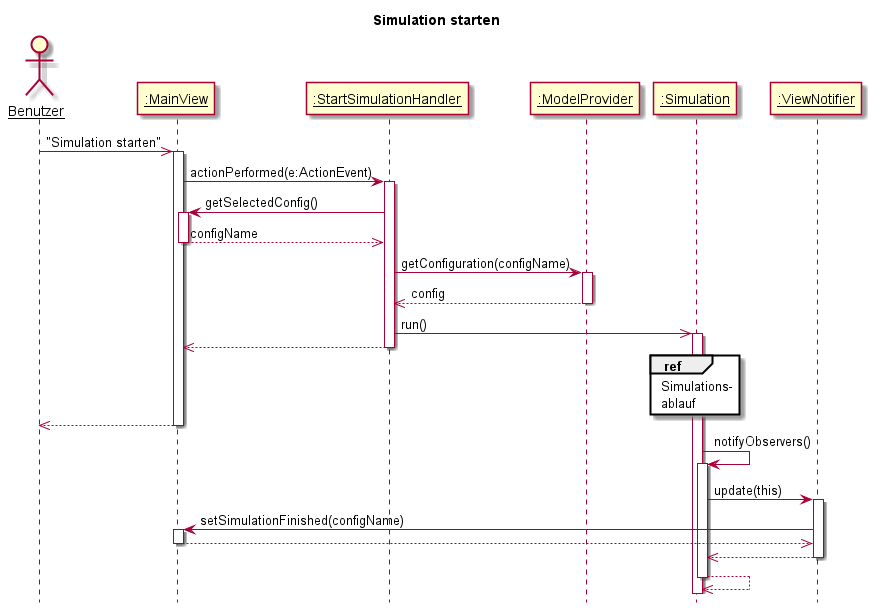
\includegraphics[width=1.0\textwidth]{sequenz_simulationstarten_mitobs}}
\bigskip


Ausgangspunkt der Sequenz "Simulation starten" ist das Drücken des entsprechenden Buttons im Hauptfenster. Zuvor hat der Benutzer die gewünschte Konfiguration oder Mehrfachkonfiguration ausgewählt.
Im Anschluss unternimmt der StartSimulationHandler die für den Start der Simulation nötigen Vorbereitungen und führt sie schließlich mit run() aus.
Hier setzt die Sequenz "Simulationsablauf" an (s.u.).
Während dem Ablauf der Simulation wird ihr Status durch den ViewNotifier überwacht. Stellt dieser fest, dass die Simulation abgeschlossen ist, benachrichtigt er das Hauptfenster, was die Sequenz beschließt.
\end{figure}

\begin{figure}[htbp]
{\centering 
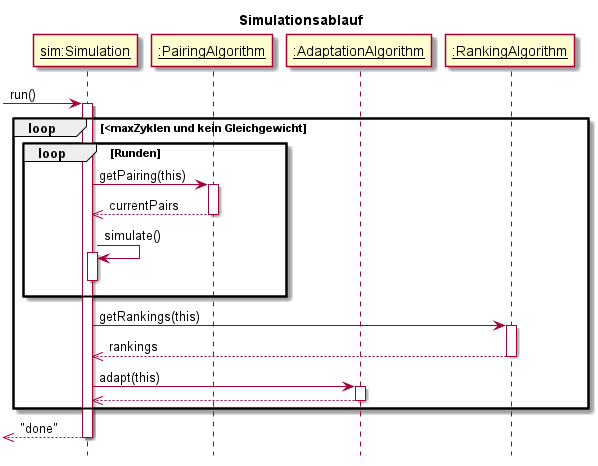
\includegraphics[width=1.0\textwidth]{sequenz_simulation}}
\bigskip


Die Sequenz "Simulationsablauf" zeigt den eigentlichen Ablauf der Simulation. Dieser besteht im Wesentlichen aus zwei verschachtelten Schleifen. Zum Ende eines jeden Zyklus wird die Simulation auf ein Gleichgewicht überprüft, was ein Abbruchkriterium der äußeren Schleife darstellt.
Die Spiele werden durch simulate() auf der Simulation selbst ausgeführt, wohingegen Manipulationen, die den Datensatz der Simulation betreffen, durch den entsprechenden Algorithmus vorgenommen werden.

\end{figure}





\newpage
\section{Ausgewählte Algorithmen}

\subsection{Bewertungsalgorithmen}

Im Folgenden werden die Bewertungsalgorithmen /F0810/ (\emph{AverageRank}) und /W0410/ (\emph{CustomCycleScore}) aus dem Pflichtenheft in Pseudocode näher beschrieben. 

\begin{lstlisting}
AverageRank:

public HashMap<Agent, Integer> getRankings(Simulation sim) 
	
	currentCycle <- sim.getCurrentCycle()
	agents <- sim.getAgents()
	ranks <- List of HashMap<Agent, Integer>	
	cycles <- max(1, currentCycle - WINDOW_SIZE)
	
	for i <- 0; i < cycles; i++ 
		ranks[i] <- rankOfAgents(agents, i, i + WINDOW_SIZE)
	
	result <- HashMap<Agent, Integer>	
	
	for Agent a in agents
		averageRank <- 0
		for i <- 0; i < cycles; i++
			averageRank <- averageRank + ranks[i].get(a)
		averageRank <- roundDown(averageRank / cycles)
		
		result.put(a, averageRank)
	
	result <- resolveConflicts(result)
	return result
\end{lstlisting}
\emph{WINDOW\_SIZE} ist die Größe des Sliding-Windows. In Zeile 8 wird sicher gestellt, dass die Schleife mindestens einmal durchlaufen wird, auch wenn \emph{WINDOW\_SIZE} größer als die bisherige Zyklenanzahl ist.
Die Hilfsmethode \emph{rankOfAgents(agents, start, end)} berechnet die Gesamtpunktzahl der Agenten von Zyklus \emph{start} bis Zyklus \emph{end} und platziert die Agenten gemäß dieser Gesamtpunktzahl in einer Rangliste. Sollte $i + WINDOW\_SIZE > currentCycle$ gelten, wird nur bis \emph{currentCycle} summiert. 
In der Schleife ab Zeile 15 wird der Durchschnittsrang von allen Agenten gebildet.
Es kann vorkommen, dass durch die Durchschnittsbildung und abrunden in Zeile 18 mehrere Agenten den gleichen Rang bekommen. Diese Konflikte werden durch \emph{resloveConflict(ranks)} gelöst. Dabei werden zuerst die Agenten nach ihrem Rang sortiert. Bei gleichem Rang hat der Agent mit der höheren Gesamtpunktzahl über alle Zyklen den höheren Rang, bei gleicher Gesamtpunktzahl ist die Platzierung zufällig. Der finale Rang der Agenten entspricht der Platzierung nach dieser Sortierung.

\begin{lstlisting}
CustomCycleScore:

public HashMap<Agent, Integer> getRankings(Simulation sim) 
	
	agents <- sim.getAgents()
	currentCycle <- sim.getCurrentCycle()
	ranks <- rankOfAgents(agents, currentCycle - WINDOW_SIZE, currentCycle)
	
	return ranks
	
\end{lstlisting}
\emph{WINDOW\_SIZE} ist die Größe des Sliding-Windows. Die Hilfsmethode \emph{rankOfAgents(agents, start, end)} ist hierbei die gleiche wie in \emph{AverageRank}. Sollte $currentCycle - WINDOW\_SIZE < 0$ gelten, wird ab dem ersten Zyklus summiert. Somit werden nur die letzten \emph{WINDOW\_SIZE} Zyklen für die Platzierung berücksichtigt. 


\subsection{Paarungsalgorithmen}

Wie bereits im Pflichtenheft spezifiziert, soll ein Paarungsalgorithmus angeboten werden, der ein Maximum an Kooperationsbereitschaft mit Hinblick auf die gesamte Population erzielt. Diese Aufgabe lässt sich auf ein klassisches Problem der Graphentheorie übertragen, und zwar das des "Maximum Weighted Perfect Matching in Simple Graphs". Dabei stellen die Agenten die Knoten des Graphen dar und die Kantengewichte die Kooperationswahrscheinlichkeiten.\\
Für das beschriebene Problem existieren zahlreiche theoretische Lösungen, etwa der \emph{Blossom algorithm} von Jack Edmonds und seine Iterationen.\\
JGraphT\footnote{\href{https://jgrapht.org/}{https://jgrapht.org/}} ist eine freie Java-Bibliothek, die u.a. Algorithmen für das Matching in Graphen zur Verfügung stellt, so etwa auch den genannten \emph{Blossom algorithm}.\\
Swiss verwendet JGraphT um die anfangs erwähnte Funktionalität zu erzielen. Zudem werden weitere – voraussichtlich schnellere – Paarungsalgorithmen angeboten, die Näherungslösungen beschreiben. Diese dienen gleichzeitig als Rücksicherung, falls nicht absehbare Komplikationen mit JGraphT auftreten sollten.


Als eine weitere Möglichkeit für den Paarungsalgorithmus verwenden wir eine Anpassung des \emph{Brute Forece Pair Matching} Algorithmus aus dem JASSS Journal\footnote{\href{http://jasss.soc.surrey.ac.uk/20/4/8.html}{Efficient and Effective Pair-Matching Algorithms for Agent-Based Models}}.

\begin{lstlisting}
Brut force pair matching:

public Pair[] getPairing(Agent[] agents) 

	shuffle(agents)
	pairs <- Pair[]
	for each unmatched agent a in agents
		best <- infinity
		for each unmatched agent b after a in agents
			d <- distance(a, b)
			if d < best
				best <- d
				bestPartner <- b
				
		pairs.addPair(a, bestPartner)
		mark a and bestPartner as paired		
	return pairs	
	
\end{lstlisting}
Für die Distanzfunktion gilt: $distance(a, b) = max(P('a kooperiert mit b'), P('b kooperiert mit a'))$. $P$ ist hierbei eine Wahrscheinlichkeitsfunktion. Wenn die kombinierte Strategien deterministisch sind gilt $distance(a, b) = 0$ genau dann, wenn $a$ und $b$ miteinander kooperieren und $distance(a, b) = 1$ genau dann, wenn $a$ mit $b$ oder $b$ mit $a$ nicht kooperiert. Sind sie nicht deterministisch können Werte zwischen 0 und 1 vorkommen.

\begin{lstlisting}
Brut force pair matching heuristic:

public Pair[] getPairing(Agent[] agents) 
	shuffle(agents)
	pairs <- Pair[]
	for each unmatched agent a in agents
		best <- infinity
		for each unmatched agent b after a in agents
			d <- distance(a, b)			
			if d < best
				best <- d
				bestPartner <- b
			if best <= epsilon
				break			
						
		pairs.addPair(a, bestPartner)
		mark a and bestPartner as paired
	return pairs		
	
\end{lstlisting}
Eine weitere mögliche Anpassung ist zwei Agenten zu Paaren, wenn $distance(a, b) \leq \epsilon$ gilt für $\epsilon \geq 0$. Dadurch werden Agenten gepaart, die sehr wahrscheinlich miteinander kooperieren. Man beachte, dass für $\epsilon = 0$ der Algorithmus identisch zu dem Ersten ist. Allerdings hat er in vielen Fällen eine schneller Laufzeit, da sobald ein Agent gefunden wurde, sodass beide kooperieren, dieser mit ihm gepaart wird.

\end{document}